\documentclass{article}
\usepackage[a4paper, total={6in, 8in}]{geometry}
\usepackage[italian]{babel}
\usepackage[T1]{fontenc}
\usepackage{graphicx} 
\usepackage{amsmath}
\usepackage{amssymb}
\usepackage{mathtools}
\usepackage{enumitem}
\usepackage{wrapfig}
\usepackage{hyperref}
\hypersetup{
    colorlinks=true,
    linkcolor=blue,
    filecolor=magenta,      
    urlcolor=blue,
}

\begin{document}
\part{Insiemi numerici}
\section{Numeri naturali}
$\mathbb{N} = \{0, 1, 2, ...\}$ \\

\noindent\textbf{NB!} L'insieme $\mathbb{N}$ comprende anche lo 0. \\

\noindent Le operazioni possibili sono l'addizione e la moltiplicazione.

\subsection{Addizione}
\begin{equation*}
    +: \mathbb{N} \times \mathbb{N} \xrightarrow{} \mathbb{N} \qquad \qquad (a,b) \longmapsto a + b
\end{equation*}

\subsubsection{Assiomi}
\noindent\textbf{NB!} Un assioma è una proprietà che vale senza dover essere dimostrata. In altre parole, è presa per vera. \\

\noindent Dati $a, b, c \in \mathbb{N}$, si hanno le seguenti proprietà: 

\begin{itemize}
    \item \textbf{Commutativa}: $a + b = b + a$
    \item \textbf{Associativa}: $(a + b) + c = a + (b + c)$
\end{itemize}

\noindent\textbf{NB!} Si può dimostrare che esiste ed è unico l'elemento neutro $e_0$, cioè quell'elemento che aggiunto ad $a$ non fa cambiare il risultato della somma. Tale elemento è proprio lo 0, infatti:

\begin{equation*}
    a + e_0 = a + 0 = a \qquad \forall a \in \mathbb{N}
\end{equation*}

\subsection{Moltiplicazione}
\begin{equation*}
    \cdot: \mathbb{N} \times \mathbb{N} \xrightarrow{} \mathbb{N} \qquad \qquad (a,b) \longmapsto a \cdot b
\end{equation*}

\subsubsection{Assiomi}
Dati $a, b, c \in \mathbb{N}$, si hanno le seguenti proprietà: 

\begin{itemize}
    \item \textbf{Commutativa}: $a \cdot b = b \cdot a$
    \item \textbf{Associativa}: $(a \cdot b) \cdot c = a \cdot (b \cdot c)$
\end{itemize}

\noindent\textbf{NB!} Si può dimostrare che esiste ed è unico l'elemento neutro $e_1$, cioè quell'elemento che moltiplicato ad $a$ non fa cambiare il risultato. In particolare, si ha che $e_1 = 1$, infatti:

\begin{equation*}
    a \cdot e_1 = a \cdot 1 = a \qquad \forall a \in \mathbb{N}
\end{equation*}

\subsection{Ordinamento totale}
L'insieme $\mathbb{N}$ è totalmente ordinato, ovvero dati due numeri riesco a capire qual è il maggiore e quale il minore. In linguaggio matematico possiamo scrivere: 

\begin{equation*}
    a \leq b \underset{def}{\Longleftrightarrow} \exists \ c \in \mathbb{N} \ | \ a + c = b
\end{equation*}

\noindent\textbf{NB!} Non tutti gli insiemi sono totalmenti ordinati. Ad esempio, i numeri complessi non lo sono.

\subsubsection{Proprietà dell'ordinamento}
\begin{itemize}
    \item \textbf{Riflessiva}: $a \leq a \qquad \forall a \in \mathbb{N}$
    \item \textbf{Antisimmetrica}: è un modo di mostrare che due numeri sono uguali. $$\forall a,b \in \mathbb{N} \quad se \quad \begin{cases}
        a \leq b \\ 
        b \leq a
    \end{cases} \quad allora \quad a = b$$ \noindent Questa è anche la struttura tipica di un \textbf{enunciato}.
    
    \item \textbf{Transitiva}: $\forall a, b, c \in \mathbb{N} \quad se \quad a \leq b \ e \ b \leq c \quad allora \quad a \leq c$.
    \item \textbf{Dicotomia}: $\forall a,b \in \mathbb{N}$, si ha che: $a \leq b \ oppure \ b \leq a$ (essendoci "oppure", significa che o sono entrambe vere o una è vera e l'altra è falsa).
\end{itemize}

\noindent Se ho $\forall a,b,c \in \mathbb{N} \quad a \leq b$, cosa succede se aggiungo $c$? $a +c \leq b + c$. Il segno non cambia grazie alla \textbf{compatibilità dell'ordinamento rispetto alla somma}. \\
Lo stesso vale per la \textbf{compatibilità dell'ordinamento rispetto al prodotto} quando si hanno $\forall a,b,c \in \mathbb{N}, \quad se \quad a \leq b \ e \ c > 0 \implies ac \leq bc$.

\subsection{Struttura di un teorema}
Un teorema possiede sempre: 

\begin{itemize}
    \item un \textbf{enunciato}, avente la seguente struttura: \textit{Se \textbf{ipotesi}, allora \textbf{tesi}};
    \item una \textbf{dimostrazione} dell'enunciato, ovvero un procedimento di deduzione che parte dalla verità delle ipotesi per dimostrare la verità delle tesi.
\end{itemize}

\noindent La dimostrazione può utilizzare l'\textbf{implicazione diretta} del tipo $A \implies B$ oppure l'\textbf{implicazione contronominale} del tipo $\lnot b \implies \lnot a$ (utilizzato nelle dimostrazioni per assurdo/contraddizione). \\
In molti casi, inoltre, si costruisce una contraddizione con un'altra proprietà $c$ (con $c \neq a$):

\begin{equation*}
    \lnot b \implies \begin{cases}
        c \ è \ vero \\
        \lnot c \ è \ vero
    \end{cases}
\end{equation*}

\subsection{Principio di induzione}
\noindent\textbf{NB!} Si chiama "principio", ma è un teorema. \\

\noindent Sia $A \subseteq \mathbb{N}$ e $p \in \mathbb{N}$. Assumiamo che siano valide le seguenti ipotesi: 

\begin{enumerate}
    \item $p \in A$ (questa ipotesi è chiamata \textbf{passo base});
    \item $se \ n \in A \implies n + 1 \in A$ (questa ipotesi è chiamata \textbf{passo induttivo}).
\end{enumerate}

\noindent Allora $\{n \in \mathbb{N} \ | \ n \geq p \} \subseteq A$.

\subsubsection{Esempio 1 di utilizzo del principio di induzione}
Dimostriamo che $\forall n \in \mathbb{N}, \ con \ n \geq 1$, vale: 

\begin{equation}
    \sum_{i = 1}^n i = \frac{n (n + 1)}{2}
\label{eq:1}
\end{equation}

\noindent Lo scopo, quindi, è dimostrare che $A = \{ n \in \mathbb{N} \ |$ (\ref{eq:1}) è vera \}.\\

\noindent Innanzitutto, fissiamo il punto base $p = 1$, essendo che la formula deve essere dimostrata per tutti i numeri naturali $n$, che siano maggiori o uguali a 1. Ma $p = 1 \in A$? Verifichiamolo:

\begin{equation*}
    \sum_{i = 1}^1 i = 1 \qquad \frac{1 \cdot (1 + 1)}{2} = 1
\end{equation*}

\noindent Ciò significa che per $p = 1$, (\ref{eq:1}) è vera, ovvero che il passo base è stato verificato. Ma la formula è vera per tutti $n \in \mathbb{N}$? Non lo so, finché non verifico il passo induttivo, cioè $se \ n \in A \implies n+1 \in A$. Scomponiamo il passo induttivo in ipotesi e tesi ed otteniamo: 

\begin{itemize}
    \item Ipotesi induttiva: $$\sum_{i = 1}^n i = \dfrac{n(n+1)}{2}$$
    \item Tesi induttiva: $$\sum_{i = 1}^{n+1} i = \dfrac{(n+1)(n+2)}{2}$$
\end{itemize}

\noindent Noi ovviamente dobbiamo verificare la tesi. Partiamo quindi da quest'ultima. Attraverso la proprietà associativa della somma possiamo riscriverla come segue:

\begin{equation*}
    \sum_{i = 1}^{n+1} i = \sum_{i = 1}^n i + (n + 1)
\end{equation*}

\noindent Siamo così riusciti a ricondurre il calcolo ad un oggetto noto (l'ipotesi induttiva). Possiamo quindi riscrivere: 

\begin{equation*}
    \sum_{i = 1}^{n+1} i = \frac{n(n+1)}{2} + (n+1)
\end{equation*}

\noindent A questo punto, svolgiamo il denominatore comune e raccogliamo $(n+1)$:

\begin{equation*}
    \sum_{i = 1}^{n+1} i = \frac{(n+1)(n+2)}{2}
\end{equation*}

\noindent Siamo così riusciti a verificare il passo induttivo. Una volta verificato passo base e passo induttivo, possiamo finalmente usare il \textbf{principio di induzione} e quindi dire che $A = \{ n \in \mathbb{N} \ | \ n \geq 1 \}$.

\subsubsection{Esempio 2 di utilizzo del principio di induzione}
Sia $q \in \mathbb{R} - \{ 0, 1 \}$, dimostriamo che: 

\begin{equation}
    \sum_{k = 0}^n q^k = \frac{1-q^{n+1}}{1-q} \quad \forall n \in \mathbb{N}
    \label{eq:2}
\end{equation}

\noindent Poniamo $p = 0$ come passo base (è infatti il valore minimo tra i numeri naturali a cui appartiene $n$) e verifichiamo che esso verifichi la formula: 

\begin{equation*}
    \sum_{k = 0}^n q^k = q^0 = 1 \qquad \frac{1 - q}{1 - q} = 1
\end{equation*}

\noindent Ciò significa che per $p = 0$, (\ref{eq:2}) è vera, ovvero che il passo base è stato verificato. Ma la formula è vera per tutti $n \in \mathbb{N}$? Non lo so, finché non verifico il passo induttivo, cioè $se \ n \in A \implies n+1 \in A$. Scomponiamo il passo induttivo in ipotesi e tesi ed otteniamo: 

\begin{itemize}
    \item Ipotesi induttiva: $$\sum_{k = 0}^n q^k = \frac{1-q^{n+1}}{1-q}$$
    \item Tesi induttiva: $$\sum_{k = 0}^{n + 1} q^k = \frac{1-q^{n+2}}{1-q}$$
\end{itemize}

\noindent Noi ovviamente dobbiamo verificare la tesi. Partiamo quindi da quest'ultima. Attraverso la proprietà associativa della somma possiamo riscriverla come segue:

\begin{equation*}
    \sum_{k = 0}^{n + 1} q^k = \sum_{k = 0}^n q^k + q^{n + 1}
\end{equation*}

\noindent Siamo così riusciti a ricondurre il calcolo ad un oggetto noto (l'ipotesi induttiva). Possiamo quindi riscrivere: 

\begin{equation*}
    \sum_{k = 0}^{n + 1} q^k = \frac{1-q^{n+1}}{1-q} + q^{n + 1}
\end{equation*}

\noindent Svolgiamo ora i calcoli:

\begin{equation*}
    \sum_{k = 0}^{n + 1} q^k = \frac{1-q^{n+1} + q^{n+1} - q\cdot q^{n+1}}{1-q} = \frac{1-q^{n+1} + q^{n+1} - q^{n+2}}{1-q} = \frac{1 - q^{n+2}}{1-q}
\end{equation*}

\noindent Siamo così riusciti a verificare il passo induttivo. Una volta verificato passo base e passo induttivo, possiamo finalmente usare il \textbf{principio di induzione} e quindi dire che $A = \{ n \in \mathbb{N} \ | \ n \geq 0 \}$. Essendo poi che $\mathbb{N}$ contiene già tutti i numeri maggiori o uguali a zero, possiamo direttamente dire che la proprietà è verificata $\forall n \in \mathbb{N}$. \\

\noindent\textbf{NB!} Possiamo estendere la proprietà anche nel caso in cui $q = 0$. Per convenzione, infatti, con i numeri naturali si ha che $0^0 = 1$. Per cui verifichiamo che l'uguaglianza sia ancora mantenuta:

\begin{equation*}
    \sum_{k=0}^n q^k = 0^0 + 0^1 + 0^2 + ... = 1 + 0 + 0 + ... = 1 \qquad \frac{1 - 0^1}{1 - 0} = 1
\end{equation*}

\section{Numeri interi}
$\mathbb{Z} = \mathbb{N} \cup (- \mathbb{N})$ \\

\noindent\textbf{NB!} Per definizione si ha che un "-" insieme equivale a:

\begin{equation*}
    -A \vcentcolon = \{ -a \ | \ a \in A \}
\end{equation*}

\subsection{Assioma di esistenza dell'opposto}
$\forall m \in \mathbb{Z} \ \exists n \in \mathbb{Z} \ | \ m + n = 0$

\subsection{Compatibilità dell'ordinamento}
Se $a,b,c \in \mathbb{Z}$, abbiamo due casi: 

\begin{itemize}
    \item $a \leq b, c > 0 \implies ac \leq bc$
    \item $a \leq b, c < 0 \implies ac \geq bc$
\end{itemize}

\noindent\textbf{Problema!} $a \in \mathbb{Z}, \ \exists b \in \mathbb{Z} \ | \ ab = 1$? Sì, ma ce ne sono solo due: $a \in \{ -1, 1 \}$. In particolare, $b$ è l'inverso del punto $a$. In simboli: $b \vcentcolon = a^{-1}$.

\section{Numeri razionali}
$\mathbb{N} \subsetneq \mathbb{Z} \subsetneq \mathbb{Q}$. In particolare:

\begin{equation*}
    \mathbb{Q} = \{ m \cdot n^{-1} \ | \ m \in \mathbb{Z}, n \in \mathbb{N} - \{ 0 \}, mcd(m,n) = 1 \}
\end{equation*}

\noindent Si nota quindi che $m$ e $n$ sono \textbf{coprimi} perché non hanno divisori comuni (per questo hanno $mcd(m,n) = 1$). \\

\noindent\textbf{NB!} In $\mathbb{Q}$ vale l'\textbf{assioma dell'inverso moltiplicativo} (ovviamente solo per i numeri che me lo permettono. Ad esempio, con 0 non vale), cioè: 

\begin{equation*}
    \forall a \in \mathbb{Q} - \{ 0 \}, \ \exists b \in \mathbb{Q} \ | \ ab = 1 \qquad (dove \ b = a^{-1})
\end{equation*}

\subsection{Dimostrazione di un polinomio senza soluzioni razionali}
\noindent Notiamo ora però che i numeri razionali non ci bastano ancora. Infatti, se prendiamo un polinomio come $p(x) = x^2 - 2$, in cui si ha che $p \in \mathbb{Q}[x]$ (ovvero un polinomio a coefficienti in $\mathbb{Q}$), non si hanno soluzioni razionali per $x^2 - 2 = 0$. Dimostriamo ora per contraddizione questo teorema: \\

\noindent Supponiamo che $\exists \dfrac{m}{n} \in \mathbb{Q} \ | \ \left(\dfrac{m}{n}\right)^2 = 2; \ mcd(m,n) = 1$ (stiamo quindi negando la tesi). Svolgiamo ora dei semplici calcoli:

\begin{equation*}
    \left(\dfrac{m}{n}\right)^2 = 2
\end{equation*}

\begin{equation*}
    \dfrac{m^2}{n^2} = 2
\end{equation*}

\begin{equation*}
    m^2= 2n^2
\end{equation*}

\noindent Essendoci il fattore $2$, $2n^2$ è sicuramente un \textbf{numero pari}, perché può essere diviso per $2$.

\subsubsection{Lemma: un numero elevato al quadrato che è pari è un numero pari}
Immaginiamo di avere un $m$ dispari, che può anche essere scritto come: $m = 2k + 1 \quad con \ k \in \mathbb{Z}$ (ovvero come un numero pari $2k$, trasformato in dispari dall'aggiunta di $1$).\\
Ipotizziamo ora di dover calcolare $m^2$ come nella dimostrazione qui sopra:

\begin{equation*}
    m^2 = (2k + 1)^2 = 4k^2 + 4k + 1 = 4k(k + 1) + 1
\end{equation*}

\noindent Notiamo quindi ancora una volta come, elevando al quadrato un numero dispari $m$, otteniamo nuovamente un numero dispari (perché $4k(k+1)$ è pari, ma è trasformato in dispari dall'aggiunta di $1$).\\

\noindent Ritorniamo ora alla dimostrazione: sapendo che $m^2$ è pari, allora $m$ sarà per forza pari per il lemma qui sopra. Essendo pari, si ha che: $\exists h \in \mathbb{Z} \ | \ m = 2h$ (ovvero stiamo dicendo che $m$ è divisibile per $2$). \\
Riprendiamo ora l'ipotesi di partenza e svolgiamo alcuni calcoli:

\begin{equation*}
    m^2 = 2n^2
\end{equation*}

\begin{equation*}
    (2h)^2 = 2n^2
\end{equation*}

\begin{equation*}
    4h^2 = 2n^2
\end{equation*}

\begin{equation*}
    2h^2 = n^2
\end{equation*}

\noindent Essendo $2h^2$ un numero pari, allora anche $n^2$ è un numero pari e, per lo stesso ragionamento fatto sul lemma, anche $n$ è pari. Arriviamo quindi ad una contraddizione: sia $m$, che $n$ sono numeri pari, ciò significa che $mcd(m,n) \neq 1$ (ovvero non sono numeri coprimi, ma sono in realtà divisibili tra loro). Possiamo così confermare il fatto che non esistono soluzioni razionali a $p(x)$, infatti $\sqrt{2} \notin \mathbb{Z}$. Più in generale, si può dire che $x^2 - p = 0$, dove $p$ è un numero primo, non ha soluzioni razionali ($\sqrt{p} \notin \mathbb{Q})$.\\

\noindent\textbf{NB!} I numeri primi sono i numeri diversi da 1, con fattori solo 1 e se stessi.

\subsection{Fattoriale}
Diamo una definizione induttiva del fattoriale di $n \in \mathbb{N}: n!$: 

\begin{itemize}
    \item $0! = 1$
    \item $(n+1)! \vcentcolon = (n+1)(n!) \qquad \forall n \geq 1$
\end{itemize}

\noindent Per il principio di induzione, $n!$ è ben definito $\forall n \in \mathbb{N}$. \\

\noindent Possiamo anche definirlo come:

\begin{equation*}
    n! = \prod_{i=1}^n i = \vcentcolon 1 \cdot 2 \cdot 3 \cdot 4 \cdot ... \cdot n
\end{equation*}

\subsubsection{Dimostrazione}
Dimostriamo la seguente proposizione: $n! \geq n \quad \forall n \in \mathbb{N}$. Prendiamo innanzitutto un passo base e un passo induttivo:

\begin{itemize}
    \item $p = 0: \quad 0! = 1 \implies 1 \geq 0$. Ciò significa che il passo base è verificato
    \item se $n! \geq n$, allora $(n+1)! \geq (n+1)$
\end{itemize}

\noindent Riscriviamo quindi la tesi, cercando un oggetto noto (l'ipotesi):

\begin{equation*}
    (n+1)! = (n+1)(n!)
\end{equation*}

\noindent Abbiamo già precedentemente dimostrato come $n! \leq n$. Moltiplichiamo ora a destra e a sinistra questa disequazione per $(n+1)$: il verso della disequazione non cambia, essendo che tale numero è sicuramente positivo. Otteniamo quindi:

\begin{equation*}
    (n+1)! = (n+1)(n!) \geq (n+1)n
\end{equation*}

\noindent Avendo quindi mostrato come $(n+1)! \geq (n+1)n$, se riusciamo a dimostrare che $(n+1)n \geq (n+1)$ il gioco è fatto! Essendo che $n \geq 1$, significa che $(n+1) \geq 2$. Capiamo quindi che $(n+1)n \geq (n+1)$ e quindi scritto tutto in una riga:

\begin{equation*}
    (n+1)! \geq (n+1)n \geq (n+1)
\end{equation*}

\subsection{Coefficiente binomiale}
Dati $n, k \in \mathbb{N}$, abbiamo che:

\begin{itemize}
    \item se $k \leq n$: $$\binom{n}{k} \vcentcolon = \dfrac{n!}{k!(n-k)!}$$
    \item se $k > n$: $$\binom{n}{k} \vcentcolon = 0$$
\end{itemize}

\subsubsection{Proprietà del coefficiente binomiale}
\begin{equation*}
    \binom{n}{0} = \frac{n!}{0!(n - 0)!} = \frac{n!}{n!} = 1
\end{equation*}

\begin{equation*}
    \binom{n}{n} = \frac{n!}{n!(n - n)!} = \frac{n!}{n!} = 1
\end{equation*}

\begin{equation*}
    \binom{n}{n-1} = \frac{n!}{(n-1)!(n-(n-1))!} = \frac{n!}{(n-1)!} = \frac{n(n-1)!}{(n-1)!} = n
\end{equation*}

\begin{equation*}
    \binom{n}{k} = \frac{n!}{k!(n-k)!} = \frac{n!}{(n-k)!(n-(n-k))!} = \binom{n}{n-k} \qquad \forall k \leq n
\end{equation*}

\begin{equation*}
    \binom{n}{k} \in \mathbb{N} \quad \forall k,n \in \mathbb{N}
\end{equation*}

\subsubsection{Dimostrazione di una delle proprietà del coefficiente binomiale}
\begin{equation*}
    \binom{n}{k} = \binom{n-1}{k-1} + \binom{n-1}{k}
\end{equation*}

\begin{equation*}
    \binom{n}{k} = \binom{n-1}{k-1} + \binom{n-1}{k} = \frac{(n-1)!}{(k-1)!(n-k)!} + \frac{(n-1)!}{k!(n-1-k)!} \quad con \ 1 \leq k \leq n
\end{equation*}

\begin{equation*}
    \binom{n}{k} = \frac{(n-1)!}{(k-1)!(n-k)(n-k-1)!} + \frac{(n-1)!}{k(k-1)!(n-1-k)!}
\end{equation*}

\begin{equation*}
    \binom{n}{k} = \frac{(n-1)!}{(k-1)!(n-k-1)!} \cdot \left(\frac{1}{n-k} + \frac{1}{k}\right)
\end{equation*}

\begin{equation*}
    \binom{n}{k} = \frac{(n-1)!}{(k-1)!(n-k-1)!} \cdot \left(\frac{n}{k(n-k)}\right)
\end{equation*}

\begin{equation*}
    \binom{n}{k} = \frac{n!}{k!(n-k)!}
\end{equation*}

\section{Numeri reali}
$\mathbb{N} \subsetneq \mathbb{Z} \subsetneq \mathbb{Q} \subsetneq \mathbb{R}$ \\

\noindent\textbf{NB!} Sull'insieme $\mathbb{R}$ valgono tutti gli assiomi definiti precedentemente!

\subsection{Assioma di separazione}
Prendiamo due insiemi $A$ e $B$ con $A \neq \varnothing \neq B$ tali che $a \leq b \quad \forall a \in A, \forall b \in B$ (dato che tutti gli elementi di $A$ sono più piccoli di quelli di $B$, i due insiemi si dicono \textbf{separati}), allora: 

\begin{equation*}
    \exists x \in \mathbb{R} \ | \ a \leq x \leq b \quad \forall a \in A, \forall b \in B
\end{equation*}

\noindent dove $x$ è detto \textbf{separatore} di $A$ e $B$.

\subsection{Proprietà di Archimede con relativa dimostrazione}
\begin{equation*}
    \forall x \in \mathbb{R}, \exists n \in \mathbb{N} \ | \ n > x
\end{equation*}

\noindent Dimostriamo per contraddizione questa proprietà. Innanzitutto verifichiamo il caso in cui $x \leq 0$. Dal momento che $\mathbb{N}$ contiene numeri maggiori o uguali a 0, la proprietà è già verificata. \\
Studiamo ora il caso in cui $x > 0$: definiamo l'insieme $A$ come segue: $A \vcentcolon = \{ n \in \mathbb{N} \ | \ n \leq x \} \subseteq \mathbb{N}$. La nostra tesi è che $A \neq \mathbb{N}$, cioè che $\exists m \notin A$ (perché $m > x$). Supponiamo allora che $A = \mathbb{N} \neq \varnothing$. Sia ora $B \vcentcolon = \{ y \in \mathbb{R} \ | \ y \geq n, \forall n \in \mathbb{N} \}$. Se $A = \mathbb{N}$, allora tutti i numeri naturali sono più piccoli di $x$. Per questo motivo possiamo dire che $x$ "fa il gioco" di $y$ (ovvero è un numero reale, maggiore di tutti i numeri naturali). Quindi $x \in B$, per cui ne deriva che $B \neq \varnothing$. \\
Dato che $\forall y \in B$ si ha che $y \geq n \quad \forall n \in A \ (= \mathbb{N})$, allora significa che $A$ e $B$ sono insiemi separati. Per questo motivo, possiamo sfruttare l'assioma di separazione: $\exists \lambda \in \mathbb{R} \ | \ n \leq \lambda \leq y \quad \forall n \in A \ (= \mathbb{N}), \forall y \in B$. Dato che $n+1 \in \mathbb{N}$, è vero che $n+1 \leq \lambda \leq y$. \\
Concentriamoci ora sulla prima parte della disequazione $n+1 \leq \lambda$ e riscriviamola come $n \leq \lambda - 1 \quad \forall n \in A \ (= \mathbb{N})$. Dato che $\lambda$ è un numero reale maggiore o uguale di ogni numero naturale, anche $\lambda - 1$ lo è. Per cui possiamo dire che $\lambda - 1 \in B$. Infine, per definizione $\lambda$ è elemento separatore di $A$ e $B$, quindi: $(n \leq) \ \lambda \leq y \quad \forall y \in B, \forall n \in A$. Quindi, possiamo sostituire il generico elemento $y$ di $B$, con $\lambda - 1$ e otteniamo $\lambda \leq \lambda - 1 \implies 1 \leq 0$, che è una contraddizione.

\subsection{Proprietà della parte intera}
$\forall x \in \mathbb{R}, \ \exists ! \ n \in \mathbb{Z} \ | \ n \leq x < n + 1$ \\

\noindent\textbf{NB!} $n$ è detto \textbf{parte intera} di $x$ e si indica con $n = \lfloor x \rfloor$.

\subsubsection{Grafici della parte intera}
\begin{figure}[!h]
    \centering
    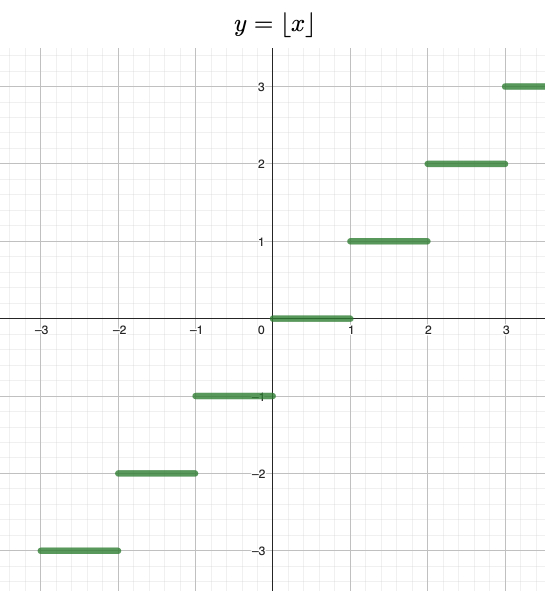
\includegraphics[width=7cm]{./images/floor_graph.jpg}\hfill
    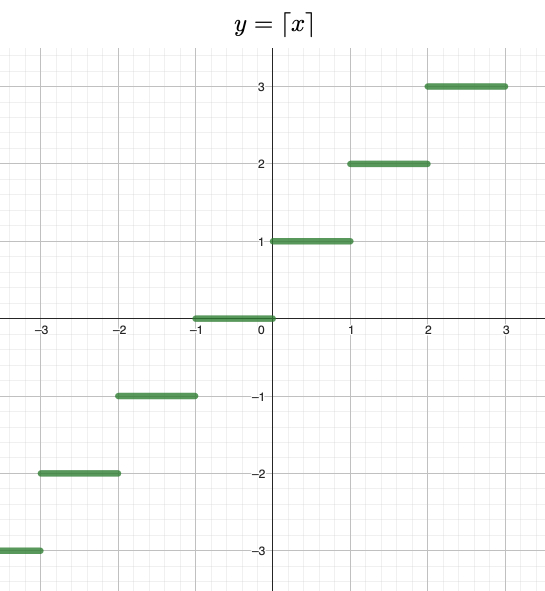
\includegraphics[width=7cm]{./images/ceil_graph.jpg}
\end{figure}

\noindent \textbf{NB!} Non è vero che $\lceil x \rceil = \lfloor x \rfloor + 1 \quad \forall x \in \mathbb{R}$, ma è vero solo per $x \in \mathbb{R} - \mathbb{Z}$.

\subsection{Teorema della densità dei razionali nei reali e relativa dimostrazione}
\begin{center}
    $\forall x \in \mathbb{R}, \forall \varepsilon > 0, \exists z \in \mathbb{Q} \ | \ z \leq x < z + \varepsilon \quad dove \ \varepsilon \in \mathbb{R}$
    \begin{figure}[!h]
    \centering
    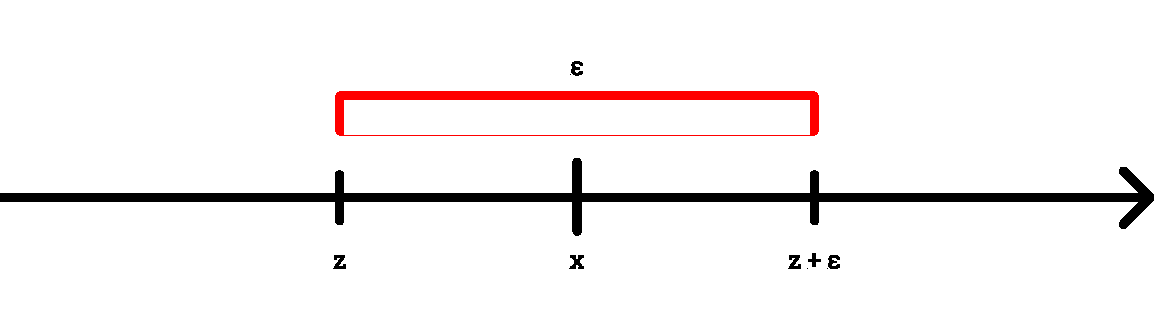
\includegraphics[width=15cm]{./images/densityQinR.pdf}
\end{figure}
\end{center}

\noindent Dimostriamo ora questo teorema. Sia $x \in \mathbb{R}, \varepsilon > 0$. Allora $\dfrac{1}{\varepsilon} > 0$. Utilizziamo ora la proprietà di Archimede:

\begin{equation*}
    \exists q \in \mathbb{N} \ | \ q > \frac{1}{\varepsilon} > 0
\end{equation*}

\noindent Consideriamo ora $qx \in \mathbb{R}$ e usiamo la proprietà della parte intera: 

\begin{equation*}
    \exists p \in \mathbb{N} \ | \ p \leq qx < p + 1
\end{equation*}

\noindent Dividiamo ora per $q$ (essendo $q > 0$, il verso della disequazione non cambia): 

\begin{equation*}
    \frac{p}{q} \leq x < \frac{p}{q} + \frac{1}{q} \qquad dove \ \frac{p}{q} \in \mathbb{Q}
\end{equation*}

\noindent Ma essendo che $q > \dfrac{1}{\varepsilon}$ per la proprietà di Archimede, possiamo anche dire che $q\varepsilon > 1$ e che $\varepsilon > \dfrac{1}{q}$. Ne segue quindi che: 

\begin{equation*}
    \frac{p}{q} \leq x < \frac{p}{q} + \varepsilon \qquad dove \ \frac{p}{q} = z
\end{equation*}

\subsection{Teorema}
Se $a, b \in \mathbb{R}$ con $a < b$, allora: 

\begin{itemize}
    \item $\exists r \in \mathbb{Q} \ | \ a < r < b$ (ovvero tra due numeri reali, c'è sempre un razionale, purché $a \neq b$);
    \item $\exists \alpha \in \mathbb{R} - \mathbb{Q} \ | \ a < \alpha < b$ (ovvero tra due numeri reali, c'è sempre un irrazionale, purché $a \neq b$).
\end{itemize}

\subsection{Intervalli}
Esistono tre tipi di intervalli: 

\begin{itemize}
    \item \textbf{intervalli aperti}: $(a,b) = \{ x \in \mathbb{R} \ | \ a < x < b \}$;
    \item \textbf{intervalli semichiusi}: $(a,b] = \{ x \in \mathbb{R} \ | \ a < x \leq b \}$ oppure $[a,b) = \{ x \in \mathbb{R} \ | \ a \leq x < b \}$;
    \item \textbf{intervalli chiusi}: $[a,b] = \{ x \in \mathbb{R} \ | \ a \leq x \leq b \}$.
\end{itemize}

\noindent Dato $A \subseteq \mathbb R$ con $A \neq \varnothing$, $A$ si dice intervallo se e solo se $\forall x_1, x_2 \in A, \ x_1 < x_2$ si ha che $\{ x \in \mathbb{R} \ | \ x_1 < x < x_2 \} \subset A$. \\
Ad esempio, $A = (0,1) \cup \{2\}$ non è un intervallo perché se prendo $x_1 = \dfrac{1}{2}$ e $x_2 = 2$, noto come $x = \dfrac{3}{2} \notin A$. 

\subsection{Maggioranti-minoranti, insiemi superiormente-inferiormente limitati}
Dato $A \subseteq B$ con $A \neq \varnothing$, diremo che:

\begin{enumerate}
    \item $x \in \mathbb{R}$ è \textbf{maggiorante} di $A$ se e solo se $a \leq x \quad \forall a \in A$;
    \item $x \in \mathbb{R}$ è \textbf{minorante} di $A$ se e solo se $a \geq x \quad \forall a \in A$.
\end{enumerate}

\noindent Diremo quindi che $A$ è inferiormente (superiormente) limitato se e solo se esiste un minorante (maggiorante) di A. \\
Ad esempio, se $A = (0,1) \cup \{2\}$, esso è un insieme inferiormente limitato da 0 (minorante) e superiormente limitato da 2 (maggiorante). Si dice perciò che è un insieme \textbf{limitato}.

\subsubsection{Proprietà degli insiemi inferiormente/superiormente limitati}
Sia $A \subseteq \mathbb{R}$ con $A \neq \varnothing$. Se $A$ è inferiormente limitato, allora $B \subseteq A$ è anch'esso inferiormente limitato. \\

\noindent Dimostriamo questa proprietà. Dato che $A$ è inferiormente limitato, significa che esso possiede un minorante, in simboli $\exists x \in \mathbb{R} \ | \ x \leq a \quad \forall a \in A$. Ora, se un punto $b \in B$, allora $b \in A$ perché $B \subseteq A$. Proprio per questo motivo, $x \leq b \quad \forall b \in B \subseteq A$. Allora $x$ è un minorante di $B$ e quindi $B$ è inferiormente limitato. \\

\noindent Dimostriamo ora il caso di un insieme superiormente limitato. Dato quindi che $A$ è superiormente limitato, esso possiede un maggiorante, in simboli $\exists x \in \mathbb{R} \ | \ x \geq a \quad \forall a \in A$. Ora, se un punto $b \in B$, allora $b \in A$ perché $B \subseteq A$. Proprio per questo motivo, $x \geq b \quad \forall b \in B \subseteq A$. Allora $x$ è un maggiorante di $B$ e quindi $B$ è superiormente limitato.

\subsubsection{Insieme $\mathbb{N}$: inferiormente-superiormente limitato?}
Dato che i numeri naturali soddisfano la seguente condizione $n \geq 0 \quad \forall n \in \mathbb{N}$, significa che 0 è un minorante di $\mathbb{N}$ e che perciò $\mathbb{N}$ è inferiormente limitato.\\
Ma $\mathbb{N}$ è superiormente limitato? Se fosse vero, significherebbe che $\exists x \in \mathbb{R} \ | \ n \leq x \quad \forall n \in \mathbb{N}$, ma ciò va in contraddizione con la proprietà di Archimede. Perciò $\mathbb{N}$ non è superiormente limitato.

\subsubsection{Insieme $\mathbb{Z}$: inferiormente-superiormente limitato?}
Dato che $\mathbb{N}$ non è superiormente limitato e che $\mathbb{N} \subseteq \mathbb{Z}$, ne segue che neanche $\mathbb{Z}$ è superiormente limitato.\\

\noindent Ma $\mathbb{Z}$ è inferiormente limitato? Supponiamo che lo sia, ovvero che $\exists b \in \mathbb{R} \ | \ b \leq z, \forall z \in \mathbb{Z}$. Essendo che $\mathbb{Z}$ è composto anche da numeri negativi, sappiamo che $b$ deve essere sicuramente negativo ($b < 0$). Ne segue che $-b > 0$. Quindi riprendendo il ragionamento:

\begin{equation*}
    b \leq z \implies -b \geq -z \quad \forall z \in \mathbb{Z} \iff -b \geq w \quad \forall w \in \mathbb{Z}
\end{equation*}

\noindent Arriviamo così ad una contraddizione perché stiamo dicendo che $-b$, un numero positivo, è minorante di $\mathbb{Z}$, quando sappiamo benissimo che esso contiene anche numeri negativi. Per questo motivo, possiamo concludere che $\mathbb{Z}$ non è inferiormente limitato.

\subsubsection{Insieme $\mathbb{Q}$: inferiormente-superiormente limitato?}
Dato che né $\mathbb{N}$, né $\mathbb{Z}$ sono superiormente limitati, allora nemmeno $\mathbb{Q}$ è superiormente limitato. Inoltre, dato che $\mathbb{Z}$ non è inferiormente limitato, allora nemmeno $\mathbb{Q}$ è inferiormente limitato.

\subsubsection{Insieme $\mathbb{R}$: inferiormente-superiormente limitato?}
Dato che $\mathbb{N}$, $\mathbb{Z}$ e $\mathbb{Q}$ non sono superiormente limitati, allora nemmeno $\mathbb{R}$ è superiormente limitato. Inoltre, dato che né $\mathbb{Z}$, né $\mathbb{Q}$ sono inferiormente limitati, allora nemmeno $\mathbb{R}$ è inferiormente limitato.

\subsection{Massimi e minimi}
\textbf{Def:} Sia $A \subseteq R, A \neq \varnothing$, allora diremo che $A$ ammette massimo (minimo) se e solo se

\begin{equation*}
    \exists x_0 \in A \ | \ x_0 \geq a \ (x_0 \leq a) \quad \forall a \in A
\end{equation*}

\noindent In altre parole, se $x_0$ è maggiorante (minorante) di $A$ ed esso appartiene ad $A$, allora $x_0$ sarà un massimo (minimo).\\

\noindent\textbf{ES.} Prendiamo, ad esempio, $A = (0, 1]$. Sicuramente, ogni $x \geq 1$ sarà un maggiorante di $A$, ovvero:

\begin{equation*}
    M_A \vcentcolon = \{ x \in \mathbb{R} \ | \ x \ è \ maggiorante \ di \ A \} = \{ x \in \mathbb{R} \ | \ x \geq 1 \}
\end{equation*}

\noindent Ciò significa che:

\begin{itemize}
    \item Se $x \geq 1 \implies x \in M_A$
    \item Se $x \in M_A \implies x \geq 1$
\end{itemize}

\noindent Dato che nell'insieme dei maggioranti si ha che $x \geq 1$ e che $1 \in A \implies max(A) = 1$ (perché appunto $1 \in M_A$ e $1 \in A$).\\

\noindent Per quanto riguarda i minoranti, si ha che:

\begin{equation*}
    m_a \vcentcolon = \{ x \in \mathbb{R} \ | \ x \ è \ minorante \ di \ A \} = \{ x \in \mathbb{R} \ | \ x \leq 0 \}
\end{equation*}

\noindent Dato che $A: 0 < x \leq 1$ e $m_a: x \leq 0 \implies \nexists \ min(A)$.\\

\noindent\textbf{NB!} Non è detto che un insieme abbia sempre un massimo o un minimo.

\subsection{Legami tra massimi, minimi ed insiemi limitati}
\textbf{Teorema:} Sia $A \subseteq \mathbb{R}, A \neq \varnothing$. Allora:

\begin{enumerate}[label=\alph{enumi})]
    \item Se $A$ è \textbf{superiormente limitato} $\implies$ $M_A$ ammette \textbf{minimo} ($1$ nell'esempio di prima);
    \item Se $A$ è \textbf{inferiormente limitato} $\implies$ $m_A$ ammette \textbf{massimo} ($0$ nell'esempio di prima).
\end{enumerate}

\noindent\textbf{Def:} $A \subseteq \mathbb{R}, A \neq \varnothing$:

\begin{enumerate}
    \item Se $A$ è \textbf{inferiormente limitato} chiamo \textbf{estremo inferiore} di $A$ ($inf(A)$) il $max(m_A)$;
    \item Se $A$ è \textbf{superiormente limitato} chiamo \textbf{estremo superiore} di $A$ ($sup(A)$) il $min(M_A)$;
    \item Se $A$ \textbf{non} è \textbf{superiormente limitato}, scriviamo che $sup(A) = + \infty$;
    \item Se $A$ \textbf{non} è \textbf{inferiormente limitato}, scriviamo che $inf(A) = - \infty$.
\end{enumerate}

\noindent\textbf{NB!} $\pm \infty$ non sono numeri reali, perciò non è possibile eseguire operazioni con essi.

\subsubsection{Dimostrazione del teorema qui sopra enunciato}
Dimostriamo innanzitutto il primo punto. Per ipotesi, $A$ è superiormente limitato, cioè $\forall a \in A, \forall y \in M_A (\neq \varnothing)$, si ha che $a \leq y$. Dato che $A \neq \varnothing$ e che $M_A \neq \varnothing$, essi sono separati. Per questo motivo, possiamo usare l'assioma di separazione e dire che:

\begin{equation*}
    \exists b \in \mathbb{R} \ | \ a \leq b \leq y \qquad \forall a \in A, \forall y \in M_A    
\end{equation*}

\noindent Essendo che $a \leq b \quad \forall a \in A \implies b \in M_A$ (cioè $b$ è un maggiorante) e che $b \leq y \quad \forall y \in M_A \implies b = min(M_A) \implies b$ è l'estremo superiore. \\

\noindent Dimostriamo ora il secondo punto. Per ipotesi, $A$ è inferiormente limitato, cioè $\forall a \in A, \forall y \in m_A (\neq \varnothing)$, si ha che $a \geq y$. Dato che $A \neq \varnothing$ e che $m_A \neq \varnothing$, essi sono separati. Per questo motivo, possiamo usare l'assioma di separazione e dire che: 

\begin{equation*}
    \exists b \in \mathbb{R} \ | \ y \leq b \leq a \qquad \forall a \in A, \forall y \in m_A
\end{equation*}

\noindent Essendo che $b \leq a \quad \forall a \in A \implies b \in m_A$ (cioè $b$ è un minorante) e che $b \geq y \quad \forall y \in m_A \implies b = max(m_A) \implies b$ è l'estremo inferiore. \\

\noindent\textbf{Osservazione:} Con $A \neq \varnothing$ si ha che:

\begin{enumerate}[label=\alph{enumi})]
    \item se $sup(A) \in A \implies sup(A) = max(A)$;
    \item se $inf(A) \in A \implies inf(A) = min(A)$.
\end{enumerate}

\noindent\textbf{NB!} Come detto precedentemente, è possibile che un insieme non abbia massimi o minimi, ma ha \textbf{sempre} estremi superiori e inferiori. \\

\noindent\textbf{Teorema - Caratterizzazione di estremi inferiori e superiori reali:} Sia $A \neq \varnothing, A \subseteq \mathbb{R}$. Allora:

\begin{enumerate}[label=\alph{enumi})]
    \item se $A$ è superiormente limitato, allora: 
    \begin{equation*}
        x = sup(A) \iff \begin{cases}
            x \geq a \qquad \forall a \in A \ (x \in M_A) \\
            \forall \varepsilon > 0, \exists \Bar{a} \in A \ | \ \Bar{a} > x - \varepsilon
        \end{cases}
    \end{equation*}
    \item se $A$ è inferiormente limitato, allora:
    \begin{equation*}
        x = inf(A) \iff \begin{cases}
            x \leq a \qquad \forall a \in A \ (x \in m_A) \\
            \forall \varepsilon > 0, \exists \Bar{a} \in A \ | \ \Bar{a} < x + \varepsilon
        \end{cases}
    \end{equation*}
\end{enumerate}

\noindent Ciò significa che ci saranno elementi di $A$ arbitrariamente vicini all'estremo superiore/inferiore. Graficamente:

\begin{center}
    \begin{figure}[!h]
        \centering
        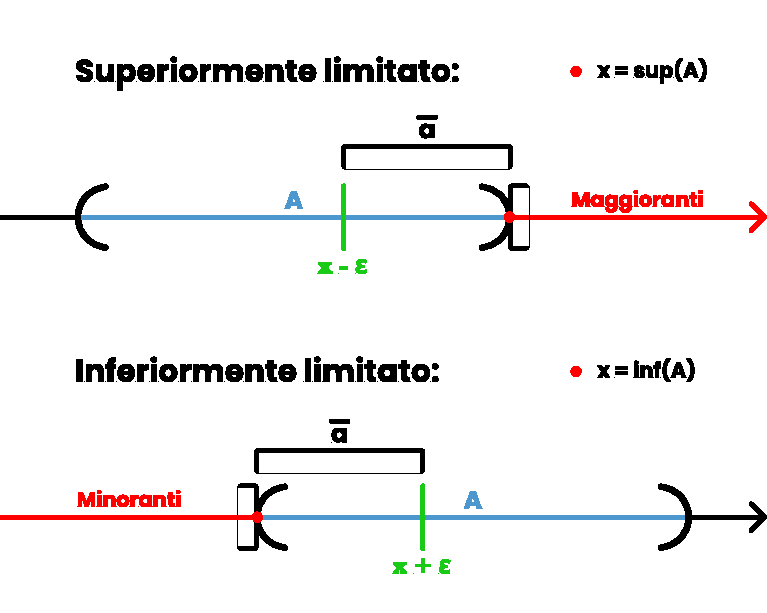
\includegraphics[width=8cm]{./images/infSupTheorem.pdf}
    \end{figure}
\end{center}

\noindent Dimostriamo ora l'implicazione ($\Rightarrow$) del punto a). Per ipotesi, sappiamo che $x = sup(A) \in \mathbb{R}$, allora $x \in M_A$ quindi $x \geq a \quad \forall a \in A$. In particolare, $x = min(M_A)$. \\
Sia $\varepsilon > 0$, allora $x - \varepsilon < x \implies x - \varepsilon \notin M_A$ (perché è più piccolo del minimo, cioè $x$). Dato che $\alpha \in M_A \underset{def}{\Longleftrightarrow} \alpha \geq a \quad \forall a \in A$, ma $\alpha \notin M_A$ (ovvero $\alpha \geq a \quad \forall a \in A$ è falsa). Possiamo dire che $\exists \Bar{a} \in A \ | \ \alpha < \Bar{a}$. Quindi $x - \varepsilon \notin M_A$ e posso scrivere che $\exists \Bar{a} \in A \ | \ x - \varepsilon < \Bar{a}$.\\
Dimostriamo ora la controimplicazione ($\Leftarrow$). Le ipotesi sono le seguenti:

\begin{enumerate}[label=\roman*)]
    \item $A$ è superiormente limitato;
    \item $x \geq a \quad \forall a \in A$;
    \item $\forall \varepsilon > 0, \exists \Bar{a} \in A \ | \ \Bar{a} > x - \varepsilon$
\end{enumerate}

\noindent La tesi da dimostrare è, invece, $x = sup(A)$. Per la seconda ipotesi (ii), capiamo che $x \in M_A$. Mentre dalla terza (iii) abbiamo che $x - \varepsilon \notin M_A \quad \forall \varepsilon > 0$ (cioè $x - \varepsilon$ non è un maggiorante). Segue quindi che:

\begin{equation}
    min(M_A) > x - \varepsilon \quad \forall \varepsilon > 0
    \label{eq:3}
\end{equation}

\noindent Sia ora $y = min(M_A)$, se fosse $y < x \implies \exists \Bar{\varepsilon} \ | \ y \leq x - \Bar{\varepsilon}$ che contraddice la (\ref{eq:3}). Pertanto, $y = min(M_A) \geq x$. Allora $x = min(M_A)$, ossia $x = sup(A)$.\\

\noindent Alla stessa maniera, dimostriamo ora il punto b). Partiamo dall'implicazione ($\Rightarrow$). Per ipotesi, sappiamo che $x = inf(A) \in \mathbb{R}$, allora $x \in m_A$ quindi $x \leq a \quad \forall a \in A$. In particolare, $x = max(m_A)$.\\
Sia $\varepsilon > 0$, allora $x + \varepsilon > x \implies x + \varepsilon \notin m_A$ (perché è più grande del massimo, cioè $x$). Dato che $\alpha \in m_A \underset{def}{\Longleftrightarrow} \alpha \leq a \quad \forall a \in A$, ma $\alpha \notin m_A$ (ovvero $\alpha \leq a \quad \forall a \in A$ è falsa). Possiamo dire che $\exists \Bar{a} \in A \ | \ \alpha > \Bar{a}$. Quindi $x + \varepsilon \notin m_A$ e posso scrivere che $\exists \Bar{a} \in A \ | \ x + \varepsilon > \Bar{a}$.\\
Dimostriamo ora la controimplicazione ($\Leftarrow$). Le ipotesi sono le seguenti:

\begin{enumerate}[label=\roman*)]
    \item $A$ è inferiormente limitato;
    \item $x \leq a \quad \forall a \in A$;
    \item $\forall \varepsilon > 0, \exists \Bar{a} \in A \ | \ \Bar{a} < x + \varepsilon$
\end{enumerate}

\noindent La tesi da dimostrare è, invece, che $x = inf(A)$. Per la seconda ipotesi (ii), capiamo che $x \in m_A$. Mentre dalla terza (iii) abbiamo che $x + \varepsilon \notin m_A \quad \forall \varepsilon > 0$ (cioè $x + \varepsilon$ non è un minorante). Segue quindi che:

\begin{equation}
    max(m_A) < x + \varepsilon \quad \forall \varepsilon > 0
    \label{eq:4}
\end{equation}

\noindent Sia ora $y = max(m_A)$, se fosse $y > x \implies \exists \Bar{\varepsilon} \ | \ y \geq x - \Bar{\varepsilon}$ che contraddice la (\ref{eq:4}). Pertanto, $y = max(m_A) \leq x$. Allora $x = max(m_A)$, ossia $x = inf(A)$.

\subsubsection{Esercizio 1}
\textbf{Sia $A \subseteq B \subseteq \mathbb{R}$. È vero che $supA \in B$? }

\noindent Dato che $B \subseteq \mathbb{R}$, se $supA \in B$, allora $supA \in \mathbb{R}$. Prendiamo allora $A = \mathbb{N}$ e $B = \mathbb{Z}$. Capiamo subito che $supA \notin \mathbb{R}$, dato che $A = \mathbb{N}$ non è superiormente limitato (e quindi $supA = + \infty$).\\
Ipotizziamo ora di avere due insiemi limitati come $A = (1,2)$ e $B = (0,1) \cup (1,2)$. Vediamo subito che $supA = 2 \notin B$, per cui anche qui non si verifica il caso $supA \in B$.\\

\noindent \textbf{Mostrare ora che $infA \geq infB$ e $supA \leq supB$.}

\noindent Partiamo dalla prima disuguaglianza e verifichiamo tutti i casi. Sia $A$ non inferiormente limitato (ovvero $infA = - \infty$). Ciò significa che anche $B$ non è inferiormente limitato (perché se lo fosse, anche $A$ dovrebbe necessariamente esserlo; $infB = - \infty$). Non essendo numeri reali, non possiamo dimostrare la disuguaglianza in questo caso.\\
\noindent Sia $A$ inferiormente limitato, allora $\exists \lambda_A \in \mathbb{R} \ | \ \lambda_A = infA$. Ora se $B$ non è inferiormente limitato, allora $infB = - \infty \notin \mathbb{R}$; se invece $B$ è inferiormente limitato, significa che $\exists \lambda_B \in \mathbb{R} \ | \ \lambda_B = infB$. Dato che $\lambda_B \leq b \quad \forall b \in B$ (ovvero $\lambda_B \in m_B$), ma ogni elemento di $A$ è sicuramente contenuto in $B$ perché $A \subseteq B$, abbiamo che $\lambda_B \in m_A$. Infine, essendo che $\lambda_A$ è il massimo dei minoranti di $A$, allora $\lambda_B \leq \lambda_A \implies infB \leq infA$. \\

\noindent Dimostriamo ora la seconda disuguaglianza e verifichiamo tutti i casi. Sia $A$ non superiormente limitato (ovvero $supA = + \infty$). Ciò significa che anche $B$ non è superiormente limitato (perché se lo fosse, anche $A$ dovrebbe necessariamente esserlo; $supB = - \infty$). Non essendo numeri reali, non possiamo dimostrare la disuguaglianza in questo caso. \\
\noindent Sia $A$ superiormente limitato, allora $\exists \lambda_A \in \mathbb{R} \ | \ \lambda_A = supA$. Ora se $B$ non è superiormente limitato, allora $supB = + \infty \notin \mathbb{R}$; se invece $B$ è superiormente limitato, significa che $\exists \lambda_B \in \mathbb{R} \ | \ \lambda_B = supB$. Dato che $\lambda_B \geq b \quad \forall b \in B$ (ovvero $\lambda_B \in M_B$), ma ogni elemento di $A$ è sicuramente contenuto in $B$ perché $A \subseteq B$, abbiamo che $\lambda_B \in M_A$. Infine, essendo che $\lambda_A$ è il minimo dei maggioranti di $A$, allora $\lambda_A \leq \lambda_B \implies supA \leq supB$.

\subsubsection{Esercizio 2}
\textbf{Sia $A \subseteq \mathbb{R}, A \neq \varnothing, -A \vcentcolon = \{ x \in \mathbb{R} \ | \ \exists y \in A \ per \ cui \ y = -x\}$. Provare che: $inf(-A) = -sup(A)$ e che $sup(-A) = -inf(A)$.} \\

\noindent Supponiamo che $A$ non sia inferiormente limitato, ossia che $\forall K \in \mathbb{R}, \exists a \in A \ | \ a < K$. Allora $(-A)$ non è superiormente limitato. Se, per contraddizione, lo fosse (superiormente limitato), allora $\exists H \in \mathbb{R} \ | \ b \leq H \quad \forall b \in (-A)$ (dove $H$ quindi è un maggiorante di $(-A)$). Siccome $b \in (-A) \iff b = -a \ per \ a \in A$, allora $-a \leq H \implies a \geq -H \quad \forall a \in A$. In altre parole, arriviamo ad una contraddizione perché abbiamo dimostrato che $A$ è inferiormente limitato, partendo dall'ipotesi che non lo fosse. Ciò significa che $-A$ non è superiormente limitato. Abbiamo quindi dimostrato che $infA = - \infty \implies sup(-A) = + \infty$.\\
Allo stesso modo, supponiamo che $A$ non sia superiormente limitato, ossia che $\forall K \in \mathbb{R}, \exists a \in A \ | \ a > K$. Allora $(-A)$ non è inferiormente limitato. Se, per contraddizione, lo fosse (inferiormente limitato), allora $\exists H \in \mathbb{R} \ | \ b \geq H \quad \forall b \in (-A)$ (dove $H$ quindi è un minorante di $(-A)$). Siccome $b \in (-A) \iff b = -a \ per \ a \in A$, allora $-a \geq H \implies a \leq -H \quad \forall a \in A$. In altre parole, arriviamo ad una contraddizione perché abbiamo dimostrato che $A$ è superiormente limitato, partendo dall'ipotesi che non lo fosse. Ciò significa che $-A$ non è inferiormente limitato. Abbiamo quindi dimostrato che $supA = + \infty \implies inf(-A) = - \infty$.\\
\noindent Sia ora $A$ inferiormente limitato, ovvero $\exists \lambda_A \in \mathbb{R} \ | \ \lambda_A = infA \quad (\lambda_A \leq a \quad \forall a \in A)$. Possiamo anche scrivere che $-\lambda_A \geq -a \quad \forall a \in A \implies -\lambda_A \geq b \quad \forall b \in (-A)$. Ciò però significa che $-\lambda_A$ è maggiorante di $-A$. Siccome $sup(-A) = minM_{(-A)} \leq -\lambda_A$, se si avesse $\Lambda_{(-A)} = sup(-A) < - \lambda_A$ (cioè solo strettamente più piccolo), allora $-a \leq \Lambda_{(-A)} < - \lambda_A \quad \forall a \in A$. Ora moltiplichiamo tutto per $-1$ ed otteniamo $a \geq - \Lambda_{(-A)} > \lambda_A \quad \forall a \in A$. Arriviamo così ad una contraddizione perché stiamo dicendo che $- \Lambda_{(-A)}$ è un minorante di $A$, maggiore di $\lambda_A = infA$ (ovvero il massimo dei minoranti). Ciò significa che la disuguaglianza di partenza era sbagliata. Quella corretta è: $- \Lambda_{(-A)} \leq \lambda_A \quad \forall a \in A \implies \Lambda_{(-A)} \geq - \lambda_A \quad \forall a \in A$. Dato che prima avevamo detto che $\Lambda_{(-A)} \leq - \lambda_A \quad \forall a \in A$, allora significa che $\Lambda_{(-A)} = - \lambda_A \implies sup(-A) = -infA$.\\
\noindent Sia ora $A$ superiormente limitato, ovvero $\exists \lambda_A \in \mathbb{R} \ | \ \lambda_A = supA \quad (\lambda_A \geq a \quad \forall a \in A)$. Possiamo anche scrivere che $-\lambda_A \leq -a \quad \forall a \in A \implies -\lambda_A \leq b \quad \forall b \in (-A)$. Ciò però significa che $-\lambda_A$ è minorante di $-A$. Siccome $inf(-A) = max(m_{(-A)}) \geq -\lambda_A$, se si avesse $\Lambda_{(-A)} = inf(-A) > -\lambda_A$ (cioè solo strettamente più piccolo), allora $- \lambda_A < \Lambda_{(-A)} \leq -a \quad \forall a \in A$. Ora moltiplichiamo tutto per $-1$ ed otteniamo $\lambda_A > - \Lambda_{(-A)} \geq a \quad \forall a \in A$. Arriviamo così ad una contraddizione perché stiamo dicendo che $-\Lambda_{(-A)}$ è un maggiorante di $A$, minore di $\lambda_A = supA$ (ovvero il minimo dei maggioranti). Ciò significa che la disuguaglianza di partenza è sbagliata. Quella corretta è: $- \Lambda_{(-A)} \geq \lambda_A \quad \forall a \in A \implies \Lambda_{(-A)} \leq - \lambda_A \quad \forall a \in A$. Dato che prima avevamo detto che $\Lambda_{(-A)} \geq - \lambda_A \quad \forall a \in A$, allora significa che $\Lambda_{(-A)} = - \lambda_A \implies inf(-A) = -supA$.

\subsubsection{Esercizio 3}
\textbf{Dati $A, B \subseteq \mathbb{R}$ con $ A, B \neq \varnothing$, sia $a \leq b \quad \forall a \in A, \forall b \in B$ e sia $A$ superiormente limitato e $B$ inferiormente limitato. Allora provare che $supA \leq infB$.}\\

\noindent Dalla consegna possiamo dire che $b \geq a \quad \forall a \in A \implies b \in M_A$. Dato che la precedente relazione è vera per ogni $b \in B$, allora possiamo dire che $B \subseteq M_A \implies b \geq minM_A = supA \quad \forall b \in B$. Essendo però che $supA \leq b$ dalla precedente disuguaglianza, allora $(supA) \in m_B \implies supA \leq max(m_B) = infB$. Infatti, presi due insiemi $A(-2, -1)$ e $B(0,1)$, si ha che $supA = -1 \leq 0 = infB$ (in questo esempio basterebbe addirittura semplicemente l'inclusione stretta $<$).

\subsubsection{Esercizio 4}
\textbf{Siano $A,B \neq \varnothing$ e $A, B \subseteq \mathbb{R}$ e sia $C = \{ a + b \ | \ a \in A, b \in B \}$.} \\

\noindent Provare che: 

\begin{enumerate}[label=\alph*)]
    \item se $A, B$ sono superiormente limitati, allora $supC = supA + supB$;
    \item se almeno uno tra $A$ e $B$ non è superiormente limitato, allora $supC = + \infty$;
    \item se $A, B$ sono inferiormente limitati, allora $infC = infA + infB$;
    \item se almeno uno tra $A$ e $B$ non è inferiormente limitato, allora $infC = - \infty$;
    \item in quale ipotesi per $A, B$ si ha che $supA + infB \leq supC = supA + supB$?
\end{enumerate}

\noindent \textbf{Punto a)}\\

\noindent Se $A, B$ sono superiormente limitati, significa che $\lambda = supA \in \mathbb{R} \implies a \leq \lambda \quad \forall a \in A$ e che $\mu = supB \in \mathbb{R} \implies b \leq \mu \quad \forall b \in B$. \\
Se ora prendiamo la prima disuguaglianza e sommiamo $b$, otteniamo $a + b \leq \lambda + b$. Dato però che $b \leq \mu \quad \forall b \in B$, allora possiamo scrivere: $a + b \leq \lambda + \mu \quad \forall a \in A, \forall b \in B$, che diventa $c \leq \lambda + \mu \quad \forall c \in C$. Ciò significa anche che $supC \leq \lambda + \mu$.\\
Sia ora $\varepsilon > 0$, sappiamo dal teorema della caratterizzazione di estremi inferiori e superiori reali che:

\begin{equation*}
    \exists a_1 \in A \ | \ a_1 > \lambda - \frac{\varepsilon}{2} \qquad \exists b_1 \in B \ | \ b_1 > \mu - \frac{\varepsilon}{2}
\end{equation*}

\noindent per cui:

\begin{equation*}
    c_1 \vcentcolon = a_1 + b_1 > \lambda - \frac{\varepsilon}{2} + \mu - \frac{\varepsilon}{2} \implies c_1 > \lambda + \mu - \varepsilon
\end{equation*}

\noindent In altre parole, $\forall \varepsilon > 0, \exists c_1 \in C \ | \ c_1 > \lambda + \mu - \varepsilon$. Sempre per il teorema della caratterizzazione di estremi inferiori e superiori reali, ciò significa che $supC = \lambda + \mu = supA + supB$.\\

\noindent \textbf{Punto b)}\\

\noindent Sia $A$ non superiormente limitato ($supA = + \infty$) e sia $b_0 \in B$. $\forall M > 0, \exists a_1 \in A \ | \ a_1 \geq M - b_0$. Ora possiamo spostare $b_0$ ed otteniamo $c_1 \vcentcolon = a_1 + b_0 \geq M \quad dove \ c_1 \in C$. Ciò significa che $C$ non ha maggioranti e quindi non è superiormente limitato, ovvero $supC = + \infty$.\\

\noindent \textbf{Punto c)}\\

\noindent Se $A, B$ sono inferiormente limitati, significa che $\lambda = infA \in \mathbb{R} \implies \lambda \leq a \quad \forall a \in A$ e che $\mu = infB \in \mathbb{R} \implies \mu \leq b \quad \forall b \in B$. \\
Se ora prendiamo la prima disuguaglianza e sommiamo $b$, otteniamo $a + b \geq \lambda + b$. Dato però che $b \geq \mu \quad \forall b \in B$, allora possiamo scrivere: $a + b \geq \lambda + \mu \quad \forall a \in A, \forall b \in B$, che diventa $c \geq \lambda + \mu \quad \forall c \in C$. Ciò significa che $infC \geq \lambda + \mu$. \\
Sia ora $\varepsilon > 0$, sappiamo dal teorema della caratterizzazione di estremi inferiori e superiori reali che:

\begin{equation*}
    \exists a_1 \in A \ | \ a_1 < \lambda + \frac{\varepsilon}{2} \qquad \exists b_1 \in B \ | \ b_1 < \mu + \frac{\varepsilon}{2}
\end{equation*}

\noindent per cui:

\begin{equation*}
    c_1 \vcentcolon = a_1 + b_1 < \lambda + \frac{\varepsilon}{2} + \mu + \frac{\varepsilon}{2} \implies c_1 < \lambda + \mu + \varepsilon
\end{equation*}

\noindent In altre parole, $\forall \varepsilon > 0, \exists c_1 \in C \ | \ c_1 < \lambda + \mu + \varepsilon$. Sempre per il teorema della caratterizzazione di estremi inferiori e superiori reali, ciò significa che $infC = \lambda + \mu = infA + infB$. \\

\noindent \textbf{Punto d)}\\

\noindent Sia $A$ non inferiormente limitato ($infA = - \infty$) e sia $b_0 \in B$. $\forall M < 0, \exists a_1 \in A \ | \ a_1 \leq M - b_0$. Ora possiamo spostare $b_0$ ed otteniamo $c_1 \vcentcolon = a_1 + b_0 \leq M \quad dove \ c_1 \in C$. Ciò significa che $C$ non ha minoranti e quindi non è inferiormente limitato, ovvero $supC = - \infty$.\\

\noindent \textbf{Punto e)}\\

\noindent Prendiamo $A, B$ superiormente limitati, dato che nel punto a) abbiamo dimostrato che $supC = supA + supB$. \\
Dato che $supA \in \mathbb{R}$, allora $supA + infB \leq supA + supB \implies infB \leq supB$. È quindi sufficiente avere che $(infB) \in \mathbb{R}$ per avere che $infB \leq supB$. Il punto e) risulta allora verificata per $A$ superiormente limitato e $B$ limitato.

\subsection{Disuguaglianza di Jacob Bernoulli}
\textbf{Teorema:} $x \in \mathbb{R}, x > -1$. Allora:

\begin{equation}
    (1 + x)^n \geq 1 + nx \qquad \forall n \in \mathbb{N}
    \label{eq:5}
\end{equation}

\subsubsection{Dimostrazione della disuguaglianza di Jacob Bernoulli}
\noindent\textbf{Passo base:} Fissiamo $p = 0$: 

\begin{equation*}
    (1 + x)^0 = 1 \geq 1 + 0x \implies 1 \geq 1 \implies passo \ base \ verificato
\end{equation*}

\noindent \textbf{Passo induttivo:} se $(1 + x)^n \geq 1 + nx$, allora $(1 + x)^{n+1} \geq 1 + (n+1)x$:

\begin{equation*}
    (1 + x)^{n+1} = (1+x)^n (1+x)
\end{equation*}

\noindent Dato che $(1 + x)^n \geq 1 + nx$, allora se moltiplichiamo a destra e a sinistra per $(1+x)$ otteniamo:

\begin{equation*}
    (1+x)^n (1+x) \geq (1+nx)(1+x)
\end{equation*}

\noindent Svolgendo i calcoli:

\begin{equation*}
    (1+x)^{n+1} \geq 1 + x + nx + nx^2
\end{equation*}

\begin{equation*}
    (1+x)^{n+1} \geq 1 + (n + 1)x + nx^2
\end{equation*}

\noindent Dato che $x \in \mathbb{R} \implies x^2 \geq 0$ e che $n \geq 0$, possiamo eliminare la quantità $nx^2$ e così il passo induttivo risulta verificato. A questo punto, non ci resta che applicare il principio di induzione per confermare la veridicità della (\ref{eq:5}).

\subsection{Binomio di Newton}
$\forall n \in \mathbb{N}, n \geq 1$ e $a, b \in \mathbb{R}$ si ha che:

\begin{equation}
    (a + b)^n = \sum_{k=0}^n \binom{n}{k} a^k b^{n-k}
    \label{eq:6}
\end{equation}

\subsubsection{Dimostrazione del binomio di Newton}
\noindent\textbf{Passo base:} Fissiamo $p = 1$: 

\begin{equation*}
    (a + b)^1 = a + b \qquad \sum_{k=0}^1 \binom{1}{k}a^k b^{1-k}=\binom{1}{0}a^0b^{1-0} + \binom{1}{1}a^1b^{1-1} = b+a \implies passo \ base \ verificato
\end{equation*}

\noindent\textbf{Passo induttivo:} 

\begin{equation*}
    se \ (a + b)^n = \sum_{k=0}^n \binom{n}{k} a^k b^{n-k}, \ allora \ (a+b)^{n+1} = \sum_{k=0}^{n+1} \binom{n + 1}{k} a^{k}b^{n+1-k}
\end{equation*}

\noindent Partiamo quindi dalla tesi:

\begin{equation*}
    (a+b)^{n+1} = (a + b)^n (a + b)
\end{equation*}

\noindent Per ipotesi induttiva possiamo dire che:

\begin{equation*}
    (a+b)^{n+1} = \left(\sum_{k=0}^n \binom{n}{k} a^k b^{n-k}\right)(a+b)
\end{equation*}

\noindent Ora applichiamo la proprietà distributiva:

\begin{equation*}
    (a+b)^{n+1} = \left(\sum_{k=0}^n \binom{n}{k} a^{k+1} b^{n-k} + \sum_{k=0}^n \binom{n}{k} a^k b^{n + 1-k}\right)
\end{equation*}

\noindent Per semplicità, chiamiamo la prima sommatoria $A$ e la seconda $B$. Ovvero:

\begin{equation*}
    A = \sum_{k=0}^n \binom{n}{k} a^{k+1} b^{n-k} \qquad B = \sum_{k=0}^n \binom{n}{k} a^k b^{n + 1-k}
\end{equation*}

\noindent Rinominiamo ora l'indice $k$ come $j = k + 1 \implies k = j - 1$. Quindi:

\begin{equation*}
    A = \sum_{j=1}^{n+1} \binom{n}{j-1} a^j b^{n-j+1} = \binom{n}{n} a^{n+1} + \sum_{j=1}^n \binom{n}{j-1} a^j b^{n+1-j} = a^{n+1} + \sum_{j=1}^n \binom{n}{j-1} a^j b^{n+1-j}
\end{equation*}

\noindent Prendiamo ora $B$ e riscriviamo la sommatoria in modo che parta da $1$:

\begin{equation*}
    B = \sum_{k=0}^n \binom{n}{k} a^k b^{n + 1-k} = \binom{n}{0} a^0 b^{n+1} + \sum_{k=1}^n \binom{n}{k} a^k b^{n + 1-k}
\end{equation*}

\noindent Possiamo quindi scrivere che: 

\begin{equation*}
    (a+b)^{n+1} = A + B = a^{n+1} + b^{n+1} + \sum_{l=1}^n \binom{n}{l-1} a^l b^{n+1-l} + \sum_{l=1}^n \binom{n}{l} a^l b^{n + 1-l}
\end{equation*}

\noindent Raccogliamo i fattori comuni, comprese le due sommatorie dato che entrambe vanno da $l = 1$ a $n$:

\begin{equation*}
    (a+b)^{n+1} = a^{n+1} + b^{n+1} + \sum_{l=1}^n \left(\binom{n}{l-1} + \binom{n}{l}\right) a^l b^{n+1-l}
\end{equation*}

\noindent Dalle proprietà del coefficiente binomiale, possiamo riscrivere: 

\begin{equation*}
    (a+b)^{n+1} = a^{n+1} + b^{n+1} + \sum_{l=1}^n \binom{n+1}{l} a^l b^{n+1-l}
\end{equation*}

\noindent Prendiamo ora $\dbinom{n+1}{l} a^l b^{n+1-l}$ e ipotizziamo che $l = n + 1$: 

\begin{equation*}
    \binom{n+1}{n+1} a^{n+1} b^{n+1-n-1} = a^{n+1}
\end{equation*}

\noindent Facendo la stessa cosa, ma con $l = 0$:

\begin{equation*}
    \binom{n+1}{0} a^0 b^{n+1-0} = b^{n+1}
\end{equation*}

\noindent Ne deriva che:

\begin{equation*}
    (a+b)^{n+1} = \sum_{l=0}^{n+1} \binom{n+1}{l} a^l b^{n+1-l}
\end{equation*}

\noindent La tesi è stata verificata, quindi possiamo concludere che il binomio di Newton è effettivamente vero $\forall n \in \mathbb{N}, n \geq 1$.
\newpage

\part{Applicazioni e limiti}
\section{Applicazione}
\begin{equation*}
    A \times B = \{ (a, b) \ | \ a \in A, b \in B \}
\end{equation*}

\noindent\textbf{NB!} Essendo $(a, b)$ una coppia ordinata, abbiamo che $(a, b) \neq (b, a)$. \\

\noindent Diciamo \textbf{applicazione} un sottoinsieme $\Phi \subseteq (A \times B)$ tale che $\forall (a_1, b_1), (a_2, b_2) \in \Phi$ si ha che $a_1 = a_2 \implies b_1 = b_2$. \\

\noindent Se dovessimo, invece, dare una definizione "operativa" di associazione: dati due insiemi $A, B$, diciamo applicazione una legge, che associa ad ogni elemento di $A$ un \textbf{unico} elemento di $B$.\\

\noindent \textbf{NB!} È quindi possibile che due punti di $A$ vanno nello stesso punto di $B$, ma non è possibile che lo stesso punto di $A$ vada in due punti di $B$. \\

\noindent Esempi di \textbf{non} applicazioni sono i seguenti (infatti allo stesso valore $a$ ci sono $b$ diversi):

\begin{figure}[h!]
    \centering
    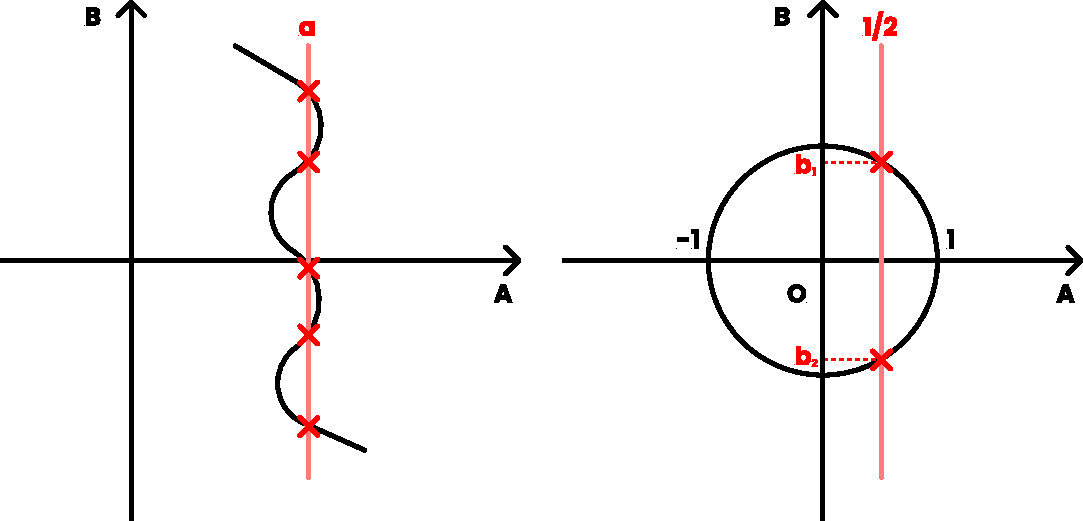
\includegraphics[width=10cm]{./images/notApplication.pdf}
\end{figure}

\noindent Un esempio di applicazione è invece:

\begin{figure}[h!]
    \centering
    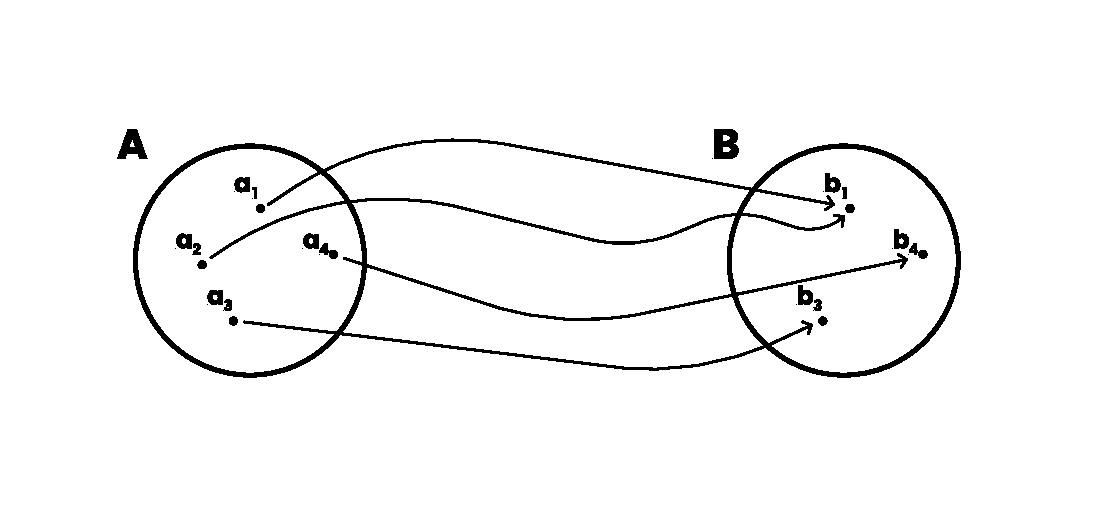
\includegraphics[width=11cm]{./images/application.pdf}
\end{figure}

\noindent Un'applicazione è formata da tre parti: due insiemi $A, B$ e una legge. Ad esempio: $\varphi: A \xrightarrow{} B$, è l'applicazione "phi" da $A$ a $B$, che ha come legge: $a \longmapsto \varphi(a) \ (\in B)$.\\

\noindent \textbf{Def:} $A = D(\varphi)$ è il dominio di $\varphi$, mentre $B = C(\varphi)$ è il codominio di $\varphi$.\\

\noindent \textbf{ES.} Le seguenti applicazioni sono tutte diverse, avendo insiemi diversi: 

\begin{equation*}
    f: \mathbb{R} \xrightarrow{} \mathbb{R} \quad x \longmapsto x^2 \qquad g: \mathbb{R} \xrightarrow{} [0, +\infty) \quad x \longmapsto x^2 \qquad h: [0, +\infty) \xrightarrow{} [0, +\infty) \quad x \longmapsto x^2
\end{equation*}

\noindent \textbf{Def:} L'\textbf{insieme immagine} di $\varphi$ è: $Imm(\varphi) = \{ b \in B \ | \ \exists a \in A \ per \ cui \ \varphi(a) = b \}$. Capiamo quindi che $Imm(\varphi) \subset B$. Un altro modo di scrivere questo insieme è: $Imm(\varphi) = \varphi(A)$. \\

\noindent Prendendo, ad esempio, l'applicazione $f$ scritta precedentemente, si può intuire che $Imm(f) = [0, +\infty)$, mentre $B = \mathbb{R}$, quindi $Imm(f) \subset B$. \\

\noindent \textbf{Def:} Sia $S \subset B$. Definisco controimmagine di $S$, secondo $\varphi$, l'insieme: 

\begin{equation*}
    \varphi^{-1} \vcentcolon = \{ a \in A \ | \ \varphi(a) \in S \} 
\end{equation*}

\noindent \textbf{NB!} $\varphi^{-1}$ non è il reciproco!\\

\noindent Presa, ad esempio, l'applicazione $f$ vista prima, possiamo capire che $\varphi(\{-1\})^{-1} = \varnothing$ (perché $x^2 \neq -1 \quad \forall x \in \mathbb{R}$) oppure $\varphi(\{1\})^{-1} = \{-1, 1\}$ (perché sia $x = -1$, che $x = 1$ elevati al quadrato mi danno $1$ come risultato). \\

\noindent \textbf{NB!} Dire $\{1, -1\}$ è diverso da dire $\{\pm 1\}$. Scrivere sempre e solo nel primo modo!

\subsection{Applicazione suriettiva, iniettiva e biettiva}
\textbf{Def:} Sia $\varphi: A \xrightarrow{} B$. Diremo che $\varphi$ è \textbf{suriettiva} se e solo se $Imm(f) = B$. Nell'esempio di prima, $f$ non è suriettiva, mentre $g$ e $h$ lo sono.\\

\noindent\textbf{Def:} Sia $\varphi: A \xrightarrow{} B$. Diremo che $\varphi$ è \textbf{iniettiva} se e solo se:

\begin{equation}
    \forall a_1, a_2 \in A \ con \ a_1 \neq a_2, \ si \ ha \ che \ \varphi(a_1) \neq \varphi(a_2)
    \label{eq:7}
\end{equation}

\noindent Equivalentemente, si può scrivere che: 

\begin{equation}
    \forall a_1, a_2 \in A \ | \ \varphi(a_1) = \varphi(a_2) \ si \ ha \ che \ a_1 = a_2
    \label{eq:8}
\end{equation}

\noindent Non è complicato dimostrare l'equivalenza di queste due definizioni. Basterà infatti procedere con una dimostrazione per contraddizione, che separi implicazione da controimplicazione. Partiamo quindi dall'implicazione ($\Rightarrow$), ovvero dalla definizione (\ref{eq:7}). Come ipotesi abbiamo che $a_1 \neq a_2$, mentre la tesi è che $\varphi(a_1) \neq \varphi(a_2)$. Negando quest'ultima (ovvero $\varphi(a_1) = \varphi(a_2)$), per la definizione di applicazione iniettiva, si ha che $a_1 = a_2$, che va però contro l'ipotesi iniziale. Arriviamo quindi ad una contraddizione. Ciò significa che se $a_1 \neq a_2$, allora per forza si ha che $\varphi(a_1) \neq \varphi(a_2)$. \\
Procediamo ora a verificare la controimplicazione ($\Leftarrow$; (\ref{eq:8})). L'ipotesi e la tesi sono rispettivamente $\varphi(a_1) = \varphi(a_2)$ e $a_1 = a_2$. Negando la tesi ($a_1 \neq a_2$), per definizione, abbiamo che $\varphi(a_1) \neq \varphi(a_2)$, il che va contro l'ipotesi iniziale. Per cui se $\varphi(a_1) = \varphi(a_2)$, allora per forza si ha che $a_1 = a_2$. \\

\noindent\textbf{Osservazione:} Sia $\varphi: A \xrightarrow{} B$:

\begin{enumerate}[label=\roman*)]
    \item $\varphi$ è suriettiva $\iff \forall b \in B, \exists a \in A \ | \ \varphi(a) = b$ (quindi $B \subseteq Imm(\varphi)$). Dato che per definizione $Imm(\varphi) \subseteq B \implies B = Imm(\varphi)$;
    \item $\forall b \in B, \exists !  a \in A \ | \ \varphi(a) = b$ (cioè ad ogni elemento del dominio corrisponde uno ed un solo elemento del codominio). In altre parole, è vero sia che $\varphi$ è suriettiva, sia che è iniettiva. Viene quindi detta \textbf{biettiva} o \textbf{biiezione} o \textbf{corrispondenza biunivoca}.
\end{enumerate}

\noindent Ritorniamo quindi un attimo agli esempi $f, g, h$. Consideriamo $f$: di certo non è suriettiva perché, ad esempio, $-1 \notin Imm(f)$. Ma è iniettiva? No, perché, ad esempio, $(1)^2 = 1$ e $(-1)^2 = 1$ (ci sono due punti distinti del dominio con la stessa immagine). \\
L'applicazione $g$, invece, è suriettiva ($Imm(g) = B$), ma non è iniettiva perché $\forall \alpha > 0, g^{-1}(\{\alpha\}) = \{-\sqrt{\alpha}, \sqrt{\alpha}\}$.\\
Infine, $h$ è sia suriettiva, sia iniettiva infatti $\forall \alpha > 0, g^{-1}(\{\alpha\}) = \{\sqrt{\alpha}\}$. Proprio per questo motivo, $h$ è biettiva.

\subsubsection{Corrispondenza biunivoca tra l'insieme dei numeri pari ed $\mathbb{N}$}
Siano $P = \{2m \ | \ m \in \mathbb{N}\}$ e $\mathbb{N}$. La nostra tesi è che esiste una corrispondenza biunivoca tra i due insiemi, in simboli:

\begin{equation*}
    P \overset{\Psi}{\longrightarrow} \mathbb{N}
\end{equation*}

\noindent\textbf{NB!} Cantor ha dimostrato che gli insiemi $\mathbb{N}, \mathbb{Z}, \mathbb{Q}$ sono tali che si può costruire tra loro una corrispondenza biunivoca. Sono infatti degli \textbf{insiemi numerabili}. Al contrario, $\mathbb{R}$ e $\mathbb{C}$ non sono numerabili.\\

\noindent Consideriamo quindi la seguente applicazione come biettiva: 

\begin{equation*}
    \Psi: \mathbb{N} \xrightarrow{} P \qquad m \longmapsto 2m \qquad \qquad con \ P \subsetneq \mathbb{N}
\end{equation*}

\noindent\textbf{Suriettività:} Sia $2m \in P$, la nostra tesi è che $\exists n \in \mathbb{N} \ | \ \Psi(n) = 2m$. Per definizione $\Psi(m) = 2m$, ma dato che dalla riga precedente abbiamo detto che $\Psi(n) = 2m$, allora $n = m$. Per questo motivo, $\Psi$ è suriettiva.\\

\noindent\textbf{Iniettività:} Siano $m_1 \neq m_2$ con $m_1, m_2 \in \mathbb{N}$. La nostra tesi è che $\Psi(m_1) \neq \Psi(m_2)$, dimostriamola per contraddizione! Supponiamo quindi che $\Psi(m_1) = \Psi(m_2)$. Ciò significa che se $\Psi(m_1) = 2m_1$ e $\Psi(m_2) = 2m_2$, allora $2m_1 = 2m_2$. Svolgendo un po' di conti:

\begin{equation*}
    2m_1 - 2m_2 = 0 \implies 2(m_1-m_2) = 0 \implies m_1 - m_2 = 0 \implies m_1 = m_2
\end{equation*}

\noindent Arriviamo quindi proprio ad una contraddizione, dato che per ipotesi $m_1 \neq m_2$, ne deriva che $\Psi(m_1) \neq \Psi(m_2)$. Quindi $\Psi$ è iniettiva.

\subsubsection{Paradosso del Grand Hotel di Hilbert}
Hilbert immagina un hotel con infinite stanze, tutte occupate, e afferma che qualsiasi sia il numero di altri ospiti che sopraggiungano, sarà sempre possibile ospitarli tutti, anche se il loro numero è infinito, purché numerabile.\\
Infatti, quando arrivano infiniti nuovi ospiti basta spostare ogni ospite nella stanza con numero doppio rispetto a quello attuale, lasciando così ai nuovi ospiti tutte le camere con i numeri dispari, che sono essi stessi infiniti, risolvendo dunque il problema. Gli ospiti sono tutti dunque sistemati, benché l'albergo fosse pieno.

\subsection{Somma, prodotto, rapporto e composizione di applicazioni}
\textbf{Def:} $\varphi: A \xrightarrow{} \mathbb{R}, \Psi: B \xrightarrow{} \mathbb{R}$, definiamo l'applicazione somma di $\varphi + \Psi$: 

\begin{equation*}
    (\varphi + \Psi): A \cap B \xrightarrow{} \mathbb{R} \qquad a \longmapsto \varphi(a) + \Psi(a)
\end{equation*}

\noindent Dato che il dominio è $A \cap B$, si capisce che nella somma, l'elemento $a$ deve appartenere sia ad $A$, che a $B$. \\

\noindent Dato che la somma in $\mathbb{R}$ è commutativa, allora: $(\varphi + \Psi) = (\Psi + \varphi)$ perché $\varphi(a) + \Psi(a) = \Psi(a) + \varphi(a)$.\\

\noindent\textbf{ES.} Dati $\varphi: [0, + \infty) \xrightarrow{} \mathbb{R} \quad x \longmapsto \sqrt{x}$ e $\Psi: \mathbb{R} \xrightarrow{} \mathbb{R} \quad x \longmapsto 2x$, allora $\varphi + \Psi: x \longmapsto \sqrt{x} + 2x \quad D(\varphi + \Psi) = [0, +\infty) \cap \mathbb{R} = [0, +\infty)$. \\

\noindent\textbf{Def:} Chiamiamo \textbf{grafico} di $\varphi: A \xrightarrow{} B$, l'insieme:
\begin{equation*}
    \Gamma(\varphi) = \mathcal{G}(\varphi) = \{(a, \varphi(a)) \ | \ a \in A\} \quad dove \ \varphi(a) \in B
\end{equation*}

\noindent\textbf{NB!} $\Gamma(\varphi) = \mathcal{G}(\varphi)$ è un sottoinsieme del prodotto cartesiano $C(A\times B)$. \\

\noindent Sia $f: A \xrightarrow{} \mathbb{R}$ e $c: \mathbb{R} \xrightarrow{} \mathbb{R} \quad x \longmapsto c$. \\
\noindent Prendiamo ora $D(f + c) = D(f) \cap D(c) = A \cap \mathbb{R} = A$. \\
\noindent Possiamo capire semplicemente che preso il grafico di $f$ e quello di $f + c$, essi variano solo per la seconda componente:
\begin{gather*}
    \mathcal{G}(f + c) = \{(a, f(a) + c) \ | \ a \in A\}\\
    \mathcal{G}(f) = \{(a, f(a)) \ | \ a \in A\}
\end{gather*}

\noindent Questa componente $c$ permette di traslare il grafico. In particolare:

\begin{itemize}
    \item se $c > 0$, allora $f(a) < f(a) + c$ e quindi l'applicazione trasla rigidamente verso l'alto;
    \item se $c < 0$, allora $f(a) > f(a) + c$ e quindi l'applicazione trasla rigidamente verso il basso.
\end{itemize}

\noindent\textbf{NB!} $c: \mathbb{R} \xrightarrow{} \mathbb{R} \quad x \longmapsto c$ viene definita \textbf{applicazione costante} perché va da $\mathbb{R} \xrightarrow{} \mathbb{R}$ e ad ogni $x$ associa lo stesso valore $c$. Per questo motivo, non è né iniettiva (perché ogni punto di $\mathbb{R}$ finisce nella stessa immagine), né suriettiva (perché l'immagine è solo $c$, mentre il codominio è tutto $\mathbb{R}$).\\

\noindent Sia $f: D(f) \xrightarrow{} \mathbb{R} \quad x \longmapsto f(x)$, allora se prendiamo $\mathcal{G}(bf): (bf): D(f) \xrightarrow{} \mathbb{R} \quad x \longmapsto bf(x) \quad con \ b \in \mathbb{R}$, esso dipenderà proprio da $b$. In particolare: 

\begin{itemize}
    \item se $b = 1$, ovviamente il grafico rimane uguale;
    \item se $b > 0 \wedge b \neq 1$, viene applicato un effetto di \textbf{deformazione} all'applicazione;
    \item se $b = -1$ il grafico viene \textbf{ribaltato};
    \item se $b < 0 \wedge b \neq -1$, viene applicato un effetto di \textbf{deformazione} all'applicazione dovuto a $|b|$ ed un effetto di \textbf{ribaltamento} dovuto al fatto che $b < 0$.
\end{itemize}

\noindent Sia ora $f: A \subset \mathbb{R} \xrightarrow{} \mathbb{R} \quad x \longmapsto f(x)$ e $g: C \subset \mathbb{R} \xrightarrow{} \mathbb{R} \quad x \longmapsto f(x + c)$, dove $c \in \mathbb{R}$ ed è fissato. Notiamo che in $g$ stanno avvenendo due operazioni: prima trasliamo $x$ in $x + c$ e poi applichiamo il risultato ad $f$. Il dominio di $g$ sarà quindi: $C = D(g) = \{x \in \mathbb{R} \ | \ (x + c) \in D(f) = A\}$. Ciò significa quindi che $x+c = a$ dove $a \in A$. In particolare, si ha che $A = \{x \in \mathbb{R} \ | \ \exists a \in A \ tale \ che \ x = a -c\}$. In altre parole, stiamo traslando il dominio $D(f)$ di una certa quantità $c$. \\

\noindent\textbf{ES.} Sia $A = [-1, 1] \quad c = 2$, allora $C = \{x \in \mathbb{R} \ | \ \exists a \in [-1, 1] \ tale \  che \ x = a-2\}$. Quindi $C = [-3, -1]$.\\

\noindent\textbf{NB!} A volte si trova anche la notazione $C = \{a-b \ | \ a \in A, b \in B\} = \vcentcolon A - B$, dove, secondo l'esempio di prima, $B = \{c\}$.\\

\noindent\textbf{Def:} Dati $A, B$ con $A \cap B \neq \varnothing$. Siano $\varphi: A \xrightarrow{} \mathbb{R}$ e $\Psi: B \xrightarrow{} \mathbb{R}$. L'applicazione prodotto è:
\begin{gather*}
    \Psi \cdot \varphi: (A \cap B) \xrightarrow{} \mathbb{R}\\
    a \longmapsto \Psi(a) \cdot \varphi(a)
\end{gather*}

\noindent Come nel caso della somma tra due applicazioni, si ha che $\Psi \cdot \varphi = \varphi \cdot \Psi$ perché il prodotto $\Psi(a) \cdot \varphi(a) = \varphi(a) \cdot \Psi(a)$.\\

\noindent\textbf{Def:} Dati $A, B$ con $A \cap B \neq \varnothing$. Siano $\varphi: A \xrightarrow{} \mathbb{R}$ e $\Psi: B \xrightarrow{} \mathbb{R}$. L'applicazione rapporto è:
\begin{gather*}
    \frac{\Psi}{\varphi}: (A \cap B) \cap \{a \in A \ | \ \varphi(a) \neq 0 \} \xrightarrow{} \mathbb{R} \\
    a \longmapsto \frac{\Psi(a)}{\varphi(a)}
\end{gather*}

\noindent\textbf{NB!} La condizione aggiunta rispetto alla somma e al prodotto serve a specificare che il denominatore dev'essere non nullo. \\

\noindent\textbf{NB!} Definiamo l'insieme degli zeri di un'applicazione $f$: $z_f = \{a \in D(f) \ | \ f(a) = 0\}$. Allora dire che $\dfrac{\Psi}{\raisebox{0.2ex}{$\varphi$}} \neq \dfrac{\raisebox{0.4ex}{$\varphi$}}{\raisebox{-0.3ex}{$\Psi$}}$, infatti:

\begin{equation*}
    D\left(\frac{\Psi}{\varphi}\right) - z_\varphi \quad D\left(\frac{\raisebox{0.4ex}{$\varphi$}}{\raisebox{-0.3ex}{$\Psi$}}\right) - z_\Psi \implies D\left(\frac{\Psi}{\varphi}\right) \neq D\left(\frac{\raisebox{0.4ex}{$\varphi$}}{\raisebox{-0.3ex}{$\Psi$}}\right)
\end{equation*}

\section{Topologia della retta reale}
\textbf{Def:} Sia $x \in \mathbb{R}$ e sia $\varepsilon > 0$. Diremo \textbf{intorno} di centro $x_0$ e raggio $\delta$ l'intervallo: 

\begin{equation*}
    D(x_0, \delta) \vcentcolon = \{x\in\mathbb{R} \ | \ |x - x_0| < \delta\} \vcentcolon = (x_0 - \delta, x_0 + \delta)
\end{equation*}

\noindent\textbf{NB!} Viene anche detto \textbf{intorno circolare}.\\

\noindent\textbf{Intorno di $+\infty$ - Def:} Ogni intervallo del tipo $(a, + \infty)$ per $a \in \mathbb{R}$:

\begin{equation*}
    \{x\in\mathbb{R} \ | \ x > a\}
\end{equation*}

\noindent ovvero tutti gli intervalli non superiormente limitati.\\

\noindent\textbf{Intorno di $-\infty$ - Def:}  Ogni intervallo del tipo $(- \infty, a)$ per $a \in \mathbb{R}$:

\begin{equation*}
    \{x\in\mathbb{R} \ | \ x < a\}
\end{equation*}

\noindent È facile capire quindi che in questi insiemi si ha:
\begin{gather*}
    sup((a, +\infty)) = +\infty \qquad inf((a, +\infty)) = a \\
    sup((-\infty, a)) = a \qquad inf((-\infty, a)) = - \infty
\end{gather*}

\noindent Prima di continuare con la spiegazione, definiamo l'insieme $\widetilde{\mathbb{R}} = \mathbb{R} \cup \{-\infty, +\infty\}$, dove $\widetilde{\mathbb{R}}$ si legge \textbf{$\mathbb{R}$ esteso}. In altre parole, se $x_0 \in \widetilde{\mathbb{R}}$, allora o $x_0 \in \mathbb{R}$ o $x_0 = +\infty$ oppure $x_0 = - \infty$.\\

\noindent \textbf{Def:} Sia $A \subset \mathbb{R}$ con $A \neq \varnothing$. Sia ora $x_0 \in \mathbb{R}$. Diremo che $x_0$ è \textbf{punto di accumulazione} per $A$ se e solo se:

\begin{equation*}
    \forall \delta > 0 \ si \ ha \ che \ (D(x_0, \delta) \cap A) - \{x_0\} \neq \varnothing
\end{equation*}

\noindent In altre parole, significa che esistono punti di $A$, diversi da $x_0$, arbitrariamente vicini a $x_0$. \\

\noindent\textbf{NB!} $D(x_0, \delta)$ è un intorno circolare di $x_0$.\\

\noindent\textbf{NB!} $x_0 \in \mathbb{R}$, ma non deve per forza appartenere ad $A$ per essere un suo punto di accumulazione.

\subsection{Esercizio 5}
\textbf{Sia $A = (1, 2) \cup \{3\}$. Quali sono i punti di accumulazione reali di $A$?}

\noindent Ipotizziamo che $x < 1$. Prendendo quindi un $\delta > 0$, otteniamo un intorno $I = (x - \delta, x + \delta) \cap A$. In particolare, questo intorno $I$ sarà composto da tutti i numeri compresi tra $1$ e $x + \delta$. Questo però non vale per ogni $\delta > 0$. Infatti, se prendiamo $\delta < \Delta = 1 - x$ (dove $\Delta$ rappresenta la distanza tra $1$ e $x$), si ha che $I = \varnothing$. Ciò significa che se $x < 1$, allora $x$ non è un punto di accumulazione. 
Si può anche osservare quanto spiegato qui sopra dalla prima immagine della prossima pagina.

\noindent Sia ora $x = 1$ (come detto precedentemente, anche se $1 \notin A$, non significa che esso non possa essere punto di accumulazione per $A$). Allora possiamo prendere un $\delta > 0$, tale che $J = (1 - \delta, 1 + \delta) \cap A \neq \varnothing$. Dato che quest'ultima relazione deve essere verificata per ogni $\delta > 0$, dobbiamo procedere con tutti i casi. Di seguito, troviamo le immagini raffiguranti cosa succede in ogni caso e un sistema finale che riassume tutti i conti.

\begin{figure}[!h]
    \centering
    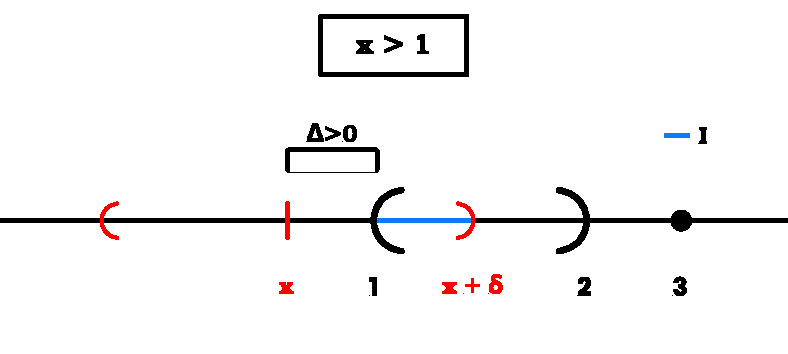
\includegraphics[width=12cm]{./images/AccPoints1.pdf}
\end{figure}

\begin{figure}[!h]
    \centering
    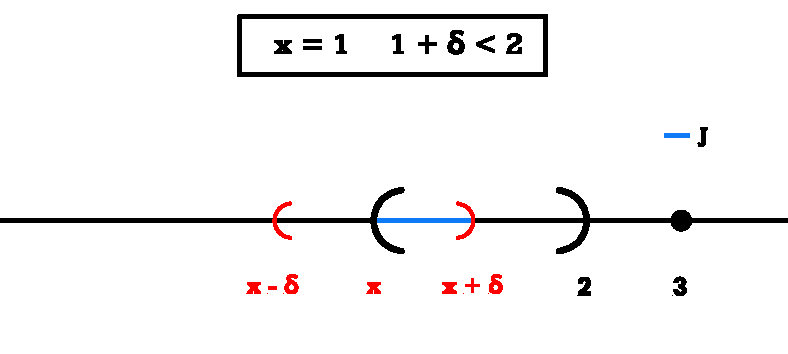
\includegraphics[width=7cm]{./images/AccPoints2.pdf}\hfill
    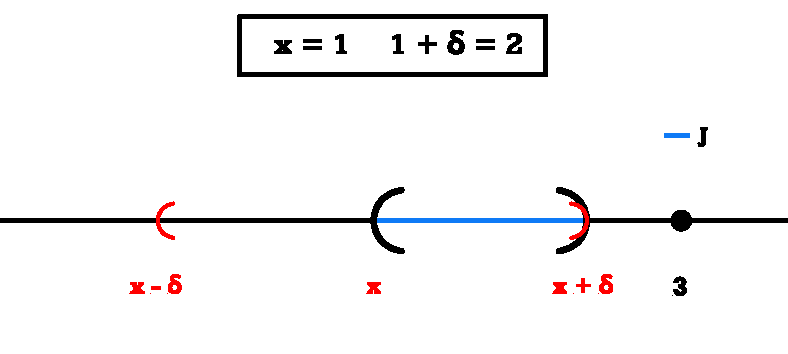
\includegraphics[width=7cm]{./images/AccPoints3.pdf}
\end{figure}

\begin{figure}[!h]
    \centering
    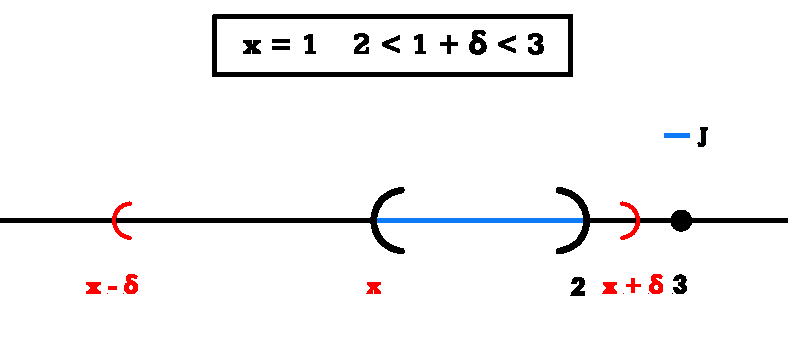
\includegraphics[width=7cm]{./images/AccPoints4.pdf}\hfill
    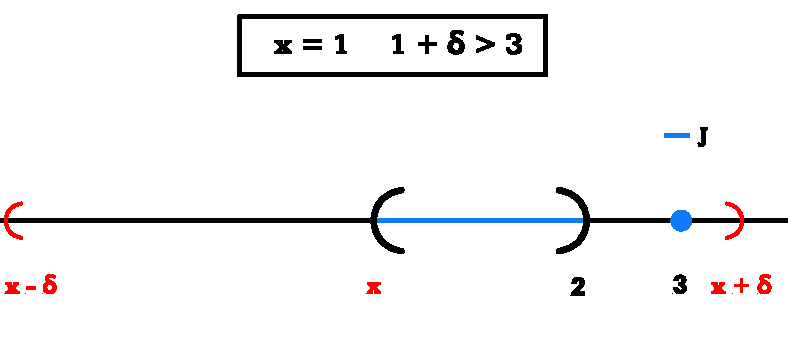
\includegraphics[width=7cm]{./images/AccPoints5.pdf}
\end{figure}

\begin{equation*}
    J =
    \begin{cases}
    (1, 1 + \delta) \quad se \ \delta < 1 \\
    (1, 2) \quad se \ \delta = 1 \\
    (1, 2) \quad se \ 1 < \delta < 2 \\
    (1, 2) \quad se \ \delta = 2 \\
    A \quad se \ \delta > 2
\end{cases}
\end{equation*}

\noindent Dato che per la definizione di punto di accumulazione, dall'intersezione $D(x_0,\delta) \cap A$ è necessario togliere $x_0$, togliendo $x = 1$ da $J$, notiamo che esso rimane non vuoto. Possiamo quindi concludere che $1$ è punto di accumulazione per l'insieme $A$.

\subsection{Esercizio 6}
\textbf{Verificare che $x = 2$ è punto di accumulazione.}

\noindent Procediamo allo stesso modo di prima:

\begin{equation*}
    J = \begin{cases}
        A \quad se \ 2 - \delta < 1 \implies \delta > 1 \\
        (2-\delta, 2) \quad se \ 2 - \delta > 1 \implies \delta < 1 \\
        A \quad se \ \delta = 1
    \end{cases}
\end{equation*}

\noindent In generale, togliendo $x = 2$ da $J$ notiamo che esso rimane non vuoto. Possiamo quindi concludere che $2$ è punto di accumulazione per l'insieme $A$. Di seguito, è possibile verificare graficamente perché abbiamo ottenuto questi risultati. 

\begin{figure}[!h]
    \centering
    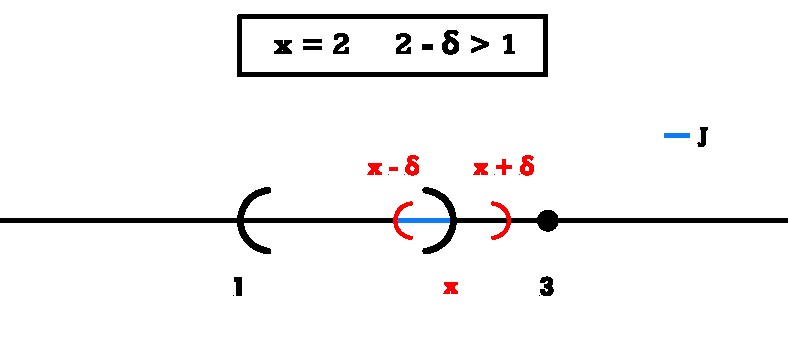
\includegraphics[width=7cm]{./images/AccPoints6.pdf}\hfill
    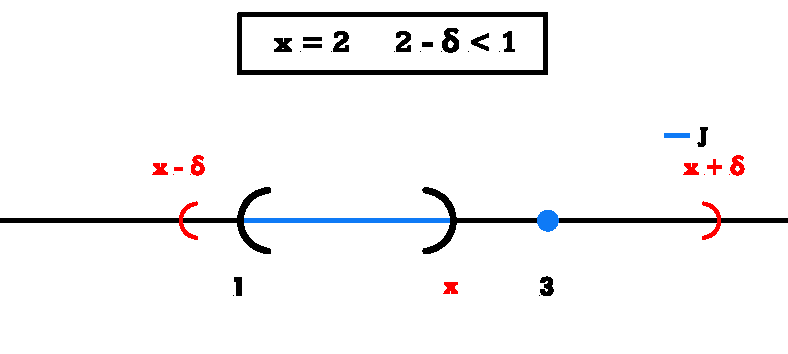
\includegraphics[width=7cm]{./images/AccPoints7.pdf}
\end{figure}

\begin{figure}[!h]
    \centering
    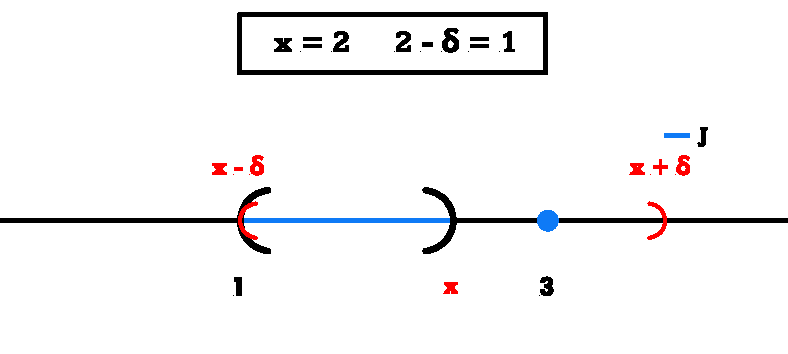
\includegraphics[width=12cm]{./images/AccPoints8.pdf}
\end{figure}

\subsection{Esercizio 7}
\textbf{Verificare che qualsiasi $x_0 \in (1, 2)$ è punto di accumulazione per $A$.}

\noindent Semplicemente, essendo $x_0 \in (1, 2)$, ciò significa che $1 < x_0 < 2$. A livello visivo:

\begin{figure}[!h]
    \centering
    $\vcenter{\hbox{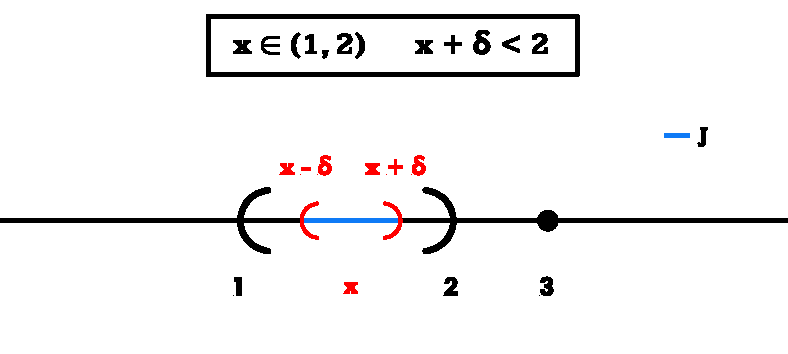
\includegraphics[width=5cm]{./images/AccPoints9.pdf}}}$\hfill
    $\vcenter{\hbox{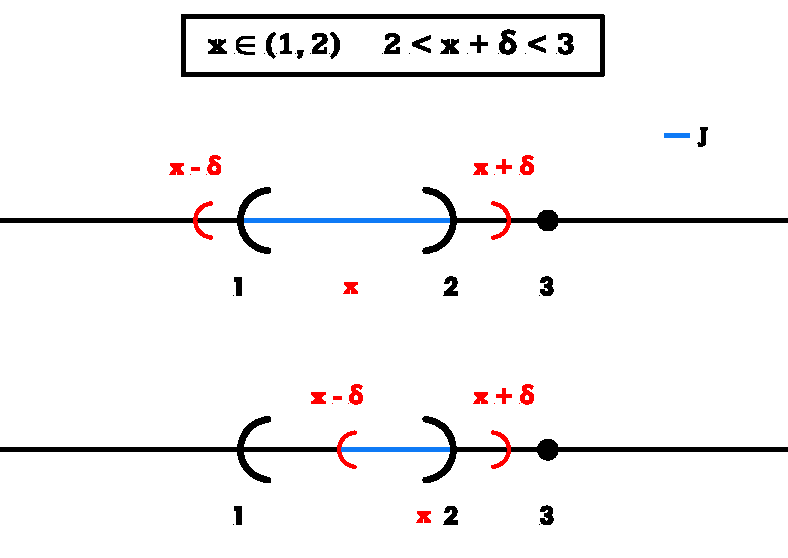
\includegraphics[width=5cm]{./images/AccPoints10.pdf}}}$\hfill
    $\vcenter{\hbox{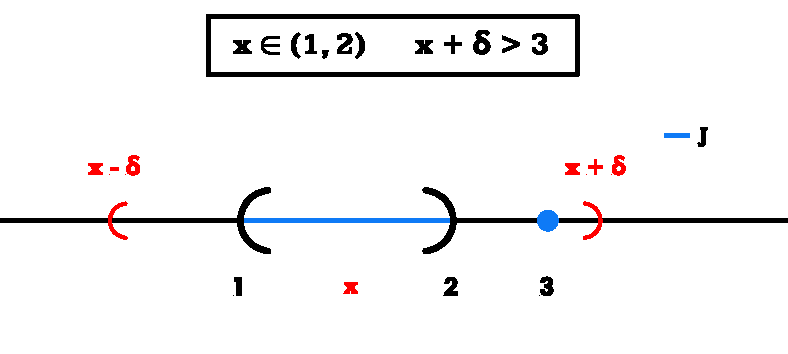
\includegraphics[width=5cm]{./images/AccPoints11.pdf}}}$
\end{figure}

\noindent Quindi:

\begin{itemize}
    \item se $x_0 + \delta < 2$, allora $J = (x_0 - \delta, x_0 + \delta)$;
    \item se $2 < x_0 + \delta < 3$, allora:
    \begin{itemize}
        \item se $x_0 - \delta > 1$, allora $J = (x_0 - \delta, 2)$;
        \item se $x_0 - \delta < 1$, allora $J = (1, 2)$
    \end{itemize}
    \item se $x_0 + \delta > 3$, allora $J = A$;
    \item se $x_0 + \delta = 2$, allora:
    \begin{itemize}
        \item se $x_0 - \delta \leq 1$, allora $J = (1, 2)$;
        \item se $x_0 - \delta > 1$, allora $J = (x_0 - \delta, 2)$.
    \end{itemize}
\end{itemize}

\noindent Togliendo ora $x_0$ da $J$, quest'ultimo rimane non vuoto. Per cui possiamo concludere che qualsiasi $x_0 \in (1, 2)$ è un punto di accumulazione.

\subsection{Esercizio 8}
\textbf{Verificare che qualsiasi $x > 2 \wedge x \neq 3$, $x$ non è punto di accumulazione per $A$.}

\noindent Per farlo basta trovare un unico caso per cui vale che $J = ((x_0 - \delta, x_0 + \delta) \cap A) - \{x_0\} = \varnothing$. Prendendo quindi $x_0 + \delta < 3$ oppure prendendo un numero $x > 3$ e un $\delta < \Delta = x - 3$ (dove $\Delta$ è la distanza tra $x$ e $3$), si ha che non vi è nessuna intersezione con l'insieme A e quindi $J = \varnothing$. Per cui possiamo concludere che $3$ non è un punto di accumulazione per $A$. Graficamente:

\begin{figure}[!h]
    \centering
    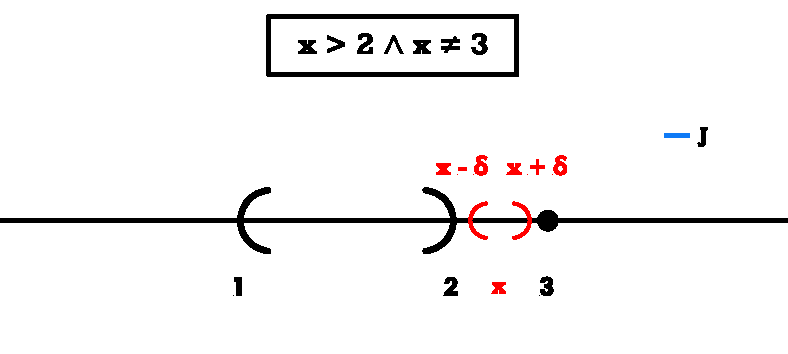
\includegraphics[width=12cm]{./images/AccPoints12.pdf}
\end{figure}

\subsection{Esercizio 9}
\textbf{Dimostrare che $x_0 = 3$ non è punto di accumulazione per $A$.}

\noindent Dire che $x_0 = 3$ non è punto di accumulazione per $A$, significa che $\exists \Bar{\delta} > 0 \ | \ ((3 - \Bar{\delta}, 3 + \Bar{\delta}) \cap A) - \{3\} = \varnothing$. \\
Se prendiamo un $\Bar{\delta} > 0$ tale che $3 - \Bar{\delta} > 2 \implies \Bar{\delta} < 1$ avremo che $((3 - \Bar{\delta}, 3 + \Bar{\delta}) \cap A) - \{3\} = \varnothing$. Si verifica infatti con, ad esempio, $\Bar{\delta} = \dfrac{1}{2}$. Per questo motivo, possiamo concludere che $3$ non è un punto di accumulazione per $A$.\\

\subsection{Esercizio 10}
\textbf{Sia $B = [1, 2] \cup \{3\}$, provare che i punti di accumulazione di $B$ sono tutti e soli quelli dell'insieme $[1,2]$.}

\noindent Procediamo per casi: 

\begin{itemize}
    \item Se $x < 1$, allora, come per il primo esempio su questa tipologia di esercizi, $x$ non è punto di accumulazione perché preso un $\delta < \Delta = 1 - x$ (dove $\Delta$ rappresenta la distanza tra $1$ e $x$), l'intersezione $J = \varnothing$;
    \item se $x = 1$, allora:
    \begin{itemize}
        \item se $1 < 1 + \delta < 2 \implies 0 < \delta < 1$, avremo che $J = [1, x_0 + \delta)$;
        \item se $1 + \delta > 2 \implies \delta > 1$, avremo che $J = [1, 2]$;
        \item se $1 + \delta = 2 \implies \delta = 1$, avremo che $J = [1, 2)$;
    \end{itemize}
    \item se $1 < x < 2$, allora:
    \begin{itemize}
        \item se $1 + \delta < 2 \implies \delta < 1$, allora $J = (1 - \delta, 1 + \delta)$;
        \item se $1 + \delta = 2 \implies \delta = 1$, allora $J = (1 - \delta, 2)$;
        \item se $1 + \delta > 2 \implies \delta > 1$, allora:
        \begin{itemize}
            \item $x_0 - \delta > \Delta = x - 1$, allora $J = (x_0 - \delta, 2]$;
            \item se $x_0 - \delta < \Delta = x - 1$, allora $J = [1, 2]$;
            \item se $x_0 - \delta < \Delta = x - 1$, allora $J = (1, 2]$
        \end{itemize}
    \end{itemize}
    \item se $x = 2$, allora: 
    \begin{itemize}
        \item se $x_0 - \delta > 1$, allora $J = (x_0 - \delta, 2]$;
        \item se $x_0 - \delta < 1$, allora $J = A$;
        \item se $x_0 - \delta = 1$, allora $J = (1, 2]$;
    \end{itemize}
    \item se $x > 2$, allora, come per $x < 1$, preso $\delta > \Delta = x - 2$, allora $J = \varnothing$.
\end{itemize}

\noindent Notiamo come in tutti per qualsiasi $x$ tale che $x < 1$ o $x > 2$, essa non è punto di accumulazione di $a$, mentre $x \in [1, 2]$ è un punto di accumulazione, come volevasi dimostrare.\\

\subsection{Esercizio 11}
\textbf{Sia $I = (a, b)$, $J = [a, b)$, $K = (a, b]$ e $L = [a, b]$. Provare che i punti di accumulazione di $I, J, K, L$ sono tutti e soli i punti $[a, b]$.}

\noindent Ancora una volta procediamo per casi:

\begin{itemize}
    \item se $x < a$ e $\delta < \Delta = 1 - x$, allora qualsiasi sia l'insieme che stiamo valutando, esso sarà vuoto;
    \item se $x = a$, allora l'insieme derivante dall'intersezione sarà pari a $[a, x_0 + \delta)$ (oppure a $[a, b]$, se $x_0 + \delta > b$);
    \item se $a < x < b$, allora:
    \begin{itemize}
        \item se $x_0 + \delta < b$, allora:
        \begin{itemize}
            \item se $x_0 - \delta < a$, allora l'insieme derivante dall'intersezione sarà pari a $[a, x_0 + \delta)$;
            \item se $x_0 - \delta > a$, allora l'insieme derivante dall'intersezione sarà apri a $(x_0 - \delta, x_0 + \delta)$;
        \end{itemize}
        \item se $x_0 + \delta > b$, allora:
        \begin{itemize}
            \item se $x_0 - \delta < a$, allora l'insieme derivante dall'intersezione sarà pari a $[a, b]$;
            \item se $x_0 - \delta > a$, allora l'insieme derivante dall'intersezione sarà pari a $(x_0 - \delta, b]$;
        \end{itemize}
    \end{itemize}
    \item se $x = b$, allora l'insieme derivante dall'intersezione sarà pari a $(x_0 - \delta, b]$ (oppure a $[a, b]$, se $x_0 - \delta < a$);
    \item se $x > b$, allora basterà prendere un $\delta > \Delta = x - b$ per far in modo che qualsiasi sia l'insieme considerato, l'intersezione prodotta sia un insieme vuoto.
\end{itemize}

\noindent Notiamo quindi che tutti i valori di $x < a \vee x > b$ non sono punti di accumulazione perché l'intersezione prodotta è pari ad un insieme vuoto; mentre i punti $a \leq x \leq b$ sono tutti punti di accumulazione per qualsiasi dei quattro insiemi considerati (a seconda dell'insieme considerato, le parentesi quadre della lista qui sopra potrebbero essere delle parentesi tonde).\\

\noindent\textbf{Def:} Chiamiamo \textbf{punti isolati} i punti $x_0 \in \mathbb{R}$ dell'insieme $A \subset \mathbb{R}$ con $A \neq \varnothing$ se e solo se $x_0$ \textbf{non} è un punto di accumulazione. Un punto, quindi, può appartenere ad un insieme, ma allo stesso tempo essere isolato. \\

\noindent\textbf{Def:} $+ \infty$ è un punto di accumulazione per $A \subset \mathbb{R}$ con $A \neq \varnothing$ se e solo se ogni intorno di $+ \infty$ contiene punti di $A$. Scritto in simboli:

\begin{equation*}
    \forall b \in \mathbb{R} \ si \ ha \ che \ (A \cap (b, + \infty) \neq \varnothing)
\end{equation*}

\noindent\textbf{NB!} Nel caso del $+\infty$ o del $-\infty$ non va tolto il numero stesso (infatti nella formula non è presente il $- \{x_0\}$).\\

\noindent\textbf{NB!} Ciò significa che nell'insieme $A$ ci sono numeri arbitrariamente grandi.\\

\noindent\textbf{Def:} $- \infty$ è un punto di accumulazione per $A \subset \mathbb{R}$ con $A \neq \varnothing$ se e solo se:

\begin{equation*}
    \forall b \in \mathbb{R} \ si \ ha \ che \ (A \cap (- \infty, b) \neq \varnothing)
\end{equation*}

\noindent\textbf{Osservazione:} Se $A$ è superiormente limitato (inferiormente limitato) è possibile che $+ \infty$ ($- \infty$) sia punto di accumulazione per $A$? No, perché se $A$ è superiormente limitato (inferiormente limitato), allora $A$ ammette maggioranti (minoranti). Sia $\Lambda$ maggiorante (minorante) di $A$, cioè $\Lambda \in \mathbb{R}, a \leq \Lambda \quad \forall a \in A$ ($\Lambda \in \mathbb{R}, \Lambda \leq a \quad \forall a \in A$). Allora $A \subset (- \infty, \Lambda)$ ($A \subset (\Lambda, + \infty)$) e se $b = \Lambda + 1$ ($b = \Lambda - 1$), allora $A \cap (\Lambda + 1, +\infty) = \varnothing$ ($A \cap (-\infty, \Lambda - 1) = \varnothing$).\\

\noindent\textbf{Def:} Sia $f: A \subset \mathbb{R} \xrightarrow{} \mathbb{R}$ con $A \neq \varnothing$. Sia $x_0 \in \widetilde{\mathbb{R}}$ un punto di accumulazione per $A$. Diremo che $f$ ammette limite $l \in \widetilde{\mathbb{R}}$ per $x$ che tende a $x_0$ e scriveremo  $$\lim_{x \to x_0} f(x) = l$$ se e solo se per ogni intorno $V_l$ di $l$, esiste un intorno $U_{x_0}$ (intorno di $x_0$) tale che $$f(x) \in V_l \quad \forall x \in (U_{x_0} \cap A) - \{x_0\}$$

\noindent\textbf{NB!} È bene specificare che $x_0$ è un punto di accumulazione, altrimenti l'insieme qui sopra potrebbe essere un insieme vuoto $\varnothing$. Proprio per questo motivo, prima di risolvere un limite è bene sempre verificare che $x_0$, ovvero il punto a cui si sta tendendo, sia sempre un punto di accumulazione, altrimenti il limite non esiste.\\

\noindent\textbf{Link:} \href{https://www.geogebra.org/m/h4at6wmh}{$\lim_{x\to +\infty}f(x) = l$} - \href{https://www.geogebra.org/m/pde8kmyk}{$\lim_{x\to +\infty}f(x) = +\infty$} - \href{https://www.geogebra.org/m/u28wkgdt}{$\lim_{x\to x_0}f(x) = +\infty$} \\

\noindent\textbf{NB!} $U_{x_0}$ dipende da $l$. Più nello specifico, esso dipende da $V_l$, l'intorno di $l$. Quindi se cambio $V_l$, allora cambio anche $U_{x_0}$. \\

\noindent\textbf{NB!} Se $x_0 \in \{-\infty, + \infty\}$, l'ultima intersezione è da leggere come $U_{x_0} \cap A$ (ovvero senza togliere $\{x_0\}$).\\

\noindent\textbf{ES.} Se $l \in \mathbb{R}$ e $x_0 \in \mathbb{R}$, allora $V_l = (l - \varepsilon, l + \varepsilon) \quad \forall \varepsilon > 0$ e $U_{x_0} = (x_0 - \delta_\varepsilon, x_0 + \delta_\varepsilon)$.

\begin{equation*}
    \implies \forall \varepsilon > 0, \exists \delta_\varepsilon > 0 \ : \ | f(x) - l | < \varepsilon \qquad \forall x \in A, 0 < | x - x_0 | < \delta_\varepsilon
\end{equation*}

\noindent\textbf{NB!} Dire che $| f(x) - l | < \varepsilon$, significa dire che $f(x) \in V_l$. Mentre dire che $| x - x_0 | < \delta_\varepsilon$, significa dire che $x_0 \in (U_{x_0} \cap A)$. Perché invece è presente $0 < | x - x_0 |$? In generale, se $|u| \geq 0$, si ha che $|u| = 0 \iff u = 0$. Quindi mettere il maggiore stretto di $0$, significa che non si presenterà mai il caso in cui $x - x_0 = 0$, ovvero il caso in cui $x = x_0$. In altre parole, si verifica sempre il caso di $x \neq x_0$.\\

\noindent\textbf{NB!} Quando si parla di \textbf{disco bucato in $x_0$}, significa che è stato preso un disco centrato in $x_0$, ma è stato tolto $x_0$ stesso.\\

\noindent\textbf{ES.} Se invece avessimo $l = + \infty$ e $x_0 \in \mathbb{R}$, allora $V_l = (M, + \infty) \quad \forall M > 0$ e $U_{x_0} = (x_0 - \delta, x_0 + \delta)$.

\begin{equation*}
    \implies \forall M > 0, \exists \delta_M > 0 : f(x) > M \qquad \forall x \in D^0(x_0, \delta_M) \cap A
\end{equation*}

\noindent\textbf{NB!} Dire che $f(x) > M$, significa dire che $f(x) \in V_l$.

\subsection{Esercizio 12}
\textbf{Esiste il seguente limite?}

\begin{equation*}
    \lim_{x \to -\infty} \frac{2x-1}{\sqrt{x+2}}
\end{equation*}

\noindent Innanzitutto, troviamo il \textbf{campo di esistenza} (dominio) della funzione. Il numeratore è un semplice polinomio, che ha quindi dominio $\mathbb{R}$, mentre il denominatore, essendo una radice, ha come dominio il proprio argomento maggiore o uguale a zero. Dato però che si trova appunto al denominatore, dobbiamo escludere il caso in cui l'espressione si annulla. Facendo un po' di conti, troviamo quindi che il dominio è $x > -2 \implies (-2, + \infty)$.\\

\noindent Dato che $-\infty$ non è un punto di accumulazione (perché l'insieme è inferiormente limitato), il limite non esiste.

\subsection{Esercizio 13}
\textbf{È vero che:}

\begin{equation*}
    \lim_{x \to 2} \frac{2x-1}{x+2} = \frac{3}{4}
\end{equation*}

\noindent Innanzitutto, notiamo che il dominio della funzione risulta essere $x \neq -2 \implies A = \mathbb{R} - \{-2\} = (-\infty, -2) \cup (-2, + \infty) \neq \varnothing$.\\
Successivamente, ci chiediamo se $2$ è un punto di accumulazione. Guardando il dominio, capiamo subito che qualsiasi sia il $\delta > 0$ preso, l'intersezione tra campo di esistenza e intorno considerato produrrà sempre un insieme non vuoto. Infatti, se $2 - \delta > -2$, allora l'intorno $I = (2 - \delta, 2 + \delta)$; mentre se $2 - \delta < -2$, allora $I = (2-\delta, -2) \cup (-2, 2 + \delta$). \\
È possibile anche mostrare che i punti di accumulazione di $A$ sono dati da $\widetilde{\mathbb{R}}$. Infatti, $A$ non essendo limitato possiede come punti di accumulazione anche $+ \infty$ e $- \infty$, che appartengono proprio a $\widetilde{\mathbb{R}}$. Non ci resta che verificare che tutti i punti appartenenti ad $\mathbb{R}$ sono punti di accumulazione di $A$. Non è complicato notare però che sia che $x < -2$ o che $x > - 2$, qualsiasi sia $\delta > 0$, il nostro intorno $I$ starà sempre intersecando $A$ e quindi l'intersezione sarà un insieme non vuoto. Per cui possiamo concludere che i punti di accumulazione di $A$ sono dati da $\widetilde{\mathbb{R}}$.\\

\noindent Per verificare la definizione di limite:

\begin{equation*}
    \forall \varepsilon > 0, \exists \delta_\varepsilon > 0 \ : \ \left| \frac{2x-1}{x+1} - \frac{3}{4} \right| < \varepsilon \qquad \forall x \in A, x \in (2-\delta_\varepsilon, 2+\delta_\varepsilon) - \{2\} \neq \varnothing
\end{equation*}

\noindent ossia per $\varepsilon > 0$:

\begin{equation*}
    \left| \frac{2x-1}{x+1} - \frac{3}{4} \right| < \varepsilon \iff \frac{3}{4} - \varepsilon < \frac{2x - 1}{x + 2} < \frac{3}{4} + \varepsilon
\end{equation*}

\noindent Consideriamo ora il caso in cui $x + 2 > 0 \implies x > -2$, possiamo quindi moltiplicare a destra e a sinistra per $x + 2$, senza cambiare il segno della disequazione:

\begin{equation*}
    \left(\frac{3}{4} - \varepsilon\right)(x+2) < 2x - 1 < \left(\frac{3}{4} + \varepsilon\right)(x+2)
\end{equation*}

\noindent Dividiamo ora le due disequazioni in un sistema e svolgiamo i calcoli:

\begin{equation*}
    \begin{cases}
        2x < \dfrac{3}{4}x + \dfrac{3}{2} + \varepsilon x + 2\varepsilon + 1 \\
        \\
        2x > \dfrac{3}{4}x + \dfrac{3}{2} - \varepsilon x - 2\varepsilon + 1 \\
    \end{cases}
    \implies
    \begin{cases}
        x\left(2 - \dfrac{3}{4} - \varepsilon\right) < \dfrac{5}{2} + 2\varepsilon \\
        \\
        x\left(2 - \dfrac{3}{4} + \varepsilon \right)>  \dfrac{5}{2} - 2\varepsilon \\
    \end{cases}
    \implies
    \begin{cases}
        x\left(\dfrac{5 - 4\varepsilon}{4}\right) < \dfrac{5 + 4\varepsilon}{2}\\
        \\
        x\left(\dfrac{5 + 4\varepsilon}{4}\right)>  \dfrac{5 - 4\varepsilon}{2} \\
    \end{cases}
\end{equation*}

\noindent Consideriamo ora la prima disequazione. Si possono presentare due casi:

\begin{itemize}
    \item se $5 - 4\varepsilon > 0 \implies \varepsilon < \dfrac{5}{4}$, allora il segno della disequazione non cambia e quindi si ha che: $$x < \frac{2(5+4\varepsilon)}{5-4\varepsilon}$$
    \item se $5 - 4\varepsilon < 0 \implies \varepsilon > \dfrac{5}{4}$, allora il segno della disequazione viene invertito e quindi si ha che: $$x > \frac{2(5 + 4\varepsilon)}{5 - 4\varepsilon}$$
\end{itemize}

\noindent Per quanto riguarda invece la seconda disequazione, essendo $5+4\varepsilon>0 \quad \forall \varepsilon > 0$, si ha che: $$x > \frac{2(5-4\varepsilon)}{5 + 4\varepsilon}$$

\noindent Quindi otteniamo: 

\begin{equation*}
    \begin{cases}
        \varepsilon < \dfrac{5}{4} \qquad (5 - 4\varepsilon > 0) \\
        \\
        a(\varepsilon) = \dfrac{2(5-4\varepsilon)}{5 + 4\varepsilon} < x < \dfrac{2(5+4\varepsilon)}{5-4\varepsilon} = b(\varepsilon)
    \end{cases}
    oppure \ \
    \begin{cases}
        \varepsilon > \dfrac{5}{4} \qquad (5 - 4\varepsilon < 0) \\
        \\
        x > \dfrac{2(5 + 4\varepsilon)}{5 - 4\varepsilon} \\
    \end{cases}
\end{equation*}

\noindent Consideriamo ora $a(\varepsilon)$ del primo sistema. Essa dovrà essere sicuramente minore di $x_0 = 2$, altrimenti non sarebbe un intorno valido. Verifichiamo quindi tale ipotesi: 

\begin{equation*}
    \dfrac{2(5-4\varepsilon)}{5 + 4\varepsilon} < 2
\end{equation*}

\noindent Possiamo moltiplicare a destra e a sinistra per il denominatore, essendo che $5 + 4\varepsilon > 0 \quad \forall \varepsilon > 0$:

\begin{equation*}
    5-4\varepsilon < 5 + 4\varepsilon \implies -1 < 1 \implies \forall x \in \mathbb{R}, a(\varepsilon) < 2
\end{equation*}

\noindent Allo stesso modo, verifichiamo che $b_\varepsilon > 2$: 

\begin{equation*}
    \dfrac{2(5+4\varepsilon)}{5-4\varepsilon} > 2
\end{equation*}

\noindent Possiamo moltiplicare a destra e a sinistra per il denominatore, essendo che ci troviamo nel caso in cui $5 - 4\varepsilon > 0$:

\begin{equation*}
    5+4\varepsilon > 5 - 4\varepsilon \implies 1 > -1 \implies \forall x \in \mathbb{R}, b(\varepsilon) > 2
\end{equation*}

\noindent Una volta fatto ciò, cerchiamo di riscrivere $a(\varepsilon) = 2 - c(\varepsilon)$ e $b(\varepsilon) = 2 + d(\varepsilon)$. Nel caso di $a(\varepsilon)$:

\begin{equation*}
    \dfrac{2(5-4\varepsilon)}{5 + 4\varepsilon} + k_\varepsilon = 2
\end{equation*}

\begin{equation*}
    \dfrac{2(5-4\varepsilon) + k_\varepsilon(5 + 4\varepsilon)}{5 + 4\varepsilon} = 2
\end{equation*}

\begin{equation*}
    10-8\varepsilon + k_\varepsilon(5 + 4\varepsilon) = 10 + 8\varepsilon
\end{equation*}

\begin{equation*}
    k_\varepsilon(5 + 4\varepsilon) = 16\varepsilon
\end{equation*}

\begin{equation*}
    k_\varepsilon = \frac{16\varepsilon}{5 + 4\varepsilon} = c(\varepsilon) \implies a(\varepsilon) = 2 - c(\varepsilon) = 2 - \frac{16\varepsilon}{5 + 4\varepsilon}
\end{equation*}

\noindent Nel caso di $b(\varepsilon)$:

\begin{equation*}
    \frac{2(5+4\varepsilon)}{5-4\varepsilon} - k_\varepsilon = 2
\end{equation*}

\begin{equation*}
    10+8\varepsilon-k_\varepsilon(5-4\varepsilon) = 10 - 8\varepsilon
\end{equation*}

\begin{equation*}
    k_\varepsilon(5-4\varepsilon) = 16\varepsilon
\end{equation*}

\begin{equation*}
    k_\varepsilon = \frac{16\varepsilon}{5-4\varepsilon} = d(\varepsilon) \implies b(\varepsilon) = 2 + d(\varepsilon) = 2 + \frac{16\varepsilon}{5-4\varepsilon}
\end{equation*}

\noindent Possiamo ora scrivere: 

\begin{equation*}
    \frac{16\varepsilon}{5+4\varepsilon} < x - 2 < \frac{16\varepsilon}{5-4\varepsilon}
\end{equation*}

\noindent Per cui $\delta_\varepsilon = min(c(\varepsilon), d(\varepsilon))$, ovvero:

\begin{equation*}
    \delta_\varepsilon = min\left(\frac{16\varepsilon}{5+4\varepsilon}, \frac{16\varepsilon}{5-4\varepsilon}\right) = \frac{16\varepsilon}{5+4\varepsilon}
\end{equation*}

\noindent Questo perché il numeratore è uguale e il denominatore è positivo in entrambi i casi; il denominatore di sinistra però è più grande, per cui il numero di sinistra ($c(\varepsilon)$) è più piccolo rispetto a quello di destra ($d(\varepsilon)$).\\
\noindent Non è invece necessario risolvere il secondo sistema, dato che abbiamo appena verificato che $|f(x) - l| < \varepsilon < \frac{5}{4}$, preso $\varepsilon < \frac{5}{4}$ e $\delta_\varepsilon$, si ha che:
\begin{gather*}
    |x - 2| < \delta_\varepsilon \implies 2 - \delta_\varepsilon < x < 2 + \delta_\varepsilon \\
    |f(x) - l| < \varepsilon < \dfrac{5}{4} \leq e
\end{gather*}

\noindent dove $l = \dfrac{3}{4}$ e $e \geq \dfrac{5}{4}$. Quindi $|f(x) - l| < e \quad \forall e \geq \dfrac{5}{4}$. \\

\noindent Anche il caso $x < - 2$ non deve per forza essere trattato. Infatti, qualsiasi intorno contenente $x_0 = 2$, conterrebbe per forza anche $x_0 = -2$ (punto in cui la funzione non esiste, come si può capire dal suo dominio). 

\subsection{Composizione di applicazioni}
Siano $A, B, C, D \neq \varnothing$, $\varphi: A \xrightarrow{} B$ e $\Psi: C \xrightarrow{} D$ tali che $Imm(\varphi) \subset D_\Psi$.\\
Allora definiamo \textbf{applicazione composta}:
\begin{gather*}
    \Psi \circ \varphi: A \xrightarrow{} D \\
    \Psi \circ \varphi: a \longmapsto \Psi(\varphi(a))
\end{gather*}

\noindent Questo avviene perché:
\begin{gather*}
    A \overset{\varphi}{\xrightarrow{}} Imm(\varphi) \ (\subset B) \subseteq D_\Psi (\subseteq C) \xrightarrow{} D \ (codominio \ di \ \Psi)\\
    a \longmapsto \varphi(a) \longmapsto \Psi(\varphi(a))
\end{gather*}

\noindent\textbf{ES.} Siano: 
\begin{gather*}
    f: \mathbb{R} \xrightarrow{} \mathbb{R} \qquad w \longmapsto w^2\\
    g: \mathbb{R} \xrightarrow{} \mathbb{R} \qquad u \longmapsto u + 1
\end{gather*}

\noindent Allora: 
\begin{gather*}
    (g \circ f)(x) = g(f(x)): \mathbb{R} \ (= D_f)  \xrightarrow{} \mathbb{R} \ (= C_g) \\
    x \overset{f}{\longmapsto} f(x) = x^2 \overset{g}{\longmapsto} g(x^2) = x^2 + 1
\end{gather*}

\noindent Mentre: 
\begin{gather*}
    (f \circ g)(x) = f(g(x)): \mathbb{R} \ (= D_g)  \xrightarrow{} \mathbb{R} \ (= C_f) \\
    x \overset{g}{\longmapsto} g(x) = x + 1 \overset{f}{\longmapsto} f(x + 1) = (x + 1)^2
\end{gather*}

\noindent Notiamo quindi che $(g \circ f) \neq (f \circ g)$. Infatti, $\exists x \in \mathbb{R} \ | \ (x^2 + 1) \neq (x + 1)^2$.\\

\noindent\textbf{NB!} In questo esempio, abbiamo calcolato sia $(g \circ f)$, che $(f \circ g)$ perché in entrambi casi avevamo che l'immagine della prima applicazione era contenuta nel dominio della seconda applicazione. Ad esempio, nel caso della prima applicazione composta, avevamo che $Imm(f) = Imm(x^2) = [0, +\infty) \subseteq \mathbb{R} \ (= D_g)$.\\

\noindent\textbf{ES.} Siano:
\begin{gather*}
    f: \mathbb{N} \xrightarrow{} \mathbb{Q} \qquad m \longmapsto \frac{m}{2}\\
    \\
    g: \mathbb{N} \xrightarrow{} \mathbb{R} \qquad n \longmapsto n^2
\end{gather*}

\noindent Allora:

\begin{equation*}
    (f \circ g)(n) \overset{g}{\longmapsto} g(n) = n^2 \overset{f}{\longmapsto} f(n^2) = \frac{n^2}{2}
\end{equation*}

\noindent Quindi $(f \circ g)(n): \mathbb{N} \ (= D_g) \xrightarrow{} \mathbb{Q} \ (= C_f)$. Se dovessimo ora calcolare $(g \circ f)(n)$, avremmo che: 

\begin{equation*}
    (g \circ f)(n): n \overset{f}{\longmapsto} \frac{n}{2}
\end{equation*}

\noindent dove $\dfrac{n}{2} \in \mathbb{N} \ (= D_g)$ se e solo se $\dfrac{n}{2}$ è pari. Dato che l'applicazione $(g \circ f)(n)$ non vale per ogni numero naturale $n$, l'applicazione non esiste (infatti non è vero che $Imm(f) \ (= \mathbb{Q}) \subset D_g \ (= \mathbb{N})$).

\subsection{Applicazione identità}
Sia $A$ un insieme non vuoto, $\varphi: A \xrightarrow{} B$ e $id_A: A \xrightarrow{} A$. Essendo che $Imm(id_A) = A \subseteq D_\varphi \ (= A)$, possiamo calcolare:
\begin{gather*}
    (\varphi \circ id_A): A \xrightarrow{} B\\
    a \overset{id_A}{\longmapsto} id_A(a) = a \overset{\varphi}{\longmapsto} \varphi(a)
\end{gather*}

\noindent $\implies \varphi \circ id_A = \varphi$. Ciò significa che $id_A$ è elemento neutro dell'applicazione composta $\varphi \circ id_A$ (questo ovviamente solo se $id_A$ sta a destra della composizione).\\

\noindent Sia ora $A \overset{\varphi}{\xrightarrow{}} B$ e $a \longmapsto \varphi(a) \in Imm(\varphi) \ (\subseteq B) = \vcentcolon \varphi(A)$. Allora chiamiamo $id_{\varphi(A)}$ l'applicazione tale che $id_{\varphi(A)} \circ \varphi = \varphi$. Quindi si ha che:
\begin{gather*}
    A \overset{\varphi}{\longrightarrow} \varphi(A) \overset{id_{\varphi(A)}}{\longrightarrow} \varphi(A) \ (\subset B) \\
    a \longmapsto \varphi(a) \overset{id_{\varphi(A)}}{\longmapsto} \varphi(a)
\end{gather*}

\noindent Ciò significa che $id_{\varphi(A)}$ è elemento neutro dell'applicazione composta $id_{\varphi(A)} \circ \varphi$ (questo ovviamente solo se $id_{\varphi(A)}$ sta a sinistra della composizione).\\

\subsection{Applicazione inversa}
Ipotizziamo di avere un'applicazione del tipo $f: x \longmapsto x^2$. Notiamo che $x = -1 \implies x^2 = 1$ e che $x = 1 \implies x^2 = 1$. Se invece dovessimo ora utilizzare l'applicazione inversa per "tornare indietro" da $x^2 = 1$ a $x$, quale valore di $x$ dovremmo prendere? Questo esempio va contro la definizione di applicazione. Inoltre, per poter utilizzare un'applicazione inversa, l'applicazione di partenza deve essere necessariamente \textbf{iniettiva}.\\

\noindent\textbf{Def:} Siano $A, B \neq \varnothing$ e $\varphi: A \xrightarrow{} B$ iniettiva. Diciamo \textbf{applicazione inversa} di $\varphi$ ($\varphi^{-1}$), un'applicazione:
\begin{gather*}
    \Psi: Imm(\varphi) \xrightarrow{} A\\
    b \longmapsto a \vcentcolon = \Psi(a)
\end{gather*}

\noindent dove $a$ è l'unico elemento di $A$ tale per cui $\varphi(a) = b$ per la definizione di applicazione iniettiva.\\

\noindent\textbf{NB!} Il codominio di $\varphi^{-1}$ è uguale al dominio di $\varphi$.\\

\noindent Quindi combinando un'applicazione con la sua inversa si ha che:
\begin{gather*}
    A \overset{\varphi}{\longrightarrow} Imm(\varphi) \overset{\varphi^{-1}}{\longrightarrow} A\\
    a \longmapsto \varphi(a) = b \longmapsto \varphi^{-1}(\varphi(a)) = \varphi^{-1}(b) = a
\end{gather*}

\noindent Dato che: 

\begin{equation*}
    \varphi^{-1} \circ \varphi: A \xrightarrow{} A \qquad a \longmapsto a
\end{equation*}

\noindent $\implies (\varphi^{-1} \circ \varphi) = id_A$.\\

\noindent Ma cosa succede se faccio $\varphi \circ \varphi^{-1}$?
\begin{gather*}
    \varphi(A) = D_{\varphi^{-1}} \overset{\varphi^{-1}}{\longrightarrow} A \overset{\varphi}{\longrightarrow} \varphi(A)\\
    b \longmapsto \varphi^{-1} (b) = a \longmapsto \varphi(\varphi^{-1}(b)) = \varphi(a)
\end{gather*}

\noindent $\implies (\varphi \circ \varphi^{-1}) = id_{\varphi(A)}$.\\

\noindent\textbf{NB!} In generale, possiamo dire che il risultato dell'applicazione composta tra un'applicazione e la sua inversa è uguale al risultato dell'applicazione composta tra un'applicazione inversa e l'applicazione originaria se e solo se ci accertiamo che dominio e codominio siano uguali. Ad esempio, $e^{\log(x)} \neq \log(e^x)$. Infatti:
\begin{gather*}
    e^{\log(x)} = x \quad con \ x > 0 \ (id_{(0, +\infty)})\\
    \log(e^x) = x \ (id_\mathbb{R})
\end{gather*}

\noindent Quindi $e^{\log(x)} = \log(e^x)$ se e solo se $x > 0$.\\

\noindent\textbf{Proposizione} Siano $A, B \neq \varnothing$ e $\varphi: A \xrightarrow{} B$ applicazione iniettiva. Sia $\varphi^{-1}$ la sua applicazione inversa. Allora:

\begin{itemize}
    \item $D(\varphi^{-1}) = Imm(\varphi)$;
    \item $Imm(\varphi^{-1}) = D(\varphi)$.
\end{itemize}

\subsubsection{Grafico di un'applicazione inversa}
Siano $\varphi: e^x: \mathbb{R} \xrightarrow{} (0, + \infty)$ e $\varphi^{-1}: (0, + \infty) \xrightarrow{} \mathbb{R}$, allora:
\begin{gather*}
    \mathcal{G}(\varphi) = \{(a, \varphi(a)) \ | \ a \in A\}\\
    \mathcal{G}(\varphi^{-1}) = \{(b, \varphi^{-1}(b)) \ | \ b \in \varphi(A) \ (= D_{\varphi^{-1}})\} 
\end{gather*}

\noindent Essendo $\varphi$ iniettiva, allora $\varphi^{-1}(b)$ è l'unico elemento $a \in A$ tale che $\varphi(a) = b$. Dato quindi che c'è una corrispondenza biunivoca tra i due insiemi, possiamo quindi riscrivere il grafico come: 

\begin{equation*}
    \mathcal{G}(\varphi^{-1}) = \{(\varphi(a), a) \ | \ a \in A\}
\end{equation*}

\noindent In altre parole, stiamo scambiando ascissa con ordinata simmetrizzando rispetto alla retta che ha ascissa uguale ad ordinata (ovvero rispetto alla bisettrice del primo e del terzo quadrante).

\subsection{Monotonia di funzioni}
\textbf{Def:} Sia $f: A \subset \mathbb{R} \xrightarrow{} \mathbb{R}$ con $A \neq \varnothing$. Sia $I$ un intervallo contenuto in $A$. Allora diremo che:

\begin{itemize}
    \item $f$ è strettamente (debolmente) crescente su $I$ se e solo se $\forall x_1, x_2 \in I$, con $x_1 < x_2$, si ha che: $$f(x_1) < f(x_2) \quad (\leq)$$
    \item $f$ è strettamente (debolmente) decrescente su $I$ se e solo se $\forall x_1, x_2 \in I$, con $x_1 < x_2$, si ha che: $$f(x_1) > f(x_2) \quad (\geq)$$
    \item $f$ è strettamente (debolmente) monotona in $I$ se e solo se $f$ è strettamente (debolmente) crescente o decrescente in $I$.
\end{itemize}

\noindent\textbf{Def:} Sia $I \subseteq \mathbb{R}$ un intervallo $\overset{def}{\iff} \forall x_1, x_2 \in I$, preso $x \in (x_1, x_2)$ si ha che $x \in I$. Graficamente:

\begin{figure}[!h]
    \centering
    \includegraphics[width=12cm]{./images/interval1.pdf}
\end{figure}

\noindent\textbf{NB!} $J = (1, 2) \cup (2, 4)$ non è un intervallo, ma è un'unione di due intervalli ($I_1 = (1, 2)$ e $I_2 = (2, 4)$) disgiunti tra loro (cioè che non hanno intersezioni). Il punto $x_0 = 2$ infatti non appartiene a $J$, ma è compreso tra $x_1 = \dfrac{3}{2}$ e $x_2 = 3$, per cui non vale $J = (1, 4)$.\\

\noindent\textbf{Osservazione:} Sia $I$ un intervallo con $I \subset \mathbb{R}$ e $f: I \xrightarrow{} \mathbb{R}$ strettamente (debolmente) crescente (decrescente), allora:
\begin{gather*}
    (-f): I \xrightarrow{} \mathbb{R}\\
    x \longmapsto - f(x)
\end{gather*}

\noindent è strettamente (debolmente) decrescente (crescente) su $I$.\\

\noindent\textbf{Dimostrazione:} Dimostriamo ora il caso di debole (stretta) crescenza. Sia $f$ debolmente (strettamente) crescente su $I$ e $x_1, x_2 \in I, x_1 < x_2$ segue quindi che $f(x_1) \leq f(x_2)$ per il teorema sulla monotonia di funzioni. Moltiplichiamo ora per $-1$:

\begin{equation*}
    -f(x_1) \geq - f(x_2) \implies  (-f)(x_1) \geq (-f)(x_2)
\end{equation*}

\noindent\textbf{NB!} Nel caso di stretta crescenza i "$\geq$" vanno sostituiti a "$>$".\\

\noindent Quindi $-f$ verifica su $I$ la definizione di funzione debolmente (strettamente) decrescente. \\

\noindent Allo stesso modo, consideriamo ora il caso di debole (stretta) decrescenza. Sia $f$ debolmente (strettamente) decrescente su $I$ e $x_1, x_2 \in I, x_1 < x_2$ segue quindi che $f(x_1) \geq f(x_2)$ per il teorema sulla monotonia di funzioni. Moltiplichiamo ora per $-1$:

\begin{equation*}
    -f(x_1) \leq - f(x_2) \implies  (-f)(x_1) \leq (-f)(x_2)
\end{equation*}

\noindent\textbf{NB!} Nel caso di stretta crescenza i "$\leq$" vanno sostituiti a "$<$".\\

\noindent Quindi $-f$ verifica su $I$ la definizione di funzione debolmente (strettamente) crescente. \\

\noindent Entrambi questi casi si verificano quando moltiplichiamo la nostra $f$ per una costante negativa. Ma cosa succede se una funzione non costante, positiva o negativa che sia, è moltiplicata ad $f$? \\
Supponiamo di avere $I \subset \mathbb{R}$ intervallo e $f, g: I \xrightarrow{} \mathbb{R}$ con $f, g$ debolmente crescenti (decrescenti) su $I$ (l'importante è che abbiano la stessa monotonia). Supponiamo inoltre che $Imm(f) \subset [0, +\infty)$ e $Imm(g) \subset [0, +\infty)$. Allora:
\begin{gather*}
    f \cdot g: I \xrightarrow{} \mathbb{R}\\
    x \longmapsto f(x) \cdot g(x)
\end{gather*}

\noindent sarà anch'essa debolmente crescente (decrescente). \\

\noindent\textbf{Dimostrazione:} Partiamo scrivendo il requisito perché $f$ e $g$ siano debolmente crescenti (decrescenti). Sia $x_1, x_2 \in I, x_1 < x_2$. Allora $f(x_1) \leq f(x_2)$ e $g(x_1) \leq g(x_2)$ (nel caso decrescente: ($f(x_1) \geq f(x_2)$) e $g(x_1) \leq g(x_2)$). Dato che $g(x_1) \geq 0$, allora:

\begin{equation}
    f(x_1)g(x_1) \leq f(x_2)g(x_1)
    \label{eq:9}    
\end{equation}

\noindent Allo stesso modo, dato che $f(x_2) \geq 0$, allora:

\begin{equation}
    f(x_2)g(x_1) \leq f(x_2)g(x_2)
    \label{eq:10}    
\end{equation}

\noindent Nel caso di debolmente decrescenti: 

\begin{equation*}
    f(x_1)g(x_1) \geq f(x_2)g(x_1) \qquad f(x_2)g(x_1) \geq f(x_2)g(x_2)
\end{equation*}

\noindent Essendo ora che sia in (\ref{eq:9}), che in (\ref{eq:10}) abbiamo la stessa "quantità intermedia" $f(x_2)g(x_1)$, possiamo mettere in relazione tra loro le due disequazioni:

\begin{equation*}
    f(x_1)g(x_1) \leq g(x_2)f(x_2) \qquad (decrescenti: \ f(x_1)g(x_1) \geq f(x_2)g(x_2))
\end{equation*}

\noindent e quindi possiamo affermare con certezza che $f \cdot g$ è debolmente crescente (decrescente) in $I$.\\

\noindent\textbf{Proposizione:} Sia $I \subset \mathbb{R}$ un intervallo e sia $f: I \xrightarrow{} \mathbb{R}$, una funzione strettamente crescente (decrescente) in $I$. Allora:

\begin{enumerate}
    \item $f$ è iniettiva in $I$ (è ovvio perché presi $x_1, x_2 \in I$, con $x_1 < x_2$, allora a seconda del caso $f(x_1) < f(x_2)$ o $f(x_1) > f(x_2)$, ma comunque $x_1 \neq x_2 \implies f(x_1) \neq f(x_2)$);
    \item $f^{-1}$ è strettamente crescente (decrescente) in $I$.
\end{enumerate}

\noindent\textbf{ES.} Un esempio di utilizzo di questa proposizione è quando abbiamo una funzione del tipo $a^x$ con $a > 1$. Essendo strettamente crescente su $\mathbb{R}$, allora possiamo dire che anche la sua inversa, ovvero $log_a(x)$ è strettamente crescente in $(0, +\infty)$.\\

\noindent\textbf{Osservazione:} Sia $x_0 \in \mathbb{R}$, allora:

\begin{enumerate}[label=\alph{enumi})]
    \item presi $\delta_1, \delta_2 > 0$ e quindi $D(x_0, \delta_1), D(x_0, \delta_2)$, si ha che $(D(x_0, \delta_1) \cap D(x_0, \delta_2)) = D(x_0, min(\delta_1, \delta_2))$ (a livello visivo, vedere prossima immagine);
    \item se $x_0 = + \infty$, allora abbiamo un intorno del tipo $(k, + \infty)$ per cui: $(k_1, +\infty) \cap (k_2, +\infty) = (max(k_1, k_2), +\infty)$, che risulta ancora una volta essere un intorno di $+\infty$;
    \item se $x_0 = - \infty$, allora abbiamo un intorno del tipo $(-\infty, k)$ per cui: $(-\infty, k_1) \cap (-\infty, k_2) = (-\infty, min(k_1, k_2))$, che risulta ancora una volta essere un intorno di $- \infty$. 
\end{enumerate}

\begin{figure}[!h]
    \centering
    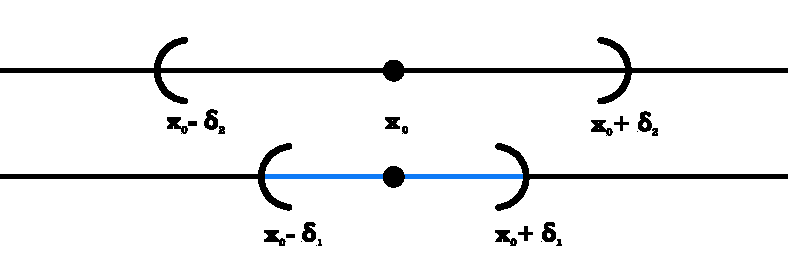
\includegraphics[width=12cm]{./images/interval2.pdf}
\end{figure}

\noindent\textbf{NB!} In generale, se interseco un numero \textbf{finito} di intorni di un certo numero reale $x_0$, ottengo ancora una volta un intorno di quel numero. Lo stesso avviene se interseco più intorni di $+\infty$ (o $-\infty$). Questo discorso però potrebbe non valere quando interseco infiniti intorni.\\

\noindent\textbf{ES.} Prendiamo $x_0 = 0$ e $A_n = D\left(0, \dfrac{1}{n}\right)$ con $n \in \mathbb{N}, n \geq 1$. Il nostro obiettivo è dimostrare che

\begin{equation*}
    B = \underset{\underset{\scriptstyle n \geq 1}{n \in \mathbb{N}}}{\cap} A_n = \{0\}
\end{equation*}

\noindent ovvero che l'intersezione dei vari intorni $A_n$ al variare di $n$ con $n \in \mathbb{N}, n \geq 1$ faccia esattamente $0$. Dividiamo la dimostrazione in due step: innanzitutto, proviamo che $A_n \supseteq \{0\}$ e successivamente che $A_n \subseteq \{0\}$ (in questo modo poi è possibile dire che $A_n = \{0\}$).\\
Partiamo dalla "$\supseteq$", ovvero mostriamo che $0 \in B$. Secondo la definizione di $B$ data precedentemente, ciò risulta equivalente a mostrare che $0$ appartiene a tutti gli insiemi $A_n$. In simboli: $0 \in A_n \quad \forall n \in \mathbb{N}, n \geq 1$. Dato che tutti gli $A_n$ sono centrati in $0$ (perché $A_n = D(0, \frac{1}{n})$), allora:

\begin{equation*}
     0 \in \underset{\underset{\scriptstyle n \geq 1}{n \in \mathbb{N}}}{\cap} A_n \implies \{0\} \subseteq \underset{\underset{\scriptstyle n \geq 1}{n \in \mathbb{N}}}{\cap} A_n
\end{equation*}

\noindent Procediamo ora con la seconda parte della dimostrazione ("$\subseteq$"). Sia $x > 0$ e per contraddizione diciamo che $x \in B$. Ciò significa però anche che $x \in A_n \quad \forall n \in \mathbb{N}, n \geq 1$. Ipotizziamo ora che:

\begin{equation}
    0 < x < \frac{1}{n} \qquad \forall n \in \mathbb{N}, n \geq 1
    \label{eq:11}
\end{equation}

\noindent Dato che l'insieme $\left\{\dfrac{1}{n} : n \geq 1\right\}$ è inferiormente limitato e, in particolare, $inf\left\{\dfrac{1}{n} : n \geq 1\right\} = 0$, ovvero $0$ è il massimo dei minoranti (abbiamo determinato tale valore utilizzando la proprietà di Archimede. Infatti $\forall \varepsilon > 0, \exists \Bar{n} \in \mathbb{N} \ | \ \Bar{n} > \frac{1}{\varepsilon} \implies \frac{1}{\Bar{n}} < \varepsilon$), in (\ref{eq:11}) se $x$ fosse minorante, allora $x \leq max(minoranti) \ (= 0)$, ovvero che $x \leq 0$. Arriviamo quindi ad una contraddizione. Ciò significa che nessun $x > 0$ può appartenere a $B$. \\
Allo stesso modo, sia $x < 0$ per contraddizione:

\begin{equation*}
    -\frac{1}{n} < x < 0 \qquad \forall n \in \mathbb{N}, n \geq 1
\end{equation*}

\noindent Definiamo ora $C = \left\{-\dfrac{1}{n} : n \in \mathbb{N}, n \geq 1\right\}$. Secondo questa definizione di $C$, $x$ rappresenta un maggiorante di questo insieme, ma per la proprietà di Archimede $sup(C) = 0$ (potevamo anche ricavarlo molto più semplicemente ricordandoci che $inf(-A) = -sup(A)$), dove $sup(C)$ è proprio il minimo dei maggioranti di $C$. Arriviamo però ancora una volta ad una contraddizione perché stiamo dicendo che esiste un maggiorante $x < 0$, che è più piccolo del minimo dei maggioranti ($0$). Per questo motivo, $x \geq 0$, quindi nessun $x < 0$ è appartenente a $B$.\\
Dato che come primo step abbiamo dimostrato l'appartenenza di $0$ a $B$ e dato che in questo secondo step abbiamo dimostrato che $B$ non contiene né $x < 0$, né $x > 0$, arriviamo alla conclusione che $B = \{0\}$. Riassumendo quindi presi infiniti intorni e intersecati tra di essi, otteniamo solo il loro centro (che ovviamente non è un intorno).\\

\noindent\textbf{ES.} Un altro esempio di intersezione con un numero infinito di intorni che non restituisce un ulteriore intorno può essere la seguente: 

\begin{equation*}
    \underset{n \geq 1}{\cap} (n, + \infty) = \varnothing
\end{equation*}

\noindent Infatti, se prendiamo un qualsiasi intorno del tipo $(x, +\infty)$ con $x \in \mathbb{R}$ e $x > 0$, esisterà sempre un intorno del tipo $(M, +\infty)$ con $M \in \mathbb{N}$ e $M >> 0, M > x$ (per la proprietà di Archimede) tale che la loro intersezione dia un insieme vuoto.

\subsection{Teorema di unicità del limite}
Sia $f: A \subset \mathbb{R} \xrightarrow{} \mathbb{R}$ e $x_0 \in \widetilde{\mathbb{R}}$ con $x_0$ punto di accumulazione per $A$.\\
Suppongo che:

\begin{equation}
    \lim_{x\to x_0}f(x) = l_1 \in \widetilde{\mathbb{R}}
    \label{eq:12}
\end{equation}

\begin{equation}
    \lim_{x\to x_0}f(x) = l_2 \in \widetilde{\mathbb{R}}
    \label{eq:13}
\end{equation}

\noindent allora $l_1 = l_2$.

\subsubsection{Dimostrazione del teorema di unicità del limite}
Innanzitutto definiamo il primo limite (\ref{eq:12}). $\forall V_{l_1}$ intorno di $l_1$, $\exists U_{x_0}$ intorno di $x_0$ tale che $f(x) \in V_{l_1}$ per ogni $x \in (U_{x_0} \cap A) - \{x_0\}$.\\
Definiamo ora il secondo limite (\ref{eq:13}). $\forall V_{l_2}$ intorno di $l_2$, $\exists U'_{x_0}$ intorno di $x_0$ tale che $f(x) \in V_{l_2}$ per ogni $x \in (U'_{x_0} \cap A) - \{x_0\}$.\\

\noindent\textbf{NB!} Se $x_0 \in \{+\infty, -\infty\}$, non bisogna scrivere il $- \{x_0\}$ durante l'intersezione tra i due insiemi.\\

\noindent Supponiamo ora che $l_1 \neq l_2$. Allora $\exists V_{l_1}, V_{l_2}$ intorni di $l_1$ e $l_2$ rispettivamente tali che $V_{l_1} \cap V_{l_2} = \varnothing$.\\
Supponiamo ora che $l_1, l_2 \in \mathbb{R}$ e che $l_1 < l_2$. Possiamo quindi definire la distanza tra $l_2$ e $l_1$ come $d = l_2 - l_1 > 0$. Se prendiamo ora:

\begin{equation*}
    V_{l_1} = D\left(l_1, \frac{d}{2}\right) \qquad V_{l_2} = D\left(l_2, \frac{d}{2}\right)
\end{equation*}

\noindent abbiamo effettivamente che $V_{l_1} \cap V_{l_2} = \varnothing$. Graficamente:

\begin{figure}[!h]
    \centering
    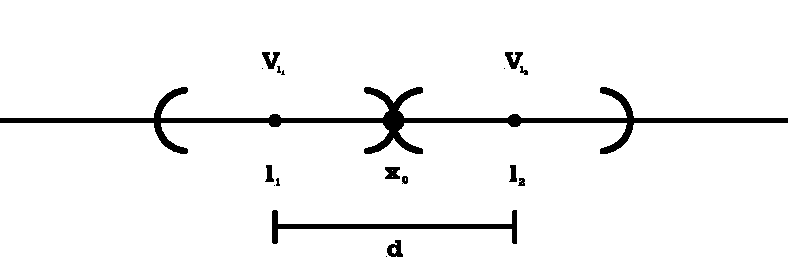
\includegraphics[width=12cm]{./images/interval3.pdf}
\end{figure}

\noindent Chiamiamo ora $W_{x_0} = U_{x_0} \cap U'_{x_0}$, che è un intorno di $x_0$. Sia $x \in (W_{x_0} \cap A) - \{x_0\} \neq \varnothing$ (perché $x_0$ è punto di accumulazione). Allora per la definizione di limite: $f(x) \in V_{l_1}$ (dato che $x \in W_{x_0} \subseteq U_{x_0}$ e se $x \in U_{x_0} \implies f(x) \in V_{l_1}$) e $f(x) \in V_{l_2}$ (dato che $x \in W_{x_0} \subseteq U'_{x_0}$ e se $x \in U'_{x_0} \implies f(x) \in V_{l_2}$). Quindi $f(x) \in V_{l_1} \cap V_{l_2}$, ma prima abbiamo preso apposta $V_{l_1}$ e $V_{l_2}$ tali che $V_{l_1} \cap V_{l_2} = \varnothing$. Siamo quindi arrivati ad una contraddizione. Ne deriva che $l_1 = l_2$ (nella pratica, infatti, non è possibile che una funzione sia arbitrariamente vicina sia ad un $l_1$ che ad un $l_2$ con $l_1 \neq l_2$. Allo stesso modo, se $l_1 = + \infty$ e $l_2 \in \mathbb{R}$, come fa $f(x)$ ad essere arbitrariamente vicina sia a $l_1$, che a $l_2$?!).\\

\noindent Supponiamo ora invece che $l_1 = +\infty$ e che $l_2 \in \mathbb{R}$. Allora abbiamo che $V_{l_1} = (K, + \infty), U_{x_0} = (x_0 - \delta_K, x_0 + \delta_K)$ e $V_{l_2} = (l - \varepsilon, l + \varepsilon), U'_{x_0} = (x_0 - \delta_\varepsilon, x_0 + \delta_\varepsilon)$. Per la definizione di limite quindi abbiamo rispettivamente che: 

\begin{equation*}
    \forall K > 0, \exists \delta_K > 0 : f(x) > K \qquad \forall x \in ((x_0 - \delta_K, x_0 + \delta_K) \cap A) - \{x_0\}
\end{equation*}
\begin{equation*}
    \forall \varepsilon > 0, \exists \delta_\varepsilon > 0 : |f(x) - l_2| < \varepsilon \qquad \forall x \in ((x_0 - \delta_\varepsilon, x_0 + \delta_\varepsilon) \cap A) - \{x_0\}
\end{equation*}

\noindent Ora sia $K > l_2$, allora $d = K - l_2 > 0$ e quindi: $V_{l_1} = (K, + \infty)$ e $V_{l_2} = D\left(l_2, \dfrac{d}{2}\right)$ (dove $\varepsilon = \frac{d}{2}$. Andrebbe bene qualsiasi valore positivo $\varepsilon$ tale che sia inferiore di $d$). In questo modo abbiamo che: $V_{l_1} \cap V_{l_2} = \varnothing$.\\
Sia ora $W_{x_0} = U_{x_0} \cap U'_{x_0}$ e sia $x \in (W_{x_0} \cap A) - \{x_0\} \neq \varnothing$, allora, per gli stessi motivi visti nella precedente dimostrazione, $f(x) \in V_{l_1} \cap V_{l_2}$, ma abbiamo impostato tali intorni per far in modo che $V_{l_1} \cap V_{l_2} = \varnothing$. Ciò significa che non possono coesistere due limiti distinti di $x_0$ con $l_1 = + \infty$ e $l_2 \in \mathbb{R}$.\\

\noindent Supponiamo ora invece che $l_1 = -\infty$ e che $l_2 \in \mathbb{R}$. Allora abbiamo che $V_{l_1} = (- \infty, K), U_{x_0} = (x_0 - \delta_K, x_0 + \delta_K)$ e $V_{l_2} = (l - \varepsilon, l + \varepsilon), U'_{x_0} = (x_0 - \delta_\varepsilon, x_0 + \delta_\varepsilon)$. Per la definizione di limite quindi abbiamo rispettivamente che: 

\begin{equation*}
    \forall K > 0, \exists \delta_K > 0 : f(x) < K \qquad \forall x \in ((x_0 - \delta_K, x_0 + \delta_K) \cap A) - \{x_0\}
\end{equation*}
\begin{equation*}
    \forall \varepsilon > 0, \exists \delta_\varepsilon > 0 : |f(x) - l_2| < \varepsilon \qquad \forall x \in ((x_0 - \delta_\varepsilon, x_0 + \delta_\varepsilon) \cap A) - \{x_0\}
\end{equation*}

\noindent Ora sia $K < l_2$, allora $d = l_2 - K > 0$ e quindi: $V_{l_1} = (-\infty, K)$ e $V_{l_2} = D\left(l_2, \dfrac{d}{2}\right)$ (dove $\varepsilon = \frac{d}{2}$. Andrebbe bene qualsiasi valore positivo $\varepsilon$ tale che sia inferiore di $d$). In questo modo abbiamo che: $V_{l_1} \cap V_{l_2} = \varnothing$.\\
Sia ora $W_{x_0} = U_{x_0} \cap U'_{x_0}$ e sia $x \in (W_{x_0} \cap A) - \{x_0\} \neq \varnothing$, allora, per gli stessi motivi visti nella precedente dimostrazione, $f(x) \in V_{l_1} \cap V_{l_2}$, ma abbiamo impostato tali intorni per far in modo che $V_{l_1} \cap V_{l_2} = \varnothing$. Ciò significa che non possono coesistere due limiti distinti di $x_0$ con $l_1 = - \infty$ e $l_2 \in \mathbb{R}$.\\

\noindent Infine, supponiamo ora invece che $l_1 = -\infty$ e che $l_2 = +\infty$. Allora abbiamo che $V_{l_1} = (- \infty, K), U_{x_0} = (x_0 - \delta_K, x_0 + \delta_K)$ e $V_{l_2} = (M, +\infty), U'_{x_0} = (x_0 - \delta_M, x_0 + \delta_M)$. Per la definizione di limite quindi abbiamo rispettivamente che: 

\begin{equation*}
    \forall K > 0, \exists \delta_K > 0 : f(x) < K \qquad \forall x \in ((x_0 - \delta_K, x_0 + \delta_K) \cap A) - \{x_0\}
\end{equation*}
\begin{equation*}
    \forall M > 0, \exists \delta_M > 0 : f(x) > M \qquad \forall x \in ((x_0 - \delta_M, x_0 + \delta_M) \cap A) - \{x_0\}
\end{equation*}

\noindent Ora sia $K < M$ e quindi: $V_{l_1} = (-\infty, K)$ e $V_{l_2} = (M, +\infty)$. In questo modo abbiamo che: $V_{l_1} \cap V_{l_2} = \varnothing$.\\
Sia ora $W_{x_0} = U_{x_0} \cap U'_{x_0}$ e sia $x \in (W_{x_0} \cap A) - \{x_0\} \neq \varnothing$, allora, per gli stessi motivi visti nella precedente dimostrazione, $f(x) \in V_{l_1} \cap V_{l_2}$, ma abbiamo impostato tali intorni per far in modo che $V_{l_1} \cap V_{l_2} = \varnothing$. Ciò significa che non possono coesistere due limiti distinti di $x_0$ con $l_1 = - \infty$ e $l_2 = +\infty$.\\

\subsection{Teorema di permanenza del segno}
Sia $f: A \subset \mathbb{R} \xrightarrow{} \mathbb{R}$ e $x_0 \in \widetilde{\mathbb{R}}$ punto di accumulazione per $A$. Se:

\begin{equation*}
    \lim_{x \to x_0} f(x) = l \in (0, + \infty) \cup \{+\infty\} \qquad [oppure \ 
 l \in (- \infty, 0) \cup \{-\infty\}]
\end{equation*}

\noindent allora $\exists K > 0, \exists U_{x_0} \ intorno \ di \ x_0 \ | \ f(x) > K \ (> 0) \quad \forall x \in (U_{x_0} \cap A) - \{x_0\}$ (oppure $f(x) < -K \ (< 0)$, se $l$ appartiene al secondo intorno definito tra le parentesi quadre).\\

\noindent\textbf{Link:} \href{https://www.geogebra.org/m/qbgp526U}{Teorema di permanenza del segno}.

\subsubsection{Dimostrazione del teorema della permanenza del segno per $l = +\infty$}
Dato che $\forall K \in \mathbb{R}, \exists U_{x_0} \ intorno \ di \ x_0 \ | \ f(x) > K \qquad \forall x \in (U_{x_0} \cap A) - \{x_0\}$, allora se fissiamo $\Bar{K} > 0$ e lo applichiamo a questa definizione, otteniamo che $f(x) > \Bar{K} \qquad \forall x \in (U_{x_0} \cap A) - \{x_0\}$.

\subsubsection{Dimostrazione del teorema della permanenza del segno per $l \in \mathbb{R}, l > 0$}
Se $l \in \mathbb{R}, l > 0$, allora $V_l = (l - \varepsilon, l + \varepsilon)$ e quindi: $\forall \varepsilon > 0, \exists U_{x_0} \ intorno \ di \ x_0 : |f(x) - l| < \varepsilon \qquad \forall x \in (U_{x_0} \cap A) - \{x_0\}$. Ma dire che $|f(x) - l| < \varepsilon$, significa dire che $l - \varepsilon < f(x) < l + \varepsilon$.\\
Determiniamo ora una $\varepsilon > 0$ tale per cui $0 < l - \varepsilon$ (così anche $f(x) > 0$). Poniamo quindi $\varepsilon = \frac{l}{2}$ (bastava scegliere una $\varepsilon \ | \ l - \varepsilon > 0$), si ottiene così: 

\begin{equation*}
    0 < \frac{l}{2} < f(x) < \frac{3}{2}l \qquad \forall x \in (U_{x_0} \cap A) - \{x_0\}
\end{equation*}

\noindent dove $K = \frac{l}{2}$.

\subsubsection{Dimostrazione del teorema della permanenza del segno per $l \in \mathbb{R}, l < 0$}
Se $l \in \mathbb{R}, l < 0$, allora $V_l = (l - \varepsilon, l + \varepsilon)$ e quindi $\forall \varepsilon > 0, \exists U_{x_0} \ intorno \ di \ x_0 : |f(x) - l| < \varepsilon \qquad \forall x \in (U_{x_0} \cap A) - \{x_0\}$. Ma dire che $|f(x) - l| < \varepsilon$, significa dire che $l - \varepsilon < f(x) < l + \varepsilon$.\\
Determiniamo ora una $\varepsilon > 0$ tale per cui $l + \varepsilon < 0$ (così anche $f(x) < 0$). Poniamo quindi $\varepsilon = -\frac{l}{2}$ (bastava scegliere una $\varepsilon \ | \ l + \varepsilon < 0$; $\varepsilon > 0$, perché $l < 0$), si ottiene così:

\begin{equation*}
    \frac{3}{2}l < f(x) < \frac{l}{2} \qquad \forall x \in (U_{x_0} \cap A) - \{x_0\}
\end{equation*}

\noindent dove $\frac{3}{2} l < \frac{l}{2}$ perché $l < 0$ e dove $K = \frac{l}{2}$.

\subsubsection{Dimostrazione del teorema della permanenza del segno per $l = - \infty$}
Dato che $\forall K \in \mathbb{R}, \exists U_{x_0} \ intorno \ di \ x_0 \ | \ f(x) < -K \qquad \forall x \in (U_{x_0} \cap A) - \{x_0\}$, allora se fissiamo $\Bar{K} < 0$ e lo applichiamo a questa definizione, otteniamo che $f(x) < \Bar{K} \qquad \forall x \in (U_{x_0} \cap A) - \{x_0\}$.

\subsection{Teorema di limitatezza locale}
Sia $f: A \subset \mathbb{R} \xrightarrow{} \mathbb{R}$ e $x_0 \in \widetilde{\mathbb{R}}$ un punto di accumulazione per $A$.\\
Sia $\lim_{x \to x_0} f(x) = l \in \mathbb{R}$. Allora $\exists U_{x_0}$ intorno di $x_0$ tale che $\{f(x) : x \in U_{x_0} \cap A\}$ è limitato.

\subsubsection{Dimostrazione del teorema di limitatezza locale}
Dato che $\varepsilon > 0, \exists U_{x_0}$ intorno di $x_0$ tale che $l - 1 < f(x) < l + 1 \qquad \forall x \in (U_{x_0} \cap A) - \{x_0\}$.\\
Ora se $x_0 \notin A \implies (U_{x_0} \cap A) = (U_{x_0} \cap A) - \{x_0\}$. Mentre se $x_0 \in A$, chiamo $a = min\{f(x_0), l - 1\}$ e chiamo $b = max\{f(x_0), l + 1\}$. Allora si ha che $a \leq f(x) \leq b \qquad \forall x \in (U_{x_0} \cap A)$.

\subsection{Teorema del confronto (I)}
Siano $f, g: A \subset \mathbb{R} \xrightarrow{} \mathbb{R}$ e sia $x_0 \in \widetilde{\mathbb{R}}$ punto di accumulazione per $A$. Allora:

\begin{enumerate}[label=\alph{enumi})]
    \item se $\lim_{x \to x_0} f(x) = l_1 \in \mathbb{R}$ e se $\lim_{x \to x_0} g(x) = l_2 \in \mathbb{R}$, con $l_1 < l_2$, si ha che: $$\exists U_{x_0} \ intorno \ di \ x_0 \ | \ f(x) < g(x) \qquad \forall x \in (U_{x_0} \cap A) - \{x_0\}$$
    \item se $\lim_{x \to x_0} f(x) = -\infty$ e se $\lim_{x \to x_0} g(x) = l \in \mathbb{R} \cup \{+\infty\}$, si ha che: $$\exists U_{x_0} \ intorno \ di \ x_0 \ | \ f(x) < g(x) \qquad \forall x \in (U_{x_0} \cap A) - \{x_0\}$$
    \item se $\lim_{x \to x_0} f(x) = l \in \mathbb{R}$ e se $\lim_{x \to x_0} g(x) = +\infty$, si ha che: $$\exists U_{x_0} \ intorno \ di \ x_0 \ | \ f(x) < g(x) \qquad \forall x \in (U_{x_0} \cap A) - \{x_0\}$$
\end{enumerate}

\subsubsection{Dimostrazione del punto a) del teorema del confronto (I)}
Siano $l_1 < l_2$ con $l_1, l_2 \in \mathbb{R}$. \\
Se $\lim_{x \to x_0} f(x) = l_1$, fissato $\varepsilon > 0, \exists U'_{x_0}$ intorno di $x_0$ tale che $l_1 - \varepsilon < f(x) < l_1 + \varepsilon \qquad \forall x \in (U'_{x_0} \cap A) - \{x_0\}$.\\
Se $\lim_{x \to x_0} g(x) = l_2$, fissato $\varepsilon > 0, \exists U''_{x_0}$ intorno di $x_0$ tale che $l_2 - \varepsilon < g(x) < l_2 + \varepsilon \qquad \forall x \in (U''_{x_0} \cap A) - \{x_0\}$.\\
Se $x \in (U'_{x_0} \cap U''_{x_0} \cap A) - \{x_0\}$, scelgo $\varepsilon > 0$ tale che: 

\begin{equation*}
    (f(x) < ) \ l_1 + \varepsilon \leq l_2 - \varepsilon \ (< g(x))
\end{equation*}

\noindent Scegliamo quindi $\varepsilon = \frac{l_2 - l_1}{2} > 0$ (ovvero metà della distanza tra $l_2$ e $l_1$). Per $x \in (U'_{x_0} \cap U''_{x_0} \cap A) - \{x_0\}$ si ha che:

\begin{equation*}
    f(x) < l_1 + \varepsilon = l_1 + \frac{l_2 - l_1}{2} = \frac{l_2 + l_1}{2}
\end{equation*}

\begin{equation*}
    g(x) > l_2 - \varepsilon = l_2 - \frac{l_2 - l_1}{2} = \frac{l_2 + l_1}{2}
\end{equation*}

\begin{equation*}
    \implies f(x) < \frac{l_2 + l_1}{2} < g(x) \qquad \forall x \in (U'_{x_0} \cap U''_{x_0} \cap A) - \{x_0\}
\end{equation*}

\subsubsection{Dimostrazione del punto b) del teorema del confronto (I)}
Se $\lim_{x \to x_0} f(x) = - \infty$, significa che $\forall K \in \mathbb{R}, \exists U'_{x_0}$ intorno di $x_0$ tale che $f(x) < K \qquad \forall x \in (U'_{x_0} \cap A) - \{x_0\}$; mentre se $\lim_{x \to x_0} g(x) = l \in \mathbb{R}$, allora fissato $\varepsilon > 0, \exists U''_{x_0}$ intorno di $x_0$ tale che $l - \varepsilon < g(x) < l + \varepsilon \qquad \forall x \in (U''_{x_0} \cap A) - \{x_0\}$.\\
Ora se $x \in (U'_{x_0} \cap U''_{x_0} \cap A) - \{x_0\}$ e imponiamo che $K < l$, significa che:

\begin{equation*}
    (f(x) <) \ K \leq l - \varepsilon \ (< g(x))
\end{equation*}

\noindent quindi se $\varepsilon \leq |l - K|$, si ha che al più $K = l - \varepsilon$, ovvero che:

\begin{equation*}
    g(x) > l - \varepsilon = l - l + K = K \implies f(x) < K < g(x) \implies f(x) < g(x)
\end{equation*}

\subsubsection{Dimostrazione del punto c) del teorema del confronto (I)}
Se $\lim_{x \to x_0} f(x) = l \in \mathbb{R}$, significa che $\forall \varepsilon > 0, \exists U'_{x_0}$ intorno di $x_0$ tale che $|f(x) - l| < \varepsilon \qquad \forall x \in (U'_{x_0} \cap A) - \{x_0\}$; mentre se $\lim_{x \to x_0} g(x) = +\infty$, allora fissato $\forall K \in \mathbb{R}, \exists U''_{x_0}$ intorno di $x_0$ tale che $g(x) > K \qquad \forall x \in (U''_{x_0} \cap A) - \{x_0\}$.\\
Ora se $x \in (U'_{x_0} \cap U''_{x_0} \cap A) - \{x_0\}$ e imponiamo che $K > l$, significa che:

\begin{equation*}
    (f(x) <)\ l + \varepsilon \leq K \ (< g(x))
\end{equation*}

\noindent quindi se $\varepsilon \leq |K - l|$, si ha che al più $K = l + \varepsilon$, ovvero che:

\begin{equation*}
    g(x) > K = l + \varepsilon \implies f(x) < l + \varepsilon < g(x) \implies f(x) < g(x)
\end{equation*}

\begin{wrapfigure}{r}{0.21\textwidth}
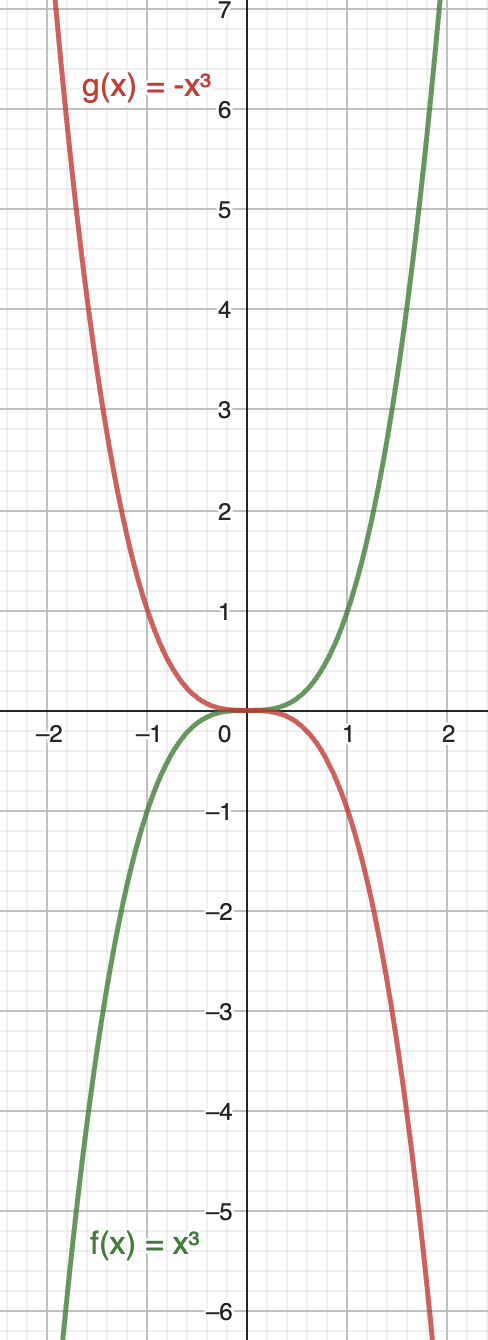
\includegraphics[width=0.9\linewidth]{images/comparisonTheoremI.png} 
\end{wrapfigure}

\noindent\textbf{Osservazione nel punto a):} \\
\noindent Cosa accadrebbe se $l_1 \leq l_2$? In altre parole, posso dire che $f(x) \leq g(x) \ \forall x \in (U'_{x_0} \cap U''_{x_0} \cap A) - \{x_0\}$? \\
No, infatti se $x_0 = 0$ e $f(x) = x^3$ e $g(x) = -x^3 \ \forall x \in (U'_{x_0} \cap U''_{x_0} \cap A) - \{x_0\}$ con $A = D_f = \mathbb{R}$, si ha che:

\begin{equation*}
    \lim_{x \to 0} f(x) = 0 = \lim_{x \to 0} g(x) \quad (ovvero \ l_1 = l_2 = 0)
\end{equation*}

\noindent ovvero in ogni intorno di $0$, $U_0 = D(0, \delta), \forall \delta > 0$, si ha che:

\begin{itemize}
    \item per $x > 0$:
    \begin{itemize}
        \item $f(x) > 0$;
        \item $g(x) < 0$;
    \end{itemize}
    \item per $x < 0$:
    \begin{itemize}
        \item $f(x) < 0$;
        \item $g(x) > 0$;
    \end{itemize}
\end{itemize}

\noindent In altre parole, non abbiamo un intorno del punto $0$, in cui si mantiene una relazione di segno costante.

\subsection{Teorema del confronto II}
Siano $f, g: A \subset \mathbb{R} \xrightarrow{} \mathbb{R}$ con $A \neq \varnothing$ e $x_0 \in \widetilde{\mathbb{R}}$ punto di accumulazione per $A$. Allora:

\begin{enumerate}[label=\alph{enumi})]
    \item se $\lim_{x \to x_0} f(x) = l_1 \in \mathbb{R}$ e se $\lim_{x \to x_0} g(x) = l_2 \in \mathbb{R}$ e se $\exists U_{x_0} \ intorno \ di \ x_0 \ | \ f(x) \leq g(x) \qquad \forall x \in (U_{x_0} \cap A) - \{x_0\}$, allora $l_1 \leq l_2$.
    \item se $\lim_{x \to x_0} g(x) = -\infty$ e se $\exists U_{x_0} \ intorno \ di \ x_0 \ | \ f(x) \leq g(x) \qquad \forall x \in (U_{x_0} \cap A) - \{x_0\}$, allora $\exists \lim_{x \to x_0} f(x) = - \infty$.
     \item se $\lim_{x \to x_0} f(x) = +\infty$ e se $\exists U_{x_0} \ intorno \ di \ x_0 \ | \ f(x) \leq g(x) \qquad \forall x \in (U_{x_0} \cap A) - \{x_0\}$, allora $\exists \lim_{x \to x_0} g(x) = + \infty$.
\end{enumerate}

\begin{wrapfigure}{r}{0.5\textwidth}
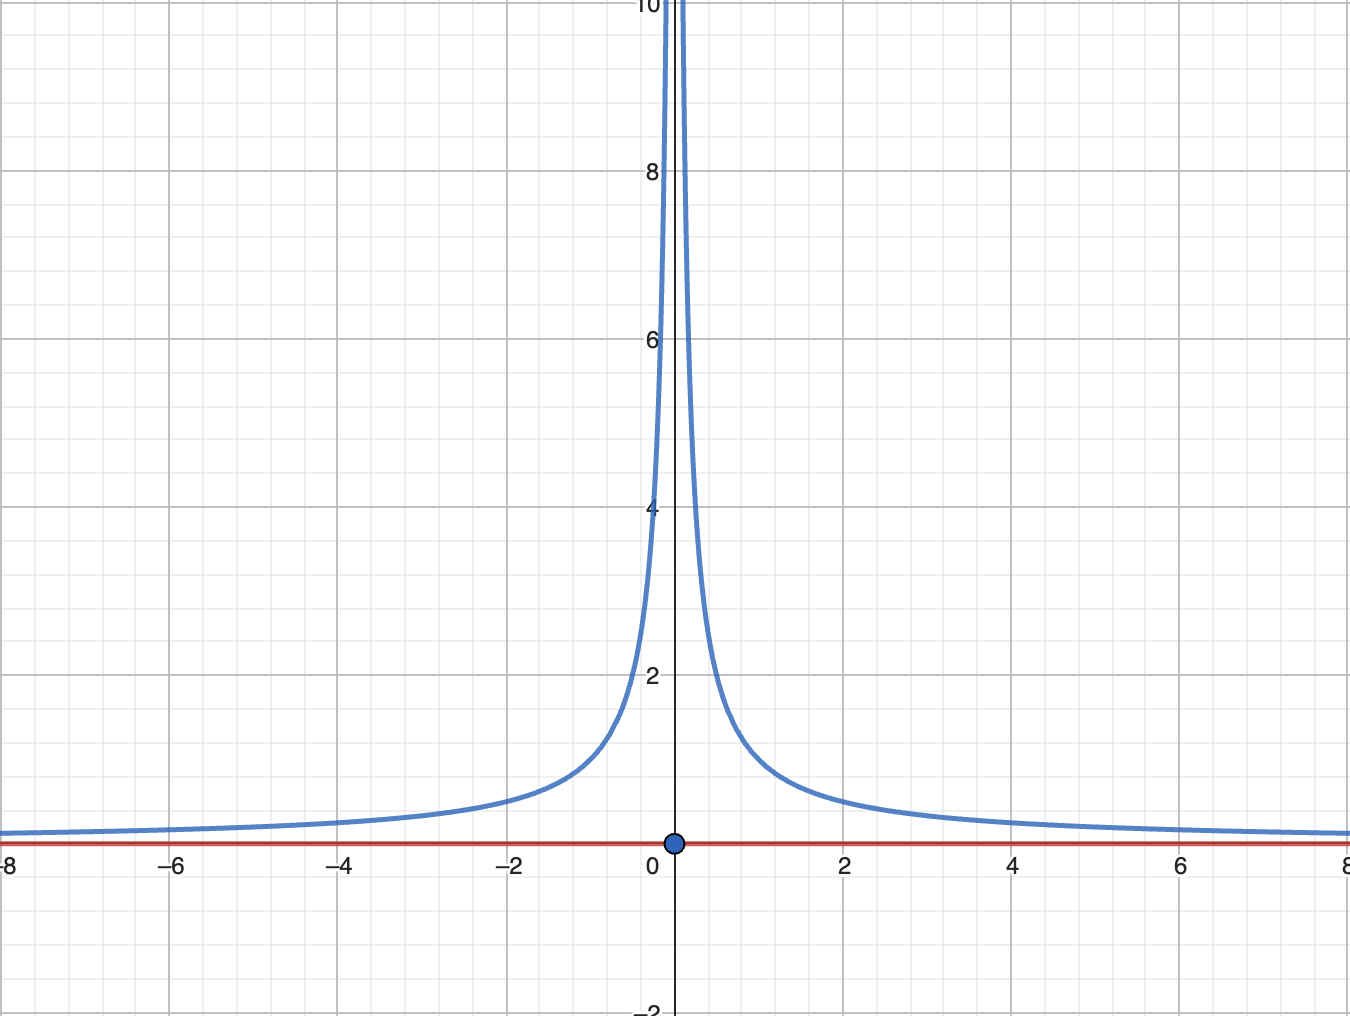
\includegraphics[width=0.9\linewidth]{images/comparisonTheoremII-1.png} 
\end{wrapfigure}

\noindent\textbf{Osservazione:} \\
\noindent Cosa accadrebbe se $f(x) < g(x)$? In altre parole, posso concludere che $l_1 < l_2$?\\
No, perché preso $f(x) = 0 \ \forall x \in \mathbb{R}$ e 

\begin{wrapfigure}{l}{0.47\textwidth}
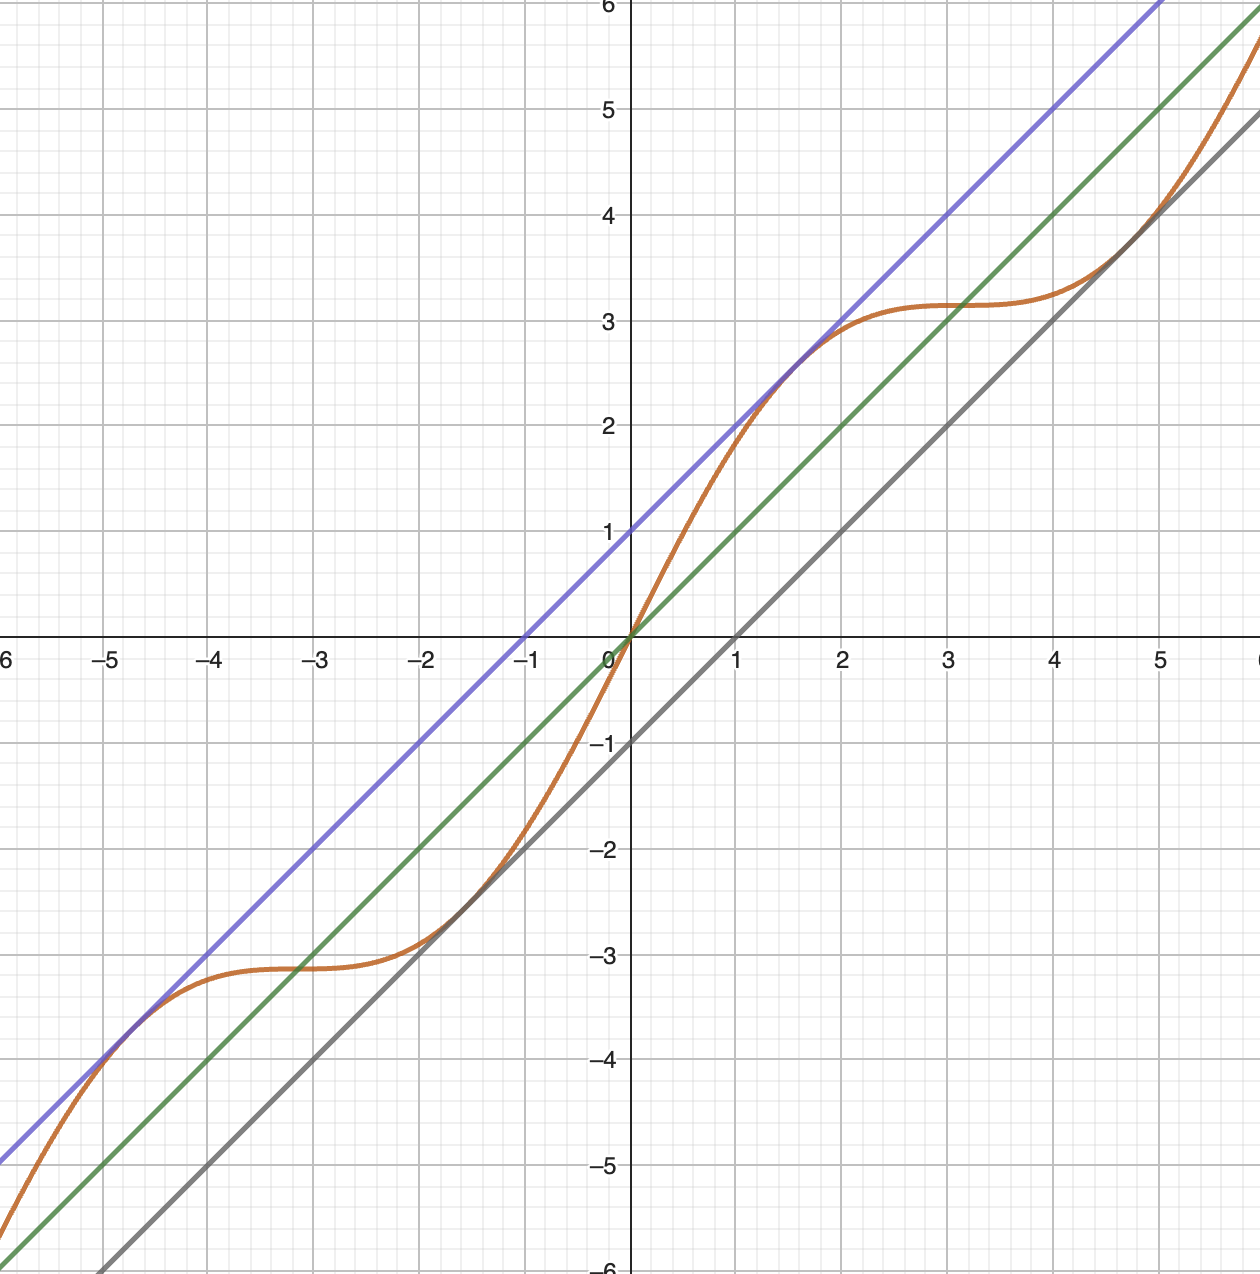
\includegraphics[width=0.9\linewidth]{images/comparisonTheoremII-2.png} 
\end{wrapfigure}

\begin{equation*}
    g(x) = 
    \begin{cases}
        \frac{1}{x} \ se \ x > 0 \\
        0 \ se \ x = 0 \\
        -\frac{1}{x} \ se \ x < 0
    \end{cases}
\end{equation*}

\noindent si ha che $\forall x \in (U_0 \cap \mathbb{R}) - \{0\}, f(x) < g(x)$. Lo stesso vale per $x \in U_{+\infty} \cap \mathbb{R}$. Infatti:

\begin{equation*}
    \lim_{x \to +\infty} g(x) = 0 = \lim_{x \to +\infty} f(x) \quad (ovvero \ l_1 = l_2)
\end{equation*}

\noindent Questo significa che non possiamo concludere che $f(x) < g(x)$, ma $f(x) \leq g(x)$.\\

\noindent\textbf{ES.} Mostriamo che il teorema funziona anche quando una delle due funzioni non ammette limite.\\
Diciamo che:

\begin{equation*}
    \lim_{x \to + \infty} g(x) = \lim_{x \to + \infty} x + \sin(x) = + \infty
\end{equation*}

\noindent Dato che $\sin(x) \geq - 1, \forall x \in \mathbb{R}$, allora:

\begin{equation*}
    g(x) = x + \sin(x) \geq x - 1 = f(x) \qquad \forall x \in \mathbb{R}
\end{equation*}

\noindent Dato che $\lim_{x \to + \infty} f(x) = \lim_{x \to + \infty} x - 1 = + \infty$, allora $\exists \lim_{x \to + \infty} x + \sin(x) = + \infty$.\\

\noindent\textbf{ES.} Mostriamo che il teorema funziona anche quando una delle due funzioni non ammette limite.\\
Diciamo che:

\begin{equation*}
    \lim_{x \to - \infty} g(x) = \lim_{x \to - \infty} x + \sin(x) = - \infty
\end{equation*}

\noindent Dato che $\sin(x) \leq 1, \forall x \in \mathbb{R}$, allora:

\begin{equation*}
    g(x) = x + \sin(x) \leq x + 1 = f(x) \qquad \forall x \in \mathbb{R}
\end{equation*}

\noindent Dato che $\lim_{x \to - \infty} f(x) = \lim_{x \to - \infty} x + 1 = - \infty$, allora $\exists \lim_{x \to - \infty} x + \sin(x) = - \infty$.\\

\subsection{Teorema delle tre funzioni o dei due carabinieri}
Siano $f, g, h: A \subset \mathbb{R} \xrightarrow{} \mathbb{R}$, con $A \neq \varnothing$ e $x_0 \in \widetilde{\mathbb{R}}$ punto di accumulazione per $A$. Inoltre, $\exists \lim_{x \to x_0} f(x) = l \in \mathbb{R}$, $\exists \lim_{x \to x_0} g(x) = l \in \mathbb{R}$ (ovvero $f(x)$ e $g(x)$, per $x$ che tende a $x_0$, tendono allo stesso valore reale $l$) e $\exists U_{x_0} \ intorno \ di \ x_0 \ | \ f(x) \leq h(x) \leq g(x) \qquad \forall x \in (U_{x_0} \cap A) - \{x_0\}$. Allora possiamo affermare con certezza che:

\begin{equation*}
    \exists \lim_{x \to x_0} h(x) = l
\end{equation*}

\noindent\textbf{NB!} Questo teorema vale solo per limiti reali.

\subsubsection{Dimostrazione del teorema delle tre funzioni o dei due carabinieri}
Sia $\varepsilon > 0$, allora $\exists U'_{x_0}, U''_{x_0}$ intorni di $x_0$ tali che:
\begin{gather*}
    |f(x) - l| < \varepsilon \qquad \forall x \in (U'_{x_0} \cap A) - \{x_0\}\\
    |g(x) - l| < \varepsilon \qquad \forall x \in (U''_{x_0} \cap A) - \{x_0\}
\end{gather*}

\noindent Sia $W_{x_0} = U'_{x_0} \cap U''_{x_0} \cap A$ intorno di $x_0$. Se $x \in (W_{x_0} \cap A) - \{x_0\}$, valgono allora tutte le disequazioni scritte precedentemente. Quindi si ha che:

\begin{equation*}
    l - \varepsilon < f(x) \ (< l + \varepsilon) \quad (disequazione \ del \ limite \ di \ f)
\end{equation*}
\begin{equation*}
    f(x) \leq h(x) \leq g(x) \quad (per \ ipotesi)
\end{equation*}
\begin{equation*}
    (l - \varepsilon <) \ g(x) < l + \varepsilon \quad (disequazione \ del \ limite \ di \ g)
\end{equation*}

\noindent Quindi $l - \varepsilon \leq h(x) < l + \varepsilon$, cioè $|h(x) - l| < \varepsilon$. Abbiamo fatto vedere che:
\begin{equation*}
    \forall \varepsilon > 0, \exists W_{x_0} \ intorno \ di \ x_0 : |h(x) - l| < \varepsilon \quad \forall x \in (W_{x_0} \cap A) - \{x_0\} \implies \lim_{x \to x_0} h(x) = l
\end{equation*}

\noindent\textbf{ES.} Utilizziamo il teorema dei due carabinieri per dimostrare che:

\begin{equation*}
    \exists \lim_{x \to 0} h(x) = \lim_{x \to 0} x\sin\left(\frac{1}{x}\right)
\end{equation*}

\noindent Innanzitutto, determiniamo il dominio di $h(x)$: $D_h: \mathbb{R} - \{0\}$ e capiamo che $0$ è punto di accumulazione per $D_h$.\\
A questo punto, consideriamo $|h(x)| \geq 0 \implies |x \sin \frac{1}{x}| \geq 0$. Dato che $|ab| = |a||b|$, allora si ha che $0 \leq |x\sin\frac{1}{x}| = |x||\sin\frac{1}{x}|$.\\
Ora, siccome $0 \leq |\sin x| \leq 1$, allora $0 \leq |x||\sin\frac{1}{x}| \leq |x|$. Quindi se $f(x) = 0$ (una funzione costante nulla) e $g(x) = |x|$, allora si ha che:

\begin{equation*}
    f(x) \leq |h(x)| \leq g(x)
\end{equation*}

\noindent Dato che se $x \to 0$, allora $f(x) \to 0$, così come se $x \to 0$, allora $g(x) \to 0$, allora possiamo concludere che, per il teorema dei due carabinieri, $|h(x)| \to 0$. In altre parole:

\begin{equation*}
    \exists \lim_{x \to 0} \left|x\sin\left(\frac{1}{x}\right)\right| = 0
\end{equation*}

\noindent Prendiamo ora $h(x) = x\sin\frac{1}{x}$, dato che $\sin\frac{1}{x} \leq 1$, allora $x\sin\frac{1}{x} \leq x$. Allo stesso tempo però $\sin\frac{1}{x} \geq -1$ e quindi $\sin\frac{1}{x} \geq -x$. Quindi possiamo scrivere:

\begin{equation*}
    -x \leq x\sin\frac{1}{x} \leq x
\end{equation*}

\noindent Quindi se $\lim_{x \to 0} x = 0$ e $\lim_{x \to 0} -x = 0$, allora $\exists \lim_{x \to 0} |x\sin\frac{1}{x}| = 0$. Non ci resta solo che verificare l'esistenza dei primi due limiti. In entrambi si ha che:

\begin{equation*}
    \forall \varepsilon > 0, \exists \delta_\varepsilon > 0 : |h(x) - 0| < \varepsilon \qquad \forall x \in (\mathbb{R} - \{0\} \cap (-\delta_\varepsilon, \delta_\varepsilon))
\end{equation*}

\noindent ovvero: $|-x| = |x| < \varepsilon \implies (-\varepsilon, \varepsilon)$ e quindi $\delta_\varepsilon = \varepsilon$.\\

\subsection{Funzione di Dirichlet}
Sia:

\begin{equation*}
    f(x) = 
    \begin{cases}
        -1 \qquad \ se \ x \in \mathbb{Q} \\
        1 \qquad \ \ \ se \ x \in \mathbb{R - Q}
    \end{cases}
\end{equation*}

\noindent Innanzitutto, notiamo che $f(0) = -1$, che $|f(x)| = 1 \quad \forall x \in \mathbb{R}$, che $\lim_{x \to x_0} |f(x)| = 1$ e, infine, che $\nexists \lim_{x \to x_0} f(x)$.\\
Supponiamo però che $\lim_{x \to x_0} f(x) = l$. Se $l = -1, \forall \varepsilon > 0$ varrebbe la definizione di limite. Fissiamo allora $\varepsilon = \frac{1}{2}$, allora $\exists U_{x_0} \ intorno \ di \ x_0 : |f(x) - (-1)| < \frac{1}{2} \qquad \forall x \in U_{x_0} - \{x_0\}$. Ma ciò è falso perché $-\frac{3}{2} < f(x) < -\frac{1}{2} \qquad \forall x \in U_{x_0} - \{x_0\}$, ma in ogni intorno bucato di $x_0$, sono presenti infiniti razionali e irrazionali e il valore ottenuto da razionali mappati nella funzione $f(x)$ ($-1$) è diverso da quello ottenuto mappando irrazionali ($1$). Dato quindi che si arriva ad una contraddizione, $l = -1$ non è il valore di $\lim_{x \to x_0} f(x)$.\\
Analogamente, se $l = 1$, allora $|f(x) - 1| < \frac{1}{2} \implies \frac{1}{2} < f(x) < \frac{3}{2} \qquad \forall x \in U_{x_0} - \{x_0\}$ e, anche qui, ciò non vale per tutti quegli infiniti numeri razionali che si sono in un intorno bucato di $x_0$. In altre parole, $l = 1$ non è il valore di $\lim_{x \to x_0} f(x)$.\\
Se invece:

\begin{itemize}
    \item $l > 1$, ma $l - \frac{1}{2} > 1$ (cioè l'estremo inferiore di $V_l$ è più grande di $1$);
    \item $l < -1$, ma $l + \frac{1}{2} < -1$ (cioè l'estremo superiore di $V_l$ è più piccolo di $-1$);
    \item $-1 < l < 1$, ma $l - \frac{1}{2} > - 1$ e $l + \frac{1}{2} < 1$.
\end{itemize}

\noindent allora per il teorema della limitatezza locale, esiste un intorno di $x_0$ tale che $\{f(x) : x \in U_{x_0} \cap A\}$ è limitato. In altre parole, imponendo tali vincoli si costruisce un insieme di valori $f(x) > 1$ o $f(x) < -1$ oppure ancora $-1 < f(x) < 1$. \\

\noindent\textbf{Osservazioni:} Sia $A \neq \varnothing$ e $f: A \subset \mathbb{R} \xrightarrow{} \mathbb{R}$ e $x_0 \in \widetilde{\mathbb{R}}$ di accumulazione per $A$. Allora si ha che:

\begin{enumerate}
    \item $\lim_{x \to x_0} f(x) = l \in \mathbb{R} \iff \lim_{x \to x_0} (f(x) - l) = 0$;
    \item $\lim_{x \to x_0} f(x) = 0 \iff \lim_{x \to x_0} |f(x)| = 0$;
    \item $\lim_{x \to x_0} f(x) = l \in \mathbb{R} - \{0\} \implies \lim_{x \to x_0} |f(x)| = |l|$ (è solo un'implicazione in questo caso. Infatti, se fosse un $\iff$, allora esisterebbero controesempi come la funzione di Dirichlet);
    \item $\lim_{x \to x_0} f(x) = 0 \iff \lim_{x \to x_0} [f(x)]^2 = 0$;
\end{enumerate}

\noindent Di seguito, verifichiamo i vari punti qui sopra elencati. \\

\noindent\textbf{Verifica del punto 1)}\\
\noindent Innanzitutto, scriviamo le due definizioni di limiti:

\begin{equation*}
    \forall \varepsilon > 0, \exists U_{x_0} \ intorno \ di \ x_0 : |f(x) - l| < \varepsilon \qquad \forall x \in (U_{x_0} \cap A) - \{x_0\}
\end{equation*}
\begin{equation*}
    \forall \varepsilon > 0, \exists V_{x_0} \ intorno \ di \ x_0 : |f(x) - l - 0| < \varepsilon \qquad \forall x \in (V_{x_0} \cap A) - \{x_0\}
\end{equation*}

\noindent Possiamo quindi notare come le due espressioni risultino analoghe.\\

\noindent\textbf{Verifica del punto 2)}\\
\begin{equation*}
    \forall \varepsilon > 0, \exists U_{x_0} \ intorno \ di \ x_0 : |f(x) - 0| < \varepsilon \qquad \forall x \in (U_{x_0} \cap A) - \{x_0\}
\end{equation*}
\begin{equation*}
    \forall \varepsilon > 0, \exists V_{x_0} \ intorno \ di \ x_0 : ||f(x)| - 0| - 0| < \varepsilon \qquad \forall x \in (V_{x_0} \cap A) - \{x_0\}
\end{equation*}

\noindent Dato che $||f(x)|| = |f(x)|$, allora $||f(x)| - 0| = |f(x) - 0|$. Possiamo quindi notare ancora una volta l'uguaglianza tra le due espressioni.\\

\noindent\textbf{Verifica del punto 3)}\\
Per la II disuguaglianza triangolare ($||a| - |b|| \leq |a - b|$), si ha che $||f(x)| - |l|| \leq |f(x) - l|$. \\
Per ipotesi invece: 

\begin{equation*}
    \forall \varepsilon > 0, \exists U_{x_0} \ intorno \ di \ x_0 : |f(x) - l| < \varepsilon \qquad \forall x \in (U_{x_0} \cap A) - \{x_0\}
\end{equation*}

\noindent Ora quindi sappiamo che $||f(x)| - |l|| \leq |f(x) - l| < \varepsilon$, allora possiamo dire che:

\begin{equation*}
    \forall \varepsilon > 0, \exists U_{x_0} \ intorno \ di \ x_0 : ||f(x)| - |l|| < \varepsilon \qquad \forall x \in (U_{x_0} \cap A) - \{x_0\}
\end{equation*}

\noindent\textbf{Verifica del punto 4)}\\
\noindent Dimostriamo, innanzitutto, l'implicazione. Quindi:

\begin{equation*}
    \forall \varepsilon > 0, \exists U_{x_0} \ intorno \ di \ x_0 : |f(x) - 0| < \varepsilon \qquad \forall x \in (U_{x_0} \cap A) - \{x_0\}
\end{equation*}

\noindent Notiamo però che se $|f(x)|^2 < \varepsilon^2$, allora anche $[f(x)]^2 < \varepsilon^2$, infatti:

\begin{itemize}
    \item $f(x) \geq 0 \implies |f(x)| = f(x)$;
    \item $f(x) \leq 0 \implies [|f(x)|]^2 = [f(x)]^2$
\end{itemize}

\noindent Se invece consideriamo la controimplicazione:

\begin{equation*}
    \forall \varepsilon > 0, \exists U_{x_0} \ intorno \ di \ x_0 : |[f(x)]^2| < \varepsilon \qquad \forall x \in (U_{x_0} \cap A) - \{x_0\}
\end{equation*}

\noindent Dato che $|[f(x)]^2| < \varepsilon$, allora $|f(x)| < \sqrt{\varepsilon}$ (ovvero $- \sqrt{\varepsilon} < f(x) < \sqrt{\varepsilon}$). Per la proprietà 2) verificata precedentemente, se $lim_{x \to 0} |f(x)| = 0$, allora $\lim_{x \to 0} f(x) = 0$.

\subsection{Teorema del limite della somma}
Siano $f, g: A \subset \mathbb{R} \xrightarrow{} \mathbb{R}$, con $A \neq \varnothing$, $x_0 \widetilde{\mathbb{R}}$ punto di accumulazione per $A$. \\
Inoltre, assumo che $\lim_{x \to x_0} f(x) = l_1 \in \widetilde{\mathbb{R}}$ e che $\lim_{x \to x_0} g(x) = l_2 \in \widetilde{\mathbb{R}}$. Allora:

\begin{enumerate}[label=\alph{enumi})]
    \item se $l_1, l_2 \in \mathbb{R} \implies \lim_{x \to x_0} (f + g)(x) = l_1 + l_2$;
    \item se almeno uno tra $l_1$ e $l_2$ è $+ \infty$ e nessuno dei due è $- \infty$, allora $\lim_{x \to x_0} (f + g)(x) = + \infty$;
    \item se almeno uno tra $l_1$ e $l_2$ è $- \infty$ e nessuno dei due è $+ \infty$, allora $\lim_{x \to x_0} (f + g)(x) = - \infty$
\end{enumerate}

\subsubsection{Dimostrazione se $l_1, l_2 \in \mathbb{R}$}
Sia $\varepsilon > 0$, allora $\exists U'_{x_0}, U''_{x_0}$ intorni di $x_0$ tale che:

\begin{equation*}
    |f(x) - l_1| < \varepsilon \qquad \forall x \in (U'_{x_0} \cap A) - \{x_0\}
\end{equation*}
\begin{equation*}
    |f(x) - l_2| < \varepsilon \qquad \forall x \in (U''_{x_0} \cap A) - \{x_0\}
\end{equation*}

\noindent Sia ora $W_{x_0} = (U'_{x_0} \cap U''_{x_0})$ un intorno di $x_0$, allora: 
\begin{equation*}
    |(f + g)(x) - (l_1 + l_2)| = |f(x) - l_1 + g(x) - l_2|
\end{equation*}

\noindent Per la I disuguaglianza triangolare ($|a + b| \leq |a| + |b|$), si ha che:
\begin{equation*}
    |f(x) - l_1 + g(x) - l_2| \leq |f(x) - l_1| + |g(x) - l_2| < \varepsilon + \varepsilon \qquad \forall x \in (W_{x_0} \cap A) - \{x_0\}
\end{equation*}

\noindent Abbiamo quindi verificato la definizione di limite: $\lim_{x \to x_0} (f+g)(x) = l_1 + l_2$.

\subsubsection{Dimostrazione se $l_1 = +\infty$ $l_2 \in \mathbb{R}$}
Se $l_1 = +\infty$ e $l_2 \in \mathbb{R}$, allora significa che: 
\begin{equation*}
    V_{l_1} = (K, + \infty) \implies \forall K > 0, \exists U'_{x_0} \ intorno \ di \ x_0 : f(x) > K \qquad \forall x \in (U'_{x_0} \cap A) - \{x_0\}
\end{equation*}
\begin{equation*}
    V_{l_2} = (l_2 - \varepsilon, l_2 + \varepsilon) \implies \forall \varepsilon > 0, \exists U''_{x_0} \ intorno \ di \ x_0 : |f(x) - l_2| < \varepsilon \qquad \forall x \in (U''_{x_0} \cap A) - \{x_0\}
\end{equation*}

\noindent Se $x \in W_{x_0} = (U'_{x_0} \cap U''_{x_0})$, dato che $f(x) > K$ e $-\varepsilon < g(x) - l_2$, allora:
\begin{equation*}
    f(x) + g(x) - l_2 > K - \varepsilon \implies f(x) + g(x) > K + l_2 - \varepsilon \implies f(x) + g(x) > K + H
\end{equation*}

\noindent Abbiamo quindi verificato che $\lim_{x \to x_0} (f + g)(x) = +\infty$ se $\lim_{x \to x_0} f(x) = +\infty$ e $\lim_{x \to x_0} g(x) = l \in \mathbb{R}$.

\subsubsection{Dimostrazione se $l_1 = -\infty$ $l_2 \in \mathbb{R}$}
Se $l_1 = -\infty$ e $l_2 \in \mathbb{R}$, allora significa che: 
\begin{equation*}
    V_{l_1} = (K, + \infty) \implies \forall K < 0, \exists U'_{x_0} \ intorno \ di \ x_0 : f(x) < K \qquad \forall x \in (U'_{x_0} \cap A) - \{x_0\}
\end{equation*}
\begin{equation*}
    V_{l_2} = (l_2 - \varepsilon, l_2 + \varepsilon) \implies \forall \varepsilon > 0, \exists U''_{x_0} \ intorno \ di \ x_0 : |f(x) - l_2| < \varepsilon \qquad \forall x \in (U''_{x_0} \cap A) - \{x_0\}
\end{equation*}

\noindent Se $x \in W_{x_0} = (U'_{x_0} \cap U''_{x_0})$, dato che $f(x) < K$ e $g(x) - l_2 < \varepsilon$, allora:
\begin{equation*}
    f(x) + g(x) - l_2 < K + \varepsilon \implies f(x) + g(x) < K + l_2 + \varepsilon \implies f(x) + g(x) < K + H
\end{equation*}

\noindent Abbiamo quindi verificato che $\lim_{x \to x_0} (f + g)(x) = -\infty$ se $\lim_{x \to x_0} f(x) = -\infty$ e $\lim_{x \to x_0} g(x) = l \in \mathbb{R}$.

\subsubsection{Dimostrazione se $l_1 = +\infty$ $l_2 = +\infty$}
Se $l_1 = +\infty$ e $l_2 = +\infty$, allora significa che: 
\begin{equation*}
    V_{l_1} = (K, + \infty) \implies \forall K > 0, \exists U'_{x_0} \ intorno \ di \ x_0 : f(x) > K \qquad \forall x \in (U'_{x_0} \cap A) - \{x_0\}
\end{equation*}
\begin{equation*}
    V_{l_2} = (M, + \infty) \implies \forall M > 0, \exists U''_{x_0} \ intorno \ di \ x_0 : g(x) > M \qquad \forall x \in (U''_{x_0} \cap A) - \{x_0\}
\end{equation*}

\noindent Se $x \in W_{x_0} = (U'_{x_0} \cap U''_{x_0})$, dato che $f(x) > K$ e $g(x) > M$, allora:
\begin{equation*}
    f(x) + M > K + M \implies f(x) + g(x) > K + M
\end{equation*}

\noindent Abbiamo quindi verificato che $\lim_{x \to x_0} (f + g)(x) = +\infty$ se $\lim_{x \to x_0} f(x) = +\infty$ e $\lim_{x \to x_0} g(x) = +\infty$.

\subsubsection{Casi di indeterminazione}
Se $l_1 = + \infty$ e $l_2 = -\infty$ (o viceversa) si possono presentare diversi casi di limite della somma:

\begin{itemize}
    \item se $f(x) = x$ e $g(x) = -x$, allora $$\lim_{x \to +\infty} f(x) = +\infty \quad \lim_{x \to +\infty} g(x) = - \infty \quad \lim_{x \to +\infty} (f+g)(x) = 0$$
    \item se $f(x) = 2x$ e $g(x) = -x$, allora $$\lim_{x \to +\infty} f(x) = +\infty \quad \lim_{x \to +\infty} g(x) = - \infty \quad \lim_{x \to +\infty} (f+g)(x) = +\infty$$
    \item se $f(x) = \frac{x}{2}$ e $g(x) = -x$, allora $$\lim_{x \to +\infty} f(x) = +\infty \quad \lim_{x \to +\infty} g(x) = - \infty \quad \lim_{x \to +\infty} (f+g)(x) = -\infty$$
\end{itemize}

\noindent Notiamo quindi che le somme tra $l_1$ e $l_2$ sono indeterminate; non si può dire nulla a riguardo.\\

\noindent\textbf{Corollario:} Siano $A \neq \varnothing$ e $f,g: A \subset \mathbb{R} \xrightarrow{} \mathbb{R}$ e $x_0 \in \widetilde{\mathbb{R}}$ punto di accumulazione per $A$. Allora:

\begin{enumerate}[label=\alph{enumi})]
    \item se $\lim_{x \to x_0} f(x) = +\infty$ e $\exists U_{x_0} \ intorno \ di \ x_0 : inf\{g(x) : x \in (U_{x_0} \cap A) - \{x_0\}\} \in \mathbb{R}$, allora $\lim_{x \to x_0} (f + g)(x) = + \infty$;
    \item se $\lim_{x \to x_0} f(x) = -\infty$ e $\exists U_{x_0} \ intorno \ di \ x_0 : sup\{g(x) : x \in (U_{x_0} \cap A) - \{x_0\}\} \in \mathbb{R}$, allora $\lim_{x \to x_0} (f + g)(x) = - \infty$;
\end{enumerate}

\noindent\textbf{ES.} Grazie a questo corollario è possibile risolvere un esercizio che precedentemente abbiamo risolto mediante il teorema del confronto, ovvero determinare il risultato di $\lim_{x \to +\infty} x + \sin(x)$. Infatti, dato che $\sin(x)$ è limitato (perché $-1 \leq \sin(x) \leq 1$), allora possiamo dire che $\lim_{x \to + \infty} x + \sin(x) = +\infty$ e che $\lim_{x \to -\infty} x + \sin(x) = -\infty$.

\subsection{Teorema del limite della prodotto}
 Siano $f, g: A \subset \mathbb{R} \xrightarrow{} \mathbb{R}$ e $x_0 \in \widetilde{\mathbb{R}}$ punto di accumulazione per $A$ (con $A \neq \varnothing$). Siano anche $\lim_{x \to x_0} f(x) = l_1 \in \widetilde{\mathbb{R}}$ e $\lim_{x \to x_0} g(x) = l_2 \in \widetilde{\mathbb{R}}$, allora:

\begin{enumerate}[label=\alph{enumi})]
    \item se $l_1, l_2 \in \mathbb{R} \implies \lim_{x \to x_0} (f \cdot g)(x) = l_1l_2$;
    \item se $l_1 \in (0, +\infty) \cup \{+\infty\}$ e $l_2 = +\infty \ (- \infty) \implies \lim_{x \to x_0} (f\cdot g)(x) = +\infty \ (-\infty)$;
    \item se $l_1 \in (-\infty, 0) \cup \{-\infty\}$ e $l_2 = +\infty \ (- \infty) \implies \lim_{x \to x_0} (f\cdot g)(x) = -\infty \ (+\infty)$;
\end{enumerate}

\subsubsection{Casi di indeterminazione}
Se $l_1 = 0, l_2 = +\infty \ (-\infty)$ (o viceversa), considero $x_0 = + \infty$, $A = (0, +\infty)$, allora:

\begin{itemize}
    \item se $f(x) = \frac{1}{x}$ e $g(x) = x$, allora $$\lim_{x \to +\infty} f(x) = 0 \quad \lim_{x \to +\infty} g(x) = + \infty \quad \lim_{x \to +\infty} (f\cdot g)(x) = \lim_{x \to +\infty} (f\cdot g)(x) = 1$$
    \item se $f(x) = \frac{1}{x^2}$ e $g(x) = x$, allora $$\lim_{x \to +\infty} f(x) = 0 \quad \lim_{x \to +\infty} g(x) = +\infty \quad \lim_{x \to +\infty} (f\cdot g)(x) = 0$$
    \item se $f(x) = \frac{1}{x}$ e $g(x) = x^2$, allora $$\lim_{x \to +\infty} f(x) = 0 \quad \lim_{x \to +\infty} g(x) = + \infty \quad \lim_{x \to +\infty} (f \cdot g)(x) = +\infty$$
\end{itemize}

\noindent In altre parole, sono casi indeterminati perché tutte le funzioni $f(x)$ tendono a $0$ e tutte le funzioni $g(x)$ tendono a $+\infty$, ma queste informazioni non sono abbastanza per determinare a cosa tende la funzione $(f \cdot g)(x)$.

\subsection{Teorema del limite del rapporto}
 Siano $f, g: A \subset \mathbb{R} \xrightarrow{} \mathbb{R}$ e $x_0 \in \widetilde{\mathbb{R}}$ punto di accumulazione per $A$ (con $A \neq \varnothing$). Siano anche $\lim_{x \to x_0} f(x) = l_1 \in \widetilde{\mathbb{R}}$ e $\lim_{x \to x_0} g(x) = l_2 \in \widetilde{\mathbb{R}}$, allora:

 \begin{enumerate}[label=\alph{enumi})]
    \item se $l_1 \in \mathbb{R}, l_2 \in \mathbb{R} - \{0\} \implies \lim_{x \to x_0} \left(\dfrac{f}{g}\right)(x) = \dfrac{l_1}{l_2}$;
    \item se $l_1 \in \mathbb{R}$ e $l_2 = +\infty \ (- \infty) \implies \lim_{x \to x_0} \left(\dfrac{f}{g}\right)(x) = 0$;
    \item se $l_1 = \pm \infty$ e $l_2 > 0 \ (< 0), l_2 \in \mathbb{R} \implies \lim_{x \to x_0} \left(\dfrac{f}{g}\right)(x) = \pm \infty \ (\mp \infty)$ per il teorema della permanenza del segno;
    \item se $l_1 = \pm \infty$ e $l_2 = 0$ e $\exists V_{x_0}$ intorno di $x_0$ tale che $g(x) > 0 \ (< 0) \qquad \forall x \in (V_{x_0} \cap A) - \{x_0\} \implies \lim_{x \to x_0} \left(\dfrac{f}{g}\right)(x) = + \infty \ (- \infty)$;
    \item se $l_1 \in \mathbb{R}, l_1 > 0, l_2 = 0$ e $\exists V_{x_0}$ intorno di $x_0$ tale che $g(x) > 0 \ (< 0) \qquad \forall x \in (V_{x_0} \cap A) - \{x_0\} \implies \lim_{x \to x_0} \left(\dfrac{f}{g}\right)(x) = + \infty \ (- \infty)$;
    \item se $l_1 \in \mathbb{R}, l_1 < 0, l_2 = 0$ e $\exists V_{x_0}$ intorno di $x_0$ tale che $g(x) > 0 \ (< 0) \qquad \forall x \in (V_{x_0} \cap A) - \{x_0\} \implies \lim_{x \to x_0} \left(\dfrac{f}{g}\right)(x) = - \infty \ (+ \infty)$;
\end{enumerate}

\begin{wrapfigure}{r}{0.4\textwidth}
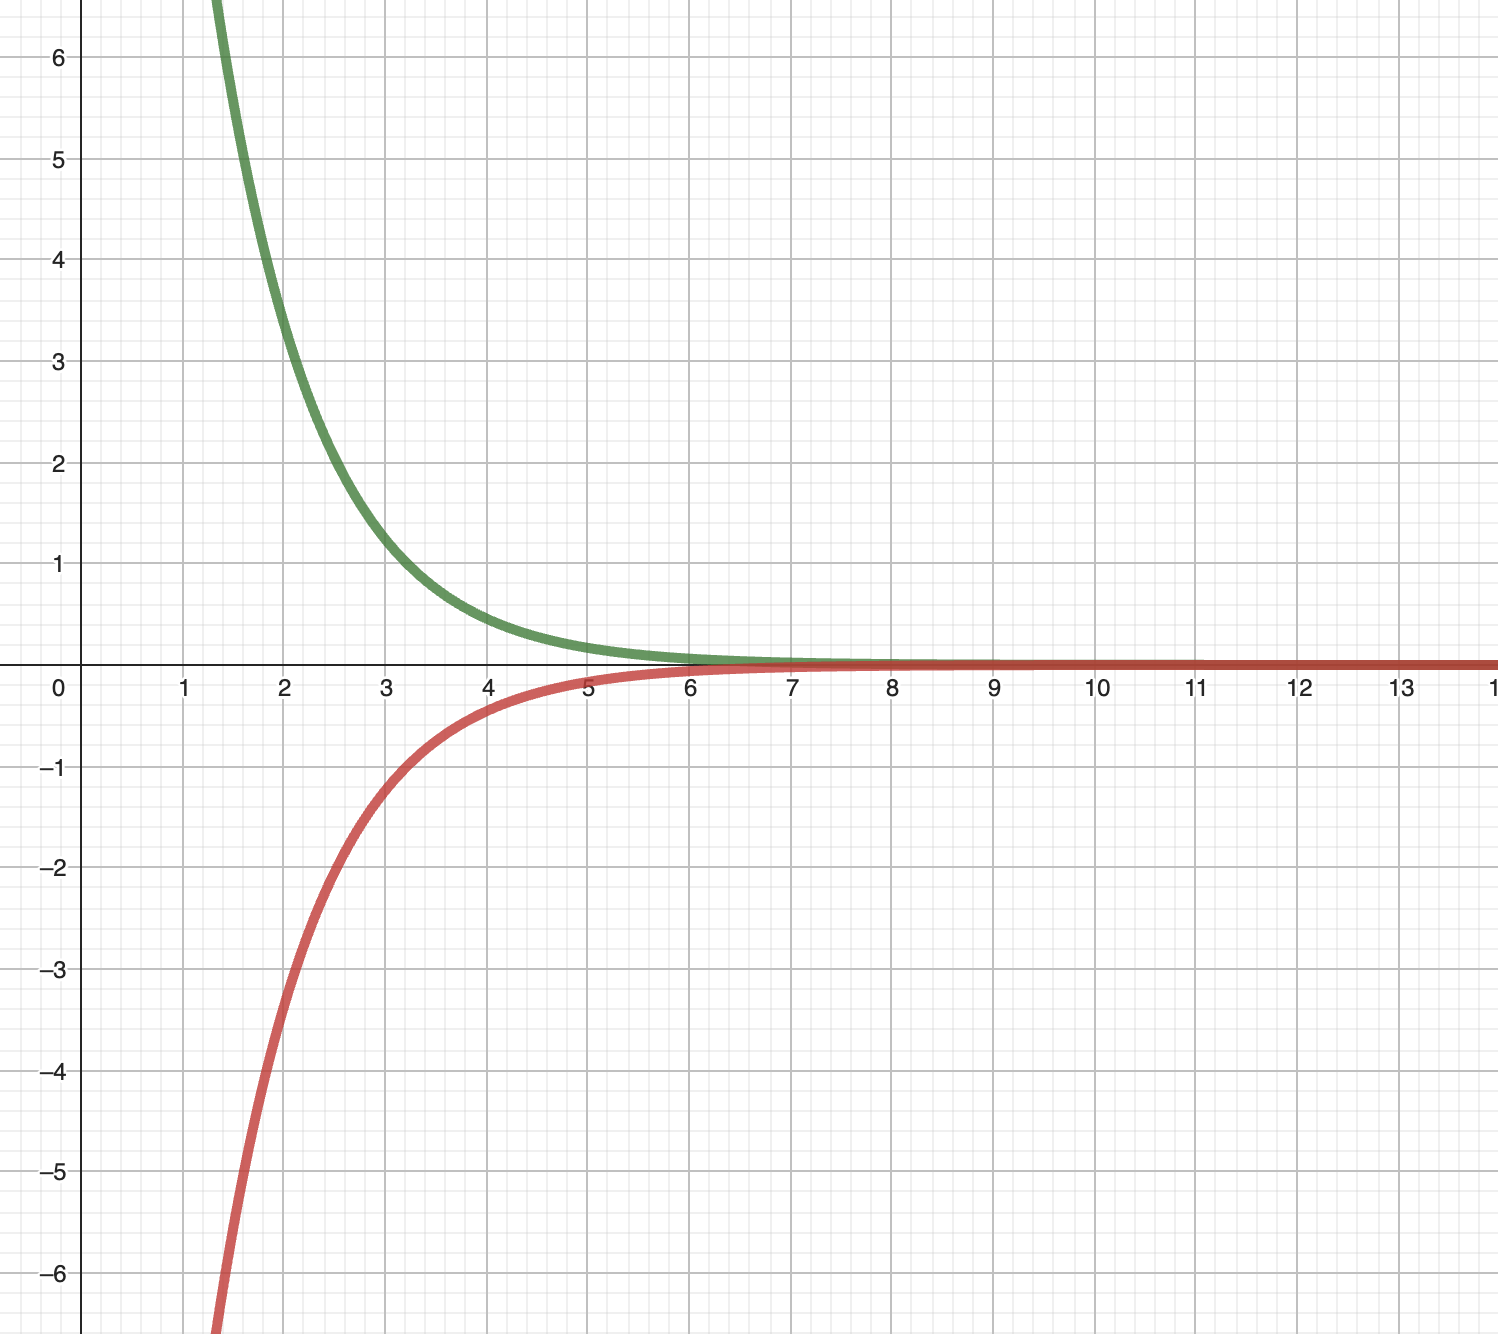
\includegraphics[width=1\linewidth]{./images/ratioLimits.png} 
\end{wrapfigure}

\noindent\textbf{NB!} Il caso descritto nel punto \textit{d)} non è indeterminato. Infatti $\frac{f}{g} = f\cdot\frac{1}{g} = \infty$ (il segno poi dipende a seconda di $f$ e di $g$).\\

\noindent\textbf{NB!} Dire che $\exists V_{x_0}$ intorno di $x_0$ tale che $g(x) > 0 \ (< 0) \qquad \forall x \in (V_{x_0} \cap A) - \{x_0\}$ significa dire che la funzione tende a $0$, mantenendo segno costante. Graficamente:

\subsubsection{Casi di indeterminazione}
Se $l_1 = l_2 = 0$ o $l_1 = l_2 = \pm\infty$, allora:

\begin{itemize}
    \item se $f(x) = x$ e $g(x) = x$, allora $$\lim_{x \to +\infty} f(x) = +\infty \quad \lim_{x \to +\infty} g(x) = + \infty \quad \lim_{x \to +\infty} \left(\dfrac{f}{g}\right)(x) = \lim_{x \to +\infty} 1 = 1$$
    \item se $f(x) = \frac{1}{x^2}$ e $g(x) = \frac{1}{x}$, allora $$\lim_{x \to +\infty} f(x) = 0 \quad \lim_{x \to +\infty} g(x) = 0 \quad \lim_{x \to +\infty} \left(\dfrac{f}{g}\right)(x) = \lim_{x \to +\infty} \left(\dfrac{1}{x}\right) = 0$$
    \item se $f(x) = x^2$ e $g(x) = x$, allora $$\lim_{x \to +\infty} f(x) = +\infty \quad \lim_{x \to +\infty} g(x) = +\infty \quad \lim_{x \to +\infty} \left(\dfrac{f}{g}\right)(x) = \lim_{x \to +\infty} x = +\infty$$
\end{itemize}

\noindent\textbf{Def:} Siano $A \neq \varnothing$ e $f: A \subset \mathbb{R} \xrightarrow{} \mathbb{R}$ e $x_0 \in \widetilde{\mathbb{R}}$ punto di accumulazione per $A$. \\
Se esiste $\lim_{x \to x_0} f(x) = l \in \mathbb{R}$ e $\exists V_{x_0} \ intorno \ di \ x_0 : f(x) > l \ (< l) \qquad \forall x \in (V_{x_0} \cap A) - \{x_0\} \overset{def}{\iff} \lim_{x \to x_0} f(x) = l^+ \ (l^-)$.\\

\noindent\textbf{NB!} Non si può scrivere che se $\lim_{x \to x_0} f(x) = 3$ e $\lim_{x \to x_0} f(x) = 2^+$, allora $\lim_{x \to x_0} (f + g)(x) = 5^+$ perché $2^+ \notin \mathbb{R}$. Infatti, se abbiamo $f(x) = 3 - x^2$, $g(x) = 2 + x ^4$ e $x_0 = 0$, allora $(f + g)(x) = 5 - x^2(x^2 - 1)$. Studiando ora il segno di $(f + g)(x)$, si ha che $x^2(x^2 - 1) < 0 : \ per \ x \in (-1, 1) - \{0\} \implies \lim_{x \to 0} (f + g)(x) = 5^-$ (perché $\lim_{x \to 0} x^2(x^2 - 1)$ tende a $0^-$.

\subsection{Intorni, punti di accumulazione e limiti destri e sinistri}
Sia $x_0 \in \mathbb{R}$ e $\delta > 0$, allora definiamo:

\begin{itemize}
    \item $D^+(x_0, \delta) = D(x_0, \delta) \cap \{x \in \mathbb{R} \ | \ x > x_0\}$ disco destro di centro $x_0$ e raggio $\delta$;
    \item $D^-(x_0, \delta) = D(x_0, \delta) \cap \{x \in \mathbb{R} \ | \ x < x_0\}$ disco sinistro di centro $x_0$ e raggio $\delta$;
\end{itemize}

\noindent\textbf{Osservazione:} $D^+(x_0, \delta) = (x_0, x_0 + \delta)$ e $D^-(x_0, \delta) = (x_0 - \delta, x_0)$.\\

\noindent\textbf{NB!} $x_0$ è escluso in questi intorni.\\

\noindent\textbf{Def: }Sia $x_0 \in \mathbb{R}$, $A \subseteq \mathbb{R}$, $A \neq \varnothing$. Diremo che $x_0$ è punto di accumulazione a destra (sinistra) per $A$ se e solo se $\forall \delta > 0$ si ha che:

\begin{equation*}
    D^+(x_0, \delta) \cap A \neq \varnothing \qquad (D^-(x_0, \delta) \cap A \neq \varnothing)
\end{equation*}

\noindent\textbf{NB!} È la stessa definizione di punto di accumulazione, ma abbiamo cambiato l'intorno bilatero con uno unilatero.\\

\noindent\textbf{ES.} Sia $A = (3, 4)$, allora:

\begin{itemize}
    \item $3$ è punto di accumulazione a destra, ma non a sinistra. Per questo motivo, non si può calcolare il limite a sinistra;
    \item $4$ è punto di accumulazione a sinistra, ma non a destra. Per questo motivo, non si può calcolare il limite a destra;
    \item $x \in (3, 4)$ sono punti di accumulazione sia a destra che a sinistra.
\end{itemize}

\noindent\textbf{Def:} Siano $A \neq \varnothing$, $f: A \subset \mathbb{R} \xrightarrow{} \mathbb{R}$ e $x_0 \in \mathbb{R}$ punto di accumulazione destro (sinistro) per $A$. Sia $l \in \widetilde{\mathbb{R}}$. Diremo che $f$ ammette limite $l$ per $x$ che tende a $x_0$ da destra (sinistra) se e solo se:
\begin{equation*}
    \forall V_l \ intorno \ di \ l, \exists U^+_{x_0} \ (U^-_{x_0}) \ intorno \ destro \ (sinistro) \ di \ x_0 \ | \ f(x) \in V_l \qquad \forall x \in U^+_{x_0} \cap A \ (U^-_{x_0} \cap A)
\end{equation*}

\noindent In tal caso, scriviamo:

\begin{equation*}
    \lim_{x \to x_0^+} f(x) = l \qquad \lim_{x \to x_0^-} f(x) = l
\end{equation*}

\noindent\textbf{Teorema:} Siano $f: A \subset \mathbb{R} \xrightarrow{} \mathbb{R}$, $A \neq \varnothing$ e $x_0 \in \mathbb{R}$ punto di accumulazione per $A$ (cioè sia a destra che a sinistra). Allora:

\begin{enumerate}[label=\alph{enumi})]
    \item se $\lim_{x \to x^+_0} f(x) = l_1 \in \widetilde{\mathbb{R}}$ e $\lim_{x \to x^-_0} f(x) = l_2 \in \widetilde{\mathbb{R}}$ con $l_1 = l_2 = l \implies \lim_{x \to x_0} f(x) = l$;
    \item se $\lim_{x \to x_0} f(x) = l \in \widetilde{\mathbb{R}} \implies \lim_{x \to x^+_0} f(x) = l$ e $\lim_{x \to x^-_0} = l$.
\end{enumerate}

\noindent\textbf{NB!} Un modo per mostrare che una funzione ammette limite è calcolare il limite destro e quello sinistro e poi verificare che essi siano uguali.\\

\noindent\textbf{Dimostrazione del punto a):} Per ipotesi sappiamo che:

\begin{itemize}
    \item $\forall V_l \ intorno \ di \ l, \exists \delta_1 > 0 \ per \ cui \ f(x) \in V_l \qquad \forall x \in A \cap (x_0, x_0 + \delta_1)$;
    \item $\forall V_l \ intorno \ di \ l, \exists \delta_2 > 0 \ per \ cui \ f(x) \in V_l \qquad \forall x \in A \cap (x_0 - \delta_2, x_0)$;
\end{itemize}

\noindent Chiamiamo allora $\delta = min(\delta_1, \delta_2)$. Allora $f(x) \in V_l \qquad \forall x \in (A \cap (x_0 - \delta, x_0 + \delta)) - \{x_0\}$, ossia è vero per la definizione di limite.\\

\noindent\textbf{Dimostrazione del punto b):} Per ipotesi sappiamo che:

\begin{equation*}
    \forall V_l \ intorno \ di \ l, \exists \delta > 0 \ per \ cui \ f(x) \in V_l \qquad \forall x \in A \cap (x_0 - \delta, x_0 + \delta) - \{x_0\}
\end{equation*}

\noindent quindi dividendo l'intorno $(x_0 - \delta, x_0 + \delta) - \{x_0\}$ in due parti otteniamo: $(x_0 - \delta, x_0)$ e $(x_0, x_0 + \delta)$. Per cui dall'ipotesi, possiamo dire che:

\begin{equation*}
    \forall V_l \ intorno \ di \ l, \exists \delta > 0 \ per \ cui \ f(x) \in V_l \qquad \forall x \in A \cap (x_0 - \delta, x_0) - \{x_0\} \implies \lim_{x \to x^-_0} f(x) = l
\end{equation*}
\begin{equation*}
    \forall V_l \ intorno \ di \ l, \exists \delta > 0 \ per \ cui \ f(x) \in V_l \qquad \forall x \in A \cap (x_0, x_0 + \delta) - \{x_0\} \implies \lim_{x \to x^+_0} f(x) = l
\end{equation*}

\noindent\textbf{ES.} Siano $A = \mathbb{R} - \{0\}$ e $f(x) = \frac{1}{x}$ e $x_0 = 0$ punto di accumulazione per $A$. Allora:

\begin{equation*}
    \lim_{x \to 0^+} \frac{1}{x} = +\infty \qquad \lim_{x \to 0^-} \frac{1}{x} = -\infty \qquad \nexists\lim_{x \to 0} \frac{1}{x} 
\end{equation*}

\noindent Perché per esistere, $\lim_{x \to x^+_0} = \lim_{x \to x^-_0} = l$.

\subsection{Teorema sui limiti delle funzioni monotone}
Siano $a, b \in \widetilde{\mathbb{R}}$ e $I = (a, b)$ (ogni volta che si parla di funzioni monotone, il dominio è un intervallo!) e $f: I \subset \mathbb{R} \xrightarrow{} \mathbb{R}$. Allora:

\begin{wrapfigure}{l}{0.4\textwidth}
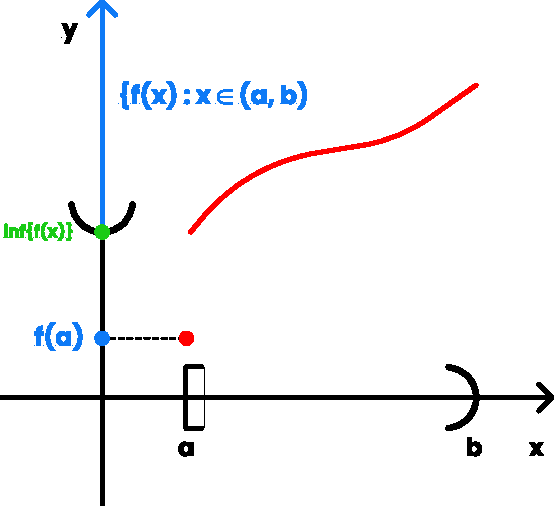
\includegraphics[width=0.7\linewidth]{images/monotonicFunctionsLimits.pdf} 
\vspace{-20pt}
\end{wrapfigure}

\begin{enumerate}[label=\alph{enumi})]
    \item se $f$ è debolmente crescente in $I$, allora: $$\lim_{x \to \underset{\scriptstyle (-\infty)}{a^+}} f(x) = inf\{f(x) : x \in (a, b)\}$$ $$\lim_{x \to \underset{\scriptstyle (+\infty)}{b^-}} f(x) = sup\{f(x) : x \in (a, b)\}$$ ovvero il limite destro di $a$ è uguale all'estremo inferiore dell'immagine e il limite sinistro di $b$ è uguale all'estremo superiore di $b$;
    \item se $f$ è debolmente decrescente in $I$, allora: $$\lim_{x \to \underset{\scriptstyle (-\infty)}{a^+}} f(x) = sup\{f(x) : x \in (a, b)\}$$ $$\lim_{x \to \underset{\scriptstyle (+\infty)}{b^-}} f(x) = inf\{f(x) : x \in (a, b)\}$$ ovvero il limite destro di $a$ è uguale all'estremo inferiore dell'immagine e il limite sinistro di $b$ è uguale all'estremo superiore di $b$;
\end{enumerate}

\noindent\textbf{NB!} Sia $J = [a, b)$, allora nell'intervallo dell'insieme immagine devo mettere $(a, b)$ oppure $[a, b)$? \\
Nella tesi continuo a mettere $(a, b)$, perché ci interessano, nel caso di $\lim_{x \to a^+} f(x)$, solo intorni destri di $a$ che quindi non comprendo $a$ stessa. \\
In altre parole, se cambiamo il dominio in $[a, b]$, $[a, b)$ o $(a, b]$, nella tesi va sempre messo $(a, b)$ perché nella definizione di limite il valore di $f(x_0)$ con $x_0 \in D_f$ e $x_0$ punto di accumulazione per $D_f$, è \textbf{escluso}. Potremmo infatti avere una funzione simile a questa di sinistra.

\subsubsection{Dimostrazione del teorema sui limiti delle funzioni monotone}
Se $f$ è debolmente crescente su $I$, significa che $(-f)$ è debolmente decrescente su $I$. Applichiamo ora $a)$ sulla funzione $(-f)$:

\begin{equation*}
    \lim_{x \to \underset{\scriptstyle (-\infty)}{a^+}} (-f)(x) = sup\{-f(x) : x \in (a, b) \ (x \in (-\infty, b))\}
\end{equation*}

\noindent Ora, dato che $\lim_{x \to \underset{\scriptstyle (-\infty)}{a^+}} (-f)(x) = - \lim_{x \to \underset{\scriptstyle (-\infty)}{a^+}} f(x)$ e che $sup(-A) = -inf(A)$, si ha che:

\begin{equation*}
    - \lim_{x \to \underset{\scriptstyle (-\infty)}{a^+}} f(x) = - inf(A) \implies \lim_{x \to \underset{\scriptstyle (-\infty)}{a^+}} f(x) = inf(A)
\end{equation*}

\noindent Dimostriamo ora che $\lim_{x \to \underset{\scriptstyle (+\infty)}{b^-}} f(x) = sup\{f(x) : x \in (a, b) \ (x \in (a, +\infty))\}$. Sappiamo che la funzione è monotona crescente ed è definita nell'intervallo $I = (a, b) \ ((a, + \infty))$. Sia ora $b \in \mathbb{R}$ e sia $\Lambda = sup\{f(x) : x \in (a, b) \ ((a, +\infty))\}$.\\
Ipotizziamo che $\Lambda \in \mathbb{R}$, allora si ha che $\forall \varepsilon > 0, \exists x_\varepsilon : f(x_\varepsilon) > \Lambda - \varepsilon$ per la caratterizzazione degli estremi superiori (ovvero $\Lambda - \varepsilon$, a differenza di $\Lambda$, non è un maggiorante). \\
Sia ora $x \in (x_\varepsilon, b) \ ((x_\varepsilon, +\infty))$. Dato che il dominio è un intervallo, siamo certi che $x$ sta in esso (visto che $x_\varepsilon > a$). Possiamo quindi calcolare $f(x)$. Inoltre, sappiamo che $x_\varepsilon < x < b \ (x_\varepsilon < x)$. Quindi:

\begin{itemize}
    \item per definizione data precedentemente, sappiamo che $\Lambda - \varepsilon < f(x_\varepsilon)$;
    \item dato che $f(x)$ è una funzione strettamente crescente, si ha che $f(x_\varepsilon) \leq f(x)$;
    \item dato che $\Lambda$ è un maggiorante di $f$ (in particolare, è il minimo dei maggioranti), allora $f(x) \leq \Lambda$;
    \item sappiamo sicuramente che $\Lambda < \Lambda + \varepsilon$.
\end{itemize}

\noindent Unendo tutte queste condizioni otteniamo la seguente catena di disuguaglianze:
\begin{equation*}
    \Lambda - \varepsilon < f(x_\varepsilon) \leq f(x) \leq \Lambda < \Lambda + \varepsilon
\end{equation*}

\noindent e dimenticandoci di alcune parti di essa, possiamo vedere proprio che $\Lambda - \varepsilon < f(x) < \Lambda + \varepsilon$. Cioè otteniamo che:
\begin{equation*}
    \forall \varepsilon > 0, \exists x_\varepsilon \in I : |f(x) - \Lambda| < \varepsilon \qquad \forall x \in (x_\varepsilon, b) \ (\forall x \in (x_\varepsilon, +\infty))
\end{equation*}

\noindent Poniamo ora $\delta_\varepsilon = b - x_\varepsilon > 0$ e quindi $x_\varepsilon = b - \delta_\varepsilon$, allora possiamo riscrivere la precedente definizione come: 
\begin{equation*}
    \forall \varepsilon > 0, \exists x_\varepsilon \in I : |f(x) - \Lambda| < \varepsilon \qquad \forall x \in (b - \delta_\varepsilon, b) \implies \lim_{x \to \underset{\scriptstyle (+\infty)}{b^-}} f(x) = \Lambda
\end{equation*}

\noindent dove $(b - \delta_\varepsilon, b)$ rappresenta proprio un intorno sinistro.\\

\noindent Se invece avessimo avuto $\Lambda = +\infty$ (non si studia il caso in cui $\Lambda = -\infty$, altrimenti non potrebbe sicuramente essere $sup(A)$) e $b \in \mathbb{R} \ (b = +\infty)$, essendo $\Lambda = + \infty$, $Imm(f)$ non sarebbe stata superiormente limitata, per cui $\forall K \in \mathbb{R}, \exists x_K \in I : f(x_K) > K$.\\
Sia ora $x \in (x_K, b) \subset I \ ((x \in (x_K, +\infty) \subset I))$, dove $I$ è un intervallo, dato che $x > x_K$, allora: 
\begin{equation*}
    K < f(x_K) \leq f(x)
\end{equation*}

\noindent (abbiamo messo "$\leq$" e non "$<$" perché la funzione è debolmente (non strettamente) crescente) e quindi $\forall K \in \mathbb{R}, \exists x_K \in I : f(x) > K \qquad \forall x \in (x_K, b) \ ((\forall x \in (x_K, +\infty))$. Se $\delta_K = b - x_K \implies x_K = b - \delta_K$ e quindi: 
\begin{equation*}
    \forall K \in \mathbb{R}, \exists x_K \in I : f(x) > K \qquad \forall x \in (b - \delta_K, b) \ ((\forall x \in (x_K, +\infty)) \implies \lim_{x \to \underset{\scriptstyle (+\infty)}{b^-}} f(x) = +\infty
\end{equation*}

\noindent Allo stesso modo, se $f$ è debolmente decrescente su $I$, significa che $(-f)$ è debolmente crescente su $I$. Applichiamo ora $a)$ sulla funzione $(-f)$:

\begin{equation*}
    \lim_{x \to \underset{\scriptstyle (-\infty)}{a^+}} (-f)(x) = inf\{-f(x) : x \in (a, b) \ (x \in (-\infty, b))\}
\end{equation*}

\noindent Ora, dato che $\lim_{x \to \underset{\scriptstyle (-\infty)}{a^+}} (-f)(x) = - \lim_{x \to \underset{\scriptstyle (-\infty)}{a^+}} f(x)$ e che $inf(-A) = -sup(A)$, si ha che:

\begin{equation*}
    - \lim_{x \to \underset{\scriptstyle (-\infty)}{a^+}} f(x) = - sup(A) \implies \lim_{x \to \underset{\scriptstyle (-\infty)}{a^+}} f(x) = sup(A)
\end{equation*}

\noindent Dimostriamo ora che $\lim_{x \to \underset{\scriptstyle (+\infty)}{b^-}} f(x) = inf\{f(x) : x \in (a, b) \ (x \in (a, +\infty))\}$. Sappiamo che la funzione è monotona decrescente ed è definita nell'intervallo $I = (a, b)$. Sia ora $b \in \mathbb{R}$ e sia $\Lambda = inf\{f(x) : x \in (a, b) \ (x \in (a, +\infty))\}$.\\
Ipotizziamo che $\Lambda \in \mathbb{R}$, allora si ha che $\forall \varepsilon > 0, \exists x_\varepsilon : f(x_\varepsilon) < \Lambda + \varepsilon$ per la caratterizzazione degli estremi superiori (ovvero $\Lambda + \varepsilon$, a differenza di $\Lambda$, non è un minorante). \\
Sia ora $x \in (x_\varepsilon, b) \ ((x_\varepsilon, +\infty))$. Dato che il dominio è un intervallo, siamo certi che $x$ sta in esso (visto che $x_\varepsilon > a$). Possiamo quindi calcolare $f(x)$. Inoltre, sappiamo che $x_\varepsilon < x < b \ (x_\varepsilon < x)$. Quindi:

\begin{itemize}
    \item per definizione data precedentemente, sappiamo che $f(x_\varepsilon) < \Lambda + \varepsilon$;
    \item dato che $f(x)$ è una funzione strettamente decrescente, si ha che $f(x) \leq f(x_\varepsilon)$;
    \item dato che $\Lambda$ è un minorante di $f$ (in particolare, è il massimo dei minoranti), allora $\Lambda \leq f(x)$;
    \item sappiamo sicuramente che $\Lambda < \Lambda + \varepsilon$.
\end{itemize}

\noindent Unendo tutte queste condizioni otteniamo la seguente catena di disuguaglianze:
\begin{equation*}
    \Lambda - \varepsilon < \Lambda \leq f(x) \leq f(x_\varepsilon) < \Lambda + \varepsilon
\end{equation*}

\noindent e dimenticandoci di alcune parti di essa, possiamo vedere proprio che $\Lambda - \varepsilon < f(x) < \Lambda + \varepsilon$. Cioè otteniamo che:
\begin{equation*}
    \forall \varepsilon > 0, \exists x_\varepsilon \in I : |f(x) - \Lambda| < \varepsilon \qquad \forall x \in (x_\varepsilon, b) \ (\forall x \in (x_\varepsilon, +\infty))
\end{equation*}

\noindent Poniamo ora $\delta_\varepsilon = b - x_\varepsilon > 0$ e quindi $x_\varepsilon = b - \delta_\varepsilon$, allora possiamo riscrivere la precedente definizione come: 
\begin{equation*}
    \forall \varepsilon > 0, \exists x_\varepsilon \in I : |f(x) - \Lambda| < \varepsilon \qquad \forall x \in (b - \delta_\varepsilon, b) \implies \lim_{x \to b^-} f(x) = \Lambda
\end{equation*}

\noindent dove $(b - \delta_\varepsilon, b)$ rappresenta proprio un intorno sinistro.\\

\noindent Se invece avessimo avuto $\Lambda = -\infty$ (non si studia il caso in cui $\Lambda = +\infty$, altrimenti non potrebbe sicuramente essere $inf(A)$) e $b \in \mathbb{R} \ (b = +\infty)$, essendo $\Lambda = - \infty$, $Imm(f)$ non sarebbe stata inferiormente limitata, per cui $\forall K \in \mathbb{R}, \exists x_K \in I : f(x_K) < K$.\\
Sia ora $x \in (x_K, b) \subset I \ ((x \in (x_K, +\infty) \subset I))$, dove $I$ è un intervallo, dato che $x < x_K$, allora: 
\begin{equation*}
    f(x) \leq f(x_K) < K
\end{equation*}

\noindent (abbiamo messo "$\leq$" e non "$<$" perché la funzione è debolmente (non strettamente) decrescente) e quindi $\forall K \in \mathbb{R}, \exists x_K \in I : f(x) < K \qquad \forall x \in (x_K, b)$. Se $\delta_K = b - x_K \implies x_K = b - \delta_K$ e quindi: 
\begin{equation*}
    \forall K \in \mathbb{R}, \exists x_K \in I : f(x) < K \qquad \forall x \in (b - \delta_K, b) \ ((\forall x \in (x_K, +\infty)) \implies \lim_{x \to \underset{\scriptstyle (+\infty)}{b^-}} f(x) = -\infty
\end{equation*}

\subsection{Limiti di esponenziali e logaritmi}
\textbf{Teorema:} Sia $a > 0$ con $a \neq 1$. Allora:

\begin{enumerate}
    \item se $a > 1$, allora si ha che: $$\lim_{x \to - \infty} a^x = 0^+ \qquad \lim_{x \to +\infty} a^x = +\infty$$
    \item se $0 < a < 1$, allora si ha che: $$\lim_{x \to - \infty} a^x = +\infty \qquad \lim_{x \to +\infty} a^x = 0^+$$
    \item se $a > 1$, allora si ha che: $$\lim_{x \to 0^+} \log_ax = -\infty \qquad \lim_{x \to +\infty} \log_ax = + \infty$$
    \item se $0 < a < 1$, allora si ha che: $$\lim_{x \to 0^+} \log_ax = +\infty \qquad \lim_{x \to +\infty} \log_ax = -\infty$$
\end{enumerate}

\noindent\textbf{NB!} $a = 1$ è escluso perché $1^x = 1 \qquad \forall x \in \mathbb{R}$.

\subsubsection{Dimostrazione dei limiti di esponenziali e logaritmi}
Sia $a > 1$. $a^x$ è strettamente crescente su $\mathbb{R}$, allora per il teorema sui limiti di funzioni monotone:
\begin{equation*}
    \lim_{x \to -\infty} a^x = inf\{f(x) : x \in \mathbb{R}\} \qquad \lim_{x \to +\infty} a^x = sup\{f(x) : x \in \mathbb{R}\}
\end{equation*}

\noindent Se l'immagine di $a^x$ non è superiormente limitata, allora il risultato del limite sarà $+\infty$. In altre parole, se riusciamo a mostrare che un sottoinsieme dell'immagine non è superiormente limitato, allora nemmeno l'insieme immagine lo è. \\
Siccome $a > 1$, chiamo $b = a - 1 > 0$, allora per la disuguaglianza di Bernoulli, si ha che $a^n = (1 + b)^n \geq 1 + nb$. Dato che $1 + nb$ non è superiormente limitato (perché $\lim_{n \to +\infty} 1 + nb = +\infty$), possiamo utilizzare il teorema del confronto per dire che $\lim_{n \to +\infty} a^n = +\infty$. Quindi $\{(1 + b)^n = a^n : n \in \mathbb{N}\}$ non è superiormente limitato, ovvero $\{(1 + b)^n = a^n : n \in \mathbb{N}\} = + \infty$.\\
Dato però che $\{(1 + b)^n = a^n : n \in \mathbb{N}\} \subset \{(1 + b)^x = a^x : x \in \mathbb{R}\}$, allora nemmeno $\{(1 + b)^x = a^x : x \in \mathbb{R}\}$ è superiormente limitato, ovvero $\{(1 + b)^x = a^x : x \in \mathbb{R}\} = +\infty$. Quindi $\lim_{x \to +\infty} a^x = + \infty \quad \ con \ a > 1$.\\
Ora dimostriamo che $\lim_{x \to - \infty} a^x = 0^+$. Innanzitutto, sappiamo che $\lim_{x \to - \infty} a^x = inf\{f(x) : x \in \mathbb{R}\}$ per il teorema sui limiti di funzioni monotone. Inoltre, nel punto precedente abbiamo dimostrato che $\lim_{n \to +\infty} a^n = +\infty$, allora $\lim_{n \to +\infty} a^{-n} = \lim_{n \to +\infty} \frac{1}{a^n} = 0$ per il limite del rapporto.\\
Siccome $a^{-n}$ è strettamente decrescente, si ha che:
\begin{equation*}
    0 = \lim_{n \to +\infty} a^{-n} = inf\{a^{-n} : n \in \mathbb{N}\}
\end{equation*}
Ma $\{a^{-n} : n \in \mathbb{N}\} \subsetneq \{a^x : x \in \mathbb{R}\}$. Usando poi il fatto che $A \subset B \implies inf(A) \geq inf(B)$ (\textit{Esercizio 1} di questo pdf), si ottiene che:
\begin{equation*}
    0 = inf\{a^{-n} : n \in \mathbb{N}\} \geq inf\{a^x : x \in \mathbb{R}\}
\end{equation*}

\noindent A questo punto, dato che $a^x > 0 \qquad \forall x \in \mathbb{R}$ (significa che non ci sono numeri più piccolo dello zero e quindi che $0$ è un minorante), possiamo utilizzare il teorema del confronto e dire che:
\begin{equation*}
    0 \geq inf\{a^x : x \in \mathbb{R}\} = \lim_{x \to -\infty} a^x \geq \lim_{x \to -\infty} 0 = 0
\end{equation*}

\noindent Quindi $0 \geq \lim_{x \to -\infty} a^x \leq 0 \implies \lim_{x \to -\infty} a^x = 0^+ \quad con \ a > 1; a^x > 0 \quad \forall x \in \mathbb{R}$.\\
Sia ora $0 < a < 1$, allora $c = \frac{1}{a} > 1$. Sappiamo per il punto 1) che:
\begin{equation*}
    \lim_{x \to -\infty} c^x = 0^+ \qquad \lim_{x \to +\infty} c^x = +\infty
\end{equation*}

\noindent Quindi per il limite del rapporto, si ha che:
\begin{equation*}
    \lim_{x \to -\infty} a^x = \lim_{x \to -\infty} \frac{1}{\frac{1}{a^x}} = \lim_{x \to -\infty} \frac{1}{c^x} = +\infty \qquad \lim_{x \to +\infty} a^x = \lim_{x \to +\infty} \frac{1}{\frac{1}{a^x}} = \lim_{x \to +\infty} \frac{1}{c^x} = 0^+
\end{equation*}

\noindent Dimostriamo ora i punti 3. e 4. Innanzitutto, ricordiamo che $\log_ax = (a^x)^{-1}$ (ovvero che il logaritmo è l'operazione inversa dell'esponenziale), allora se $a > 1$, $\log_ax$ è strettamente crescente (questo perché in un precedente teorema avevamo detto che se una funzione è strettamente crescente (decrescente), allora anche l'inversa lo è), per cui:
\begin{equation*}
    \lim_{x \to 0^+} \log_ax = inf\{Imm(\log_ax)\} = inf\{Dom(a^x)\} = inf\{\mathbb{R}\} = - \infty
\end{equation*}
\begin{equation*}
    \lim_{x \to +\infty} \log_ax = sup\{Imm(\log_ax)\} = sup\{Dom(a^x)\} = sup\{\mathbb{R}\} = + \infty
\end{equation*}

\noindent Se invece $0 < a < 1$, allora $\log_ax$ è strettamente decrescente, per cui:
\begin{equation*}
    \lim_{x \to 0^+} \log_ax = sup\{Imm(\log_ax)\} = sup\{Dom(a^x)\} = sup\{\mathbb{R}\} = + \infty
\end{equation*}
\begin{equation*}
    \lim_{x \to +\infty} \log_ax = inf\{Imm(\log_ax)\} = inf\{Dom(a^x)\} = inf\{\mathbb{R}\} = - \infty
\end{equation*}

\noindent\textbf{NB!} Abbiamo quindi trovato gli \textbf{estremi del campo di esistenza} ovvero i punti di accumulazione non appartenenti al dominio massimale. Ad esempio, $Dom(\log_ax) = (0, +\infty)$, allora questi punti sono $x_0 = 0$ e $x_0 = +\infty$.

\subsection{Teorema sui limiti per sostituzione}
Cosa succede se devo studiare un limite di una composizione di funzioni, come ad esempio $\lim_{t \to +\infty} 2^\frac{1}{t^2}$?\\
In questo caso, infatti, si ha una catena di composizione del tipo:
\begin{equation*}
    t \longmapsto t^2 \longmapsto \frac{1}{t^2} \longmapsto 2^\frac{1}{t^2}
\end{equation*}

\noindent È proprio in questi casi quindi che si parla di limiti per sostituzione, ovvero di limiti in cui si cerca di ricondursi a funzioni di cui conosciamo già i valori dei limiti. Ad esempio, conosciamo i valori di:
\begin{equation*}
    \lim_{u \to +\infty} u^2 = +\infty \qquad \lim_{w \to +\infty} \frac{1}{w} = 0^+ \qquad \lim_{s \to 0^+} 2^s
\end{equation*}

\noindent\textbf{Teorema:} Sia $f: A \subset \mathbb{R} \xrightarrow{} \mathbb{R}$ e sia $x_0 \in \widetilde{\mathbb{R}}$ punto di accumulazione per $A$. Assumiamo che $\lim_{x \to x_0} f(x) = l \in \widetilde{\mathbb{R}}$ (dove $f(x)$ rappresenta la funzione più esterna di tutte). Siano inoltre $B \neq \varnothing$, $\varphi: B \subset \mathbb{R} \xrightarrow{} A$ (dato che $\varphi$ rappresenta la prima funzione della nostra composizione, è fondamentale che il suo codominio sia contenuto nel dominio della funzione finale $f(x)$), $t_0 \in \widetilde{\mathbb{R}}$ punto di accumulazione per $B$. Assumiamo, inoltre, che $\lim_{t \to t_0} \varphi(t) = x_0$ (nell'esempio di prima $x_0 = 0^+$ e $\varphi(t) = \frac{1}{t^2}$) e che valga almeno una delle seguenti ipotesi:

\begin{enumerate}
    \item $\varphi(t) \neq x_0 \qquad \forall t \in B, t \neq t_0$;
    \item $x_0 \in A$ e $f(x_0) = l$ e quindi $l \in \mathbb{R}$
\end{enumerate}

\noindent allora $\lim_{t \to t_0} f(\varphi(t)) = l$, dove ($f(\varphi(t))$ sarebbe $2^\frac{1}{t^2}$ nell'esempio di prima; in pratica, il valore del limite diventa il punto di accumulazione del limite successivo). \\
In pratica, l'assunzione $\lim_{t \to t_0} \varphi(t) = x_0$ ci sta dicendo che $\varphi(t)$ appartiene ad intorni di $x_0$ e, l'ipotesi 1., aggiunge che si tratta di intorni bucati, dato che $x_0$ non appartiene all'insieme immagine. L'ipotesi 2., invece, dice che la funzione esterna vale in intorni pieni, ovvero che è possibile calcolare $f(x_0)$.

\subsubsection{Dimostrazione del teorema sui limiti per sostituzione}
Sia $l \in \mathbb{R}$, per definizione allora:
\begin{equation*}
    \lim_{x \to x_0} f(x) = l \iff \forall \varepsilon > 0, \exists U_{x_0} \ intorno \ di \ x_0 \ tale \ che \ |f(x) - l| < \varepsilon \qquad \forall x \in (U_{x_0} \cap A) - \{x_0\}
\end{equation*}

\noindent Inoltre, sappiamo che:
\begin{equation*}
    \lim_{t \to t_0} \varphi(t) = x_0 \iff \forall V_{x_0}, \exists W_{t_0} \ intorno \ di \ t_0 \ tale \ che \ \varphi(t) \in V_{x_0} \qquad \forall t \in (W_{t_0} \cap B) - \{t_0\}
\end{equation*}

\noindent Dato che $\varphi(t) \in V_{x_0}$ per la definizione qui sopra e che il nostro obiettivo è fare la composizione di funzioni $f(\varphi(t))$ per cui $\varphi(t) \in A$ (ovvero l'insieme immagine di $\varphi$ deve essere contenuto nel dominio di $f$, cioè $A$), possiamo scrivere: $\varphi(t) \in (V_{x_0} \cap A) \qquad \forall t \in (W_{t_0} \cap B) - \{t_0\}$.\\
Ora siccome abbiamo arbitrarietà nella scelta di $V_{x_0}$, scegliamo $V_{x_0} \vcentcolon = U_{x_0}$. Di conseguenza:
\begin{equation*}
    \varphi(t) \in (U_{x_0} \cap A) \qquad \forall t \in (W_{t_0} \cap B) - \{t_0\}
\end{equation*}

\noindent (ora quindi la differenza tra $f$ e $\varphi$ è che $f$ sta in un intorno bucato di $x_0$ per la definizione del suo limite, mentre $\varphi$ sta in un intorno di $x_0$).\\
Se vale l'\textit{ipotesi 1.}, allora possiamo concludere che:
\begin{equation*}
    \varphi(t) \in (U_{x_0} \cap A) - \{x_0\} \qquad \forall t \in (W_{t_0} \cap B) - \{t_0\}
\end{equation*}

\noindent e quindi che:
\begin{equation*}
    \forall \varepsilon > 0, \exists W_{t_0} \ intorno \ di \ t_0 : |f(\varphi(t)) - l| < \varepsilon \qquad \forall t \in (W_{t_0} \cap B) - \{t_0\} \implies \lim_{t \to t_0} f(\varphi(t)) = l
\end{equation*}

\noindent Se vale invece l'\textit{ipotesi 2.}, allora abbiamo che $\lim_{x \to x_0} f(x) = l$ e $f(x_0) = l$. Quindi:
\begin{equation*}
    \forall \varepsilon > 0, \exists U_{x_0} \ intorno \ di \ x_0 : |f(x) - l| < \varepsilon \qquad \forall x \in (U_{x_0} \cap A)
\end{equation*}

\noindent (ovvero non dobbiamo togliere $x_0$ dall'intorno $U_{x_0}$). Usando ora di nuovo $\lim_{t \to t_0} \varphi(t) = x_0$ e la scelta $V_{x_0} \vcentcolon = U_{x_0}$ otteniamo che $\varphi(t) \in (U_{x_0} \cap A) \qquad \forall t \in (W_{t_0} \cap B) - \{t_0\}$.\\
Quindi:
\begin{equation*}
    \forall \varepsilon > 0, \exists W_{t_0} \ intorno \ di \ t_0 : |f(\varphi(t)) - l| < \varepsilon \qquad \forall t \in (W_{t_0} \cap B) - \{t_0\} \implies \lim_{t \to t_0} f(\varphi(t)) = l
\end{equation*}

\noindent Sia $l = +\infty \ (-\infty)$, allora per definizione:
\begin{equation*}
    \lim_{x \to x_0} f(x) = +\infty \iff \forall K > 0, \exists U_{x_0} \ intorno \ di \ x_0 \ tale \ che \ f(x) > K \qquad \forall x \in (U_{x_0} \cap A) - \{x_0\}
\end{equation*}
\begin{equation*}
    \lim_{x \to x_0} f(x) = -\infty \iff \forall K < 0, \exists U_{x_0} \ intorno \ di \ x_0 \ tale \ che \ f(x) < K \qquad \forall x \in (U_{x_0} \cap A) - \{x_0\}
\end{equation*}

\noindent Inoltre, sappiamo che:
\begin{equation*}
    \lim_{t \to t_0} \varphi(t) = x_0 \iff \forall V_{x_0}, \exists W_{t_0} \ intorno \ di \ t_0 \ tale \ che \ \varphi(t) \in V_{x_0} \qquad \forall t \in (W_{t_0} \cap B) - \{t_0\}
\end{equation*}

\noindent Dato che $\varphi(t) \in V_{x_0}$ per la definizione qui sopra e che il nostro obiettivo è fare la composizione di funzioni $f(\varphi(t))$ per cui $\varphi(t) \in A$ (ovvero l'insieme immagine di $\varphi$ deve essere contenuto nel dominio di $f$, cioè $A$), possiamo scrivere: $\varphi(t) \in (V_{x_0} \cap A) \qquad \forall t \in (W_{t_0} \cap B) - \{t_0\}$.\\
Ora siccome abbiamo arbitrarietà nella scelta di $V_{x_0}$, scegliamo $V_{x_0} \vcentcolon = U_{x_0}$. Di conseguenza:
\begin{equation*}
    \varphi(t) \in (U_{x_0} \cap A) \qquad \forall t \in (W_{t_0} \cap B) - \{t_0\}
\end{equation*}

\noindent (ora quindi la differenza tra $f$ e $\varphi$ è che $f$ sta in un intorno bucato di $x_0$ per la definizione del suo limite, mentre $\varphi$ sta in un intorno di $x_0$).\\
Se vale l'\textit{ipotesi 1.}, allora possiamo concludere che:
\begin{equation*}
    \varphi(t) \in (U_{x_0} \cap A) - \{x_0\} \qquad \forall t \in (W_{t_0} \cap B) - \{t_0\}
\end{equation*}

\noindent e quindi che:
\begin{equation*}
    \forall K > 0, \exists W_{t_0} \ intorno \ di \ x_0 : f(\varphi(t)) > K \qquad \forall t \in (W_{t_0} \cap B) - \{t_0\} \implies \lim_{t \to t_0} f(\varphi(t)) = +\infty
\end{equation*}
\begin{equation*}
    \forall K < 0, \exists W_{t_0} \ intorno \ di \ x_0 : f(\varphi(t)) < K \qquad \forall t \in (W_{t_0} \cap B) - \{t_0\} \implies \lim_{t \to t_0} f(\varphi(t)) = -\infty
\end{equation*}

\noindent\textbf{NB!} Non ha senso considerare l'\textit{ipotesi 2.} in questo caso perché quest'ultima vale solo se $l \in \mathbb{R}$.\\

\noindent\textbf{ES.} Siano:
\begin{equation*}
    f =
    \begin{cases}
       0 \quad se \ x \neq 0\\
       1 \quad se \ x = 0
    \end{cases}
\end{equation*}

\noindent $\varphi(t) = 0 \qquad \forall t \in \mathbb{R}, x_0 = 0, t_0 = 0$.\\
Allora si ha che:
\begin{equation*}
    \lim_{x \to 0} f(x) = 0 \ \forall x \neq 0 \qquad \lim_{t \to 0} f(\varphi(t)) = \lim_{t \to 0} f(0) = 1 \ \forall t \in \mathbb{R}
\end{equation*}

\noindent I limiti non risultano equivalenti, infatti né l'\textit{ipotesi 1.} (per essere vera dovremmo avere $\varphi(t) \neq x_0 \implies \varphi(t) \neq 0$, mentre qui abbiamo proprio che $\varphi(t) = x_0 = 0$), né l'\textit{ipotesi 2.} (la funzione $f$ è calcolabile in $x_0 = 0$, ma non vale $l$) risultano verificate.\\

\noindent\textbf{ES.} Calcolare $\lim_{t \to 0} 2^\frac{1}{t^2}$, in cui abbiamo che $x \overset{f}{\xrightarrow{}} 2^x$ e $t \overset{\varphi}{\xrightarrow{}} \frac{1}{t^2}$.\\
In altre parole, vogliamo usare il teorema di sostituzione "ponendo $x = \frac{1}{t^2}$", così possiamo usare $\lim_{x \to x_0} 2^x$. Ma chi è $x_0$?\\
Osservo che $\lim_{t \to 0} \frac{1}{t^2} = +\infty$ per il limite del rapporto. Pertanto abbiamo ricondotto il problema a $\lim_{x \to +\infty} 2^x = +\infty$. \\
Ora ci chiediamo, può valere l'\textit{ipotesi 2.}? No, perché $x_0 \notin \mathbb{R}$.\\
Può valere l'\textit{ipotesi 1.}? Sì, è certamente vera perché $\varphi(t) \neq x_0 \qquad \forall t \in B, t \neq t_0$ con $x_0 = +\infty$.\\
Allora per il teorema sui limiti per sostituzione:
\begin{equation*}
    \lim_{t \to 0} 2^\frac{1}{t^2} = \lim_{x \to +\infty} 2^x = +\infty
\end{equation*}

\subsection{Successioni}
Una successione è un'applicazione del tipo $f: A \subset \mathbb{N} \xrightarrow{} \mathbb{R}$. 

\subsubsection{Notazioni per scrivere successioni}
\begin{itemize}
    \item $a: A \subset \mathbb{N} \xrightarrow{} \mathbb{R} \qquad n \longmapsto a(n)$
    \item $\{a(n) : n \in A\}$
    \item $\{a_n : n \in A\}$
    \item $\{a_n\}_{n \in A}$
    \item $a_n, n \in A$
\end{itemize}

\noindent\textbf{ES.} Un esempio di successione può essere $f: \mathbb{N} - \{0\} \xrightarrow{} \mathbb{R} \qquad n \longmapsto \frac{1}{n}$ e può essere anche scritta come $\{\frac{1}{n} : n \geq 1\}$ o $\frac{1}{n}, n \geq 1$.

\subsubsection{Punti di accumulazione in $\mathbb{N}$}
\begin{itemize}
    \item $-1$, così come $x < 0, x \in \mathbb{R}$, non può essere un punto di accumulazione per $\mathbb{N}$ perché possiamo sempre trovare un $x +\delta < 0$ (per cui $(D(x, \delta) \cap \mathbb{N}) = \varnothing$);
    \item Nemmeno $x = 0$ va bene perché se prendiamo per esempio $D(m, \frac{1}{2})$, si ha che $(D(0, \frac{1}{2}) \cap \mathbb{N}) = \varnothing$;
    \item Neanche $m \in \mathbb{N}$ può andare bene perché, allo stesso modo di prima, se prendiamo come intorno $D(m, \frac{1}{2})$, l'intersezione tra questo e l'insieme dei numeri naturali risulta ancora essere vuota;
    \item Anche prendendo $x > 0, x \in \mathbb{R}$ non risolviamo il nostro problema. Infatti, questo numero $x$ sarà sicuramente compreso tra la sua parte intera e il numero successivo a questa. In simboli: $\lfloor x \rfloor < x < \lfloor x \rfloor + 1$. Per cui basterà prendere come raggio la metà della minima distanza tra un numero intero e l'altro, in simboli: $\delta = \frac{min(\Delta_1, \Delta_2)}{2}$ (dove $\Delta_1$ è la distanza tra $\lfloor x \rfloor$ e $x$, mentre $\Delta_2$ è la distanza tra $\lfloor x \rfloor + 1$ e $x$).
    \item Se invece prendiamo $x_0 = +\infty$, allora abbiamo un intorno del tipo $(K, +\infty)$. Quindi per la proprietà di Archimede, avremo sicuramente dei numeri naturali maggiori di $K$ (anche perché se non fosse così, significherebbe che $\mathbb{N}$ è superiormente limitato). Per cui otteniamo che $((K, + \infty) \cap \mathbb{N}) \neq \varnothing$ e che $x_0 = +\infty$ è un punto di accumulazione per $\mathbb{N}$.
\end{itemize}

\noindent Capiamo quindi che l'unico limite che possiamo calcolare quando siamo in presenza di una successione è il limite per $n$ che tende a $+\infty$.\\

\noindent Ne deriva inoltre il fatto che se abbiamo $A \subset \mathbb{N}$, con $A$ contenente finiti punti, allora $A$ non ha punti di accumulazione perché per qualsiasi punto $x_0$ preso, sia che $x_0 < 0$, sia che $x_0 \geq 0$, sarà sempre possibile prendere un raggio abbastanza piccolo tale che $D(x, \delta) \cap A = \varnothing$. Supponiamo per esempio che $A = (2, 7) \in \mathbb{N}$, allora se $x_0 = 2$, ma $\delta = \frac{1}{2}$ allora $D(x_0, \delta) \cap A = \varnothing$; se, per esempio, $4 < x_0 < 5$, allora se $\delta = \frac{min(\Delta_1, \Delta_2)}{2}$ (dove $\Delta_1$ è la distanza tra $\lfloor x \rfloor$ e $x$, mentre $\Delta_2$ è la distanza tra $\lfloor x \rfloor + 1$ e $x$), si ha che $D(x_0, \delta) \cap A = \varnothing$; se invece $x_0 < 2$ o $x_0 > 7$, allora basta prendere rispettivamente un $\delta < 2 - x_0$ o $\delta < x_0 - 7$.\\

\noindent\textbf{ES.} Dimostriamo che $\lim_{n \to +\infty} = 0$.\\
Ciò significa che:
\begin{equation*}
    \forall \varepsilon > 0, \exists K_\varepsilon \in \mathbb{R} : \left|\frac{1}{n} - 0\right| < \varepsilon \qquad \forall n \in (K_\varepsilon, +\infty) \cap \mathbb{N}
\end{equation*}

\noindent Ora $|\frac{1}{n}| < \varepsilon$ può essere riscritta come:
\begin{equation*}
    0 \leq \frac{1}{n} < \varepsilon \iff n > \frac{1}{\varepsilon} = K_\varepsilon
\end{equation*}

\noindent (dato che ci troviamo nei numeri naturali, il valore minimo che $\frac{1}{n}$ può assumere è $0$ e non $-\varepsilon$). Posto quindi $K_\varepsilon = \frac{1}{\varepsilon}$, abbiamo che:
\begin{equation*}
    (K_\varepsilon, +\infty) \cap \mathbb{N} = \left\{n \in \mathbb{N} \ | \ n \geq \left\lfloor \frac{1}{\varepsilon} \right\rfloor + 1\right\}
\end{equation*}

\subsubsection{Teorema "ponte" o dei limiti mediante successioni}
Sia $f: A \subset \mathbb{R} \xrightarrow{} \mathbb{R}$ con $A \neq \varnothing$ e $x_0 \in \widetilde{\mathbb{R}}$ punto di accumulazione per $A$. Allora:
\begin{equation*}
    \lim_{x \to x_0} f(x) = l \in \widetilde{\mathbb{R}} \iff \forall a_n \in A - \{x_0\} \ tale \ che \ \lim_{n \to +\infty} a_n = x_0 \ si \ ha \ che \ \lim_{n \to +\infty} f(a_n) = l
\end{equation*}

\noindent\textbf{NB!} Nella definizione qui sopra, attraverso la scrittura $a_n \in A - \{x_0\}$ stiamo imponendo l'\textit{ipotesi 1.} (non possiamo invece usare l'\textit{ipotesi 2.} perché $t_0 = +\infty$).\\

\noindent\textbf{NB!} Il teorema è utile per mostrare che $\nexists \lim_{x \to x_0} f(x)$. Di solito si definiscono due successioni $a_n \neq x_0$ e $b_n \neq x_0$, tali che $\lim_{n \to +\infty} a_n = x_0$ e $\lim_{n \to +\infty} b_n = x_0$, ma $\lim_{n \to +\infty} f(a_n) = l_1 \neq l_2 = \lim_{n \to +\infty} f(b_n)$.\\

\noindent\textbf{ES.} Dimostriamo che $\nexists \lim_{x \to +\infty} \sin(x)$. Basta prendere $a_n = \frac{\pi}{2} + 2\pi n$ e $b_n = n\pi$ con $n \in \mathbb{N}$.\\
Si ha quindi che $\sin(a_n) = 1 \qquad \forall n \in \mathbb{N}$ e $\sin(b_n) = 0 \qquad \forall n \in \mathbb{N}$. Allora $\nexists \lim_{x \to +\infty} \sin(x)$ perché se esistesse, allora si avrebbe che $1 = \lim_{n \to +\infty} \sin(a_n) = \lim_{n \to +\infty} \sin(b_n) = 0$.\\

\noindent\textbf{Teorema:}
\begin{equation*}
    \lim_{n +\infty} \left(1 + \frac{1}{n}\right)^n = e \in (2, 3)
\end{equation*}

\noindent dove $e$ è il \textbf{numero di Napier} (Nepero).

\subsection{Limiti notevoli}
\begin{equation}
    \lim_{x \to +\infty} \left(1 + \frac{1}{x}\right)^x = e
    \label{eq:limnot1}
\end{equation}
\begin{equation}
    \lim_{x \to -\infty} \left(1 + \frac{1}{x}\right)^x = e
    \label{eq:limnot2}
\end{equation}
\begin{equation}
    \lim_{x \to 0} (1 + x)^\frac{1}{x} = e
    \label{eq:limnot3}
\end{equation}
\begin{equation}
    \lim_{x \to 0} \frac{\log_a(1 +x)}{x} = \log_a(e) \qquad con \ a > 0, a \neq 1
    \label{eq:limnot4}
\end{equation}
\begin{equation}
    \lim_{x \to 0} \frac{a^x - 1}{x} = \log(a)
    \label{eq:limnot5}
\end{equation}
\begin{equation}
    \lim_{x \to 0} \frac{\sin(x)}{x} = 1
    \label{eq:limnot6}
\end{equation}
\begin{equation}
    \lim_{x \to 0} \frac{(1 + x)^a - 1}{x} = a \qquad con \ a \in \mathbb{R}
    \label{eq:limnot7}
\end{equation}
\begin{equation}
    \lim_{x \to 0} \frac{1 - \cos(x)}{x^2} = \frac{1}{2}
    \label{eq:limnot8}
\end{equation}
\begin{equation}
    \lim_{n \to +\infty} \left(1 + \frac{x}{n}\right)^n = e^x \qquad con \ x \in \mathbb{R}
    \label{eq:limnot9}
\end{equation}
\begin{equation}
    \lim_{x \to +\infty} \left(1 + \frac{a}{x}\right)^x = e^a \qquad con \ a \in \mathbb{R}
    \label{eq:limnot10}
\end{equation}
\begin{equation}
    \lim_{x \to -\infty} \left(1 + \frac{a}{x}\right)^x = e^a \qquad con \ a \in \mathbb{R}
    \label{eq:limnot11}
\end{equation}
\begin{equation}
    \lim_{x \to 0} \frac{\tan(x)}{x} = 1
    \label{eq:limnot12}
\end{equation}

\subsubsection{Dimostrazioni sui limiti notevoli}
\noindent Dimostriamo il quarto limite notevole (\ref{eq:limnot4}). Quando $x \neq 0$ e $1 + x > 0 \implies x > -1$ (ovvero il dominio $D$ equivale a $D = (-1, 0) \cup (0, +\infty)$, cioè $x_0 = 0$ è punto di accumulazione per $D$), possiamo scrivere:
\begin{equation*}
    \frac{\log_a(1 +x)}{x} = \log_a[(1 + x)^\frac{1}{x}] \qquad con \ a > 0, a \neq 1
\end{equation*}

\noindent Chiamiamo ora $\varphi(x) = (1 + x)^\frac{1}{x}$. Grazie al terzo limite notevole (\ref{eq:limnot3}), per $x \to 0$, si ha che $\varphi(x) \to e$. Possiamo quindi utilizzare il teorema di sostituzione dei limiti e scrivere:
\begin{equation*}
    \lim_{x \to 0} \frac{\log_a(1 + x)}{x} = \lim_{u \to e} \log_a(u) = \log_a(e)
\end{equation*}

\noindent Dimostriamo ora il quinto limite notevole (\ref{eq:limnot5}). Sia $t = a^x - 1 \implies a^x = 1 + t \implies x = \log_a(1 + t)$ con $t > -1$. Quindi si ha che:
\begin{equation*}
    \lim_{x \to 0} \frac{a^x - 1}{x} = \lim_{t \to 0} \frac{t}{\log_a(1 + t)} = \frac{1}{log_a(e)} = \log(a)
\end{equation*}

\noindent ($\lim_{x \to 0} \frac{t}{\log_a(1 + t)} = \frac{1}{log_a(e)}$ vale per il quarto limite notevole (\ref{eq:limnot4}), mentre $\frac{1}{log_a(e)} = \log(a)$ si ottiene effettuando il cambio di base del logaritmo).

\subsection{Limiti di successioni notevoli}
\textbf{Proposizione 1:} $\lim_{k \to +\infty} k! = +\infty$.\\
Infatti, dato che $k! \geq k$ (\textit{Dimostrazione 3.2.1} di questo pdf) e che $\lim_{k \to +\infty} k = +\infty$, allora per il teorema del confronto $\lim_{k \to +\infty} k! = +\infty$.\\

\noindent\textbf{Proposizione 2:} $\lim_{k \to +\infty} a^\frac{1}{k} = 1 \qquad con \ a > 0$.\\
Infatti, se $a = 1 \implies a^\frac{1}{k} = 1 \qquad \forall k \geq 1$ (in altre parole, si ottiene una successione costante).\\
Se $a > 1 \implies a^\frac{1}{k} > 1$ dato che la radice k-esima è strettamente crescente. Sia ora:
\begin{equation*}
    b_k = a^\frac{1}{k} - 1 > 0 \implies a^\frac{1}{k} = (b_k + 1) \implies a = (b_k + 1)^k
\end{equation*}

\noindent Per la disuguaglianza di Bernoulli si ha che:
\begin{equation*}
    (b_k + 1)^k \geq 1 + kb_k \implies b_k \leq \frac{a - 1}{k}
\end{equation*}

\noindent Possiamo quindi scrivere che:
\begin{equation*}
    0 < b_k \leq \frac{a - 1}{k}
\end{equation*}

\noindent Ora, dato che $\lim_{k \to +\infty} 0 = 0$ e $\lim_{k \to +\infty} \frac{a - 1}{k} = 0$, per il teorema dei carabinieri possiamo concludere che $\lim_{k \to +\infty} b_k = 0$. Infine, dato che $b_k = a^\frac{1}{k} - 1 \implies a^\frac{1}{k} = 1 + b_k \implies \lim_{k \to +\infty} 1 + b_k = 1$.\\
Se invece avessimo $0 < a < 1$, allora sia $c = \frac{1}{a} > 1$. Dalla precedente dimostrazione sappiamo che $\lim_{k \to +\infty} c^\frac{1}{k} = 1$, ma sappiamo inoltre che:
\begin{equation*}
    \frac{1}{c^\frac{1}{k}} = \frac{1}{(\frac{1}{a})^\frac{1}{k}} = \frac{1}{\frac{1}{a^\frac{1}{k}}} = a^\frac{1}{k} \implies \lim_{k \to +\infty} a^\frac{1}{k} = \lim_{k \to +\infty} \frac{1}{c^\frac{1}{k}} = \frac{1}{1} = 1
\end{equation*}

\noindent\textbf{Proposizione 3:} $\lim_{k \to +\infty} k^\frac{1}{k} = 1$ (è diversa dalla proposizione precedente. Prima infatti avevamo un $a$ fissato, mentre ora varia sia l'esponente, sia la base).\\
Sia $k > 1 \implies k^\frac{1}{k} > 1^\frac{1}{k} = 1$ perché $x^\frac{1}{k}$ è strettamente crescente.\\
Poniamo ora $c_k = k^\frac{1}{k} - 1 > 0$ con $k > 1$. Quindi possiamo scrivere $k = (1 + c_k)^k$ e, per il binomio di Newton, si ha che:
\begin{equation*}
    k = (1 + c_k)^k = \sum_{j = 0}^k \binom{k}{j}c_k^j 1^{k - j}
\end{equation*}

\noindent Innanzitutto, notiamo che $1^{k - j} = 1$, quindi d'ora in poi smetteremo di scriverlo. Inoltre, sappiamo che $k > 1$, ma che $k \in \mathbb{N}$ per cui avremo che $k \geq 2$. La sommatoria qui sopra è quindi sicuramente maggiore della somma dei primi tre termini (che sono sempre presenti dato che $k \geq 2$. In altre parole, sarebbero $j = 0$, $j = 1$ e $j = 2$) che otteniamo sostituendo opportunamente i valori $k$ e $j$. In simboli:
\begin{equation*}
    k = \sum_{j = 0}^k \binom{k}{j}c_k^j 1^{k - j} > \binom{k}{0}c_k^0 + \binom{k}{1}c_k^1 + \binom{k}{2}c_k^2 + 0 + ... + 0
\end{equation*}

\noindent Abbiamo scritto $+ \ 0 \ + \ ... \ + \ 0$ alla fine perché, dato che tutti gli altri ipotetici termini della sommatoria sono sicuramente maggiori di $0$, li abbiamo minorati a $0$. Infatti, la sommatoria risulta ancora maggiore della parte destra della disuguaglianza qui sopra. \\
A questo punto, calcoliamo i risultati del primo e dell'ultimo termine della parte di destra, mentre il termine centrale lo minoriamo anch'esso a $0$, dato che sarà sicuramente maggiore di $0$:
\begin{equation*}
    k > 1 + 0 + \frac{k(k - 1)}{2}c_k^2 \qquad con \ k \geq 2
\end{equation*}
\begin{equation*}
    k - 1 > \frac{k(k - 1)}{2}c_k^2 \iff 1 > \frac{k}{2} c_k^2 \iff c_k^2 < \frac{2}{k} \qquad con \ k \neq 1
\end{equation*}

\noindent Otteniamo quindi che $0 \leq c_k^2 < \frac{2}{k}$. Dato che $\lim_{k \to +\infty} 0 = 0$ e $\lim_{k \to +\infty} \frac{2}{k} = 0$ per il limite del rapporto, allora per il teorema dei carabinieri possiamo concludere che $\lim_{k \to +\infty} c_k^2 = 0$ e cioè $\lim_{k \to +\infty} c_k = 0$ (per l'\textit{Osservazione 4.} a pagina 50 di questo pdf). Infine, si ha che $c_k = k^\frac{1}{k} - 1 \implies k^\frac{1}{k} = 1 + c_k \implies \lim_{k \to +\infty} 1 + c_k = 1$\\

\noindent\textbf{Proposizione 4:} $\lim_{k \to +\infty} \frac{a^k}{k!} = 0 \qquad \forall a \in \mathbb{R}$.\\
Se $a = 0 \implies a^k = 0$ e $\frac{a^k}{k!} = 0 \qquad \forall k \in \mathbb{N}, k \geq 1$.\\
Se $a \neq 0$, allora sia $K = \lfloor |a| \rfloor + 1 > |a|$ per la proprietà della parte intera. La tesi che vogliamo dimostrare è che $\lim_{k \to +\infty} \frac{|a^k|}{k!} = 0$ (che è equivalente a questa proposizione per l'\textit{Osservazione 2} a pagina 50 di questo pdf).\\
In generale, sappiamo che vale la seguente proprietà $k = K + m$ con $m \in \mathbb{Z}$. Prendiamo ora il caso in cui $m \in \mathbb{N}$ e scriviamo quindi la tesi come:
\begin{equation*}
    0 \leq \frac{|a^k|}{k!} = \frac{|a|^{K + m}}{(K + m)!} = \frac{|a|^{K + m}}{K!(K + 1)(K + 2)...(K + m)}
\end{equation*}

\noindent Cerchiamo ora di separare i valori che dipendono da $K!$ da quelli che dipendono da $m$:
\begin{equation*}
    0 \leq \frac{|a|^{K + m}}{K!(K + 1)(K + 2)...(K + m)} = \frac{|a|^K}{K!} \cdot \frac{|a|^m}{(K + 1)(K + 2)...(K + m)}
\end{equation*}

\noindent Dato che tutte le parti del denominatore più a destra sono maggiori di $K$ ($K + 1 > K$, $K + 2 > K$ e $K + m > K$) li minoriamo a $K$. Inoltre, il loro numero dipenderà da $m$ (perché vanno da $K + 1$ a $K + m$), per cui possiamo scrivere:
\begin{equation*}
    0 \leq \frac{|a|^K}{K!} \cdot \frac{|a|^m}{(K + 1)(K + 2)...(K + m)} < \frac{|a|^K}{K!} \cdot \frac{|a|^m}{K^m}
\end{equation*}

\noindent\textbf{NB!} Nonostante la minorazione, la parte di sinistra risulta inferiore rispetto alla parte di destra. Questo perché a sinistra risulta maggiore il denominatore, per cui avremo un numero più piccolo.\\

\noindent Dato che $\frac{|a|^K}{K!}$ è un numero reale, chiamiamolo $c$, per cui abbiamo:
\begin{equation*}
    0 \leq \frac{|a|^K}{K!} \cdot \frac{|a|^m}{(K + 1)(K + 2)...(K + m)} < c \left(\frac{|a|}{K}\right)^m
\end{equation*}

\noindent Abbiamo quindi ottenuto la seguente catena di disuguaglianze:
\begin{equation*}
    0 \leq \frac{|a|^k}{k!} < c \left(\frac{|a|}{K}\right)^m
\end{equation*}

\noindent Dato che $\lim_{k \to +\infty} 0 = 0$ e $\lim_{m \to +\infty} (\frac{|a|}{K})^m = 0$, allora $\lim_{k \to +\infty} \frac{|a|^k}{k!} = 0$ per il teorema dei carabinieri.\\

\noindent\textbf{NB!} Non abbiamo calcolato $\lim_{m \to +\infty} c(\frac{|a|}{K})^m = 0$, perché tanto $c$ è una costante. Inoltre, abbiamo usato questo limite, anche se $m$ tendeva ad un certo valore (e non $k$), perché tanto $k = K + m$ con $m \in \mathbb{N}$ e quindi se $k \to +\infty$ abbiamo che anche $m \to +\infty$. Infine, il risultato di questo limite risulta essere $0$ perché si ha che $K = \lfloor |a| \rfloor + 1 > |a| \implies \frac{|a|}{K} < 1$, ovvero la base è compresa tra $0$ e $1$.\\

\noindent\textbf{Proposizione 5:} Sia $a > 0$, allora:
\begin{equation*}
    \lim_{x \to 0} a^x = 1 \qquad \lim_{x \to x_0} a^x = a^{x_0} \qquad \forall x_0 \in \mathbb{R}
\end{equation*}

\noindent\textbf{NB!} Stiamo quindi dicendo che il limite è uguale al valore della funzione calcolata in $x_0$. In generale, questo vale solo per le \textbf{funzioni continue}.\\

\noindent Iniziamo dimostrando che $\lim_{x \to x_0} a^x = a^{x_0} \qquad \forall x_0 \in \mathbb{R}$, dando per buono che $\lim_{x \to 0} a^x = 1$ (lo dimostreremo in seguito). \\
Se vale che:
\begin{equation*}
    \frac{a^{x_0}}{a^{x_0}} \cdot a^x = a^x \cdot \frac{a^{x_0}}{a^{x_0}} \iff a^x = a^{x_0} \cdot \frac{a^x}{a^{x_0}} \iff a^x = a^{x_0} \cdot a^{x - x_0}
\end{equation*}

\noindent allora quando $x \to x_0$, si ha che $x - x_0 \to 0$. Quindi:
\begin{equation*}
    \lim_{x \to x_0} a^{x - x_0} = \lim_{u \to 0} a^u = 1 \implies \lim_{x \to x_0} a^x = \lim_{x \to x_0} a^{x_0} \cdot a^{x - x_0} = a^{x_0} \lim_{x \to x_0} a^{x - x_0} = a^{x_0}
\end{equation*}

\noindent Dimostriamo ora che $\lim_{x \to 0} a^x = 1$. \\
Sia $a = 1 \implies a^x = 1 \qquad \forall x \in \mathbb{R}$ e $\lim_{x \to 0} a^x = 1$.\\
Sia $0 < a < 1 \implies b = \frac{1}{a} > 1$. Allora:
\begin{equation*}
    \lim_{x \to 0} b^x = \lim_{x \to 0} \left(\frac{1}{a}\right)^x = \lim_{x \to 0} \frac{1}{a^x} = \lim_{x \to 0} a^{-x}
\end{equation*}

\noindent Ci siamo quindi ricondotti al caso in cui la base è un numero maggiore di $1$, non ci resta allora che risolvere proprio questo caso.\\
Sia $a > 1$ e $x > 0$ (imponiamo questa condizione per trovare intanto il limite destro). Dato che $a^x$ è strettamente crescente, allora $a^x > a^0 = 1$.\\
Sia ora $x \in (0, 1) \implies \frac{1}{x} > 1 \implies \lfloor \frac{1}{x} \rfloor \geq 1$. Inoltre, per la proprietà della parte intera si ha che:
\begin{equation*}
    \left\lfloor \frac{1}{x} \right\rfloor \leq \frac{1}{x} < \left\lfloor \frac{1}{x} \right\rfloor + 1 
\end{equation*}

\noindent Considerando quindi solo la prima parte di questa disuguaglianza:
\begin{equation*}
    \left\lfloor \frac{1}{x} \right\rfloor \leq \frac{1}{x} \implies x \leq \frac{1}{\lfloor \frac{1}{x} \rfloor}
\end{equation*}

\noindent Dato che $\lfloor \frac{1}{x} \rfloor \in \mathbb{N}$, chiamiamo $k = \lfloor \frac{1}{x} \rfloor$. Sappiamo inoltre che $\lim_{k \to +\infty} a^\frac{1}{k} = 1$. Possiamo quindi scrivere:
\begin{equation*}
    \forall \varepsilon > 0, \exists N_\varepsilon > 0 : |a^\frac{1}{k} - 1| < \varepsilon \qquad per \ k > N_\varepsilon
\end{equation*}

\noindent Per la seconda disuguaglianza della parte intera, si ha che:
\begin{equation*}
    1 + \left\lfloor \frac{1}{x} \right\rfloor > \frac{1}{x} \implies \left\lfloor \frac{1}{x} \right\rfloor > \frac{1}{x} - 1
\end{equation*}

\noindent Quindi se troviamo una $x \in (0, 1)$ tale per cui $\frac{1}{x} - 1 > N_\varepsilon$ il gioco è fatto:
\begin{equation*}
    \frac{1}{x} - 1 > N_\varepsilon \iff \frac{1}{x} > N_\varepsilon + 1 \iff x < \frac{1}{N_\varepsilon + 1} = \delta_\varepsilon
\end{equation*}

\noindent Per $x \in (0, \delta_\varepsilon)$ abbiamo che:
\begin{equation*}
    k = \left\lfloor \frac{1}{x} \right\rfloor > \frac{1}{x} - 1 > N_\varepsilon
\end{equation*}

\noindent e quindi che $a^\frac{1}{\lfloor\frac{1}{x}\rfloor} < 1 + \varepsilon$. In altre parole, abbiamo costruito la seguente catena di disuguaglianze:
\begin{equation*}
    1 - \varepsilon < 1 < a^x \leq a^\frac{1}{\lfloor \frac{1}{x} \rfloor} < 1 + \varepsilon \qquad \forall x \in (0, \delta_\varepsilon)
\end{equation*}

\noindent Ossia abbiamo mostrato che:
\begin{equation*}
    \forall \varepsilon > 0, \exists \delta_\varepsilon > 0 : |a^x - 1| < \varepsilon \qquad \forall x \in (0, \delta_\varepsilon) \implies \lim_{x \to 0^+} a^x = 1
\end{equation*}

\noindent Sia ora $x < 0 \implies |x| = -x$ e quindi $a^x = a^{-|x|} = \frac{1}{a^{|x|}}$ e quindi:
\begin{equation*}
    \lim_{x \to 0^-} a^x = \lim_{x \to 0^-} \frac{1}{a^{|x|}}
\end{equation*}

\noindent Chiamiamo ora $u(x) = -x$ e $x(u) = -u$. Di conseguenza:
\begin{equation*}
    \lim_{u \to 0^+} \frac{1}{a^u} = \frac{1}{1} = 1 \implies \lim_{x \to 0^-} a^x = 1
\end{equation*}

\noindent Infine, dato che $\lim_{x \to 0^+} a^x = \lim_{x \to 0^-} a^x = 1$, allora $\lim_{x \to 0} a^x = 1$.\\

\noindent\textbf{Proposizione 6:} Sia $a > 0$ con $a \neq 1$, allora:
\begin{equation*}
    \lim_{x \to 1} \log_a(x) = 0 \qquad \lim_{x \to x_0} \log_a(x) = log_a(x_0) \qquad con \ x_0 > 0
\end{equation*}

\noindent Iniziamo dimostrando che $\lim_{x \to x_0} = \log_a(x) = \log_a(x_0)$, dando per buono che $\lim_{x \to 1} = \log_a(x) = 0$ (lo dimostreremo in seguito).\\
Se vale che:
\begin{equation*}
    \log_a(x) - \log_a(x_0) = \log_a\left(\frac{x}{x_0}\right)
\end{equation*}

\noindent allora, per $x \to x_0 \ (> 0)$, $\frac{x}{x_0} \to 1$. Chiamo allora $u = \frac{x}{x_0} \implies \lim_{u \to 1} \log_a(u) = 0$ per la prima parte della proposizione e quindi $\lim_{x \to x_0} \log_a(x) - log_a(x_0) = 0$.\\

\noindent Mostriamo ora che $\lim_{x \to 1} \log_a(x) = 0$. Sia $\varepsilon > 0$, allora:
\begin{equation*}
    |\log_a(x) - 0| < \varepsilon \iff -\varepsilon < \log_a(x) < \varepsilon
\end{equation*}

\noindent Sia ora $a > 1$, allora sappiamo che $a^x$ è strettamente crescente, per cui eleviamo tutto in funzione di $a$ e il verso della disequazione non cambia:
\begin{equation*}
    a^{-\varepsilon} < a^{\log_a(x)} < a^\varepsilon \implies a^{-\varepsilon} < x < a^\varepsilon
\end{equation*}

\noindent Dobbiamo ora capire se questo intorno contiene $1$, dato che è il punto di accumulazione di questo limite (altrimenti non avrebbe senso calcolarlo). Dato che $a^x$ è strettamente crescente, allora $a^\varepsilon > a^0 = 1$ e dato che $a^{-x}$ è strettamente decrescente, allora $a^{-\varepsilon} < a^0 = 1$. \\
Quindi se $1 \in (a^{-\varepsilon}, a^\varepsilon)$ e $\delta_\varepsilon = min(1 - a^{-\varepsilon}, a^\varepsilon - 1) > 0$, allora:
\begin{equation*}
    \forall \varepsilon > 0, \exists \delta_\varepsilon > 0 : |\log_a(x) - 0| < \varepsilon \qquad \forall x \in (1 - \delta_\varepsilon, 1 + \delta_\varepsilon) \implies \lim_{x \to 1} \log_a(x) = 0
\end{equation*}

\noindent Non escludiamo il punto $1$ stesso dall'intorno qui sopra perché $\log_a(1) = 0$, ovvero l'uguaglianza risulta verificata anche nel punto di accumulazione stesso.\\

\noindent Se invece $0 < a < 1$, allora sappiamo che $a^x$ è strettamente decrescente, per cui eleviamo tutto in funzione di $a$ e il verso della disequazione cambia:
\begin{equation*}
    a^{-\varepsilon} > a^{\log_a(x)} > a^\varepsilon \implies a^{-\varepsilon} > x > a^\varepsilon
\end{equation*}

\noindent Dobbiamo ora capire se questo intorno contiene $1$, dato che è il punto di accumulazione di questo limite (altrimenti non avrebbe senso calcolarlo). Dato che $a^x$ è strettamente decrescente, allora $a^\varepsilon < a^0 = 1$ e dato che $a^{-x}$ è strettamente crescente, allora $a^{-\varepsilon} > a^0 = 1$. \\
Quindi se $1 \in (a^\varepsilon, a^{-\varepsilon})$ e $\delta_\varepsilon = min(1 - a^\varepsilon, a^{-\varepsilon} - 1) > 0$, allora:
\begin{equation*}
    \forall \varepsilon > 0, \exists \delta_\varepsilon > 0 : |\log_a(x) - 0| < \varepsilon \qquad \forall x \in (1 - \delta_\varepsilon, 1 + \delta_\varepsilon) \implies \lim_{x \to 1} \log_a(x) = 0
\end{equation*}

\subsection{Funzioni pari e dispari}
\noindent\textbf{Def:} Sia $A \subset \mathbb{R}$ con $A \neq \varnothing$. Diremo che $A$ è \textbf{simmetrico} rispetto al punto $0$, se e solo se: $a \in A \implies -a \in A$.\\

\noindent\textbf{Def:} Sia $f: A \subset \mathbb{R} \xrightarrow{} \mathbb{R}$ con $A$ simmetrico rispetto a $0$. Allora diremo che $f$ è una \textbf{funzione pari} (o dispari) se e solo se:
\begin{equation*}
    f(x) = f(-x) \ \forall x \in \mathbb{R} \qquad (f(-x) = - f(x) \ \forall x \in \mathbb{R})
\end{equation*}

\noindent\textbf{NB!} Quando studieremo i limiti destri per $x \to x_0$ di funzioni pari, sarà come studiare i limiti sinistri per $x \to -x_0$, dato che $(x, f(x)) \in \mathcal{G}_f$ e $(-x, f(x)) \in \mathcal{G}_f$.\\
Allo stesso modo, quando studieremo i limiti destri per $x \to x_0$ di funzioni dispari, sarà come studiare i limiti sinistri per $x \to - x_0$ cambiati di segno, dato che $\mathcal{G}_f$ è simmetrico rispetto all'origine.\\

\noindent\textbf{ES.} Mostrare che $f(x) = \log|x|$ è pari. \\
Innanzitutto, verifichiamo che il dominio sia simmetrico, altrimenti non ha senso parlare di funzione pari o dispari. Il dominio della funzione $f(x)$ equivale a $D_f = \{x \in \mathbb{R} : |x| > 0\} = \mathbb{R} - \{0\}$. Risulta quindi simmetrico.\\
Sia $x \in D_f$ con $x \neq 0$, allora $f(-x) = \log|-x|$. A questo punto sappiamo che $|ab| = |a||b|$ quindi $|-x| = |-||x| = |x| \implies \log|x| = f(x)$, ovvero che $f(x) = f(-x)$. La funzione è quindi pari.\\

\noindent\textbf{ES.} Non otteniamo invece lo stesso risultato traslando il dominio. Consideriamo $g(x) = \log|x - 1|$. Qui il dominio risulta essere: $D_g = \{x \in \mathbb{R} : |x - 1| > 0\} = \mathbb{R} - \{1\}$, ovvero non è simmetrico rispetto allo zero. Non ha quindi senso parlare di funzione pari o dispari, per cui $g(x)$ non è né pari, né dispari.\\

\noindent\textbf{NB!} Se $D_f$ è simmetrico rispetto a $0$, allora:
\begin{itemize}
    \item $f$ \textbf{non} è pari $\iff \exists \Bar{x} \in D_f \ | \ f(\Bar{x}) \neq f(- \Bar{x})$;
    \item $f$ \textbf{non} è dispari $\iff \exists \Bar{x} \in D_f \ | \ f(\Bar{x}) \neq - f(- \Bar{x})$.
\end{itemize}

\begin{figure}[!h]
    \centering
    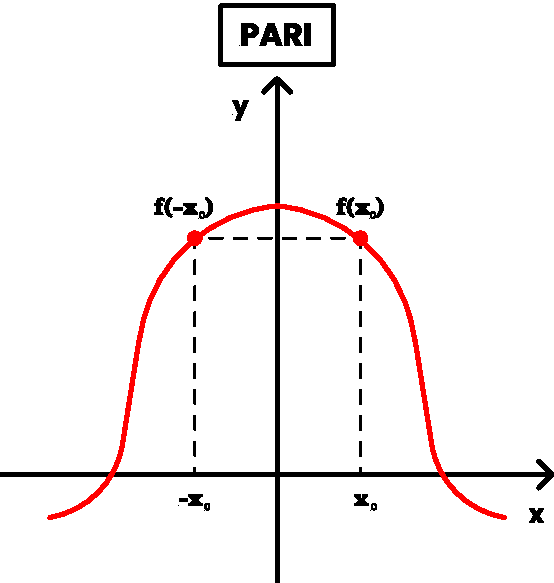
\includegraphics[width=7cm]{./images/evenFunctions.pdf}\hfill
    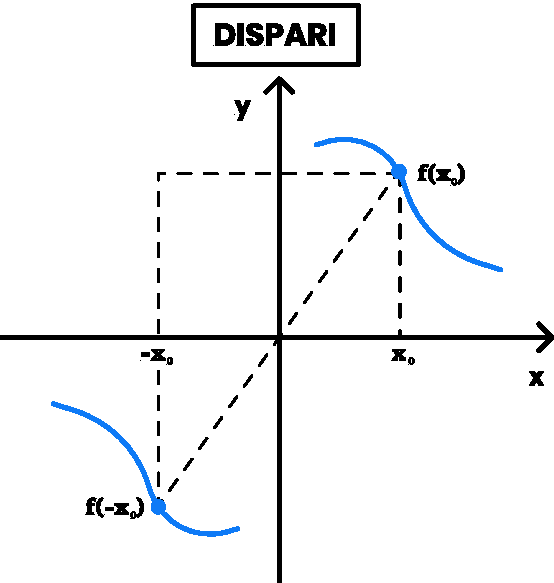
\includegraphics[width=7cm]{./images/oddFunctions.pdf}
\end{figure}

\noindent\textbf{Proposizione:} Sia $a > 0$, consideriamo quindi $A = (-a, a) - \{0\}$. Sia inoltre $f: A \xrightarrow{} \mathbb{R}$ una funzione pari. Supponiamo che:
\begin{equation*}
    \lim_{ \underset{\scriptstyle (x \to 0^+)}{x \to 0^-}} f(x) = l \in \widetilde{\mathbb{R}} \implies \lim_{ \underset{\scriptstyle (x \to 0^-)}{x \to 0^+}} f(x) = l
\end{equation*}

\noindent Dimostriamo questa proposizione. Supponiamo di conoscere:
\begin{equation*}
    l = \lim_{\underset{\scriptstyle (x \to 0^+)}{x \to 0^-}} f(x)
\end{equation*}

\noindent Utilizziamo ora il teorema dei limiti per sostituzione, attraverso la funzione:
\begin{equation*}
    u: A \xrightarrow{} \mathbb{R} \quad x \longmapsto -x \implies \lim_{\underset{\scriptstyle (x \to 0^+)}{x \to 0^-}} u(x) = 0^+ \ (0^-)
\end{equation*}

\noindent Otteniamo quindi: 
\begin{equation*}
    l = \lim_{\underset{\scriptstyle (x \to 0^+)}{x \to 0^-}} f(x) = \lim_{\underset{\scriptstyle (u \to 0^-)}{u \to 0^+}} f(-u)
\end{equation*}

\noindent Dato che la funzione $f$ è pari, allora possiamo scrivere:
\begin{equation*}
    l = \lim_{\underset{\scriptstyle (x \to 0^+)}{x \to 0^-}} f(x) = \lim_{\underset{\scriptstyle (u \to 0^-)}{u \to 0^+}} f(-u) = \lim_{\underset{\scriptstyle (u \to 0^-)}{u \to 0^+}} f(u)
\end{equation*}

\noindent Abbiamo quindi dimostrato che il limite destro e il limite sinistro sono uguali per funzioni pari.\\

\noindent\textbf{Proposizione:} Sia $a > 0$ e $A = (-a, a) - \{0\}$. Sia inoltre $f: A \subset \mathbb{R}$ una funzione dispari. Allora:
\begin{itemize}
    \item se $\lim_{\underset{\scriptstyle (x \to 0^+)}{x \to 0^-}} f(x) = l \in \mathbb{R} \implies \lim_{\underset{\scriptstyle (x \to 0^-)}{x \to 0^+}} f(x) = -l \in \mathbb{R}$;
    \item se $\lim_{\underset{\scriptstyle (x \to 0^+)}{x \to 0^-}} f(x) = +\infty \implies \lim_{\underset{\scriptstyle (x \to 0^-)}{x \to 0^+}} f(x) = -\infty$;
    \item se $\lim_{\underset{\scriptstyle (x \to 0^+)}{x \to 0^-}} f(x) = -\infty \implies \lim_{\underset{\scriptstyle (x \to 0^-)}{x \to 0^+}} f(x) = +\infty$;
\end{itemize}

\noindent Procediamo dimostrando la proposizione qui sopra. Innanzitutto, sfruttiamo il teorema dei limiti per sostituzione come al solito con $u(x) = -x$:
\begin{equation*}
    \lim_{\underset{\scriptstyle (x \to 0^-)}{x \to 0^+}} f(x) = \lim_{\underset{\scriptstyle (u \to 0^+)}{u \to 0^-}} f(-u)
\end{equation*}

\noindent Ora dato che stiamo valutando una funzione dispari, si ha che:
\begin{equation*}
    \lim_{\underset{\scriptstyle (x \to 0^-)}{x \to 0^+}} f(x) = \lim_{\underset{\scriptstyle (u \to 0^+)}{u \to 0^-}} f(-u) = \lim_{\underset{\scriptstyle (u \to 0^+)}{u \to 0^-}} (-f(-u)) = - \lim_{\underset{\scriptstyle (u \to 0^+)}{u \to 0^-}} f(-u)
\end{equation*}

\noindent Ciò significa che il valore del limite sinistro della funzione sarà uguale al valore del limite destro di quella funzione, ma cambiato di segno.\\

\noindent\textbf{ES.} Sia $f$ pari (o dispari) con $D_f$ non limitato e simmetrico rispetto a 0. Allora detti:
\begin{equation*}
    \lim_{x \to +\infty} \frac{f(x)}{x} = m_1 \in \mathbb{R} \qquad \lim_{x \to -\infty} \frac{f(x)}{x} = m_2 \in \mathbb{R}
\end{equation*}
\begin{equation*}
    \lim_{x \to +\infty} (f(x) - m_1x) = n_1 \in \mathbb{R} \qquad \lim_{x \to -\infty} (f(x) - m_1x) = n_2 \in \mathbb{R}
\end{equation*}

\noindent Che relazione esiste tra $m_1$ e $m_2$? E tra $n_1$ e $n_2$?\\
Se la funzione è pari, allora:
\begin{equation*}
    m_2 = \lim_{x \to -\infty} \frac{f(x)}{x}
\end{equation*}

\noindent e usando la solita sostituzione $u = -x$:
\begin{equation*}
    m_2 = \lim_{x \to -\infty} \frac{f(x)}{x} = \lim_{u \to +\infty} \frac{f(-u)}{-u}
\end{equation*}

\noindent Ora dato che la funzione è pari, si ha che:
\begin{equation*}
    m_2 = \lim_{x \to -\infty} \frac{f(x)}{x} = \lim_{u \to +\infty} \frac{f(-u)}{-u} = \lim_{u \to +\infty} \frac{f(u)}{-u} = -\lim_{u \to +\infty} \frac{f(u)}{u} = -m_1 \implies m_2 = -m_1
\end{equation*}

\noindent Mentre considerando $n_1$ e $n_2$, basta sapere dalla dimostrazione precedente che $m_2 = -m_1$ e basta applicare la sostituzione $u = -x$:
\begin{equation*}
    n_2 = \lim_{x \to -\infty} (f(x) - m_2x) = \lim_{x \to -\infty} (f(x) + m_1x) = \lim_{u \to +\infty} (f(-u) + m_1(-u)) = \lim_{u \to +\infty} (f(u) - m_1u) = n_1
\end{equation*}

\noindent Consideriamo ora il caso in cui la funzione sia dispari. Allora:
\begin{equation*}
    m_2 = \lim_{x \to -\infty} \frac{f(x)}{x} = \lim_{u \to +\infty} \frac{f(-u)}{-u} = \lim_{u \to +\infty} \frac{-f(u)}{-u} = \lim_{u \to +\infty} \frac{f(u)}{u} = m_1 \implies m_2 = m_1
\end{equation*}

\noindent Mentre considerando $n_1$ e $n_2$, basta sapere dalla dimostrazione precedente che $m_2 = m_1$ e basta applicare la sostituzione $u = -x$:
\begin{equation*}
    n_2 = \lim_{x \to -\infty} (f(x) - m_2x) = \lim_{x \to -\infty} (f(x) - m_1x) = \lim_{u \to +\infty} (f(-u) - m_1(-u)) = \lim_{u \to +\infty} (-f(u) + m_1u)
\end{equation*}
\begin{equation*}
    = - \lim_{u \to +\infty} (f(u) - m_1u) = -n_1 \implies n_2 = -n_1
\end{equation*}

\noindent\textbf{NB!} Nel testo dell'esercizio qui sopra è stato specificato che la funzione dovesse essere pari o dispari e che il dominio fosse limitato, ma quando una funzione è pari o dispari, allora ci basta sapere che il dominio è o superiormente o inferiormente limitato per poter concludere che esso è limitato (essendo simmetrico).\\

\noindent Dopo aver fornito alcuni strumenti utili, ritorniamo a dimostrare alcuni limiti notevoli.\\
Dimostriamo ora il primo (\ref{eq:limnot1}) e il secondo (\ref{eq:limnot2}) limite notevole. Per prima cosa dobbiamo verificare che $+\infty$ e $-\infty$ siano dei punti di accumulazione per il dominio di queste funzioni, altrimenti non avrebbe senso parlare di limite.\\

\noindent\textbf{NB!} $f(x)^{g(x)} \vcentcolon= e^{(\log(f(x))g(x)}$ con $f(x) > 0$.\\

\noindent Per la proprietà qui sopra enunciata, possiamo dire che:
\begin{equation*}
    \left(1 + \frac{1}{x}\right)^x = e^{x\log(1 + \frac{1}{x})}
\end{equation*}

\noindent Dato che stiamo parlando di un esponenziale, le uniche condizioni di esistenza possono trovarsi nel suo esponente. In particolare, abbiamo le seguenti condizioni di esistenza:
\begin{equation*}
    \begin{cases}
        x \in \mathbb{R}\\
        x \neq 0 \\
        1 + \frac{1}{x} > 0
    \end{cases}
    \iff
    \begin{cases}
        x \neq 0 \\
        \dfrac{x + 1}{x} > 0
    \end{cases}
\end{equation*}

\noindent Dividiamo ora il sistema e risolviamolo:
\begin{equation*}
    \begin{cases}
        x \neq 0 \\
        x > -1 \\
        x > 0
    \end{cases}
    \implies (0, +\infty) \qquad \qquad
    \begin{cases}
        x \neq 0 \\
        x < -1 \\
        x < 0
    \end{cases}
    \implies (-\infty, -1)
\end{equation*}

\noindent Il dominio risulta essere quindi $D_f = (-\infty, -1) \cup (0, +\infty)$. Non essendo simmetrico, possiamo già intuire che la funzione non è né pari, né dispari. Da com'è fatto il dominio capiamo che $+\infty$ e $-\infty$ sono punti di accumulazione per esso, per cui ha senso parlare di limiti.\\
Partiamo calcolando i limiti per $x \to +\infty$. Consideriamo quindi $x > 1$, allora per la proprietà della parte intera si ha che:
\begin{equation*}
    0 < 1 \leq \lfloor x \rfloor \leq x < \lfloor x \rfloor + 1
\end{equation*}

\noindent Essendo tutti valori positivi, possiamo effettuare il reciproco, che cambierà il verso di tutte le disequazioni. Otteniamo quindi:
\begin{equation*}
    \frac{1}{\lfloor x \rfloor} \geq \frac{1}{x} > \frac{1}{\lfloor x \rfloor + 1}
\end{equation*}

\noindent A questo punto, dato che la nostra funzione ha come argomento $(1 + \frac{1}{x})$, aggiungiamo $1$ da tutte le parti:
\begin{equation*}
      1 + \frac{1}{\lfloor x \rfloor} \geq 1 + \frac{1}{x} > 1 + \frac{1}{\lfloor x \rfloor + 1} > 1
\end{equation*}

\noindent Eleviamo quindi alla $x$:
\begin{equation*}
      \left(1 + \frac{1}{\lfloor x \rfloor}\right)^x \geq \left(1 + \frac{1}{x}\right)^x > \left(1 + \frac{1}{\lfloor x \rfloor + 1}\right)^x
\end{equation*}

\noindent Dato che agli estremi vogliamo solo numeri naturali, mentre $x \in \mathbb{R}$, allora possiamo sfruttare la proprietà della parte intera per dire che:
\begin{equation*}
     \left(1 + \frac{1}{\lfloor x \rfloor}\right)^{\lfloor x \rfloor + 1} > \left(1 + \frac{1}{\lfloor x \rfloor}\right)^x \qquad \left(1 + \frac{1}{\lfloor x \rfloor + 1}\right)^x \geq \left(1 + \frac{1}{\lfloor x \rfloor + 1}\right)^{\lfloor x \rfloor}
\end{equation*}

\noindent Quindi:
\begin{equation*}
      \left(1 + \frac{1}{\lfloor x \rfloor + 1}\right)^{\lfloor x \rfloor} \leq \left(1 + \frac{1}{x}\right)^x < \left(1 + \frac{1}{\lfloor x \rfloor}\right)^{\lfloor x \rfloor + 1}
\end{equation*}

\noindent Notiamo ora che sia il termine più a sinistra, che il termine più a destra assomigliano molto alla successione: $\lim_{n \to +\infty} (1 + \frac{1}{n})^n = e$. Cerchiamo quindi di ricondurci ad esso:
\begin{equation*}
    \lim_{x \to +\infty} \left(1 + \frac{1}{\lfloor x \rfloor + 1}\right)^{\lfloor x \rfloor} = \lim_{k \to +\infty} \left(1 + \frac{1}{k + 1}\right)^k
\end{equation*}

\noindent Aggiungiamo ora un $1 + \frac{1}{k + 1}$:
\begin{equation*}
    \lim_{x \to +\infty} \left(1 + \frac{1}{\lfloor x \rfloor + 1}\right)^{\lfloor x \rfloor} = \lim_{k \to +\infty} \left(1 + \frac{1}{k + 1}\right)^k = \lim_{k \to +\infty} \frac{\left(1 + \frac{1}{k + 1}\right)^{k + 1}}{\left(1 + \frac{1}{k + 1}\right)}
\end{equation*}

\noindent Ora notiamo che, per $k \to +\infty$, il denominatore tende a $1$, mentre il numeratore è proprio il limite di successione notevole che conosciamo:
\begin{equation*}
    \implies \lim_{x \to +\infty} \left(1 + \frac{1}{\lfloor x \rfloor + 1}\right)^{\lfloor x \rfloor} = e
\end{equation*}

\noindent Prendiamo ora il secondo termine della proprietà della parte intera:
\begin{equation*}
    \lim_{x \to +\infty} \left(1 + \frac{1}{\lfloor x \rfloor}\right)^{\lfloor x \rfloor + 1} = \lim_{k \to +\infty} \left(1 + \frac{1}{k}\right)^{k + 1} = \lim_{k \to +\infty} \left(1 + \frac{1}{k}\right)^k \left(1 + \frac{1}{k}\right)
\end{equation*}

\noindent Ancora una volta $\lim_{k \to +\infty} \left(1 + \frac{1}{k}\right) = 1$ e $\lim_{k \to +\infty} \left(1 + \frac{1}{k}\right)^k = e$, quindi per il teorema del limite del prodotto $\lim_{k \to +\infty} \left(1 + \frac{1}{k}\right) \left(1 + \frac{1}{k}\right) = e$.
\begin{equation*}
    \implies \lim_{x \to +\infty} \left(1 + \frac{1}{\lfloor x \rfloor}\right)^{\lfloor x \rfloor + 1} = e
\end{equation*}

\noindent Infine, dato che sia entrambi i termini "alle estremità" della parte intera tendono a $e$ per $x \to +\infty$, allora per il teorema dei carabinieri si ha che:
\begin{equation*}
    \lim_{x \to +\infty} \left(1 + \frac{1}{x}\right)^x = e
\end{equation*}

\noindent Consideriamo ora il caso di $x < 0$ e quindi calcoliamo i limiti per $x \to -\infty$. Chiamiamo $f(x) = (1 + \frac{1}{x})^x$, allora, effettuando la sostituzione $t = -x$, si ha che:
\begin{equation*}
    \lim_{x \to -\infty} \left(1 + \frac{1}{x}\right)^x = \lim_{t \to +\infty} f(-t)
\end{equation*}

\noindent Ma se calcoliamo $f(-t)$:
\begin{equation*}
    f(-t) = \left(1 - \frac{1}{t}\right)^{-t} = \left(\frac{t - 1}{t}\right)^{-t} = \left(\frac{t}{t - 1}\right)^t = \left(1 + \frac{1}{t - 1}\right)^t = \left(1 + \frac{1}{t - 1}\right)^{t-1}\left(1 + \frac{1}{t - 1}\right)
\end{equation*}
\begin{equation*}
    \implies \lim_{t \to +\infty} \left(1 + \frac{1}{t - 1}\right)^{t-1}\left(1 + \frac{1}{t - 1}\right) = e = \lim_{x \to -\infty} \left(1 + \frac{1}{x}\right)^x
\end{equation*}

\noindent Dimostriamo ora il nono limite notevole (\ref{eq:limnot9}) con $x \in \mathbb{R}$. Partiamo dal caso in cui $x = 0$, allora semplicemente si ha che:
\begin{equation*}
    \lim_{n \to +\infty} \left(1 + \frac{0}{n}\right)^n =  \lim_{n \to +\infty} 1^n = 1 = e^0
\end{equation*}

\noindent Prendiamo ora il caso in cui $x > 0$. Utilizzando la sostituzione $t = \frac{n}{x}$, si ha che:
\begin{equation*}
    \lim_{n \to +\infty} \left(1 + \frac{x}{n}\right)^n = \lim_{t \to +\infty} \left(1 + \frac{1}{t}\right)^{tx} = \left[\lim_{t \to +\infty} \left(1 + \frac{1}{t}\right)^t\right]^x = e^x
\end{equation*}

\noindent (abbiamo spostato la "$x$" al di fuori dal limite, tanto il suo valore non dipende dal limite stesso). Consideriamo ora il caso $x < 0$ e anche qui applichiamo la sostituzione $t = -\frac{n}{x}$, perché prendiamo $x$ direttamente con il segno (dato che è presente un "-", se $n \to +\infty$, allora $t \to -\infty$. Non importa che sia $+\infty$, tanto considerando la sostituzione fatta, non ci troviamo più nei naturali, ma nei reali. Per cui anche $-\infty$ è un punto di accumulazione):
\begin{equation*}
    \lim_{n \to +\infty} \left(1 - \frac{x}{n}\right)^n = \lim_{t \to -\infty} \left(1 + \frac{1}{t}\right)^{-tx} = \left[\lim_{t \to -\infty} \left(1 + \frac{1}{t}\right)^t\right]^{-x} = e^{-x}
\end{equation*}

\noindent (è giusto che esca $-x$ perché abbiamo preso $x$ con il segno. Se invece avessimo effettuato tutti i conti considerando semplicemente $x < 0$, allora sarebbe uscito $e^x$). Effettuando gli stessi passaggi e le stesse sostituzioni, è possibile dimostrare anche il decimo (\ref{eq:limnot10}) e l'undicesimo (\ref{eq:limnot11}) limite notevole (ovviamente in questi due limiti, bisogna considerare i casi $a > 0$, $a = 0$ e $a < 0$; non cosa succede ad $x$).\\

\noindent Dimostriamo ora il terzo limite notevole (\ref{eq:limnot3}). Sia $x > 0$, allora applichiamo la sostituzione $t = \frac{1}{x}$. Quindi se $x \to 0^+$, abbiamo che:
\begin{equation*}
    \lim_{x \to 0^+} (1 + x)^\frac{1}{x} = \lim_{t \to +\infty} \left(1 + \frac{1}{t}\right)^t = e
\end{equation*}

\noindent mentre se $x \to 0^-$, abbiamo che
\begin{equation*}
    \lim_{x \to 0^-} (1 + x)^\frac{1}{x} = \lim_{t \to -\infty} \left(1 + \frac{1}{t}\right)^t = e
\end{equation*}

\noindent Dimostriamo ora il settimo limite notevole (\ref{eq:limnot7}). Innanzitutto, calcoliamo il dominio: 
\begin{equation*}
    D_f = 
    \begin{cases}
        (1 + x)^a \iff x > -1 \\
        x \neq 0
    \end{cases}
    \implies (-1, 0) \cup (0, +\infty)
\end{equation*}

\noindent La prima condizione è dovuta al fatto che la base di un esponenziale deve essere maggiore di $0$. Notiamo inoltre dal dominio che $x_0 = 0$ è punto di accumulazione per esso. Ora:
\begin{itemize}
    \item se $a = 0$, dato che $(1 + x)^a \vcentcolon = e^{a\log(1 + x)} = 1 \qquad \forall x \in \mathbb{R}$, allora il numeratore è pari a $0$ e quindi: $$\lim_{x \to 0} \frac{(1 + x)^a - 1}{x} = \lim_{x \to 0} 0 = 0 = a$$
    \item se $a \neq 0$ e $x > -1$, allora sappiamo che $\lim_{x \to 0} \log(1 + x) = 0 \implies (1 + x)^a = e^{a\log(1 + x)} = 1$. Mentre prima il numeratore era pari a $0$, qui tende a $0$, come il denominatore. Ci troviamo quindi in un caso di indeterminazione. Poniamo allora $(1 + x)^a - 1 = t \iff (t + 1) = (1 + x)^a \implies a\log(1 + x) = \log(t + 1)$. Quindi: $$\lim_{x \to 0} \frac{(1 + x)^a - 1}{x} = \lim_{x \to 0} \frac{(1 + x)^a - 1}{\log(1 + x)} \cdot \frac{\log(1 + x)}{x} = \lim_{t \to 0} \frac{t}{\frac{1}{a} \log(1 + t)} = a\lim_{t \to 0}\frac{t}{\log(1 + t)} = a$$
\end{itemize}

\subsection{Esercizi su limiti e simmetrie}
\subsubsection{Esercizio 14}
Sia $f(x) \in [0, |x|] \qquad \forall x \neq 0, \ con \ x \in D_f$. Allora dimostriamo che $\lim_{x \to 0} f(x) = 0$.\\
È possibile risolvere l'esercizio utilizzando due metodologie differenti. Sapendo che:
\begin{equation*}
    0 \leq f(x) \leq |x|
\end{equation*}

\noindent Ora dato che $\lim_{x \to 0} 0 = 0$ e che $\lim_{x \to 0} |x| = 0$, allora per il teorema dei carabinieri $\lim_{x \to 0} f(x) = 0$.\\
Altrimenti è possibile applicare la definizione di limite. Sia quindi $x \neq 0$ e sia $\varepsilon > 0$. Consideriamo allora $|f(x) - 0| = |f(x)|$. Dato che $f(x) \geq 0$ per ipotesi, allora $|f(x)| = f(x)$. Sempre per ipotesi sappiamo che $f(x) \leq |x| = |x - 0|$. Poniamo ora $\delta_\varepsilon = \varepsilon$ e consideriamo $0 < |x| < \delta_\varepsilon$. Quindi:
\begin{equation*}
    \forall \varepsilon > 0, \exists \delta_\varepsilon > 0 \ (\delta_\varepsilon = \varepsilon) \ tale \ che \ |f(x) - 0| < \delta_\varepsilon \qquad \forall x \in D_f, \ 0 < |x| < \delta_\varepsilon \implies \lim_{x \to 0} f(x) = 0
\end{equation*}

\subsubsection{Esercizio 15}
Mostrare che $f(x) \vcentcolon = x^n$ è pari $\iff n$ è pari e che $f(x) \vcentcolon = x^n$ è dispari $\iff n$ è dispari. \\

\noindent Mostriamo, innanzitutto, l'implicazione ($\Rightarrow$). Sia $x \neq 0$, dato che $f(-x) = (-x)^n = (-1)^n (x)^n$ e $f(x) = x^n$, allora, se $f(x)$ è pari si ha che:
\begin{equation*}
    (-1)^n (x)^n = (x)^n \implies (-1)^n = 1 \implies n \ pari
\end{equation*}

\noindent Dimostriamo ora la controimplicazione ($\Leftarrow$). Se $n$ è pari, allora possiamo riscriverlo come $n = 2k$ e quindi:
\begin{equation*}
    f(-x) = (-x)^{2k} = (-1)^{2k} (x)^{2k} = x^{2k} = f(x) \implies f(x) \ pari
\end{equation*}

\noindent Mostriamo, innanzitutto, l'implicazione ($\Rightarrow$). Sia $x \neq 0$, dato che $f(-x) = (-x)^n = (-1)^n (x)^n$ e $-f(x) = -(x^n)$, allora, se $f(x)$ è dispari si ha che:
\begin{equation*}
    (-1)^n (x)^n = -(x)^n \implies (-1)^n = -1 \implies n \ dispari
\end{equation*}

\noindent Dimostriamo ora la controimplicazione ($\Leftarrow$). Se $n$ è dispari, allora possiamo riscriverlo come $n = 2k + 1$ e quindi:
\begin{equation*}
    f(-x) = (-x)^{2k + 1} = (-1)^{2k + 1} (x)^{2k + 1} = -x^{2k + 1} = -f(x) \implies f(x) \ dispari
\end{equation*}

\subsubsection{Esercizio 16}
\textbf{Punto 1.} Siano $f, g$ pari, allora mostrare che $f + g$, $f - g$ e $f \cdot g$ sono anch'esse pari.
\begin{equation*}
    (f \pm g)(-x) = f(-x) \pm g(-x) = f(x) \pm g(x) = (f \pm g)(x)
\end{equation*}
\begin{equation*}
    (f \cdot g)(-x) = f(-x) \cdot g(-x) = f(x) \cdot g(x) = (f \cdot g)(x)
\end{equation*}

\noindent\textbf{Punto 2.} Siano $f, g$ dispari, allora mostrare che $f + g$ e $f - g$ sono dispari, mentre $f \cdot g$ è pari.
\begin{equation*}
    (f \pm g)(-x) = f(-x) \pm g(-x) = -f(x) \mp g(x) = -(f(x) \pm g(x)) = - (f \pm g)(x)
\end{equation*}
\begin{equation*}
    (f \cdot g)(-x) = f(-x) \cdot g(-x) = -f(x) \cdot (-g(x)) = (f \cdot g)(x)
\end{equation*}

\noindent\textbf{Punto 3.} Sia $f$ pari e $g$ dispari, allora mostrare che $f \cdot g$ è dispari.
\begin{equation*}
    (f \cdot g)(-x) = f(-x) \cdot g(-x) = f(x) \cdot (-g(x)) = - (f \cdot g)(x)
\end{equation*}

\noindent\textbf{NB!} Non abbiamo calcolato le simmetrie di $(f \pm g)(x)$ perché quando $f$ è pari e $g$ è dispari, o viceversa, in queste funzioni può accadere di tutto. Ad esempio, siano $f(x) = x^2$ (è una funzione pari) e $g(x) = x$ (è una funzione dispari). Sia quindi $h(x) = (f + g)(x) = x^2 + x = x(x + 1)$. Notiamo come $h(x)$ si annulli in $-1$ ($h(-1) = 0$), ma $h(1) \neq 0$ (per la precisione, $h(1) = 2$). Quindi $h(x)$ non è né pari, né dispari. Otteniamo lo stesso identico risultato (ma invertito), se consideriamo $h(x) = (f - g)(x)$.\\

\noindent\textbf{Punto 4.} Siano $f, g$ pari, allora mostrare che $\frac{f}{g}$ è pari. \\
\noindent\textbf{Punto 5.} Siano $f, g$ dispari, allora mostrare che $\frac{f}{g}$ è pari.\\
\noindent\textbf{Punto 6.} Sia $f$ pari e $g$ dispari, allora mostrare che $\frac{f}{g}$ è dispari.\\
In generale, per risolvere questi punti basta osservare che se $g(x) \neq 0 \qquad \forall x \in \mathbb{R}$, allora:
\begin{itemize}
    \item se $g$ è pari $\implies h = \frac{1}{g}$ è pari, dato che: $$h(-x) = \frac{1}{g(-x)} = \frac{1}{g(x)} = h(x)$$
    \item se $g$ è dispari $\implies h = \frac{1}{g}$ è dispari, dato: che $$h(-x) = \frac{1}{g(-x)} = -\frac{1}{g(x)} = -h(x)$$
\end{itemize}

\noindent Successivamente, si procede utilizzando le considerazioni fatte nelle applicazioni prodotto dei punti precedenti.

\subsubsection{Esercizio 17}
Determinare $a \in \mathbb{R}$ tale che:
\begin{equation*}
    \lim_{x \to +\infty} \left(\frac{x^3 + ax^2 + x}{x^2 - ax + 1} - (x + 2)\right) = 0
\end{equation*}

\noindent Innanzitutto, determiniamo il dominio. Dobbiamo stare attenti a quando il denominatore si annulla, ovvero quando $x^2 - ax + 1 = 0$. Ciò avviene quando:
\begin{equation*}
    x = x_1 = \frac{a + \sqrt{a^2 - 4}}{2} \quad oppure \quad x = x_2 = \frac{a - \sqrt{a^2 - 4}}{2}
\end{equation*}

\noindent e vale solo quando l'argomento della radice è maggiore o uguale a zero ($a^2 - 4 \geq 0$). \\
Quindi per $a \in (-2, 2)$ il denominatore non si annulla e quindi $D_f = \mathbb{R}$. Se invece $a = 2$, allora al denominatore avremmo che $x^2 - 2x + 1 = (x - 1)^2$ e quindi esso si annulla per $x_{1, 2} = 1$. Ciò significa che in questo caso $D_f = \mathbb{R} - \{1\}$. Allo stesso modo, se $a = -2$, allora al denominatore avremmo che $x^2 + 2x + 1 = (x + 1)^2$ e quindi esso si annulla per $x_{1, 2} = -1$. Ciò significa che in questo caso $D_f = \mathbb{R} - \{-1\}$. Infine, se $a \in (-\infty, -2) \cup (2, +\infty)$, allora il denominatore si annulla in $x_1$ e $x_2$ scritti qui sopra, quindi $D_f = \mathbb{R} - \{x_1, x_2\}$.\\
In ogni caso, notiamo che $+\infty$ è punto di accumulazione per $D_f \ \forall a \in \mathbb{R}$. Possiamo quindi procedere a risolvere il limite. Innanzitutto, concentriamoci sul suo argomento e svolgiamo il denominatore comune:
\begin{align*}
    \frac{x^3 + ax^2 + x}{x^2 - ax + 1} - (x + 2) &= \frac{x^3 + ax^2 + x - (x + 2)(x^2 - ax + 1)}{x^2 - ax + 1} \\
    &= \frac{x^3 + ax^2 + x - x^3 + ax^2 - x - 2x^2 + 2ax - 2}{x^2 - ax + 1} \\
    &= \frac{2x^2(a - 1) + 2ax - 2}{x^2 - ax + 1}
\end{align*}

\noindent Riscriviamo ora il limite, raccogliendo $x^2$ sia nel numeratore che nel denominatore. Notiamo poi che molti dei termini presenti tendono a $0$ quando $x \to +\infty$:
\begin{equation*}
    \lim_{x \to +\infty} \frac{2x^2(a - 1) + 2ax - 2}{x^2 - ax + 1} = \lim_{x \to +\infty} \frac{x^2\left(2(a - 1) + \frac{2a}{x} - \frac{2}{x^2}\right)}{x^2\left(1 - \frac{a}{x} + \frac{1}{x^2}\right)} = 2(a - 1) = 2a - 2
\end{equation*}

\noindent Dato che l'esercizio chiedeva di trovare il valore di $a$ per cui il limite fosse uguale a $0$, non ci resta che risolvere $2a - 2 = 0$, che è chiaramente $a = 1$.

\subsubsection{Esercizio 18}
Sia $f(x) = \lfloor x \rfloor \sin(\frac{1}{x^2})$, esiste $\lim_{x \to 0} f(x)$?\\

\noindent Dividiamo il caso "limite destro" dal caso "limite sinistro". Se $x \in (0, 1)$, allora $\lfloor x \rfloor = 0$ e quindi $f(x) = 0$. Ciò significa che $\lim_{x \to 0^+} f(x) = 0$.\\
Se invece $x \in (-1, 0)$, si ha che $\lfloor x \rfloor = 1$, quindi la funzione diventa $f(x) = -\sin(\frac{1}{x^2})$. Utilizziamo ora il teorema ponte. Prendiamo quindi:
\begin{equation*}
    a_n = - \frac{1}{\sqrt{\frac{\pi}{2} + 2\pi n}} \ con \ n \in \mathbb{N}, n \geq 1 \implies \frac{1}{a_n^2} = \frac{\pi}{2} + 2\pi n
\end{equation*}
\begin{equation*}
    b_n = - \frac{1}{\sqrt{-\frac{\pi}{2} + 2\pi n}} \ con \ n \in \mathbb{N}, n \geq 1 \implies \frac{1}{b_n^2} = - \frac{\pi}{2} + 2\pi n
\end{equation*}

\noindent (non stiamo commettendo un errore nel denominatore di $b_n$ perché $2 \pi n$ è sicuramente maggiore di $\frac{\pi}{2}$, per cui la loro differenza non è negativa). Dato che $\lim_{n \to +\infty} a_n = \lim_{n \to +\infty} b_n = 0 = x_0$, allora se effettivamente esistesse il limite di $-\sin(\frac{1}{x^2})$, si avrebbe che $\lim_{n \to +\infty} -\sin(a_n) = \lim_{n \to +\infty} -\sin(b_n) = \lim_{x \to 0} -\sin(\frac{1}{x^2})$. Dato però che:
\begin{equation*}
    \sin\left(\frac{1}{a_n^2}\right) = \sin\left(\frac{\pi}{2} + 2\pi n\right) = 1 \qquad \sin\left(\frac{1}{b_n^2}\right) = \sin\left(-\frac{\pi}{2} + 2\pi n\right) = -1
\end{equation*}

\noindent Allora il limite non esiste, perché se esistesse dovrebbe avere lo stesso valore in tutte le successioni.

\subsubsection{Esercizio 19}
Sia $f: \mathbb{R} \xrightarrow{} \mathbb{R}$. Dimostriamo che $f$ è una funzione affine $\iff f(x + y) = f(x) + (f(1) - f(0))y \qquad \forall x, y \in \mathbb{R}$.\\

\noindent\textbf{NB!} Una funzione si dice \textbf{affine} quando è del tipo $f(x) = ax + b \qquad \forall a, b \in \mathbb{R}$.\\

\noindent Dimostriamo, innanzitutto, l'implicazione ($\Leftarrow$). Per definizione sappiamo che $f(x) = ax + b$, quindi $f(1) = a + b$, $f(0) = b$ e $f(1) - f(0) = a$. Ora è facile notare che:
\begin{equation*}
    f(x + y) = a(x + y) = b = ax + b + ay = f(x) + (f(1) - f(0))y
\end{equation*}

\noindent Dimostriamo ora la controimplicazione ($\Rightarrow$). Consideriamo il caso $x = t$ e $y = 1$, allora per ipotesi:
\begin{equation*}
    f(t + 1) = f(t) + (f(1) - f(0))
\end{equation*}

\noindent Consideriamo ora il caso $x = 1$ e $y = t$, allora per ipotesi:
\begin{equation*}
    f(1 + t) = f(1) + (f(1) - f(0))t
\end{equation*}

\noindent Notiamo però che i due casi descrivono la stessa funzione per cui:
\begin{equation*}
    f(t) + (f(1) - f(0)) = f(1) + (f(1) - f(0))t \implies f(t) = (f(1) - f(0))t + f(0)
\end{equation*}

\noindent Sia ora $a = f(1) - f(0)$ e $b = f(0)$, allora si ottiene che $f(t) = at + b$.

\subsubsection{Esercizio 20}
Sia $f: \mathbb{R} \xrightarrow{} \mathbb{R}$ una funzione affine.\\
$\forall y \in \mathbb{R}$, sia:
\begin{equation*}
    g(y) \vcentcolon = \lim_{x \to y} \frac{f(x) - f(y)}{x - y}
\end{equation*}

\noindent allora $g(y)$ è una funzione costante.\\

\noindent Dato che $f$ affine significa che $\exists a, b \in \mathbb{R} : f(x) = ax + b \qquad \forall x \in \mathbb{R} \ con \ a \neq 0$. Allora, fissato $y \in \mathbb{R}$, per $x \neq y$ si ha che:
\begin{equation*}
    \frac{f(x) - f(y)}{x - y} = \frac{ax + b - ay - b}{x - y} = \frac{a(x - y)}{x - y} = a \qquad \forall y \in \mathbb{R}, \forall x \neq y
\end{equation*}

\noindent Pertanto si ottiene una funzione costante: 
\begin{equation*}
    \lim_{x \to y} \frac{f(x) - f(y)}{x - y} = a \qquad \forall y \in \mathbb{R}
\end{equation*}

\subsubsection{Esercizio 21}
Sia $f: \mathbb{R} \xrightarrow{} \mathbb{R}$ una funzione quadratica $f(x) = ax^2 + bx + c$ con $a, b, c \in \mathbb{R}$.\\
$\forall y \in \mathbb{R}$, sia:
\begin{equation*}
    g(y) \vcentcolon = \lim_{x \to y} \frac{f(x) - f(y)}{x - y}
\end{equation*}

\noindent allora $g(y)$ è una funzione affine.\\

\noindent La dimostrazione è abbastanza semplice:
\begin{align*}
    \lim_{x \to y} \frac{f(x) - f(y)}{x - y} &= \lim_{x \to y} \frac{ax^2 + bx + c - ay^2 - by - c}{x - y} \\
    &= \lim_{x \to y} \frac{a(x^2 - y^2) + b(x - y)}{x - y} \\
    &= \lim_{x \to y} \frac{(x - y)[a(x + y) + b]}{x - y} \\
    &= \lim_{x \to y} (ax + ay + b) = 2ay + b
\end{align*}

\noindent\textbf{Proposizione:} Sia $x \in (0, \frac{\pi}{2})$. Allora $0 < \sin(x) < x < \tan(x)$. Inoltre, si ha che $|\sin(x)| \leq |x| \qquad \forall x \in \mathbb{R}$.\\

\noindent Partiamo dimostrando che se $x \in (0, \frac{\pi}{2})$ allora $0 < \sin(x) < x < \tan(x)$. Aiutiamoci con un disegno a capire i conti che svolgeremo.

\begin{wrapfigure}{r}{0.5\textwidth}
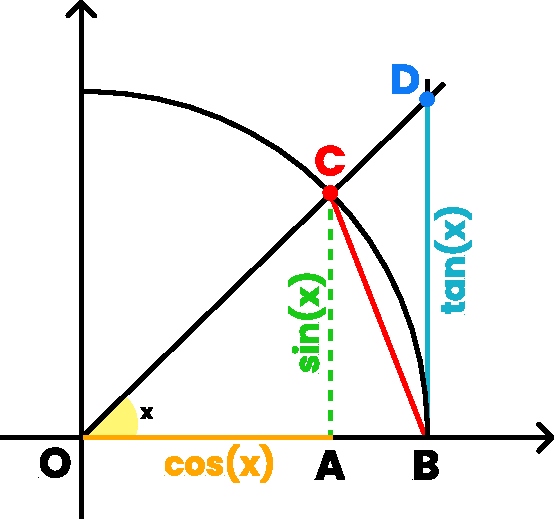
\includegraphics[width=0.9\linewidth]{./images/proposition.pdf}
\end{wrapfigure}

\noindent Chiamiamo quindi $\overline{AC} = \sin(x)$, $\overline{BD} = \tan(x)$ e $S$ il settore circolare. Notiamo subito che il settore circolare $S$ contiene il triangolo $OCB$, in simboli: $T_{OCB} \subsetneq S$.\\
Sappiamo poi che $Area(T_{OCB}) = \frac{\sin(x) \cdot \overline{OB}}{2} = \frac{\sin(x)}{2}$, essendo che $\overline{OB} = 1$, dato che il cerchio che stiamo considerando ha raggio $1$. Mentre, sapendo che l'area di un settore circolare è pari a $A = \frac{r^2 \beta}{2}$, ma qui $r = 1$ e $\beta = x$, allora $Area(S) = \frac{x}{2}$. Dato che prima abbiamo detto che il settore circolare contiene il triangolo $\overline{OCB}$, allora abbiamo che:
\begin{equation*}
    Area(T_{OBC}) < Area(S) \implies \sin(x) < x
\end{equation*}

\noindent Inoltre, per $x > 0$ si ha che $\sin(x) > 0$.\\
Sia ora $U_{OBD}$ il triangolo $OBD$. Notiamo subito che $U_{OBD}$ contiene il settore circolare $S$, in simboli: $S \subsetneq U_{OBD}$. Inoltre, sappiamo che $Area(U_{OBD}) = \frac{\overline{OB} \cdot \tan(x)}{2} = \frac{\tan(x)}{2}$. Per cui abbiamo che $\frac{x}{2} = Area(S) < area(U) = \frac{\tan(x)}{2} \implies x < \tan(x)$. Scrivendo tutte le disuguaglianze ottenute in unica catena, si ha che:
\begin{equation*}
    0 < \sin(x) < x < \tan(x) \qquad \forall x \in \left(0, \frac{\pi}{2}\right)
\end{equation*}

\noindent Mostriamo ora la seconda parte di proposizione, ovvero che $|\sin(x)| \leq |x| \qquad \forall x \in \mathbb{R}$. Sia $x \in (0, \frac{\pi}{2})$, allora, per la parte di proposizione precedentemente dimostrata, sappiamo che $0 < \sin(x) < x$. Sappiamo inoltre che se $x > 0$, allora $-x < 0$. Quindi possiamo estendere la nostra catena di disuguaglianze in: $-x < 0 < \sin(x) < x$, che significa $\sin(x) < |x| \qquad \forall x \in \mathbb{R}$.\\
Sia ora $x \geq \frac{\pi}{2} \implies -x \leq -\frac{\pi}{2}$. Possiamo quindi dire che $x \geq \frac{\pi}{2} > 1 \geq \sin(x)$. Allo stesso modo: $\sin(x) \geq -1 > -\frac{\pi}{2} \geq -x$. Quindi per $x \geq \frac{\pi}{2}$ si ha che: $-x < \sin(x) < x$, cioè $|\sin(x)| < |x|$.\\
Sia ora $x = 0$, allora $\sin(0) = 0 = x$. Per cui possiamo estendere quanto detto prima a $|\sin(x)| \leq |x| \qquad \forall x \leq 0$.\\
Sia infine $x < 0$, allora $x = -|x|$ (infatti se $x < 0 \implies |x| = -x \iff x = -|x|$) e $\sin(x) = \sin(-|x|)$. Essendo però la funzione seno una funzione dispari, si ha che: $\sin(-|x|) = -\sin(|x|)$.\\
Per quanto dimostrato precedentemente, se $|x| > 0$, allora abbiamo che $-|x| < \sin(x) < |x|$. Ora moltiplichiamo tutto per $-1$ ed otteniamo: $|x| > -\sin(|x|) > -|x| \implies |x| > \sin(-|x|) > -|x|$. Allora se $-|x| = x \implies -|x| < \sin(x) < |x| \qquad \forall x < 0$.\\
In conclusione, si ha che: $|\sin(x)| \leq |x| \qquad \forall x \in \mathbb{R}$.\\

\noindent\textbf{Proposizione:} Sia $x_0 \in \mathbb{R}$. Allora si ha che:
\begin{itemize}
    \item $\lim_{x \to x_0} \sin(x) = \sin(x_0)$;
    \item $\lim_{x \to x_0} \cos(x) = \cos(x_0)$;
    \item se $x_0 \neq \frac{\pi}{2} + k\pi : k \in \mathbb{Z}$, si ha che $\lim_{x \to x_0} \tan(x) = \tan(x_0)$;
    \item se $x_0 \neq \pi + k\pi : k \in \mathbb{Z}$ si ha che $\lim_{x \to x_0} \cot(x) = \cot(x_0)$;
\end{itemize}

\noindent Dimostriamo, innanzitutto, il primo punto. Sappiamo che $0 \leq |\sin(x) - \sin(x_0)|$. Per prostaferesi scriviamo:
\begin{equation*}
    0 \leq |\sin(x) - \sin(x_0)| = 2\left|\cos\left(\frac{x + x_0}{2}\right)\sin\left(\frac{x - x_0}{2}\right)\right| = 2\left|\cos\left(\frac{x + x_0}{2}\right)\right|\left|\sin\left(\frac{x - x_0}{2}\right)\right|
\end{equation*}

\noindent Ora sappiamo che $|\cos(\frac{x + x_0}{2})|$ è sicuramente minore o uguale a $1$, mentre dalla precedente proposizione sappiamo che $|\sin(\frac{x - x_0}{2})| \leq |\frac{x - x_0}{2}|$. Possiamo quindi scrivere:
\begin{equation*}
    0 \leq 2 \left|\cos\left(\frac{x + x_0}{2}\right)\right|\left|\sin\left(\frac{x - x_0}{2}\right)\right| \leq 2 \left|\frac{x - x_0}{2}\right| = |x - x_0|
\end{equation*}

\noindent Dato che $\lim_{x \to 0} 0 = 0$ e che $\lim_{x \to x_0} |x - x_0| = 0$, allora per il teorema dei carabinieri si ha che: $\lim_{x \to x_0} \sin(x) = \sin(x_0)$.\\

\noindent Allo stesso modo, dimostriamo il secondo punto. Sappiamo che $0 \leq |\cos(x) - \cos(x_0)|$. Per prostaferesi scriviamo:
\begin{equation*}
    0 \leq |\cos(x) - \cos(x_0)| = 2 \left|\sin\left(\frac{x + x_0}{2}\right)\sin\left(\frac{x - x_0}{2}\right)\right| = 2\left|\sin\left(\frac{x + x_0}{2}\right)\right|\left|\sin\left(\frac{x - x_0}{2}\right)\right|
\end{equation*}

\noindent Ora sappiamo che $|\sin(\frac{x + x_0}{2})|$ è sicuramente minore o uguale a $1$, mentre dalla precedente proposizione sappiamo che $|\sin(\frac{x - x_0}{2})| \leq |\frac{x - x_0}{2}|$. Possiamo quindi scrivere:
\begin{equation*}
    0 \leq 2\left|\sin\left(\frac{x + x_0}{2}\right)\right|\left|\sin\left(\frac{x - x_0}{2}\right)\right| \leq 2 \left|\frac{x - x_0}{2}\right| = |x - x_0|
\end{equation*}

\noindent Dato che $\lim_{x \to 0} 0 = 0$ e che $\lim_{x \to x_0} |x - x_0| = 0$, allora per il teorema dei carabinieri si ha che: $\lim_{x \to x_0} \cos(x) = \cos(x_0)$.\\

\noindent Il terzo e il quarto punto, invece, seguono dai primi attraverso l'utilizzo del teorema del rapporto dei limiti.\\

\noindent Dimostriamo ora il sesto limite notevole (\ref{eq:limnot6}). Notiamo subito che $D_f = \mathbb{R} - \{0\}$. Inoltre sappiamo che $f(x) = \sin(x)$ è una funzione dispari e che $g(x) = x$ è anch'essa dispari. Proprio per questo motivo, sappiamo che il loro rapporto sarà una funzione pari (\textit{Esercizio 16}), ovvero $\frac{\sin(x)}{x}$ è una funzione pari. Ci basta quindi studiare il $\lim_{x \to 0^+} \frac{\sin(x)}{x}$, dato che studiando $\lim_{x \to 0^-}$ otterremmo lo stesso risultato.\\
Prendiamo ora l'intorno $(0, \frac{\pi}{2})$. Se $x$ appartiene a questo intorno, abbiamo dimostrato precedentemente che:
\begin{equation*}
    0 < \sin(x) < x < \tan(x) = \frac{\sin(x)}{\cos(x)}
\end{equation*}

\noindent Dato che in questo intorno, la funzione seno assume sempre valori positivi, allora dividiamo tutto per $\sin(x)$:
\begin{equation*}
    0 < 1 < \frac{x}{\sin(x)} < \frac{1}{\cos(x)}
\end{equation*}

\noindent Osserviamo ora che $\lim_{x \to 0^+} 1 = 1$ e che $\lim_{x \to 0^+} \frac{1}{\cos(x)} = 1$, per cui $\lim_{x \to 0^+} \frac{x}{\sin(x)} = 1$ per il teorema dei carabinieri. Se chiamiamo ora $l = \lim_{x \to 0^+} \frac{x}{\sin(x)} = 1$, allora usando il teorema del rapporto abbiamo che: $\lim_{x \to 0^+} \frac{\sin(x)}{x} = \frac{1}{l} = \frac{1}{1} = 1$. Infine, per la spiegazione data poco fa, abbiamo che: $\lim_{x \to 0^+} \frac{\sin(x)}{x} = 1 \implies \lim_{x \to 0} \frac{\sin(x)}{x} = 1$.\\

\noindent Dimostriamo ora l'ottavo limite notevole (\ref{eq:limnot8}). Sia $x \in (-\pi, \pi) - \{0\}$, allora:
\begin{equation*}
    \frac{1 - \cos(x)}{x^2} = \frac{1 - \cos(x)}{1 + \cos(x)} \cdot \frac{1 + \cos(x)}{x^2} = \frac{1 - \cos^2(x)}{x^2} \cdot \frac{1}{1 + \cos(x)}
\end{equation*}

\noindent (si noti che nell'intorno scelto, $1 + \cos(x) \neq 0$ perché $\pi$ e $-\pi$ non fanno parte dell'intorno stesso). Sapendo che $\sin^2(x) = 1 - \cos^2(x)$, si ha che:
\begin{equation*}
    \frac{1 - \cos^2(x)}{x^2} = \frac{\sin^2(x)}{x^2} = \left(\frac{\sin(x)}{x}\right)^2
\end{equation*}

\noindent Quindi:
\begin{equation*}
    \lim_{x \to 0} \frac{1 - \cos^2(x)}{x^2} \cdot \frac{1}{1 + \cos(x)} = \lim_{x \to 0} \left(\frac{\sin(x)}{x}\right)^2 \cdot \frac{1}{1 + \cos(x)} = 1 \cdot \frac{1}{2} = \frac{1}{2}
\end{equation*}

\noindent\textbf{ES.} Risolvere il seguente limite: $\lim_{x \to 0} \frac{1 - \cos(\sin(x))}{x^3}$.
\begin{equation*}
    \lim_{x \to 0} \frac{1 - \cos(\sin(x))}{x^3} = \lim_{x \to 0} \frac{1 - \cos(\sin(x))}{(\sin(x))^2} \cdot \frac{(\sin(x))^2}{x^3} = \lim_{x \to 0} \frac{1}{x} \implies \nexists
\end{equation*}

\noindent Il limite qui sopra non esiste perché si ha che: $+\infty 
 = \lim_{x \to 0^+} \frac{1}{x} \neq \lim_{x \to 0^-} \frac{1}{x} = -\infty$.\\

\noindent Dimostriamo ora il dodicesimo limite notevole (\ref{eq:limnot12}):
\begin{equation*}
    \lim_{x \to 0} \frac{\tan(x)}{x} = \lim_{x \to 0} \frac{\sin(x)}{\cos(x)} \cdot \frac{1}{x} = 1
\end{equation*}

\subsubsection{Esercizio 22}
Calcolare $\lim_{x \to 0^+} \frac{\log(1 - 5x)(e^{3x} - 1)}{(\tan(x))^\alpha(2 + \cos(x)} = l$ al variare di $\alpha \in \mathbb{R}$.\\

\noindent\textbf{NB!} L'esercizio è stato costruito correttamente nel chiederci solo il limite unilatero destro. Nel caso in cui ci avesse chiesto di calcolare un limite bilatero, ci sarebbe stato qualche problema perché avremmo avuto $\tan(x) < 0$ e quindi $(\tan(x))^\alpha$, che non è calcolabile.\\

\noindent Partiamo calcolando il valore del limite con $\alpha > 0$. In generale, cerchiamo di ricondurci a limiti notevoli, aggiungendo e togliendo lo stesso valore oppure moltiplicando e dividendo per lo stesso valore. Per risolvere questo limite basterà moltiplicare e dividere per $x^\alpha$, $3x$ e $-5x$:
\begin{equation*}
    l = \lim_{x \to 0^+} \frac{x^\alpha}{(\tan(x))^\alpha} \cdot \frac{3x}{x^\alpha} \cdot \frac{e^{3x} - 1}{3x} \cdot \frac{\log(1 - 5x)}{-5x} \cdot \frac{1}{(2 + \cos(x))} \cdot (-5x)
\end{equation*}

\noindent Notiamo subito quindi che per $x \to 0$, si ha che:
\begin{equation*}
    \frac{x^\alpha}{(\tan(x))^\alpha} \to 1 \qquad \frac{e^{3x} - 1}{3x} \to 1 \qquad \frac{\log(1 - 5x)}{-5x} \to 1 \qquad \frac{1}{(2 + \cos(x))} \to \frac{1}{3}
\end{equation*}

\noindent Quindi a livello di numeri, ci resta solo il $-5$ (perché il $3$ lo semplifichiamo con $\frac{1}{3}$), mentre a livello di variabili abbiamo $x \cdot \frac{x}{x^\alpha} = x^{2 - \alpha}$. Studiamo ora i vari casi:
\begin{equation*}
    \lim_{x \to 0^+} x^{2 - \alpha} \implies
    \begin{cases}
        0 \qquad \qquad se \ 0 < \alpha < 2 \\
        1 \qquad \qquad se \ \alpha = 2 \\
        +\infty \qquad \quad se \ \alpha > 2
    \end{cases}
\end{equation*}

\noindent Moltiplichiamo ora tutto per $-5$ (l'unico numero rimanente) ed otteniamo:
\begin{equation*}
    l =
    \begin{cases}
        0 \qquad \qquad \ \ \ se \ 0 < \alpha < 2 \\
        -5 \qquad \qquad \ se \ \alpha = 2 \\
        -\infty \qquad \qquad se \ \alpha > 2
    \end{cases}
\end{equation*}

\noindent Studiamo ora il caso in cui $\alpha = 0$. Allora si ha che:
\begin{equation*}
    \lim_{x \to 0^+} \frac{\log(1 - 5x)}{2 + \cos(x)} \cdot (e^{3x} - 1) = 0 = l
\end{equation*}

\noindent Mentre nel caso $\alpha < 0$, abbiamo che: 
\begin{equation*}
    \lim_{x \to 0^+} \frac{\log(1 - 5x)}{2 + \cos(x)} \cdot (e^{3x} - 1) \cdot \tan^{-\alpha}(x) = 0 = l
\end{equation*}

\newpage

\part{Continuità e derivabilità}
\section{Funzioni continue}
\textbf{Def:} Sia $A \subset \mathbb{R}$ e $f: A \xrightarrow{} \mathbb{R}$ con $x_0 \in A$. Allora:
\begin{enumerate}
    \item se $x_0$ è punto isolato per $A$, diremo che $f$ è continua in $x_0$;
    \item se $x_0$ è di accumulazione per $A$, diremo che $f$ è continua in $x_0$ se e solo se $\lim_{x \to x_0} f(x) = f(x_0)$;
    \item diremo che $f$ è continua in $B \subset A$ se e solo se $f$ è continua in $x \quad \forall x \in B$.
\end{enumerate}

\subsection{Esempi di funzioni continue}
\subsubsection{Funzioni costanti}
Sia $f(x) = c \qquad \forall x \in \mathbb{R}$, allora $f(x)$ è continua in $\mathbb{R}$ perché $\lim_{x \to x_0} c = c \qquad \forall x_0 \in \mathbb{R}$

\subsubsection{Funzioni potenza}
Dimostriamo per induzione che le funzioni potenza sono continue. Sia $f(x) = x^n$ con $n \in \mathbb{N}$ e $x \in \mathbb{R}$. Allora se $n = 0 \implies f(x) = x^0 = 1$, che essendo costante abbiamo già dimostrato essere continua in $\mathbb{R}$ (passo base verificato).\\
Prendiamo ora l'ipotesi $x^{n - 1}$ è continua in $\mathbb{R}$ con $n \geq 2$ e verifichiamo la tesi $x^n$ è continua in $\mathbb{R}$. \\
Sia $x_0 \in \mathbb{R}$, allora:
\begin{align*}
    \lim_{x \to x_0} (x^n - x_0^n) &= \lim_{x \to x_0} [(x - x_0)(x^{n-1} + x_0^{n-1}) + x_0x^{n - 1} - xx_0^{n - 1}]\\
    &= \lim_{x \to x_0} (x - x_0)(x^{n - 1} + x_0^{n - 1}) + \lim_{x \to x_0} (x_0x^{n - 1} - xx_0^{n - 1})
\end{align*}

\noindent Notiamo ora che, per $x \to x_0$, $(x - x_0) \to 0$, $(x^{n - 1} + x_0^{n - 1}) \to 2x_0^{n - 1}$, $x_0x^{n - 1} \to x_0^n$ e $xx_0^{n - 1} \to x_0^n$. Quindi abbiamo che: 
\begin{equation*}
    \lim_{x \to x_0} (x^n - x_0^n) = 0 \iff \lim_{x \to x_0} x^n = x^n_0 \qquad \forall x_0 \in \mathbb{R}
\end{equation*}

\noindent Per questo motivo, per il principio di induzione, $x^n$ è continua in $\mathbb{R}$, $\forall n \in \mathbb{N}$.

\subsubsection{Funzioni polinomiali}
Dimostriamo ora che $p(x) = \sum_{i = 0}^n a_i x^i$ con $a_i \in \mathbb{R}$, $x \in \mathbb{R}$ e $n \in \mathbb{N}$ sono funzioni continue in $\mathbb{R}$:
\begin{equation*}
    \lim_{x \to x_0} p(x) = \sum_{i = 0}^n \lim_{x \to x_0} (a_i x^i) = \sum_{i = 0}^n a_i \lim_{x \to x_0} x^i = \sum_{i = 0}^n a_i x_0^i = p(x_0)
\end{equation*}

\subsubsection{Funzioni esponenziali e logaritmiche}
Come abbiamo visto nella \textit{Proposizione 5}, $a^x$ è una funzione continua in $\mathbb{R}$ perché $\lim_{x \to x_0} a^x = a^{x_0} \qquad \forall x \in \mathbb{R}$. \\
Allo stesso modo, per la \textit{Proposizione 6}, $\log_a(x)$ è continua per ogni $x_0 > 0, a > 0, a \neq 1$.

\subsubsection{Funzioni trigonometriche}
Come abbiamo visto nella \textit{Proposizione} a pagina 82, le funzioni $\sin(x)$ e $\cos(x)$ sono funzioni continue in $\mathbb{R}$, mentre $\tan(x)$ è continua in $\mathbb{R} - \{\frac{\pi}{2} + k\pi : k \in \mathbb{Z}\}$ e $\cot(x)$ è continua in $\mathbb{R} - \{\pi + k\pi : k \in \mathbb{Z}\}$.

\subsection{Esercizio 23}
Sia
\begin{equation*}
    f(x) = \begin{cases}
        \sin\left(\frac{1}{x}\right) \qquad se \ x \neq 0\\
        0 \qquad \qquad \ \ se \ x = 0
    \end{cases}
\end{equation*}

\noindent è continua in $0$? In altre parole, esiste $\lim_{x \to 0} f(x)$ e $f(0) = \lim_{x \to 0} f(x)$?\\

\noindent Innanzitutto, notiamo che $D_f = \mathbb{R}$ e che $f(0) = 0$. Sia ora $a_n \in \mathbb{N}$, con $a_n \to 0$, una successione tale che $\sin(\frac{1}{a_n}) = 1 \qquad \forall n \in \mathbb{N}$ e sia $b_n \in \mathbb{N}$, con $b_n \to 0$, una successione tale che $\sin(\frac{1}{b_n}) = -1 \qquad \forall n \in \mathbb{N}$. Ad esempio:
\begin{equation*}
    \frac{1}{a_n} = \frac{\pi}{2} + 2n\pi : n \in \mathbb{N} \implies \lim_{n \to +\infty} a_n = \frac{1}{\frac{\pi}{2} + 2\pi n} = 0
\end{equation*}
\begin{equation*}
    \frac{1}{b_n} = \frac{3\pi}{2} + 2n\pi : n \in \mathbb{N} \implies \lim_{n \to +\infty} b_n = \frac{1}{\frac{3\pi}{2} + 2\pi n} = 0
\end{equation*}

\noindent Ora sappiamo per il teorema ponte, che se esistesse il $\lim_{x \to 0} f(x) = l$ allora: $\exists \lim_{n \to +\infty} f(a_n) = l = \lim_{n \to +\infty} f(b_n)$, ma abbiamo preso apposta le successioni $a_n$ e $b_n$ per far in modo che $f(a_n)$ e $f(b_n)$ tendano a due valori diversi per $n \to +\infty$. Proprio per questo motivo, possiamo affermare che $\nexists \lim_{x \to x_0} f(x)$, ovvero che $f(x)$ non è continua in $0$.\\

\noindent\textbf{Def:} Sia $f: A \subset \mathbb{R} \xrightarrow{} \mathbb{R}$ e $x_0 \in A$ un punto di accumulazione per $A$ da destra (da sinistra). Diremo che $f$ è \textbf{continua in $x_0$ da destra} (da sinistra) se e solo se:
\begin{equation*}
    \lim_{\underset{\scriptstyle (x \to x_0^-)}{x \to x_0^+}} f(x) = f(x_0)
\end{equation*}

\noindent\textbf{Osservazione:} Se $f$ è continua in $x_0 \in A$ e $x_0$ è punto di accumulazione per $A$, allora $f$ è continua sia da destra che da sinistra.\\

\noindent\textbf{NB!} È quindi possibile avere continuità solo da destra o solo da sinistra.\\

\noindent\textbf{ES.} Sia $f(x) = \lfloor x \rfloor$, il cui dominio è $D_f = \mathbb{R}$. Prendiamo ora $x_0 = m \in \mathbb{Z}$ con $m$ punto di accumulazione per $\mathbb{R}$. Allora:
\begin{equation*}
    \lim_{x \to m^+} f(x) = \lim_{x \to m^+} \lfloor x \rfloor = \lim_{x \to m^+} m = m = f(m)
\end{equation*}
\begin{equation*}
    \lim_{x \to m^-} f(x) = \lim_{x \to m^-} \lfloor x \rfloor = \lim_{x \to m^-} m - 1 = m - 1 \neq f(m)
\end{equation*}

\noindent Ciò è dovuto al fatto che $\lfloor x \rfloor = m \qquad \forall x \in (m, m + 1)$ e $\lfloor x \rfloor = m - 1 \qquad \forall x \in (m - 1, m)$. Capiamo quindi che $\lfloor x \rfloor$ non è continua in ogni $m \in \mathbb{Z}$, ma è continua solo da destra. Inoltre, se $x_0 \in \mathbb{R} - \mathbb{Z} : f(x_0) = m = \lfloor x_0 \rfloor$, ma sappiamo che $\forall x \in (m, m + 1)$ abbiamo che $f(x) = m = f(x_0) = \lfloor x_0 \rfloor$ e quindi:
\begin{equation*}
    \lim_{x \to x_0} f(x) = m = \lfloor x_0 \rfloor \implies f(x) = \lfloor x \rfloor \ continua \ in \ \mathbb{R} - \mathbb{Z}
\end{equation*}

\subsection{Classificazione della discontinuità}
Sia $A \subset \mathbb{R}$ e $f: A \xrightarrow{} \mathbb{R}$ con $x_0 \in A$ punto di accumulazione per $A$. Allora:
\begin{enumerate}
    \item se $\lim_{x \to x_0^+} = l_1 \in \mathbb{R}$, $\lim_{x \to x_0^-} = l_2 \in \mathbb{R}$ e $l_1 = l_2$, ma $f(x_0) \neq l_1$, diciamo che $x_0$ è \textbf{discontinuità eliminabile} di $f$ (perché ipoteticamente possiamo definire una nuova funzione in cui nel punto $x_0$ sia uguale al valore a cui tende la funzione quando $x \to x_0$);
    \item se $\lim_{x \to x_0^+} = l_1 \in \mathbb{R}$, $\lim_{x \to x_0^-} = l_2 \in \mathbb{R}$ e $l_1 \neq l_2$, diciamo che $x_0$ è \textbf{discontinuità di prima specie} (è anche chiamata con salto perché c'è appunto un salto tra $l_1$ e $l_2$);
    \item ogni altro possibile caso in cui $f$ è discontinua in $x_0$ viene detto di \textbf{seconda specie}.
\end{enumerate}

\noindent Di seguito, un esempio grafico per ogni discontinuità qui sopra enunciata.

\begin{figure}[!h]
    \centering
    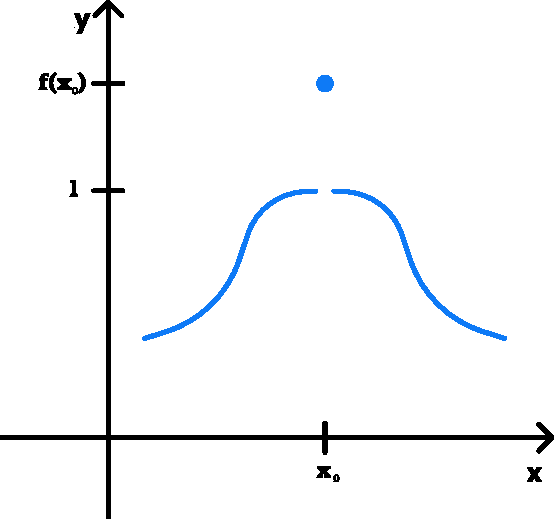
\includegraphics[width=5cm]{./images/discontinuity3.pdf}\hfill
    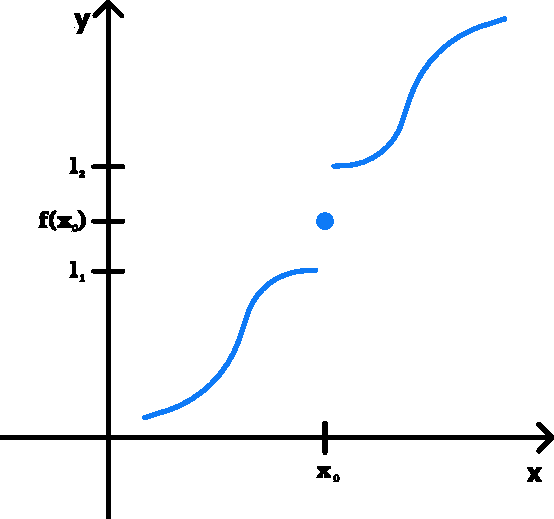
\includegraphics[width=5cm]{./images/discontinuity1.pdf}\hfill
    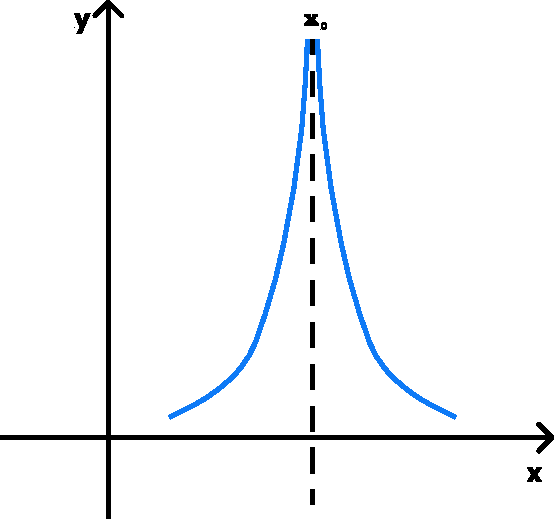
\includegraphics[width=5cm]{./images/discontinuity2.pdf}
\end{figure}

\subsubsection{Esercizio 24}
$f(x) = \frac{\sin(x)}{x}$, $f(x)$ è continua in $0$? \\

\noindent Dato che $D_f: \mathbb{R} - \{0\}$, allora sicuramente $f$ non è continua in $0$ (perché appunto non è definita in quel punto).\\
Cerchiamo quindi di definire una funzione simile a $f(x)$, ma che renda continua $f(x)$:
\begin{equation*}
    g_a(x) = 
    \begin{cases}
        \frac{\sin(x)}{x} \qquad \ se \ x \neq 0\\
        a \qquad \qquad se \ x = 0
    \end{cases}
\end{equation*}

\noindent Ora quindi possiamo calcolare quanto vale la funzione in $0$: $g_a(0) = a$. Dato poi che $\lim_{x \to 0} g_a(x) = 1$, allora l'unico caso in cui $g_a(x)$ è continua in $0$ è quando si ha $g_1(x)$, ovvero quando $a = 1$.\\

\noindent\textbf{NB!} La funzione $g_1(x)$ viene detta \textbf{prolungamento continuo di $f$ in $0$}. Se esiste un prolungamento continuo di un'altra funzione, allora esso è unico. \\

\noindent\textbf{ES.} Sia $f(x) = \frac{1}{|x|}$, siccome $\lim_{x \to 0} \frac{1}{|x|} = +\infty$, allora $f$ non ha prolungamento continuo in $0$ (perché la funzione calcolata in $0$ non può dare di certo come risultato $+\infty$).\\

\noindent\textbf{NB!} Per avere un prolungamento continuo dobbiamo avere una discontinuità eliminabile.

\subsection{Operazioni con funzioni continue}
\subsubsection{Teorema sulla continuità}
Siano $f, g: A \subset \mathbb{R} \xrightarrow{} \mathbb{R}$ e $x_0 \in A$ un punto di accumulazione per $A$. Siano inoltre $f, g$ continue in $x_0$. Allora: $f + g$ e $f \cdot g$ sono continue in $x_0$. Inoltre, se $g(x_0) \neq 0$, allora $\frac{f}{g}$ è continua in $x_0$.\\

\noindent Per dimostrare il precedente teorema basta utilizzare i teoremi della somma, del prodotto, del rapporto insieme alla definizione di continuità.

\subsubsection{Teorema sulla continuità composta}
Sia $f: A \subset \mathbb{R} \xrightarrow{} \mathbb{R}$, $x_0 \in A$ con $x_0$ punto di accumulazione per $A$ e $f$ continua in $x_0$.\\
Sia $g: B \subset \mathbb{R} \xrightarrow{} \mathbb{R}$, $t_0 \in B$ con $t_0$ punto di accumulazione per $B$ e $g$ continua in $t_0$.\\
Inoltre, $g(t_0) = x_0$ (ovvero $\lim_{t \to t_0} g(t) = x_0$ dato che $g$ è continua), allora:
\begin{equation*}
    f \circ g: B \subset \mathbb{R} \xrightarrow{} \mathbb{R} \qquad t \longmapsto f(g(t)) \ continua \ in \ t_0
\end{equation*}

\noindent Per la dimostrazione basta utilizzare il teorema sui limiti per sostituzione. Si noti, inoltre, che dire che $f$ continua in $x_0$ e $g$ continua in $t_0$ è analogo all'\textit{Ipotesi 2.} del teorema sui limiti per sostituzione (perché significa che possiamo calcolare $f(x_0) = \lim_{x \to x_0} f(x)$ e $g(t_0) = \lim_{t \to t_0} g(t)$). \\

\noindent\textbf{ES.} Sia $f(x) = \log|x|$, allora $f(x)$ è continua? \\
\noindent Notiamo subito che $f(x)$ è una funzione composta da $|x|$ (che è continua in $\mathbb{R}$) e $\log(x)$ (che è continua in $(0, +\infty)$. Ciò significa che $\log|x|$ è continua $\forall x \in \mathbb{R} : |x| > 0$, ovvero quando $x \neq 0$.\\

\noindent\textbf{ES.} Sia $f(x) = \sin(e^x)$, allora $f(x)$ è continua?\\
\noindent Notiamo subito che $f(x)$ è una funzione composta da $e^x$ (che abbiamo già verificato essere una funzione continua in $\mathbb{R}$ nella \textit{Proposizione 5}) e $\sin(x)$, che è continua nell'intervallo in cui è definita. Ciò significa che $\sin(e^x)$ è continua $\forall x \in \mathbb{R}$.

\subsubsection{Esercizio 25}
Sia:
\begin{equation*}
    f(x) = \begin{cases}
        \frac{\sin(x)}{x} \qquad \qquad \ \ se \ x > 0 \\
        a \qquad \qquad \qquad \ se \ x = 0 \ con \ a \in \mathbb{R} \\
        \log(1 + |x|) \qquad se \ x < 0
    \end{cases}
\end{equation*}

\noindent Esiste $a \in \mathbb{R}$ tale che $f$ è continua in $\mathbb{R}$?\\

\noindent Sia $x > 0$, allora $f(x) = \frac{\sin(x)}{x}$ è continua $\forall a \in \mathbb{R}$ perché ci troviamo di fronte ad un rapporto di funzioni continue. \\
\noindent Sia $x < 0$, allora $f(x) = \log(1 + |x|)$. Abbiamo quindi $|x|$ (che è continua), $1 + |x|$ (anch'essa continua) e $\log(x)$ (che è continua in $(0, +\infty)$). Dato che $1 + |x| \geq 1$, allora $\log(1 + |x|)$ è continua $\forall x < 0, \forall a \in \mathbb{R}$.\\
\noindent Sia $x = 0$, allora abbiamo che $f(0) = a$. Per la continuità in $0$, $\lim_{x \to 0^+} f(x) = \lim_{x \to 0^-} = f(0)$, ma:
\begin{equation*}
    \lim_{x \to 0^+} \frac{\sin(x)}{x} = 1 \qquad \lim_{x \to 0^-} \log(1 + |x|) = 0
\end{equation*}

\noindent $\implies \nexists \lim_{x \to 0} f(x) \implies f$ non è continua in $0$, $\forall a \in \mathbb{R}$ perché qualunque $a$ scelga, $0 \neq 1$. Si tratta quindi di una discontinuità di prima specie.

\subsubsection{Esercizio 26}
Sia:
\begin{equation*}
    g(x) = \begin{cases}
        \frac{\sin(x)}{x} \qquad \qquad \ \ se \ x > 0 \\
        a \qquad \qquad \qquad \ se \ x = 0 \ con \ a \in \mathbb{R} \\
        \log(b + |x|) \qquad se \ x < 0
    \end{cases}
\end{equation*}

\noindent Per quali valori di $a, b \in \mathbb{R}$, se ne esistono, si ha che $g(x)$ è continua in $\mathbb{R}$?\\

\noindent Per $x \neq 0$ è analogo all'\textit{Esercizio 25}. \\
\noindent Per $x = 0$, allora $g(0) = a$, $\lim_{x \to 0^+} g(x) = 1$ e $\lim_{x \to 0^-} g(x) = \log(b)$. Quindi:
\begin{equation*}
    \exists \lim_{x \to 0} g(x) \iff \begin{cases}
        \log(b) = 1 \ (\lim_{x \to 0^-} g(x) = \lim_{x \to 0^+} g(x)) \\
        b > 0 \ (condizione \ di \ esistenza \ di \ \log(b))
    \end{cases}
    \implies b = e \qquad \forall a \in \mathbb{R}
\end{equation*}

\noindent Allora $f$ è continua in $0$ se e solo se:
\begin{equation*}
    \begin{cases}
        a = \log(b) \ (g(0) = \lim_{x \to 0} g(x)) \\ 
        \log(b) = 1 \\
        b > 0
    \end{cases}
    \implies
    \begin{cases}
        a = 1 \\
        b = e
    \end{cases}
\end{equation*}

\subsection{Teorema della continuità dell'inversa}
Sia $f: I \subset \mathbb{R} \xrightarrow{} \mathbb{R}$ con $I$ intervallo e $f$ strettamente monotona in $I$. Allora $f^{-1}: Imm(f) \xrightarrow{} \mathbb{R}$ è continua su $Imm(f)$.\\

\noindent\textbf{NB!} Non c'è scritto da nessuna parte che $f$ deve essere continua. In altre parole, possono esistere inverse continue di funzioni non continue. \\

\noindent\textbf{NB!} Questo teorema serve per dire che le funzioni trigonometriche inverse sono continue.\\

\noindent\textbf{ES.} Sia:

\begin{equation*}
    f(x) = \begin{cases}
        x - 1 \qquad se \ x \in [0, 1] \\
        x + 1 \qquad se \ x \in (1, 2]
    \end{cases}
    \implies I = [0, 2]
\end{equation*}

\noindent Notiamo che $f(1) = 0$, $\lim_{x \to 1^-} f(x) = 0$ e $\lim_{x \to 1^+} f(x) = 2$ e quindi $f(x)$ non è continua in $1$ perché in $1$ ha una discontinuità di prima specie.\\
\noindent Dimostriamo ora che la funzione è strettamente crescente. Se $x_1 \in [0, 1]$ e $x_2 \in [0, 1]$ con $x_1 < x_2$, allora $f(x_1) = x_1 - 1 < x_2 - 1 = f(x_2)$. Ad esempio, se prendiamo $x_1 = 0$ e $x_2 = 1$, allora si ha che $-1 < 0$.\\
Se invece $x_1 \in (1, 2]$ e $x_2 \in (1, 2]$ con $x_1 < x_2$, allora $f(x_1) = x_1 + 1 < x_2 + 1 = f(x_2)$. Ad esempio, se prendiamo $x_1 = \frac{3}{2}$ e $x_2 = 2$, allora si ha che $\frac{5}{2} < 3$.\\
Infine, se $x_1 \in [0, 1]$ e $x_2 \in (1, 2]$ con $x_1 < x_2$, allora $f(x_1) = x_1 - 1 < x_2 + 1 \implies x_1 - 2 < x_2$. Ad esempio, se prendiamo $x_1 = 0$ e $x_2 = 2$, allora si ha che $-1 < 3$.\\
Consideriamo ora l'immagine della funzione $Imm(f) = [-1, 0] \cup (2, 3]$. Ciò significa che:
\begin{equation*}
    f^{-1}(y) = \begin{cases}
        y + 1 \qquad se \ y \in [-1, 0]\\
        y - 1 \qquad se \ y \in (2, 3]
    \end{cases}
\end{equation*}

\noindent Notiamo quindi come la continuità di $f^{-1}(y)$ dipende dalla continuità dei "rami" ($[-1, 0]$ e $(2, 3]$). Essendo però che sia $y + 1$, che $y - 1$ sono continue, allora anche $f^{-1}(y)$ è continua.\\
In altre parole, la discontinuità della funzione si è tradotta in intervalli disgiunti in cui $f^{-1}(y)$ ha comportamenti differenti a seconda dell'intervallo in cui si trova.

\section{Derivabilità}
\textbf{Def:} Sia $f: I \subset \mathbb{R} \xrightarrow{} \mathbb{R}$, $x_0 \in I$ con $I$ intervallo. Sia $x_0$ \textbf{interno} ad $I$. Sia inoltre $x \in I$ con $x \neq x_0$. Diciamo \textbf{rapporto incrementale di $f$ in $x_0$} la quantità:
\begin{equation*}
    \frac{f(x) - f(x_0)}{x - x_0}
\end{equation*}

\noindent\textbf{NB!} Un punto $x_0$ è interno ad $I$ $\underset{def}{\iff} \exists U_{x_0} \ intorno \ di \ x_0 \ | \ U_{x_0} \subset I$.\\

\noindent\textbf{Def:} Sia $f: I \subset \mathbb{R} \xrightarrow{} \mathbb{R}$, $I$ intervallo, $x_0 \in I$, $x_0$ interno ad $I$. Diremo che $f$ è \textbf{derivabile} in $x_0$ se e solo se: 
\begin{equation*}
    \frac{f(x) - f(x_0)}{x - x_0} = l \in \mathbb{R}
\end{equation*}

\begin{wrapfigure}{r}{0.4\textwidth}
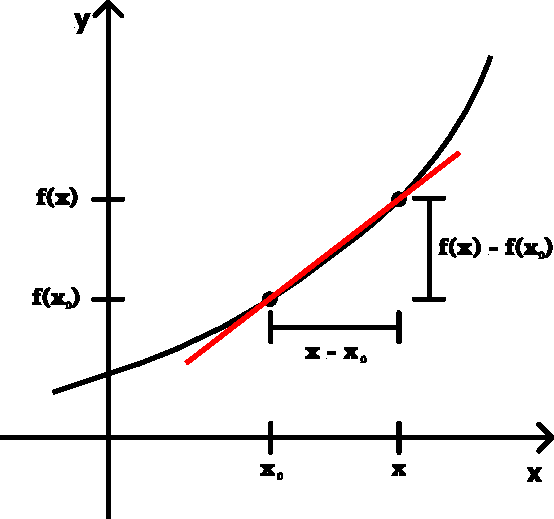
\includegraphics[width=0.9\linewidth]{./images/derivative.pdf}
\end{wrapfigure}

\noindent Si noti che avendo i punti $(x_0, f(x_0))$ e $(x, f(x))$, allora è possibile calcolare il coefficiente della retta, che è proprio pari al rapporto incrementale:
\begin{equation*}
    m = \frac{\Delta y}{\Delta x} = \frac{f(x) - f(x_0)}{x - x_0}
\end{equation*}

\noindent e quindi la retta equivale a $y - f(x_0) = m(x - x_0)$.\\
\noindent In particolare, se facciamo tendere $x$ a $x_0$, allora l'angolo tra la retta $y = f(x_0)$ e la retta $y - f(x_0) = m(x - x_0)$ diminuisce. In altre parole, quando $\lim_{x \to x_0} \frac{f(x) - f(x_0)}{x - x_0} = l \in \mathbb{R}$ vuol dire che $l$ è il coefficiente angolare della retta tangente in $(x_0, f(x_0))$, ovvero la retta può essere scritta come $y - f(x_0) = l(x - x_0)$.\\
Se invece $l = +\infty \ (- \infty)$, allora la retta è tangente, ovvero $x = x_0$ (si ha una retta verticale).

\subsubsection{Notazione delle derivate}
Come le successioni, anche le derivate possono essere scritte secondo diverse notazioni:
\begin{equation*}
    f'(x_0) = l \qquad \frac{d}{dx} f(x_0) \qquad \frac{df}{dx} (x_0)
\end{equation*}

\noindent\textbf{NB!} Le ultime due notazioni \textbf{non} sono frazioni!\\

\noindent\textbf{Teorema:} Sia $f: I \subset \mathbb{R} \xrightarrow{} \mathbb{R}$, $I$ intervallo e $x_0 \in I$ con $x_0$ interno ad $I$. Quindi se $f$ è derivabile in $x_0$, allora $f$ è continua in $x_0$.\\

\noindent\textbf{NB!} Il teorema qui sopra \textbf{non} vale al contrario, ovvero \textbf{non} è vero che se $f$ è continua, allora $f$ è derivabile.\\

\noindent Dimostriamo il teorema qui sopra:
\begin{equation*}
    \lim_{x \to x_0} (f(x) - f(x_0)) = \lim_{x \to x_0} \frac{f(x) - f(x_0)}{x - x_0} \cdot (x - x_0) = 0
\end{equation*}

\noindent dato che $(x - x_0) \to 0$ e, per ipotesi, $\frac{f(x) - f(x_0)}{x - x_0} = f'(x_0) \in \mathbb{R}$.\\

\noindent Come detto precedentemente, il viceversa non vale. Infatti, sia $f(x) = |x|$. Sappiamo che $f(x)$ è continua in $0$ perché $f(0) = \lim_{x \to 0} f(x) = 0$, ma:
\begin{equation*}
    \lim_{x \to 0^+} \frac{f(x) - f(0)}{x - 0} = \lim_{x \to 0^+} \frac{|x|}{x} = \lim_{x \to 0^+} \frac{x}{x} = 1
\end{equation*}
\begin{equation*}
    \lim_{x \to 0^-} \frac{f(x) - f(0)}{x - 0} = \lim_{x \to 0^-} \frac{|x|}{x} = \lim_{x \to 0^-} \frac{-x}{x} = -1
\end{equation*}

\noindent (nel primo caso, essendo $x > 0$, si ha che $|x| = x$; mentre nel secondo, $x < 0$ e quindi $|x| = -x$). La funzione quindi non è derivabile in $0$ (perché i due limiti sono diversi), ma è continua.

\subsection{Punti di non derivabilità}
\textbf{Def:} Sia $f: I \xrightarrow{} \mathbb{R}$, $I$ intervallo, $x_0 \in I$ e $x_0$ interno ad $I$. Allora:
\begin{enumerate}
    \item se $\lim_{x \to x_0^+} \frac{f(x) - f(x_0)}{x - x_0} = l_1 \in \mathbb{R}$, $\lim_{x \to x_0^-} \frac{f(x) - f(x_0)}{x - x_0} = l_2 \in \mathbb{R}$ e $l_1 \neq l_2$, allora $x_0$ è detto \textbf{punto angoloso}.
    \item se uno tra $\lim_{x \to x_0^+} \frac{f(x) - f(x_0)}{x - x_0}$ e $\lim_{x \to x_0^-} \frac{f(x) - f(x_0)}{x - x_0}$ è $+\infty \ (-\infty)$, allora $x_0$ è detto \textbf{punto cuspidale}
\end{enumerate}

\noindent\textbf{ES.} $0$ è punto angoloso per $|x|$.\\

\noindent\textbf{ES.} Sia 
\begin{equation*}
    g(x) = \sqrt{|x|} = \begin{cases}
        \sqrt{x} \qquad \ \ se \ x \geq 0\\
        \sqrt{-x} \qquad se \ x < 0
    \end{cases}
\end{equation*}

\noindent Calcoliamo ora il rapporto incrementale:
\begin{equation*}
    \lim_{x \to 0^+} \frac{g(x) - g(0)}{x - 0} = \lim_{x \to 0^+} \frac{\sqrt{x}}{x} = \lim_{x \to 0^+} \frac{1}{\sqrt{x}} = +\infty
\end{equation*}

\noindent Basterebbe questo per dire che $0$ è punto cuspidale per $g(x)$, ma calcoliamo anche il limite sinistro:
\begin{equation*}
    \lim_{x \to 0^-} \frac{g(x) - g(x_0)}{x - 0} = \lim_{x \to 0^-} \frac{\sqrt{-x}}{-x} = \lim_{x \to 0^-} -\left(\frac{\sqrt{-x}}{-x}\right) = - \lim_{x \to 0^-} \frac{1}{\sqrt{-x}} = -\infty
\end{equation*}

\noindent\textbf{NB!} Abbiamo dovuto "inserire" un "-" perché per semplificare l'espressione dobbiamo avere una quantità positiva e quindi $x < 0 \implies -x > 0$.

\subsection{Insieme di continuità/derivabilità}
\textbf{Def:} Sia $f: A \subset \mathbb{R} \xrightarrow{} \mathbb{R}$. Chiamiamo ora il dominio di continuità di $f$ $D(f)^{CONT} = \{x \in A \ | \ f \ continua \ in \ x \}$ e il dominio di derivabilità di $f$ $D(f)^{DER} = \{x \in A \ | \ f \ derivabile \ in \ x \}$.\\
Chiaramente, si ha che $D(f)^{DER} \subsetneq D(f)^{CONT} \subset A$ (sempre per il fatto che una funzione derivabile è sicuramente continua, ma non vale il viceversa).\\

\noindent\textbf{Funzione derivata prima - Def:} Sia $f: I \subset \mathbb{R} \xrightarrow{} \mathbb{R}$, $I$ intervallo, $f$ derivabile in $I$ (ovvero $D(f)^{DER} = I$).\\
Definiamo la funzione derivata prima di $f$: 
\begin{equation*}
    g: D(f)^{DER} \xrightarrow{} \mathbb{R} \qquad x \longmapsto f'(x)
\end{equation*}

\noindent dove $x$ è un punto di derivabilità di $f$ (ovvero esiste $f'(x)$). Usualmente scriviamo che $g = f'$ (possiamo anche scrivere $f^{(1)} = f'$ oppure che $f^{(0)} = f$).

\subsection{Derivabilità delle funzioni fondamentali}
\subsubsection{Funzioni costanti}
Sia $f(x) = c \qquad \forall x \in \mathbb{R}, c \in \mathbb{R}$, allora $f(x)$ è derivabile in $\mathbb{R}$ e $f'(x) = 0 \qquad \forall x \in \mathbb{R}$.\\
È molto semplice da dimostrare: prendiamo un punto $x$ fissato del dominio, allora:
\begin{equation*}
    \lim_{t \to x} \frac{f(t) - f(x)}{t - x} = \lim_{t \to x} \frac{c - c}{t - x} = 0
\end{equation*}

\noindent (dato che $c - c = 0$, mentre $t - x \in \mathbb{R}$ e $t - x \neq 0$ perché stiamo lavorando in intorni bucati di $x$, cioè l'espressione vale $\forall t \neq x$.

\subsubsection{Funzioni potenza con esponente naturale}
Sia $f(x) = x^n \qquad n \in \mathbb{N} - \{0\}$. Allora $f'(x) = nx^{n - 1} \qquad \forall x \in \mathbb{R}, \forall n \geq 1$.\\

\noindent Dimostriamo ora il significato della formula di derivazione. Se $n = 1$, allora $f(x) = x$ e si ha che:
\begin{equation*}
    \lim_{t \to x} \frac{f(t) - f(x)}{t - x} = \lim_{t \to x} \frac{t - x}{t - x} = 1 \qquad \forall x \in \mathbb{R}
\end{equation*}

\noindent Prendiamo ora il caso $n \geq 2$ e poniamo la sostituzione $t = x + h$, allora:
\begin{equation*}
    \lim_{t \to x} \frac{f(t) - f(x)}{t - x} = \lim_{h \to 0} \frac{f(x + h) - f(x)}{h} = \lim_{h \to 0} \frac{(x + h)^n - x^n}{h} = \lim_{h \to 0} \frac{x^n\left[\left(\dfrac{x + h}{x}\right)^n - 1\right]}{h} =
\end{equation*}
\begin{equation*}
    = \lim_{h \to 0} \frac{x^n\left[\left(1 + \dfrac{h}{x}\right)^n - 1\right]}{h} \overset{x \neq 0}{\implies} x^n \lim_{h \to 0} \frac{\left[\left(1 + \dfrac{h}{x}\right)^n - 1\right]}{\frac{h}{x}} \cdot \frac{1}{x} = x^{n - 1} \lim_{h \to 0} \frac{\left[\left(1 + \dfrac{h}{x}\right)^n - 1\right]}{\frac{h}{x}}
\end{equation*}

\noindent Effettuiamo la sostituzione $s = \frac{h}{x}$ e otteniamo:
\begin{equation*}
    x^{n - 1} \lim_{s \to 0} \frac{(1 + s)^n - 1}{s} = nx^{n - 1} \ con \ x \neq 0
\end{equation*}

\noindent Se invece $x = 0$ e $n \geq 2$, allora:
\begin{equation*}
    \lim_{h \to 0} \frac{f(0 + h) - f(0)}{h} = \lim_{h \to 0} \frac{h^n - 0}{h} = \lim_{h \to 0} h^{n - 1} = 0
\end{equation*}

\noindent ($\lim_{h \to 0} h^{n - 1} = 0$ perché $n - 1 \geq 1$). Abbiamo quindi dimostrato che $(x^n)' = nx^{n - 1} \qquad \forall x \in \mathbb{R}, \forall n \geq 1$.

\subsubsection{Funzioni potenza con esponente reale}
Sia $x > 0$, $u \in \mathbb{R}$, allora se abbiamo $f(x) \vcentcolon = e^{u\log(x)} \implies f'(x) = ux^{u - 1} \qquad \forall x > 0, \forall u \in \mathbb{R}$.\\

\noindent Per dimostrarlo, utilizziamo gli stessi passaggi svolti precedentemente:
\begin{align*}
    \lim_{h \to 0} \frac{f(x + h) - f(x)}{h} &= \lim_{h \to 0} \frac{(x + h)^u - x^u}{h} = \lim_{h \to 0} \frac{x^u\left[\left(1 + \dfrac{h}{x}\right)^u - 1\right]}{h} = x^u \lim_{h \to 0} \frac{\left(1 + \dfrac{h}{x}\right)^u - 1}{\frac{h}{x}} \cdot \frac{1}{x} \\
    &= x^{u - 1} \lim_{v \to 0} \frac{(1 + v)^u - 1}{v} = ux^{u - 1}
\end{align*}

\subsubsection{Funzioni esponenziali}
Sia $f(x) = a^x$, allora $f'(x) = a^x\log(a) \qquad \forall x \in \mathbb{R}, a > 0$.\\

\noindent Dimostrazione:
\begin{equation*}
    \lim_{h \to 0} \frac{f(x + h) - f(x)}{h} = \lim_{h \to 0} \frac{a^{x + h} - a^x}{h} = a^x \lim_{h \to 0} \frac{a^h - 1}{h} = a^x\log(a)
\end{equation*}

\noindent\textbf{NB!} Un caso particolare di queste funzioni è quando $a = e$, per cui si ha che: $f(x) = e^x \implies f'(x) = e^x \qquad \forall x \in \mathbb{R}$.

\subsubsection{Funzioni seno e coseno}
Sia $f(x) = \sin(x)$, allora $f'(x) = \cos(x) \qquad \forall x \in \mathbb{R}$. \\

\noindent Dimostriamo la precedente regola di derivazione sfruttando la prostaferesi:
\begin{align*}
    \lim_{h \to 0} \frac{\sin(x + h) - \sin(x)}{h} &= \lim_{h \to 0}\frac{2\cos\left(\dfrac{x + h + x}{2}\right)\sin\left(\dfrac{x + h - x}{2}\right)}{h} = \lim_{h \to 0} \frac{2\cos\left(x + \dfrac{h}{2}\right)\sin\left(\dfrac{h}{2}\right)}{h}\\
    &= \lim_{h \to 0} \frac{\sin\left(\dfrac{h}{2}\right)}{\frac{h}{2}}\cos\left(x + \frac{h}{2}\right) = \cos(x)
\end{align*}

\noindent Sia $f(x) = \cos(x)$, allora $f'(x) = -\sin(x) \qquad \forall x \in \mathbb{R}$. \\

\noindent Dimostriamo la precedente regola di derivazione sfruttando la prostaferesi:
\begin{align*}
    \lim_{h \to 0} \frac{\cos(x + h) - \cos(x)}{h} &= \lim_{h \to 0}\frac{-2\sin\left(\dfrac{x + h + x}{2}\right)\sin\left(\dfrac{x + h - x}{2}\right)}{h} = \lim_{h \to 0} \frac{-2\sin\left(x + \dfrac{h}{2}\right)\sin\left(\dfrac{h}{2}\right)}{h}\\
    &= \lim_{h \to 0} - \frac{\sin\left(\dfrac{h}{2}\right)}{\frac{h}{2}}\sin\left(x + \frac{h}{2}\right) = -\sin(x)
\end{align*}

\noindent\textbf{Link:} \href{https://www.youmath.it/formulari/65-formulari-di-trigonometria-logaritmi-esponenziali/1048-formule-di-prostaferesi.html}{Formule di prostaferesi}.

\subsubsection{Funzioni logaritmiche}
Sia $x > 0$, $a > 0$ con $a \neq 1$ e $f(x) = \log_a(x)$, allora $f'(x) = \frac{1}{x} \log_a(e) \qquad \forall x > 0$.\\

\noindent Dimostriamo ora la precedente regola di derivazione. Riscriviamo il rapporto incrementale, ponendo $x + h = x(1 + \frac{h}{x})$, dato che $x$ è positivo:
\begin{align*}
    \lim_{h \to 0} \frac{f(x + h) - f(x)}{h} &= \lim_{h \to 0} \frac{\log_a(x + h) - \log_a(x)}{h} = \lim_{h \to 0} \frac{\log_a\left(x\left(1 + \dfrac{h}{x}\right)\right) - \log_a(x)}{h}\\
    &= \lim_{h \to 0} \frac{\log_a(x) + \log_a\left(1 + \dfrac{h}{x}\right) - \log_a(x)}{h} = \lim_{h \to 0} \frac{\log_a\left(1 + \dfrac{h}{x}\right)}{\frac{h}{x}} \cdot \frac{1}{x} \\
    &= \frac{1}{x} \lim_{t \to 0}\frac{\log_a(1 + t)}{t} = \frac{1}{x} \log_a(e)
\end{align*}

\noindent\textbf{NB!} Abbiamo potuto compiere operazioni su $x + h$ solo perché abbiamo posto che $h > -x$, altrimenti il logaritmo non sarebbe stato definito.\\

\noindent\textbf{Osservazione:} $(log(e))' = \frac{1}{x} \qquad \forall x > 0$.\\

\noindent\textbf{Osservazione:} $(\log|x|)' = \frac{1}{x} \qquad \forall x \neq 0$ (e non $\frac{1}{|x|}$).\\
Innanzitutto, sappiamo che $D_f: \mathbb{R} - \{0\}$ e riscriviamo la funzione:
\begin{equation*}
    \log|x| = \begin{cases}
        \log(x) \qquad \ \ se \ x > 0 \\
        \log(-x) \qquad se \ x < 0
    \end{cases}
\end{equation*}

\noindent Sia ora $x < 0$ e $(h + x) < 0$, allora:
\begin{equation*}
    \lim_{h \to 0} \frac{\log(-(x + h)) - \log(-x)}{h} = \lim_{h \to 0} \frac{\log(-x - h) - \log(-x)}{h}
\end{equation*}

\noindent Raccogliamo ora $-x$ ed otteniamo che $-x - h = -x(1 + \frac{h}{x})$ che è sicuramente positivo dato che $1 + \frac{h}{x} = \frac{x + h}{x}$, che è il rapporto tra due quantità negative. Possiamo quindi calcolare il logaritmo senza problemi:
\begin{equation*}
    = \lim_{h \to 0} \frac{\log(-x) + \log\left(1 + \dfrac{h}{x}\right) - \log(-x)}{h} = \lim_{h \to 0} \frac{\log\left(1 + \dfrac{h}{x}\right)}{\frac{h}{x}} \cdot \frac{1}{x} 
\end{equation*}

\noindent e quindi per $x < 0$ risulta:
\begin{equation*}
    \lim_{h \to 0} \frac{\log|x + h| - \log|x|}{h} = \frac{1}{x} \lim_{h \to 0} \frac{\log\left(1 + \dfrac{h}{x}\right)}{\frac{h}{x}} = \frac{1}{x} \qquad \forall x \in \mathbb{R} \implies (\log|x|)' = \frac{1}{x} \qquad \forall x \neq 0
\end{equation*}

\noindent\textbf{Teorema:} Siano $f, g: I \subset \mathbb{R} \xrightarrow{} \mathbb{R}$, $I$ intervallo, $x_0 \in I$, $x_0$ interno ad $I$ e $f, g$ derivabili in $x_0$. Allora $f + g$ e $f \cdot g$ sono derivabili in $x_0$ e, se $g(x_0) \neq 0$, allora $\frac{f}{g}$ è derivabile in $x_0$. Inolte:
\begin{enumerate}
    \item $(f + g)'(x_0) = f'(x_0) + g'(x_0)$;
    \item $(f \cdot g)'(x_0) = f'(x_0)g(x_0) + f(x_0)g'(x_0)$;
    \item $\left(\dfrac{f}{g}\right)'(x_0) = \dfrac{f'(x_0)g(x_0) - f(x_0)g'(x_0)}{(g(x_0))^2}$.
\end{enumerate}

\noindent Dimostriamo ora il punto 2, aggiungendo e togliendo $f(x_0)g(x)$:
\begin{align*}
    \lim_{x \to x_0} \frac{(f \cdot g)(x) - (f \cdot g)(x_0)}{x - x_0} &= \lim_{x \to x_0} \frac{f(x)g(x) - f(x_0)g(x_0) - f(x_0)g(x) + f(x_0)g(x)}{x - x_0}\\
    &= \lim_{x \to x_0} \left(\frac{f(x) - f(x_0)}{x - x_0} \cdot g(x)\right) + \lim_{x \to x_0} \left(\frac{g(x) - g(x_0)}{x - x_0}\right) f(x_0)
\end{align*}

\noindent Ora dato che $g(x)$ è derivabile, allora è continua e quindi possiamo scrivere che $\lim_{x \to x_0} g(x) = g(x_0)$. Pertanto si ha che:
\begin{equation*}
    \lim_{x \to x_0} \frac{(f \cdot g)(x) - (f \cdot g)(x_0)}{x - x_0} = f'(x_0)g(x_0) + f(x_0)g'(x_0)
\end{equation*}

\noindent\textbf{ES.} Derivata di una funzione moltiplicata per una costante: $(cf)'(x_0) = cf'(x_0) + 0 \cdot f(x_0) = cf'(x_0) \qquad \forall x_0 \in D(f)^{DER}$.\\

\noindent\textbf{ES.} Derivata della somma di due funzioni moltiplicate per una costante: $(af + bg)'(x_0) = af'(x_0) + bg'(x_0) \qquad \forall a, b \in \mathbb{R}, \forall x_0 \in (D(f)^{DER} \cap D(g)^{DER})$. Infatti, basterebbe calcolare $(af)'(x_0)$ e $(bf)'(x_0)$.\\

\noindent\textbf{ES.} Derivata di un polinomio. Si noti che il passaggio dalla prima sommatoria alla seconda altro non è che dire che la derivata del polinomio è uguale alla somma delle singole derivate dei monomi. Nel terzo passaggio viene portata fuori $a_k$ essendo una costante che non influisce nel calcolo della derivata.
\begin{equation*}
    (p(x))' = \left(\sum_{k = 0}^n a_k x^k\right)' = \sum_{k = 0}^n(a_kx^k)' = \sum_{k = 0}^n a_k(x^k)' = \sum_{k = 0}^n a_k k x^{k - 1} \qquad \forall x \in \mathbb{R}, \forall a_k \in \mathbb{R}
\end{equation*}

\noindent Abbiamo ottenuto un polinomio di grado massimo $n - 1$. Ora dato che quando $k = 0$, l'argomento della sommatoria vale $0$, possiamo scrivere direttamente:
\begin{equation*}
    (p(x))' = \sum_{k =1}^n a_k k x^{k - 1} \qquad \forall x \in \mathbb{R}, \forall a_k \in \mathbb{R}
\end{equation*}

\noindent\textbf{ES.} Derivata di una potenza negativa. Sia $x \neq 0$ e $n \geq 1, n \in \mathbb{N}$, allora se $f(x) = x^{-n}$, si ha che:
\begin{equation*}
    (f(x))' = \left(\frac{1}{x^n}\right)' = \frac{(1)'x^n - 1 \cdot nx^{n - 1}}{x^{2n}} = -n \cdot \frac{x^{n - 1}}{x^{2n}} = - \frac{n}{x^{n + 1}} = -nx^{-n - 1} \qquad (x \neq 0)
\end{equation*} 

\subsection{Teorema del differenziale di Lagrange}
Sia $f: I \subset \mathbb{R} \xrightarrow{} \mathbb{R}$, $I$ intervallo, $x_0 \in I$ e $x_0$ interno ad $I$, $f$ derivabile in $x_0$. Allora $\exists \omega: I \xrightarrow{} \mathbb{R}$ tale che $\omega$ è continua in $x_0$, $\omega(x_0) = 0$ e:
\begin{equation*}
    f(x) = f(x_0) + f'(x_0)(x - x_0) + \omega(x)(x - x_0)
\end{equation*}

\noindent\textbf{NB!} La prima parte della tesi qui sopra ($f(x_0) + f'(x_0)(x - x_0)$) è un polinomio di primo grado, che rappresenta l'equazione della retta tangente a $(x_0, f(x_0))$, mentre la seconda parte ($\omega(x)(x - x_0)$) è un altro polinomio moltiplicato ad un qualcosa che tende a $0$ ($x - x_0)$ più velocemente rispetto alla prima parte della tesi. In altre parole, la tesi "approssima" $f(x)$ (prima parte) con un "errore" che tende a $0$ più velocemente di $x - x_0$ (seconda parte), infatti:
\begin{equation*}
    \lim_{x \to x_0} \frac{\omega(x)(x - x_0)}{x - x_0} = \lim_{x \to x_0} \omega(x) = \omega(x_0) = 0
\end{equation*}

\subsubsection{Dimostrazione del teorema del differenziale di Lagrange}
Sia:
\begin{equation*}
    \omega(x) \vcentcolon = \begin{cases}
        \dfrac{f(x) - f(x_0)}{x - x_0} - f'(x_0) \qquad se \ x \neq x_0\\
        0 \qquad \qquad \qquad \qquad \qquad \quad \ se \ x = x_0
    \end{cases}
\end{equation*}

\noindent Verifichiamo che la funzione sia continua:
\begin{equation*}
    \lim_{x \to x_0} \omega(x) = \lim_{x \to x_0} \frac{f(x) - f(x_0)}{x - x_0} - f'(x_0) = f'(x_0) - f'(x_0) = 0 = \omega(x_0)
\end{equation*}

\noindent Sia ora $x \neq x_0$:
\begin{equation*}
    \omega(x) = \frac{f(x) - f(x_0)}{x - x_0} - f'(x_0) \iff \omega(x) + f'(x_0) = \frac{f(x) - f(x_0)}{x - x_0}
\end{equation*}
\begin{equation*}
    (\omega(x) + f'(x_0))(x - x_0) = f(x) - f(x_0) \implies f(x) = f(x_0) + f'(x_0)(x - x_0) + \omega(x)(x - x_0)
\end{equation*}

\noindent Abbiamo quindi ottenuto la stessa formula della tesi, ma al momento vale solo $\forall x \in I, x \neq x_0$. Consideriamo ora il caso $x = x_0$, allora si ha che:
\begin{equation*}
    f(x_0) = f(x_0) + f'(x_0)(x_0 - x_0) + \omega(x_0)(x_0 - x_0) \implies f(x_0) = f(x_0)
\end{equation*}

\noindent Perciò, il teorema del differenziale di Lagrange vale $\forall x \in I$.

\subsubsection{Teorema (opposto del teorema del differenziale di Lagrange)}
Sia $f: I \subset \mathbb{R} \xrightarrow{} \mathbb{R}$, $I$ intervallo, $x_0$ interno ad $I$. Sia $a \in \mathbb{R}$ e $\omega: I \xrightarrow{} \mathbb{R}$ tali che $\omega(x_0) = 0$, $\omega$ è continua in $x_0$ e si ha che:
\begin{equation*}
    f(x) = f(x_0) + a(x - x_0) + \omega(x)(x - x_0) \qquad \forall x \in I
\end{equation*}

\noindent Allora $f$ è derivabile in $x_0$ e $f'(x_0) = a$.\\

\noindent Dimostriamo ora il precedente teorema. Sia $x \neq x_0$, $x \in I$, allora:
\begin{equation*}
    \lim_{x \to x_0} \frac{f(x) - f(x_0)}{x - x_0} = \lim_{x \to x_0} \frac{a(x - x_0) + \omega(x)(x - x_0)}{x - x_0} = \lim_{x \to x_0} (a + \omega(x)) = a + \omega(x_0) = a
\end{equation*}

\noindent Quindi $f$ è derivabile in $x_0$ e $f'(x_0) = a$.

\subsection{Teorema della derivata delle funzioni composte}
Sia $f: I \subset \mathbb{R} \xrightarrow{} \mathbb{R}$, $I$ intervallo, $t_0 \in I$, $t_0$ interno ad $I$, $f$ derivabile in $t_0$.\\
Sia $g: J \subset \mathbb{R} \xrightarrow{} I$, $J$ intervallo, $x_0 \in J$, $x_0$ interno a $J$, $g$ derivabile in $x_0$ e $g(x_0) = t_0$. Allora $f \circ g: J \xrightarrow{} \mathbb{R}$ è derivabile in $x_0$ e:
\begin{equation*}
    (f \circ g)'(x_0) = f'(t_0)g'(x_0) \qquad [= f'(g(x))g'(x)]
\end{equation*}

\subsubsection{Dimostrazione del teorema della derivata delle funzioni composte}
Per il teorema del differenziale su $f$: $\exists \omega$ continua in $t_0$, $\omega(t_0) = 0$ tale che:
\begin{equation*}
    f(t) = f(t_0) + f'(t_0)(t - t_0) + \omega(t)(t - t_0) \qquad \forall t \in I
\end{equation*}

\noindent Sia $t \in Imm(g) \subset I$ (cioè $\exists x \in J \ | \ g(x) = t$). Ricordiamo, inoltre, che $g(x_0) = t_0$, allora:
\begin{equation*}
    f(g(x)) = f(g(x_0)) + f'(g(x_0))(g(x) - g(x_0)) + \omega(g(x))(g(x) - g(x_0)) \qquad \forall x \in J
\end{equation*}

\noindent Quindi:
\begin{align*}
    \lim_{x \to x_0} \frac{f(g(x)) - f(g(x_0))}{x - x_0} &= \lim_{x \to x_0} \frac{f'(g(x_0))(g(x) - g(x_0)) + \omega(g(x))(g(x) - g(x_0))}{x - x_0}\\
    &= f'(g(x_0)) \lim_{x \to x_0} \frac{g(x) - g(x_0)}{x - x_0} + \lim_{x \to x_0} \omega(g(x)) \cdot \frac{g(x) - g(x_0)}{x - x_0}
\end{align*}

\noindent Dato che $\lim_{x \to x_0} \frac{g(x) - g(x_0)}{x - x_0} = g'(x_0)$ e che $\lim_{x \to x_0} \omega(g(x)) = \omega(g(x_0)) = \omega(t_0) = 0$, allora:
\begin{equation*}
    f'(g(x_0)) \lim_{x \to x_0} \frac{g(x) - g(x_0)}{x - x_0} + \lim_{x \to x_0} \omega(g(x)) \cdot \frac{g(x) - g(x_0)}{x - x_0} = f'(g(x_0))g'(x_0) \in \mathbb{R}
\end{equation*}

\noindent Possiamo quindi concludere che $f \circ g$ è derivabile in $x_0$ e $(f \circ g)'(x_0) = f'(g(x))g'(x_0)$.\\

\noindent\textbf{ES.} $f(x) = \sin(e^{2x} + 2)$ con $x \in \mathbb{R}$. \\
Sappiamo che $e^x$ è derivabile e lo stesso vale per $2x$, per cui $e^{2x}$ è derivabile per composizione di funzioni derivabili.\\
$e^{2x} + 2$ rimane poi comunque derivabile perché stiamo sommando due funzioni derivabili. \\
Infine, $f(x)$ è anch'essa derivabile nel suo dominio perché si tratta di una composizione di funzioni derivabili.\\
Partiamo quindi dalla funzione più esterna per calcolare la derivata. Sia $h(g(x)) = \sin(e^{2x} + 2)$, allora:
\begin{equation*}
    (h(g(x)))' = h'(g(x))g'(x) = \cos(g(x)) g'(x)
\end{equation*}

\noindent Sia ora $g(x) = e^{2x} + 2 = l(m(x))$ dove $l(u) = e^u + 2$ e $m(x) = 2x$, allora:
\begin{equation*}
    g'(x) = l'(m(x)) m'(x) = e^{(m(x))}m'(x) = e^{2x} \cdot 2 = 2e^{2x}
\end{equation*}

\noindent Unendo tutti i risultati, otteniamo quindi:
\begin{equation*}
    \implies (\sin(e^{2x} + 2))' = 2\cos(e^{2x} + 2)e^{2x}
\end{equation*}

\noindent\textbf{NB!} Quando si effettua l'analisi della derivabilità, si parte sempre dalla funzione più interna; quando si effettua il calcolo della derivata di una funzione composta, si parte sempre dalla funzione più esterna.

\subsection{Teorema della derivata dell'inversa}
Sia $f: I \subset \mathbb{R} \xrightarrow{} \mathbb{R}$, $I$ intervallo, $x_0 \in I$, $x_0$ interno ad $I$, $f$ derivabile in $x_0$. Sia $f'(x_0) \neq 0$ e $f$ strettamente monotona in $I$. Allora $f^{-1}: Imm(f) \xrightarrow{} I$ è derivabile in $y_0 = f(x_0)$ e si ha che:
\begin{equation*}
   (f^{-1})(y_0) = \frac{1}{f'(x_0)}
\end{equation*}

\subsubsection{Esempi di derivate dell'inversa}
\textbf{Derivata dell'inversa del seno}\\
Sia $f(t) = \sin(t)$, $f: [-\frac{\pi}{2}, \frac{\pi}{2}] \xrightarrow{} [-1, 1] \implies g(x) = \arcsin(x)$, $g: [-1, 1] \xrightarrow{} [-\frac{\pi}{2}, \frac{\pi}{2}]$.\\
Per ipotesi $f(t)$ è derivabile e $f'(t) \neq 0$. Dato che $f'(t) = (\sin(t))' = \cos(t) \neq 0 \implies t \in (-\frac{\pi}{2}, \frac{\pi}{2})$. Per il teorema della derivata inversa, $g$ è derivabile nell'intervallo $(- 1, 1)$. Inoltre, si ha che:
\begin{equation*}
    (\arcsin(x))' = \frac{1}{\cos(\arcsin(x))} \qquad con \ x \in (-1, 1)
\end{equation*}

\noindent Ora, dato che $x \in (-1, 1)$, allora $\arcsin(x) \in (-\frac{\pi}{2}, \frac{\pi}{2})$, il che significa che $\cos(\arcsin(x)) > 0$. \\
Visto che $\sqrt{y^2} = |y|$ e che $|y| = y$ se $y > 0$, allora possiamo dire che:
\begin{equation*}
    \cos(\arcsin(x)) = \sqrt{(\cos(\arcsin(x))^2}
\end{equation*}

\noindent Per il teorema di Pitagora ($\cos^2(x) + \sin^2(x) = 1$), otteniamo che:
\begin{equation*}
    \sqrt{(\cos(\arcsin(x))^2} = \sqrt{1 - (\sin(\arcsin(x))^2} = \sqrt{1 - x^2} \implies (\arcsin(x))' = \frac{1}{\sqrt{1 - x^2}} \quad con \ x \in (-1, 1)
\end{equation*}

\noindent\textbf{Derivata dell'inversa del coseno}\\
Sia $f(t) = \cos(t)$, $f: [0, \pi] \xrightarrow{} [-1, 1] \implies g(x) = \arccos(x)$, $g: [-1, 1] \xrightarrow{} [0, \pi]$.\\
Per ipotesi $f(t)$ è derivabile e $f'(t) \neq 0$. Dato che $f'(t) = (\cos(t))' = -\sin(t) \neq 0 \implies t \in (0, \pi)$. Per il teorema della derivata inversa, $g$ è derivabile nell'intervallo $(- 1, 1)$. Inoltre, si ha che:
\begin{equation*}
    (\arccos(x))' = -\frac{1}{\sin(\arccos(x))} \qquad con \ x \in (-1, 1)
\end{equation*}

\noindent Ora, dato che $x \in (-1, 1)$, allora $\arccos(x) \in (0, \pi)$, il che significa che $\sin(\arccos(x)) > 0$. \\
Visto che $\sqrt{y^2} = |y|$ e che $|y| = y$ se $y > 0$, allora possiamo dire che:
\begin{equation*}
    \sin(\arccos(x)) = \sqrt{(\sin(\arccos(x))^2}
\end{equation*}

\noindent Per il teorema di Pitagora ($\cos^2(x) + \sin^2(x) = 1$), otteniamo che:
\begin{equation*}
    \sqrt{(\sin(\arccos(x))^2} = \sqrt{1 - (\cos(\arccos(x))^2} = \sqrt{1 - x^2} \implies (\arccos(x))' = -\frac{1}{\sqrt{1 - x^2}} \qquad con \ x \in (-1, 1)
\end{equation*}

\noindent\textbf{Derivata dell'inversa della tangente}\\
Sia $f(t) = \tan(t)$, $f: (-\frac{\pi}{2}, \frac{\pi}{2}) \xrightarrow{} \mathbb{R} \implies g(x) = \arctan(x)$, $g: \mathbb{R} \xrightarrow{} (-\frac{\pi}{2}, \frac{\pi}{2})$ (di per sé, la tangente non sarebbe invertibile, ma l'abbiamo resa tale restringendo il dominio).\\
Per ipotesi $f(t)$ è derivabile e $f'(t) \neq 0$. Dato che $f'(t) = (\tan(t))' = \left(\frac{\sin(t)}{\cos(t)}\right)'= \frac{\cos^2(t) + \sin^2(t)}{\cos^2(t)} = \frac{1}{\cos^2(t)} = 1 + \tan^2(t) \geq 1 > 0 \implies t \in (-\frac{\pi}{2}, \frac{\pi}{2})$. Per il teorema della derivata inversa, $g$ è derivabile in $\mathbb{R}$ e si ha che:
\begin{equation*}
    (\arctan(x))' = \frac{1}{1 + (\tan(\arctan(x))^2} = \frac{1}{1 + x^2} \qquad con \ x \in (-1, 1)
\end{equation*}

\noindent\textbf{Ricavare la derivata del $\log(x)$}\\
Sia $g(x) = \log(x)$ con $x > 0$. Come sappiamo, il logaritmo è la funzione inversa dell'esponenziale $f(t) = e^t$, per cui vale $f'(t) = e^t$. Non avendo delle restrizioni sulla derivabilità della funzione inversa, possiamo utilizzare il teorema della derivata dell'inversa:
\begin{equation*}
    g'(x) = \frac{1}{e^{\log(x)}} = \frac{1}{x} \qquad con \ x > 0
\end{equation*}

\noindent\textbf{Ricavare la derivata di una radice}\\
Sia $g: I \xrightarrow{} I$, che associa $x \longmapsto x^{\frac{1}{n}}$, con $I$ che può quindi essere $I = [0, +\infty)$ se $n$ è pari oppure $I = \mathbb{R}$ se $n$ è dispari. Capiamo quindi che $g$ è l'inversa di $f: I \xrightarrow{} I$, che associa $t \longmapsto t^n$.\\
Dato che $f$ è derivabile in $I$ e $f'(t) = nt^{n - 1} \neq 0 \qquad \forall t \neq 0$, allora $g$ è derivabile per $x \in I$ tale che $x = t^n$, $f'(t) \neq 0$, cioè $g$ è derivabile per $x \in I - \{0\}$. Inoltre, si ha che:
\begin{equation*}
    g'(x) =(x^{\frac{1}{n}})' = \frac{1}{f'(x^{\frac{1}{n}})} = \frac{1}{n(x^{\frac{1}{n}})^{n-1}} = \frac{1}{nx^{1 - \frac{1}{n}}} = \frac{1}{n} x^{\frac{1}{n} - 1} \qquad per \ x \in I, x \neq 0
\end{equation*}

\noindent\textbf{Ricavare la derivata di un esponenziale}\\
Sia $g: (0, +\infty) \xrightarrow{} (0, +\infty)$ e $g(x) = x^\alpha$ con $\alpha \in \mathbb{R}$. Osservando che $x^\alpha = e^{\alpha\log(x)}$, si ha che:
\begin{equation*}
    (x^\alpha)' = (e^{\alpha\log(x)})' = e^{\alpha\log(x)} \frac{\alpha}{x} = \frac{\alpha}{x} x^\alpha = \alpha x^{\alpha - 1} \qquad \forall x \in (0, +\infty), \alpha \in \mathbb{R}
\end{equation*}

\noindent Prendiamo ora la stessa funzione, comprendendo però anche lo $0$: $g: [0, +\infty) \xrightarrow{} [0, +\infty)$. Imponiamo inoltre che $g(0) = 0$. Dallo studio fatto precedentemente, sappiamo che $g$ è derivabile in $(0, +\infty)$, studiamo quindi cosa succede a $x_0 = 0$ da destra:
\begin{equation*}
    \lim_{x \to 0^+} \frac{g(x) - g(0)}{x - x_0} = \lim_{x \to 0^+} \frac{x^\alpha}{x} = \lim_{x \to 0^+} x^{\alpha - 1} = \begin{cases}
        +\infty \qquad se \ 0 < \alpha < 1\\
        1 \qquad \quad \ se \ \alpha = 1\\
        0 \qquad \quad \ se \ \alpha > 1
    \end{cases}
\end{equation*}

\noindent Quindi $g$ è derivabile in $x_0 = 0 \iff \alpha \geq 1$. In particolare, $(x^\alpha)'(0) = 0 \qquad \forall \alpha > 1$.\\

\noindent\textbf{ES.} Sia $g: \mathbb{R} \xrightarrow{} [0, +\infty)$, $g(x) = |x|^\frac{1}{2}$, $g$ derivabile in $\mathbb{R} - \{0\}$ e $x_0 = 0$ è punto cuspidale. Mostrare che $x_0 = 0$ è punto cuspidale anche per $|x|^\frac{1}{n}$ con $n \geq 2$.\\
Innanzitutto, vediamo che $g(x) = |x|^\frac{1}{n}$ è continua, dato che: $\lim_{x \to 0} |x|^\frac{1}{n} = 0 \ (= g(0))$. Inoltre, sappiamo che è derivabile e, in particolare, che:
\begin{equation*}
    g'(x) = \frac{1}{n} \cdot \frac{1}{|x|^\frac{1}{n}} \neq 0 \iff x \neq 0
\end{equation*}

\noindent Calcoliamo ora il limite della derivata:
\begin{equation*}
    \lim_{x \to 0} \frac{1}{n} \cdot \frac{1}{|x|^\frac{1}{n}} = + \infty
\end{equation*}

\noindent il che significa che $x_0 = 0$ è un punto cuspidale per $g(x)$.

\subsection{Teorema di Bernoulli - De L'Hôpital}
\subsubsection{Limite al finito della forma indeterminata $\frac{0}{0}$}
Siano $a, b \in \mathbb{R}$ e $f, g: (a, b) \xrightarrow{} \mathbb{R}$ con $f, g$ derivabili in $(a, b)$. Inoltre, sia $g'(x) \neq 0 \qquad \forall x \in (a, b)$. Siano poi $\lim_{x \to a^+} f(x) = \lim_{x \to a^+} g(x) = 0$, allora:
\begin{equation*}
    \lim_{x \to a^+} \frac{f'(x)}{g'(x)} = l \in \widetilde{\mathbb{R}} \implies \lim_{x \to a^+} \frac{f(x)}{g(x)} = l
\end{equation*}

\noindent\textbf{NB!} Il teorema vale anche per $x \to b^-$ oppure, quando $D_f = D_g = (a, b) - \{x_0\}$, con $x \to x_0$, $x \to x_0^+$ e $x \to x_0^-$.\\

\noindent\textbf{NB!} Negli esercizi, è fondamentale verificare le ipotesi (compresa l'esistenza del limite delle derivate), prima di poter applicare il teorema. Altrimenti, non ha senso uguagliare $\lim_{x \to a^+} \frac{f(x)}{g(x)}$ con $\lim_{x \to a^+} \frac{f'(x)}{g'(x)}$.\\

\noindent\textbf{NB!} Non è possibile calcolare il risultato del limite notevole $\lim_{x \to 0} \frac{\sin(x)}{x}$ con questo teorema. Infatti, potremmo, una volta verificate le ipotesi, applicare il teorema e avere che $\lim_{x \to 0} \frac{\sin(x)}{x} = \lim_{x \to 0} \cos(x)$, ma il fatto che $\lim_{x \to 0} \cos(x) = 1$ è stato dimostrato proprio con il limite notevole, quindi non si può concludere nulla senza quest'ultimo.\\

\noindent\textbf{ES.} Calcolare il $\lim_{x \to 0^+} \frac{x - \sin(x)}{x^3}$.\\
Innanzitutto, vediamo che sia $f$, che $g$ sono funzioni continue e derivabili in $\mathbb{R}$ dato che:
\begin{equation*}
    \lim_{x \to 0^+} f(x) = \lim_{x \to 0^+} x - \sin(x) = 0 \ (= f(0)) \qquad f'(x) = 1 - \cos(x) \quad \forall x \in \mathbb{R}
\end{equation*}
\begin{equation*}
    \lim_{x \to 0^+} g(x) = \lim_{x \to 0^+} x^3 = 0 \ (= g(0)) \qquad g'(x) = 3x^2 \neq 0 \iff x \neq 0
\end{equation*}

\noindent Verifichiamo ora che esista il limite del rapporto tra le due funzioni derivate:
\begin{equation*}
    \lim_{x \to 0^+} \frac{f'(x)}{g'(x)} = \lim_{x \to 0^+} \frac{1 - \cos(x)}{3x^2} = \frac{1}{6} = l
\end{equation*}

\noindent Allora, grazie al teorema di Bernoulli - De L'Hôpital, si ha che: $\lim_{x \to 0^+} \frac{x - \sin(x)}{x^3} = \frac{1}{6}$.\\

\noindent\textbf{ES.} Sia $f(x) = x^2\sin(\frac{1}{x})$ e $g(x) = 2x + \sin(x)$, calcolare $\lim_{x \to 0^+} \frac{f(x)}{g(x)}$.\\
Notiamo, innanzitutto, che $D_f = \mathbb{R} - \{0\}$ e che:
\begin{equation*}
    \lim_{x \to 0^+} f(x) = \lim_{x \to 0^+} x^2\sin\left(\frac{1}{x}\right) = 0 \qquad \lim_{x \to 0^+} g(x) = \lim_{x \to 0^+} 2x + \sin(x) = 0 \ (= g(0))
\end{equation*}

\noindent Il primo limite qui sopra calcolato risulta tale per il teorema dei carabinieri (vedi \textit{ES.} a pagina 48 di questo pdf), mentre dal secondo capiamo che $g$ è continua. Calcoliamo ora le derivate:
\begin{equation*}
    f'(x) = 2x\sin\left(\frac{1}{x}\right) + x^2\cos\left(\frac{1}{x}\right)\left(-\frac{1}{x^2}\right) = 2x\sin\left(\frac{1}{x}\right)-\cos\left(\frac{1}{x}\right) \qquad g'(x) = 2 + \cos(x)
\end{equation*}

\noindent Calcoliamo ora il limite del rapporto tra le due funzioni derivate:
\begin{equation*}
    \lim_{x \to 0^+} \frac{f'(x)}{g'(x)} = \lim_{x \to 0^+} \frac{2x\sin\left(\frac{1}{x}\right)-\cos\left(\frac{1}{x}\right)}{2 + \cos(x)}
\end{equation*}

\noindent Ora è facile notare che il denominatore tende a $3$, mentre il numeratore non esiste, dato che prese due successioni:
\begin{equation*}
    a_n \ | \ \cos\left(\frac{1}{a_n}\right) \longrightarrow a_n = \frac{1}{2\pi n} \qquad b_n \ | \ \cos\left(\frac{1}{b_n}\right) \longrightarrow b _n = \frac{1}{\pi + 2\pi n}
\end{equation*}
\begin{equation*}
    \lim_{n \to +\infty} \cos\left(\frac{1}{a_n}\right) = 1 \qquad \lim_{n \to +\infty} \cos\left(\frac{1}{b_n}\right) = -1
\end{equation*}

\noindent Ciò non significa però che $\lim_{x \to 0^+} \frac{f(x)}{g(x)}$ non esiste; significa solamente che non è possibile applicare teorema di Bernoulli - De L'Hôpital. Infatti:
\begin{equation*}
    \lim_{x \to 0^+} \frac{x^2 \sin\left(\frac{1}{x}\right)}{2x + \sin(x)} = \lim_{x \to 0^+} \frac{x^2 \sin\left(\frac{1}{x}\right)}{x\left(2 + \frac{\sin(x)}{x}\right)} = \lim_{x \to 0^+} \frac{x \sin\left(\frac{1}{x}\right)}{2 + \frac{\sin(x)}{x}} = 0
\end{equation*}

\noindent (dato che $\lim_{x \to 0^+} x \sin(\frac{1}{x}) = 0$ e $\lim_{x \to 0^+} 2 + \frac{\sin(x)}{x} = 3$).\\

\noindent\textbf{ES.} Calcolare il valore di $\lim_{x \to 0} \frac{e^x - 1 - x}{x^2}$.\\
Notiamo subito che $\lim_{x \to 0} f(x) = \lim_{x \to 0} e^x - 1 - x = 0 \ (= f(0))$ e che $\lim_{x \to 0} g(x) = \lim_{x \to 0} x^2 = 0 \ (= g(0))$, ovvero $f, g$ sono continue. Inoltre, si ha che:
\begin{equation*}
    f'(x) = e^x - 1 \qquad g'(x) = \lim_{x \to 0} 2x \neq 0 \iff x \neq 0
\end{equation*}

\noindent ovvero le due funzioni sono derivabili. Calcoliamo ora il limite del rapporto tra le due funzioni derivate:
\begin{equation*}
    \lim_{x \to 0} \frac{f'(x)}{g'(x)} = \lim_{x \to 0} \frac{e^x - 1}{2x} = \frac{1}{2}
\end{equation*}

\noindent Allora per il teorema di Bernoulli - De L'Hôpital, si ha che:
\begin{equation*}
    \lim_{x \to 0} \frac{e^x - 1 - x}{x^2} = \frac{1}{2}
\end{equation*}

\noindent\textbf{ES.} Studiare come cambia il valore di $\lim_{x \to 0} \frac{e^x - 1 - x - \frac{x^2}{2}}{x^\alpha}$ con $\alpha > 0$, al variare di $\alpha$. Determinare, inoltre, per quale valore di $\alpha$ il limite esiste ed è diverso da $0$.\\
Notiamo subito che $f, g$ sono continue:
\begin{equation*}
    \lim_{x \to 0} f(x) = \lim_{x \to 0} e^x - 1- x - \frac{x^2}{2} = 0 \ (= f(0)) \qquad \lim_{x \to 0} g(x) = \lim_{x \to 0} x^\alpha = 0 \ (= g(0))
\end{equation*}

\noindent $f, g$ sono anche derivabili e si ha che:
\begin{equation*}
    f'(x) = e^x - 1 - x \qquad g'(x) = \alpha x^{\alpha - 1} \neq 0 \iff x \neq 0
\end{equation*}

\noindent Calcoliamo ora il rapporto tra le derivate delle due funzioni finché non otteniamo un valore $l \in \widetilde{\mathbb{R}}$:
\begin{equation*}
    \lim_{x \to 0} \frac{e^x - 1 - x}{\alpha x^{\alpha - 1}} \implies \lim_{x \to 0} \frac{e^x - 1}{\alpha(\alpha - 1) x^{\alpha - 2}} \implies \lim_{x \to 0} \frac{e^x}{\alpha(\alpha - 1)(\alpha - 2) x^{\alpha -3}}
\end{equation*}

\noindent Ora studiamo come si comporta quel limite al variare di $\alpha$:
\begin{equation*}
    \frac{1}{\alpha(\alpha - 1)(\alpha - 2)}\lim_{x \to 0} \frac{e^x}{x^{\alpha -3}} = \begin{cases}
        0 \qquad \qquad se \ 0 < \alpha < 3 \\
        \frac{1}{6} \qquad \quad \ \ \ se \ \alpha = 3\\
        +\infty \qquad \ \ \ se \ \alpha > 3
    \end{cases}
\end{equation*}

\noindent\textbf{Corollario:} Sia $f: I \subset \mathbb{R} \xrightarrow{} \mathbb{R}$, $I$ intervallo, $x_0 \in I$, $x_0$ interno ad $I$, $f$ continua in $x_0$, $f$ derivabile in $I - \{x_0\}$. Inoltre, sia $\lim_{x \to x_0} f'(x) = l \in \widetilde{\mathbb{R}}$, allora:
\begin{equation*}
    \lim_{x \to x_0} \frac{f(x) - f(x_0)}{x - x_0} = l
\end{equation*}

\noindent In altre parole, stiamo dicendo che se $F(x) = f(x) - f(x_0)$ e $G(x) = x - x_0 \implies \lim_{x \to x_0} \frac{F'(x)}{G'(x)} = \lim_{x \to x_0} \frac{f'(x)}{1} = \lim_{x \to x_0} f'(x)$.\\

\noindent\textbf{NB!} Se $l \in \mathbb{R}$ (e non $l \in \widetilde{\mathbb{R}}$), allora la tesi può essere riscritta come "$f$ derivabile in $x_0$ e $f'(x_0) = l$".\\

\noindent\textbf{NB!} Il corollario vale anche per $x \to x_0^+$ e $x \to x_0^-$.\\

\subsubsection{Limite all'infinito della forma indeterminata $\frac{0}{0}$}
Sia $a \in \mathbb{R}$ e siano $f, g: (a, +\infty) \xrightarrow{} \mathbb{R}$ (oppure $f, g: (-\infty, a) \xrightarrow{} \mathbb{R}$) e $g'(x) \neq 0 \qquad \forall x \in (a, +\infty)$ (oppure $\forall x \in (-\infty, a)$). Inoltre, siano $\lim_{\underset{\scriptstyle (x \to -\infty)}{x \to +\infty}} f(x) = 0 = \lim_{\underset{\scriptstyle (x \to -\infty)}{x \to +\infty}} g(x)$ e $\lim_{\underset{\scriptstyle (x \to -\infty)}{x \to +\infty}} \frac{f'(x)}{g'(x)} = l \in \widetilde{\mathbb{R}}$, allora:
\begin{equation*}
    \lim_{\underset{\scriptstyle (x \to -\infty)}{x \to +\infty}} \frac{f(x)}{g(x)} = l
\end{equation*}

\subsubsection{Limite al finito della forma indeterminata $\frac{\infty}{\infty}$}
Siano $a, b \in \mathbb{R}$ e siano $f, g: (a ,b) \xrightarrow{} \mathbb{R}$, $f, g$ derivabili in $(a, b)$, $g'(x) \neq 0 \qquad \forall x \in (a, b)$. Inoltre, siano $\lim_{x \to a^+} g(x) = +\infty \ (- \infty)$ e $\lim_{x \to a^+} \frac{f'(x)}{g'(x)} = l \in \widetilde{\mathbb{R}}$. Allora:
\begin{equation*}
    \lim_{x \to a^+} \frac{f(x)}{g(x)} = l
\end{equation*}

\noindent\textbf{NB!} Il teorema vale anche per $x \to b^-$ oppure, quando $D_f = D_g = (a, b) - \{x_0\}$, con $x \to x_0$, $x \to x_0^+$ e $x \to x_0^-$.\\

\noindent\textbf{NB!} In ipotesi non serve che $\lim_{x \to a^+} f(x) = +\infty \ (-\infty)$ perché se il denominatore tende a $+\infty \ (-\infty)$, allora per poter applicare il teorema si deve avere:
\begin{equation*}
    \lim_{x \to a^+} |f(x)| = +\infty \qquad oppure \qquad \begin{cases}
        f \ non \ limitata \\
        \nexists \lim_{x \to a^+} f(x)
    \end{cases}
\end{equation*}

\subsubsection{Limite all'infinito della forma indeterminata $\frac{\infty}{\infty}$}
Sia $a \in \mathbb{R}$ e siano $f, g: (a, +\infty) \xrightarrow{} \mathbb{R}$, $f, g$ derivabili in $(a, +\infty)$, $g'(x) \neq 0 \qquad \forall x \in (a, +\infty)$. Inoltre, siano $\lim_{x \to +\infty} g(x) = +\infty \ (-\infty)$ e $\lim_{x \to +\infty} \frac{f'(x)}{g'(x)} = l \in \widetilde{\mathbb{R}}$. Allora si ha che:
\begin{equation*}
    \lim_{x \to +\infty} \frac{f(x)}{g(x)} = l
\end{equation*}

\noindent\textbf{NB!} Vale un enunciato analogo per $(-\infty, a)$ e $x \to -\infty$.\\

\noindent\textbf{NB!} Come per il \textit{Limite al finito della forma indeterminata $\frac{\infty}{\infty}$}, anche qui non è specificata alcuna ipotesi sull'esistenza del limite della funzione per $x \to +\infty \ (-\infty)$.\\

\noindent\textbf{ES.} Sia $\varepsilon > 0$, allora mostrare che $\lim_{x \to 0^+} x^\varepsilon\log(x) = 0$. \\
Notiamo, innanzitutto, che $\lim_{x \to 0^+} x^\varepsilon = 0^+$ e $\lim_{x \to 0^+} \log(x) = -\infty$. Dato che $x^\varepsilon = \frac{1}{\frac{1}{x^\varepsilon}}$, allora:
\begin{equation*}
    \lim_{x \to 0^+} \frac{\log(x)}{\frac{1}{x^\varepsilon}}
\end{equation*}

\noindent Ci troviamo quindi nella forma indeterminata $\frac{\infty}{\infty}$. Se consideriamo ora $f(x) = \log(x)$ e $g(x) = \frac{1}{x^\varepsilon} = x^{-\varepsilon}$, allora si ha che:
\begin{equation*}
    f'(x) = \frac{1}{x} \qquad g'(x) = -\varepsilon x^{-\varepsilon - 1}
\end{equation*}

\noindent e quindi:
\begin{equation*}
    \lim_{x \to 0^+} \frac{f'(x)}{g'(x)} = \lim_{x \to 0^+} \frac{\frac{1}{x}}{-\varepsilon x^{-\varepsilon - 1}} = \lim_{x \to 0^+} -\frac{1}{\varepsilon} \frac{x^{\varepsilon + 1}}{x} = -\frac{1}{\varepsilon} \lim_{x \to 0^+} x^\varepsilon = 0^-
\end{equation*}

\noindent\textbf{ES.} Mostrare che $\lim_{x \to +\infty} \frac{e^x}{x^2} = +\infty$.\\
Notiamo subito che ci troviamo nella forma indeterminata $\frac{\infty}{\infty}$. Sappiamo inoltre che sia $f$, che $g$ sono derivabili, infatti:
\begin{equation*}
    f'(x) = (e^x)' = e^x \qquad g'(x) = (x^2)' = 2x \neq 0 \iff x \neq 0
\end{equation*}

\noindent Calcolando però $\lim_{x \to +\infty} \frac{e^x}{2x}$, otteniamo ancora la forma indeterminata $\frac{\infty}{\infty}$. Proviamo quindi a derivare nuovamente, essendo $f'$ e $g'$ a loro volta derivabili:
\begin{equation*}
    f''(x) = (f'(x))' = (e^x)' = e^x \qquad g''(x) = (g'(x))' = (2x)' = 2
\end{equation*}

\noindent A questo punto, non si ha più una forma indeterminata e si può calcolare semplicemente il limite:
\begin{equation*}
    \lim_{x \to +\infty} \frac{e^x}{2} = +\infty \implies \lim_{x \to +\infty} \frac{e^x}{2x} = +\infty \implies \lim_{x \to +\infty} \frac{e^x}{x^2} = +\infty
\end{equation*}

\noindent\textbf{ES.} Dimostrare che $\lim_{x \to +\infty} \frac{e^x}{x^\alpha} = +\infty \qquad \forall \alpha > 0$.\\
Prendendo il denominatore e derivandolo un po' di volte, notiamo che è presente una sorta di "pattern":
\begin{equation*}
    (x^\alpha)' = \alpha x^{\alpha-1} \implies (\alpha x^{\alpha-1})' = \alpha(\alpha - 1) x^{\alpha-2} 
\end{equation*}

\noindent Consideriamo ora $K = \lfloor \alpha \rfloor + 1$ e deriviamo il denominatore $K$ volte, otteniamo quindi:
\begin{align*}
    \implies [\alpha(\alpha - 1)...(\alpha - \lfloor\alpha\rfloor + 1)x^{\alpha - \lfloor\alpha\rfloor}]' &= \alpha(\alpha - 1)...(\alpha - \lfloor\alpha\rfloor)x^{\alpha - \lfloor\alpha\rfloor - 1}\\
    &= \alpha(\alpha - 1)...(\alpha - \lfloor\alpha\rfloor)x^{\alpha - K}
\end{align*}

\noindent Per la proprietà della parte intera, abbiamo che $K = \lfloor \alpha\rfloor + 1 > \alpha$ e quindi $\alpha - K < 0$, per cui:
\begin{equation*}
    \lim_{x \to +\infty} x^{\alpha - (\lfloor\alpha\rfloor + 1)} = \lim_{x \to +\infty} \frac{1}{x^{\lfloor\alpha\rfloor + 1 - \alpha}} = 0^+
\end{equation*}

\noindent Ciò significa che se quel termine si trova al denominatore, esso tenderà a $+\infty$, infatti:
\begin{equation*}
    \lim_{x \to +\infty} \frac{e^x}{x^{\alpha - \lfloor\alpha\rfloor-1}} = \lim_{x \to +\infty} \frac{1}{x^{\alpha - \lfloor\alpha\rfloor-1}} \cdot e^x = +\infty
\end{equation*}

\noindent Applicando quindi il teorema di Bernoulli - De L'Hôpital $K$ volte, si ottiene: $\lim_{x \to +\infty} \frac{e^x}{x^\alpha} = +\infty \qquad \forall \alpha > 0$.

\section{Funzioni infinitesime e infinite}
\textbf{Def:} Sia $f: A \subset \mathbb{R} \xrightarrow{} \mathbb{R}$ e $f$ non sia la funzione costantemente nulla, $x_0$ punto di accumulazione per $A$ con $x_0 \in \widetilde{\mathbb{R}}$. \\
Allora se:
\begin{equation*}
    \lim_{\underset{\underset{\scriptstyle (x \to x_0^-)}{\scriptstyle (x \to x_0^+)}}{x \to x_0}} f(x) = 0 \implies f \ infinitesima \ per \ x \to x_0 \ (o \ x \to x_0^+ \ o \ x \to x_0^-)
\end{equation*}

\noindent\textbf{Confronto di infinitesimi - Def:} Sia $A \neq \varnothing$ e siano $f, g: A \subset \mathbb{R} \xrightarrow{} \mathbb{R}$ con $f, g$ infinitesime per $x \to x_0$, $x_0 \in \widetilde{\mathbb{R}}$ punto di accumulazione per $A$.\\
Supponiamo che $\exists U_{x_0} \ intorno \ di \ x_0 \ | \ g(x) \neq 0 \qquad \forall x \in (U_{x_0} \cap A) - \{x_0\}$. Allora diremo che:
\begin{itemize}
    \item $f$ è \textbf{infinitesimo di ordine superiore a $g$ per $x \to x_0$} se e solo se: $\lim_{x \to x_0} \frac{f(x)}{g(x)} = 0$;
    \item $f$ è \textbf{infinitesimo di ordine inferiore a $g$ per $x \to x_0$} se e solo se: $\lim_{x \to x_0} \left|\frac{f(x)}{g(x)}\right| = +\infty$;
    \item $f$ è \textbf{infinitesimo dello stesso ordine di $g$ per $x \to x_0$} se e solo se: $\lim_{x \to x_0} \frac{f(x)}{g(x)} = l \in \mathbb{R} - \{0\}$.
\end{itemize}

\noindent\textbf{NB!} Due funzioni con lo stesso ordine di infinitesimo non sono due funzioni uguali!\\

\noindent\textbf{ES.} $x^3$ è infinitesimo di ordine superiore a $x^2$ per $x \to 0$; $x^2$ è infinitesimo di ordine inferiore a $x^3$ per $x \to 0$; $\sin(x)$ è infinitesimo dello stesso ordine di $x$ per $x \to 0$ (lo sappiamo tramite il limite notevole $\lim_{x \to 0} \frac{\sin(x)}{x} = 1$).

\subsection{Notazione o-piccolo di Landau}
Siano $f, g: A \subset \mathbb{R} \xrightarrow{} \mathbb{R}$, $x_0 \in \widetilde{\mathbb{R}}$ punto di accumulazione per $A$. Diremo che "$f$ è o-piccolo di $g$ per $x \to x_0$" e scriveremo "$f(x) = o(g(x))$ per $x \to x_0$" se e solo se $\exists \omega: A \xrightarrow{} \mathbb{R}$ tale che $\omega$ è infinitesimo per $x \to x_0$ ed esiste un intorno $U_{x_0}$ di $x_0$ tale che $f(x) = \omega(x)g(x) \qquad \forall x \in (U_{x_0} \cap A) - \{x_0\}$.\\
Inoltre, se $g(x) \neq 0 \qquad \forall x \in (U_{x_0} \cap A) - \{x_0\}$ si ha che: $f(x) = o(g(x))$ per $x \to x_0 \iff \lim_{x \to x_0} \frac{f(x)}{g(x)} = 0$.\\

\noindent\textbf{NB!} Tramite questa notazione può quindi essere riscritta la tesi del teorema del calcolo differenziale:
\begin{equation*}
    f(x) = f(x_0) + f'(x_0)(x - x_0) + \omega(x)(x - x_0)
\end{equation*}

\noindent Prendiamo infatti $h(x) = f(x) - f(x_0) - f'(x_0)(x - x_0)$, allora si ha che $h(x) = \omega(x)(x - x_0)$, cioè $h(x) = o(x - x_0)$ per $x \to x_0$. Infatti, se $x \neq x_0$, allora:
\begin{equation*}
    \lim_{x \to x_0} \frac{h(x)}{x - x_0} = \lim_{x \to x_0} \omega(x) = 0
\end{equation*}

\noindent ossia $h(x)$ è infinitesimo di ordine superiore a $x - x_0$ per $x \to x_0$. Quindi possiamo riscrivere la tesi del teorema del differenziale come:
\begin{equation*}
    f(x) = f(x_0) + f'(x_0)(x - x_0) + o(x -x_0) \qquad per \ x \to x_0
\end{equation*}

\noindent\textbf{Def:} Siano $f, g: A \subset \mathbb{R} \xrightarrow{} \mathbb{R}$, $x_0 \in \widetilde{\mathbb{R}}$ punto di accumulazione per $A$. Supponiamo inoltre che $\exists U_{x_0} \ intorno \ di \ x_0 \ | \ g(x) \neq 0 \qquad \forall x \in (U_{x_0} \cap A) - \{x_0\}$. Diremo che $f$ è \textbf{asintotica a $g$ per $x \to x_0$} se e solo se:
\begin{equation*}
    \lim_{x \to x_0} \frac{f(x)}{g(x)} = 1
\end{equation*}

\noindent\textbf{NB!} Ciò significa che $f(x) = g(x) + o(g(x))$ per $x \to x_0$, infatti:
\begin{equation*}
    \lim_{x \to x_0} \frac{f(x)}{g(x)} = \lim_{x \to x_0} \frac{g(x) + o(g(x))}{g(x)} = \lim_{x \to x_0} 1 + \frac{o(g(x))}{g(x)} = 1
\end{equation*}

\noindent\textbf{ES.} Dai limiti notevoli, si ha che: $\sin(x) = x + o(x)$ per $x \to 0$; $1 - \cos(x) = \frac{x^2}{2} + o(x^2)$ per $x \to 0$; $\log(1 + x) = x + o(x)$ per $x \to 0$. \\

\noindent\textbf{ES.} $1 - \cos(x) = o(x^\frac{3}{2})$ per $x \to 0^+$, infatti:
\begin{equation*}
    \lim_{x \to 0^+} \frac{1 - \cos(x)}{x^\frac{3}{2}} = \lim_{x \to 0^+} \frac{1 - \cos(x)}{x^2} \cdot \frac{x^2}{x^\frac{3}{2}} = 0
\end{equation*}

\noindent\textbf{ES.} $\log(1 + x) = o(x^\frac{1}{2})$ per $x \to 0^+$, infatti:
\begin{equation*}
    \lim_{x \to 0^+} \frac{\log(1 + x)}{x^\frac{1}{2}} = \lim_{x \to 0^+} \frac{\log(1 + x)}{x} \cdot \frac{x}{x^\frac{1}{2}} = 0
\end{equation*}

\noindent\textbf{Infinitesimi fondamentali (limiti bilaterali) - Def:} Sia $x_0 \in \widetilde{\mathbb{R}}$, $\alpha > 0$, $x \to x_0$. Chiamo infinitesimo fondamentale in $x_0$:
\begin{equation*}
    P_\alpha(x; x_0) = \begin{cases}
        |x - x_0|^\alpha \qquad se \ x_0 \in \mathbb{R}\\
        \dfrac{1}{|x|^\alpha} \qquad \quad \ \ \ se \ x_0 = +\infty \ o \ x_0 = -\infty
    \end{cases}
\end{equation*}

\noindent\textbf{NB!} Vale la definizione analoga per $x \to x_0^+$ e $x \to x_0^-$.\\

\noindent\textbf{Ordine di infinitesimo (limiti bilateri) - Def:} Sia $\alpha > 0$, $x_0 \in \widetilde{\mathbb{R}}$, $f$ infinitesima in $x_0$. Diremo che $f$ ha ordine infinitesimo $\alpha$ per $x \to x_0$ se e solo se $|f|$ ha lo stesso ordine di infinitesimo di $P_\alpha(x; x_0)$, ossia:
\begin{equation*}
    \lim_{x \to x_0} \frac{|f(x)|}{P_\alpha(x; x_0)} = l \in \mathbb{R} - \{0\}
\end{equation*}

\noindent\textbf{NB!} Vale la definizione analoga per $x \to x_0^+$, $x \to x_0^-$, $x \to +\infty$ e $x \to -\infty$.\\

\noindent\textbf{ES.} $|\log(x)|$ ha ordine di infinitesimo $1$ per $x \to 1$ perché, se si applica la sostituzione $u = x - 1$, si ha che:
\begin{equation*}
    \lim_{x \to 1} \frac{|\log(x)|}{|x - 1|^\alpha} = \lim_{u \to 0} \frac{|\log(1 + u)|}{|u|} \cdot \frac{|u|}{|u|^\alpha} = \begin{cases}
        1 \qquad \quad \ se \ \alpha = 1\\
        0 \qquad \quad \ se \ 0 < \alpha < 1\\
        +\infty \qquad se \ \alpha > 1
    \end{cases}
\end{equation*}

\noindent\textbf{ES.} $\sin(x)$ per $x \to 0$ ha infinitesimo $1$ perché:
\begin{equation*}
    \lim_{x \to 0} \frac{|\sin(x)|}{|x|^\alpha} = \begin{cases}
        1 \qquad \quad \ se \ \alpha = 1\\
        0 \qquad \quad \ se \ 0 < \alpha < 1\\
        +\infty \qquad se \ \alpha > 1
    \end{cases}
\end{equation*}

\noindent\textbf{ES.} $1 - \cos(x)$ per $x \to 0$ ha ordine di infinitesimo $2$.\\

\noindent\textbf{ES.} Sia $f(x) = \frac{1}{\log(x)}$. Sappiamo che per $x \to 0^+$, $f(x) \to 0^-$. Determinare se:
\begin{equation*}
    \exists \alpha > 0 : \lim_{x \to 0^+} \frac{|f(x)|}{|x|^\alpha} = \lim_{x \to 0^+} \frac{|f(x)|}{x^\alpha} > 0
\end{equation*}

\noindent Dato che:
\begin{equation*}
    \lim_{x \to 0^+} \frac{|\frac{1}{\log(x)}|}{x^\alpha} = \lim_{x \to 0^+} \frac{1}{x^\alpha\log(x)} = +\infty
\end{equation*}

\noindent allora $f(x)$ non ha ordine di infinitesimo per $x \to 0^+$ (sappiamo che il limite tende ad infinito, perché il denominatore tende a $0^+$. Quest'ultimo risultato è stato calcolato nel primo \textit{ES.} a pagina 103 di questo pdf tramite il teorema di Bernoulli - De L'Hôpital). Inoltre, $\frac{1}{\log(x)}$ è infinitesimo di ordine inferiore a $x^\alpha$ per ogni $\alpha > 0$.\\

\noindent\textbf{ES.} Sia $f(x) = e^{-x}$ e siano inoltre $x \to +\infty$ e $\alpha > 0$, allora:
\begin{equation*}
    \lim_{x \to +\infty} \frac{e^{-x}}{\frac{1}{x^\alpha}} = \lim_{x \to +\infty} \frac{x^\alpha}{e^x} = 0 \qquad \forall \alpha > 0
\end{equation*}

\noindent Cioè $e^{-x}$ non ha ordine di infinitesimo per $x \to +\infty$. Inoltre, $e^{-x}$ è infinitesimo di ordine superiore per $x \to +\infty$ ad ogni $\frac{1}{x^\alpha}$, $\alpha > 0$.\\

\noindent\textbf{Teorema:} Siano $f, g$ infinitesime per $x \to x_0$ e supponiamo che $\exists U_{x_0} \ intorno \ di \ x_0 \ | \ f(x) \neq 0, g(x) \neq 0 \qquad \forall x \in (U_{x_0} \cap A) - \{x_0\}$. Allora $f \cdot g$ è infinitesimo per $x \to x_0$ di ordine superiore a $f$ e di ordine superiore a $g$. \\
È facile dimostrare questo teorema:
\begin{equation*}
    \lim_{x \to x_0} \frac{f(x)g(x)}{f(x)} = \lim_{x \to x_0} g(x) = 0 \qquad \lim_{x \to x_0} \frac{f(x)g(x)}{g(x)} = \lim_{x \to x_0} f(x) = 0 
\end{equation*}

\noindent\textbf{Teorema:} Siano $f, g$ infinitesime per $x \to x_0$. Allora:
\begin{enumerate}
    \item se $f$ è di ordine superiore a $g$ per $x \to x_0$ (cioè $g$ è più grande di $f$), allora $f + g$ è asintotica a $g$ per $x \to x_0$;
    \item se $f$ e $g$ hanno lo stesso ordine di infinitesimo per $x \to x_0$, allora $f + g$ ha ordine di infinitesimo superiore o uguale a $f$.
\end{enumerate}

\noindent Dimostriamo ora i due punti di questo teorema. Partiamo dal primo:
\begin{equation*}
    \lim_{x \to x_0} \frac{f(x) + g(x)}{g(x)} = \lim_{x \to x_0} \left(\frac{f(x)}{g(x)} + 1\right) = 1
\end{equation*}

\noindent (dato che $\lim_{x \to x_0} \frac{f(x)}{g(x)} = 0$, essendo $g$ di ordine inferiore a $f$). Ciò significa che $f + g$ è asintotica a $g$ per $x \to x_0$.\\
Allo stesso modo, per dimostrare il punto 2:
\begin{equation*}
    \lim_{x \to x_0} \frac{f(x) + g(x)}{f(x)} = \lim_{x \to x_0} \left(\frac{g(x)}{f(x)} + 1\right) = l + 1
\end{equation*}

\noindent (dato che $\lim_{x \to x_0} \frac{g(x)}{f(x)} = l \in \mathbb{R} - \{0\}$ perché $f$ e $g$ hanno lo stesso ordine di infinitesimo). Ora:
\begin{itemize}
    \item se $l + 1 \neq 0 \implies f + g$ ha lo stesso ordine di infinitesimo di $g$ per $x \to x_0$ (e anche di $f$);
    \item se $l + 1 = 0 \implies f + g$ è infinitesimo di ordine superiore a $f$ per $x \to x_0$ (e anche di $g$).
\end{itemize}

\noindent\textbf{ES.} Dal limite $\lim_{x \to 0} \frac{x - \sin(x)}{x^3} = \frac{1}{6}$ (dimostrato nel primo \textit{ES.} a pagina 100 di questo pdf), capiamo che $x - \sin(x)$ ha ordine superiore a $\sin(x)$ (perché sono rispettivamente di $x^3$ e $x$ ordine), ovvero, in questo caso, la differenza di due funzioni con stesso ordine dà come risultato un ordine di infinitesimo superiore.\\

\noindent\textbf{ES.} Mostrare che $\lim_{x \to 0} \frac{1 - \cos(x) - \frac{x^2}{2}}{x^4} = -\frac{1}{24}$ e determinare l'ordine di infinitesimo.\\
Dato che sia il numeratore che il denominatore sono derivabili, verifichiamo l'esistenza del limite del rapporto delle derivate:
\begin{equation*}
    \lim_{x \to 0} \frac{\sin(x) - x}{4x^3}
\end{equation*}

\noindent Ancora una volta proviamo a vedere se esiste il rapporto delle funzioni derivate una seconda volta:
\begin{equation*}
    \lim_{x \to 0} \frac{\cos(x) - 1}{12x^2} = -\frac{1}{24} \implies \lim_{x \to 0} \frac{\sin(x) - x}{4x^3} = -\frac{1}{24} \implies \lim_{x \to 0} \frac{1 - \cos(x) - \frac{x^2}{2}}{x^4} = -\frac{1}{24}
\end{equation*}

\noindent Capiamo quindi che $1 - \cos(x) - \frac{x^2}{2}$ è infinitesimo di ordine $4$ ed è dato dalla differenza di due infinitesimi di ordine $2$ (per cui abbiamo appunto ottenuto un infinitesimo di ordine superiore).

\subsubsection{Teorema della sostituzione degli infinitesimi di ordine superiore}
Siano $f, g, f_1, g_1: A \subset \mathbb{R} \xrightarrow{} \mathbb{R}$, $x_0$ punto di accumulazione per $A$. $f, g, f_1, g_1$ infinitesime per $x \to x_0$. Inoltre, $f_1$ sia di ordine superiore a $f$ per $x \to x_0$, $g_1$ sia di ordine superiore a $g$ per $x \to x_0$ e $\exists U_{x_0} \ intorno \ di \ x_0 \ | \ f(x) \neq 0, g(x) \neq 0, g_1(x) \neq 0 \qquad \forall x \in (U_{x_0} \cap A) - \{x_0\}$. Allora:
\begin{equation*}
    \lim_{x \to x_0} \frac{f(x) + f_1(x)}{g(x) + g_1(x)} \ esiste \iff \lim_{x \to x_0} \frac{f(x)}{g(x)} \ esiste
\end{equation*}

\noindent Inoltre, in tal caso tali limiti sono tra loro uguali.\\

\noindent Procediamo con la dimostrazione del precedente teorema:
\begin{equation}
    \lim_{x \to x_0} \frac{f(x) + f_1(x)}{g(x) + g_1(x)} = \lim_{x \to x_0} \frac{f(x)\left(1 + \frac{f_1(x)}{f(x)}\right)}{g(x)\left(1 + \frac{g_1(x)}{g(x)}\right)} = \lim_{x \to x_0} \frac{f(x)}{g(x)} \cdot \frac{\left(1 + \frac{f_1(x)}{f(x)}\right)}{\left(1 + \frac{g_1(x)}{g(x)}\right)} = \lim_{x \to x_0} \frac{f(x)}{g(x)} \cdot h(x)
    \label{eq:14}
\end{equation} 

\noindent Dato che $f_1$ è infinitesimo di ordine superiore a $f$ e $g_1$ è infinitesimo di ordine superiore a $g$, allora: $\lim_{x \to x_0} h(x) = 1$ (in altre parole, $\frac{f_1(x)}{f(x)}$ e $\frac{g_1(x)}{g(x)}$ tendono a $0$ per $x \to x_0$). Per cui, dimostrando la controimplicazione ($\Leftarrow$):
\begin{equation*}
    se \ \exists \lim_{x \to x_0} \frac{f(x)}{g(x)} = l \in \widetilde{\mathbb{R}} \implies \exists \lim_{x \to x_0} \frac{f(x) + f_1(x)}{g(x) + g_1(x)} = l
\end{equation*}

\noindent Per dimostrare invece l'implicazione ($\Rightarrow$), dalla (\ref{eq:14}) segue che:
\begin{equation*}
    \frac{f(x)}{g(x)} \cdot \frac{h(x)}{h(x)} = \frac{1}{h(x)} \cdot \frac{f(x) + f_1(x)}{g(x) + g_1(x)} \implies \frac{f(x)}{g(x)} = \frac{1}{h(x)} \cdot \frac{f(x) + f_1(x)}{g(x) + g_1(x)}
\end{equation*}

\noindent ma $\lim_{x \to x_0} \frac{1}{h(x)} = 1$. Quindi:
\begin{equation*}
    se \ \exists \lim_{x \to x_0} \frac{f(x) + f_1(x)}{g(x) + g_1(x)} = l \in \widetilde{\mathbb{R}} \implies \exists \lim_{x \to x_0} \frac{f(x)}{g(x)} = l
\end{equation*}

\noindent\textbf{ES.} Calcolare il valore di $\lim_{x \to 0} \frac{1 - \cos(x) + \sin(x)}{x^2 + \sin(x)}$.\\
Dato che sappiamo che $1 - \cos(x)$ tende a $0$ di ordine $2$ e $\sin(x)$ tende a $0$ di ordine $1$, allora il comportamento del numeratore è determinato dal $\sin(x)$ per il principio degli infinitesimi di ordine superiore. Allo stesso modo, nel denominatore $x^2$ tende a $0$ di ordine $2$ e $\sin(x)$ tende a $0$ di ordine $1$. Quindi anche qui il comportamento è determinato da $\sin(x)$, per cui:
\begin{equation*}
    \lim_{x \to 0} \frac{1 - \cos(x) + \sin(x)}{x^2 + \sin(x)} = \lim_{x \to 0} \frac{\sin(x)}{\sin(x)} = 1
\end{equation*}

\noindent\textbf{Proposizione:} Siano $f, g$ infinitesimi di ordine rispettivamente $\alpha, \beta > 0$. Allora:
\begin{enumerate}
    \item $f \cdot g$ è infinitesimo di ordine $\alpha + \beta$ per $x \to x_0$;
    \item se $\alpha < \beta$, $f + g$ è infinitesimo di ordine $\alpha$ per $x \to x_0$;
    \item se $\alpha = \beta$, $f + g$ è infinitesimo di ordine superiore o uguale a $\alpha$ per $x \to x_0$.
\end{enumerate}

\noindent Dimostriamo ora il primo punto di questa proposizione. Innanzitutto, notiamo che $P_{\alpha + \beta}(x; x_0) = P_\alpha(x;x_0) \cdot P_\beta(x;x_0)$ perché:
\begin{equation*}
    \begin{cases}
        |x - x_0|^\alpha \cdot |x - x_0|^\beta = |x - x_0|^{\alpha + \beta} \qquad se \ x_0 \in \mathbb{R} \\
        \dfrac{1}{|x|^\alpha} \cdot \dfrac{1}{|x|^\beta} = \dfrac{1}{|x|^{\alpha + \beta}} \qquad \qquad \qquad \quad \ \ \ se \ x_0 = + \infty \ (-\infty)
    \end{cases}
\end{equation*}

\noindent Quindi:
\begin{equation*}
\lim_{x \to x_0} \frac{|f(x)g(x)|}{P_{\alpha + \beta}(x;x_0)} = \lim_{x \to x_0} \frac{|f(x)|}{P_\alpha(x; x_0)} \cdot \frac{|g(x)|}{P_\beta(x; x_0)} = l_1 \cdot l_2 \in \mathbb{R} - \{0\}
\end{equation*}

\noindent (le due frazioni tendono ad un valore reale non nullo perché entrambi numeratori e denominatori hanno lo stesso ordine di infinitesimo ($\alpha$ e $\beta$)).\\

\noindent\textbf{ES.} Siano $f(x) = x^\frac{1}{2} + x\log(x)$ e $g(x) = - x^\frac{1}{2}$ per $x \to 0^+$. Determinare, se esiste, l'ordine di infinitesimo di $x\log(x)$. Calcolare poi $\lim_{x \to 0^+} \frac{f(x)}{g(x)}$.\\
Consideriamo i seguenti limiti:
\begin{equation*}
    \lim_{x \to 0^+} \left|\frac{x\log(x)}{x}\right| = \lim_{x \to 0^+} |\log(x)| = +\infty
\end{equation*}
\begin{equation*}
    \lim_{x \to 0^+} \left|\frac{x\log(x)}{x^\alpha}\right| = \lim_{x \to 0^+} |x^{1 - \alpha}\log(x)| = 0 \qquad \forall \alpha \in (0, 1)
\end{equation*}

\noindent (nel secondo limite $1 - \alpha > 0$ perché $\alpha \in (0, 1)$; il secondo limite è stato risolto mediante il teorema di Bernoulli - De L'Hôpital nel primo \textit{ES.} di pagina 103 di questo pdf). Notiamo quindi che nel primo limite $x\log(x)$ ha ordine di infinitesimo inferiore a $1$ per $x \to 0^+$, mentre nel secondo ha ordine di infinitesimo superiore ad ogni $\alpha \in (0, 1)$. Per cui di per sé $x\log(x)$ non ha ordine di infinitesimo, ma è solo infinitesimo superiore ad $x^\alpha$ con $\alpha \in (0, 1)$ e infinitesimo inferiore a $x$ per $x \to 0^+$.\\
Proprio per questo motivo quindi:
\begin{equation*}
    \lim_{x \to 0^+} \left|\frac{x\log(x)}{x^\frac{1}{2}}\right| = 0
\end{equation*}

\noindent ovvero $x\log(x) = o(x^\frac{1}{2})$ per $x \to 0^+$. Quindi per il principio di sostituzione degli infinitesimi:
\begin{equation*}
    \lim_{x \to 0^+} \frac{x^\frac{1}{2} + x\log(x)}{-x^\frac{1}{2}} = \lim_{x \to 0^+} \frac{x^\frac{1}{2}}{-x^\frac{1}{2}} = -1
\end{equation*}

\subsubsection{Algebra degli o-piccolo}
\textbf{Proposizione:} Siano $f, g, h: A \subset \mathbb{R} \xrightarrow{} \mathbb{R}$ e $x_0 \in \widetilde{\mathbb{R}}$ punto di accumulazione per $A$. Supponiamo inoltre che $\exists U_{x_0} \ intorno \ di \ x_0 \ | \ f, g, h \neq 0 \qquad \forall x \in (U_{x_0} \cap A) - \{x_0\}$. Allora per $x \to x_0$ si ha che:
\begin{enumerate}
    \item $c \cdot o(f(x)) = o(c \cdot f(x)) = o(f(x)) \qquad \forall x \in \mathbb{R} - \{0\}$, dove $c$ è una costante non nulla;
    \item se $\exists V_{x_0}$ intorno di $x_0$, tale che $g$ è limitata in $A \cap V_{x_0}$, allora $o(g(x) \cdot f(x)) = o(f(x))$;
\end{enumerate}

\noindent Supponiamo d'ora in avanti che $x_0 \in \mathbb{R}$ e $a, b > 0$. Allora si ha che:
\begin{enumerate}
    \setcounter{enumi}{2}
    \item $o(|x - x_0|^a) \pm o(|x - x_0|^b) = o(|x - x_0|^q)$ dove $q = min(a, b)$;
    \item $o(|x - x_0|^a) \cdot o(|x - x_0|^b) = o(|x - x_0|^{a + b})$;
    \item $|x - x_0|^a \cdot o(|x - x_0|^b) = o(|x - x_0|^{a + b})$;
    \item $(o(|x - x_0|^a))^b = o(|x - x_0|^{ab})$;
    \item $o(o(|x - x_0|^a)) = o(|x - x_0|^a)$;
    \item se $h(x) = o(|x - x_0|^a) \implies h(x) = o(|x - x_0|^b) \qquad \forall 0 \leq b < a$.
\end{enumerate}

\noindent Dimostriamo ora tutte le proprietà qui sopra. Partiamo dal \textit{punto 1}. Supponiamo che $\exists$ un intorno bucato di $x_0$ in cui i limiti non si annullano. Sia ora $f_1(x) \ | \ \lim_{x \to x_0} \frac{f_1(x)}{f(x)} = 0$ (ovvero $f_1(x)$ è o-piccolo di $f(x)$). Allora preso $c \neq 0$, si ha che:
\begin{equation*}
    \lim_{x \to x_0} \frac{c \cdot f_1(x)}{c \cdot f(x)} = 0 \implies c\cdot o(f(x)) = o(c \cdot f(x))
\end{equation*}

\noindent (questo perché $c \cdot f_1(x)$ può essere riscritta come $c \cdot o(f(x))$, essendo $f_1(x)$ o-piccolo di $f(x)$ per $x \to x_0$. Ora dato che, per $x \to x_0$, il limite del rapporto tra $c \cdot f_1(x)$ e $c \cdot f(x)$ dà come risultato $0$, significa che $c \cdot f_1(x) = c \cdot o(f(x))$ è a sua volta o-piccolo di $c \cdot f(x)$ per $x \to x_0$).\\
Sia ora:
\begin{equation*}
    f_2(x) \neq 0 \ | \ \lim_{x \to x_0} \frac{f_2(x)}{c \cdot f(x)} = 0 
\end{equation*}

\noindent ovvero $f_2(x)$ è o-piccolo di $c \cdot f(x)$ per $x \to x_0$. Quindi:
\begin{equation*}
    \lim_{x \to x_0} \frac{f_2(x)}{f(x)} = \lim_{x \to x_0} \frac{f_2(x)}{f(x)} \cdot \frac{c}{c} = c \cdot \lim_{x \to x_0} \frac{f_2(x)}{c \cdot f(x)} = 0
\end{equation*}

\noindent Otteniamo quindi che $o(c \cdot f(x)) = o(f(x))$ per $x \to x_0$.\\
Dimostriamo ora il \textit{punto 2}. Se $g$ è localmente limitata e $g(x) \neq 0$, sia $f_1(x)$ tale che $\lim_{x \to x_0} \frac{f_1(x)}{g(x) \cdot f(x)} = 0$ (ovvero $f_1(x) = o(g(x) \cdot f(x))$ per $x \to x_0$), allora:
\begin{equation*}
    0 \leq \left|\frac{f_1(x)}{f(x)}\right| = \left|\frac{f_1(x)}{g(x) \cdot f(x)} \cdot g(x)\right| = \left|\frac{f_1(x)}{g(x) \cdot f(x)}\right| \cdot |g(x)| \leq M \cdot \left|\frac{f_1(x)}{g(x) \cdot f(x)}\right|
\end{equation*}

\noindent (abbiamo moltiplicato e diviso per $g(x)$ per ottenere il limite $\lim_{x \to x_0} \frac{f_1(x)}{g(x) \cdot f(x)} = 0$. Poi abbiamo sfruttato la limitatezza locale di $g$, sostituendo quest'ultima ad un numero $M$, che rappresenta un maggiorante di $g$). Ora dato che:
\begin{equation*}
    \lim_{x \to x_0} 0 = 0 \qquad \qquad \lim_{x \to x_0} \left(M \cdot \left|\frac{f_1(x)}{g(x) \cdot f(x)}\right|\right) = 0
\end{equation*}

\noindent Allora per il teorema dei carabinieri anche $\lim_{x \to x_0} \left|\frac{f_1(x)}{f(x)}\right| = 0$, ovvero $f_1(x) = o(g(x) \cdot f(x)) = o(f(x))$.
Consideriamo d'ora in avanti $x_0 \in \mathbb{R}$. Dimostriamo ora il \textit{punto 3}. Siano $f_1, g_1 \neq 0$ tali che:
\begin{equation*}
    \lim_{x \to x_0} \frac{f_1(x)}{|x - x_0|^a} = 0 \qquad \lim_{x \to x_0} \frac{g_1(x)}{|x - x_0|^b} = 0
\end{equation*}

\noindent Allora si ha che:
\begin{equation*}
    0 \leq \frac{|f_1(x) \pm g(x)|}{|x - x_0|^q} \leq \frac{|f_1(x)|}{|x - x_0|^q} + \frac{|g(x)|}{|x - x_0|^q}
\end{equation*}

\noindent (tra la seconda e la terza espressione abbiamo sfruttato la seguente disuguaglianza triangolare: $|\alpha + \beta| \leq |\alpha| +|\beta|$ e $|\alpha - \beta| \leq |\alpha| + |-\beta| = |\alpha + \beta|$; $q = min(a, b)$). Come prima si ha che:
\begin{equation*}
    \lim_{x \to x_0} 0 = 0 \qquad \lim_{x \to x_0} \frac{|f_1(x)|}{|x - x_0|^q} + \frac{|g(x)|}{|x - x_0|^q} = 0
\end{equation*}

\noindent (sappiamo che $\lim_{x \to x_0} \frac{|f_1(x)|}{|x - x_0|^q} + \frac{|g(x)|}{|x - x_0|^q} = 0$ perché, supponendo che $q = b$, ovvero $b < a$, allora $\lim_{x \to x_0} \frac{g(x)}{|x - x_0|^b} = 0$, mentre $f(x)$ può essere riscritta come $|x - x_0|^a$ e quindi si ha che $\lim_{x \to x_0} \frac{f(x)}{|x - x_0|^b} = \lim_{x \to x_0} \frac{|x - x_0|^a}{|x - x_0|^b} = \lim_{x \to x_0} |x - x_0|^{a - b} = 0$) per cui, per il teorema dei carabinieri, anche $\lim_{x \to x_0} \frac{|f_1(x) \pm g(x)|}{|x - x_0|^q} = 0$.\\
Dimostriamo ora il \textit{punto 4}. Con le stesse $f_1(x)$ e $g_1(x)$ prese nel \textit{punto 3}, abbiamo che:
\begin{equation*}
    \lim_{x \to x_0} \frac{|f_1(x) \cdot g_1(x)|}{|x - x_0|^{a + b}} = \lim_{x \to x_0} \frac{|f_1(x)|}{|x - x_0|^a} \cdot \frac{|g_1(x)|}{|x - x_0|^b} = 0
\end{equation*}

\noindent Dimostriamo ora il \textit{punto 5}, utilizzando la stessa $g_1(x)$ del \textit{punto 3}, per cui:
\begin{equation*}
    \lim_{x \to x_0} \frac{|x - x_0|^a \cdot |g_1(x)|}{|x - x_0|^{a + b}} = \lim_{x \to x_0} \frac{|g_1(x)|}{|x - x_0|^b} = 0
\end{equation*}

\noindent Dimostriamo ora il \textit{punto 6}, utilizzando la stessa $f_1(x)$ del \textit{punto 3}, per cui:
\begin{equation*}
    \lim_{x \to x_0} \frac{|f_1(x)|^b}{|x - x_0|^{ab}} = \lim_{x \to x_0} \left(\frac{|f_1(x)|}{|x - x_0|^a}\right)^b = 0
\end{equation*}

\noindent Dimostriamo ora il \textit{punto 7}, utilizzando la stessa $f_1(x)$ del \textit{punto 3} e prendendo $g_2(x) \neq 0$ tale che $\lim_{x \to x_0} \left|\frac{g_2(x)}{f_1(x)}\right| = 0$ (ovvero $g_2(x) = o(f_1(x))$). Allora:
\begin{equation*}
    \lim_{x \to x_0} \frac{|g_2(x)|}{|x - x_0|^a} = \lim_{x \to x_0} \frac{|g_2(x)|}{|f_1(x)|} \cdot \frac{|f_1(x)|}{|x - x_0|^a} = 0
\end{equation*}

\noindent Dimostriamo ora il \textit{punto 8}. Se $b > 0$ e $a - b > 0$, allora:
\begin{equation*}
    \lim_{x \to x_0} \frac{|h(x)|}{|x - x_0|^b} = \lim_{x \to x_0} \frac{|h(x)|}{|x - x_0|^a} \cdot |x - x_0|^{a - b} = 0
\end{equation*}

\noindent Se invece $b = 0$, allora $\lim_{x \to x_0} h(x) = 0$.\\

\noindent\textbf{NB!} Un risultato analogo al precedente è valido anche per $x \to x_0^+$ e $x \to x_0^-$.\\

\noindent\textbf{NB!} Dire $f(x) = o(1)$ per $x \to x_0$ equivale a dire che $\lim_{x \to x_0} f(x) = 0$ (ossia $f$ è infinitesima per $x \to x_0$) perché:
\begin{equation*}
    \lim_{x \to x_0} \left|\frac{f(x)}{1}\right| \iff \lim_{x \to x_0} |f(x)| = 0
\end{equation*}

\subsection{Notazione O-grande di Landau}
\textbf{Def:} Siano $f, g: A \subset \mathbb{R} \xrightarrow{} \mathbb{R}$, $x_0 \in \widetilde{\mathbb{R}}$ punto di accumulazione per $A$. Diremo che "$f$ è O-grande di $g$ per $x \to x_0$" se e solo se $\exists U_{x_0}$ intorno di $x_0$ e $\exists C > 0$ costante implicita tale che:
\begin{equation*}
    |f(x)| \leq C \cdot |g(x)| \qquad \forall x \in (U_{x_0} \cap A) - \{x_0\}
\end{equation*}

\noindent\textbf{NB!} Se $x_0 = +\infty$ o $x_0 = -\infty$, allora "$(U_{x_0} \cap A) - \{x_0\}$" è da sostituire con "$(U_{x_0} \cap A)$".\\

\noindent Dalla definizione di O-grande è immediato notare che: 
\begin{equation*}
    f(x) = O(g(x)) \ per \ x \to x_0 \iff \exists U_{x_0} \ intorno \ di \ x_0, \exists C > 0 : -C \cdot |g(x)| \leq f(x) \leq C \cdot |f(x)|
\end{equation*}

\noindent\textbf{ES.} $f(x) = x\sin(\frac{1}{x}) = O(x)$ per $x \to 0$, infatti:
\begin{equation*}
    |f(x)| = \left|x\sin\left(\frac{1}{x}\right)\right| = |x| \cdot \left|\sin\left(\frac{1}{x}\right)\right| \leq 1 \cdot |x| \qquad \forall x \in \mathbb{R} - \{0\}
\end{equation*}

\subsubsection{Proprietà della notazione O-grande}
Siano $f, g, h, k: A \subset \mathbb{R} \xrightarrow{} \mathbb{R}$, $x_0$ punto di accumulazione per $A$, $x_0 \in \widetilde{\mathbb{R}}$. Allora si ha che:
\begin{enumerate}
    \item $f(x) = O(1)$ per $x \to x_0$ equivale a dire che $\exists U_{x_0} \ intorno \ di \ x_0 \ | \ \{f(x) : x \in (U_{x_0} \cap A)\}$ è limitato (ovvero l'insieme immagine è limitato). È la proprietà introdotta qui sopra, dove $g(x)$ è sostituito con $1$;
    \item se $f(x) = O(g(x))$ per $x \to x_0$, allora $|f(x)|^\alpha = O(|g(x)|^\alpha)$ per $x \to x_0$ e $\forall \alpha > 0$;
    \item se $f(x) = O(g(x))$ per $x \to x_0$ e $h(x) = O(g(x))$ per $x \to x_0$, allora $\forall a, b \in \mathbb{R}$ si ha che: $a \cdot f(x) + b \cdot h(x) = O(g(x))$ per $x \to x_0$;
    \item se $f(x) = O(g(x))$ per $x \to x_0$ e $h(x) = O(k(x))$ per $x \to x_0$, allora $f(x) \cdot h(x) = O(g(x) \cdot k(x))$ per $x \to x_0$;
    \item se $f(x) = O(g(x))$ per $x \to x_0$ e $g(x) = O(h(x))$ per $x \to x_0$, allora $f(x) = O(h(x))$ per $x \to x_0$;
    \item se $f(x) = O(g(x))$ per $x \to x_0$ e $h(x)$ è limitata in $V_{x_0}$ intorno di $x_0$, allora $f(x) \cdot h(x) = O(g(x))$ per $x \to x_0$;
    \item se $f(x) = O(g(x))$ per $x \to x_0$, allora $f(x) \cdot h(x) = O(g(x) \cdot h(x)) \qquad \forall h: A \xrightarrow{} \mathbb{R}$.
\end{enumerate}

\noindent Dimostriamo ora il \textit{punto 1}. Per definizione $\exists U_{x_0}$ intorno di $x_0$ e $\exists C > 0$ tale che $|f(x)| \leq C \cdot 1 \qquad \forall x \in (U_{x_0} \cap A) - \{x_0\}$. Nel primo punto però non si parla di intorno bucato (l'insieme immagine viene preso con $x \in (U_{x_0} \cap A)$), per cui sfruttiamo il teorema della limitatezza locale prendendo come massimo il punto $b = max(C, |f(x_0)|)$.\\
Dimostriamo ora il \textit{punto 2}. Per ipotesi: $\exists U_{x_0}$ intorno di $x_0$, $\exists C > 0$ tale che:
\begin{equation*}
    |f(x)| \leq C \cdot |g(x)| \qquad \forall x \in (U_{x_0} \cap A) - \{x_0\}
\end{equation*}

\noindent Ora sfruttiamo la stretta crescenza ed otteniamo che $(|f(x)|)^\alpha \leq C^\alpha \cdot (|g(x)|)^\alpha$.\\
Per dimostrare il \textit{punto 3}, basta osservare che:
\begin{equation*}
    |a \cdot f(x) + b \cdot h(x)| \leq |a \cdot f(x)| + |b \cdot h(x)| = |a| \cdot |f(x)| + |b| \cdot |h(x)|
\end{equation*}

\noindent (tra il primo e il secondo passaggio abbiamo sfruttato la solita disuguaglianza triangolare) e usare che $\exists U_{x_0}$ intorno di $x_0$, $\exists C_1, C_2 > 0$ per cui:
\begin{equation*}
    |f(x)| \leq C_1 \cdot |g(x)| \qquad |h(x)| \leq C_2 \cdot |g(x)| \implies |a| \cdot |f(x)| + |b| \cdot |h(x)| \leq (|a| \cdot C_1 + |b| \cdot C_2) \cdot |g(x)|
\end{equation*}

\noindent Ora chiamiamo $K = |a| \cdot C_1 + |b| \cdot C_2$, per cui: $|a \cdot f(x) + b \cdot h(x)| = K \cdot |g(x)|$.\\
Per dimostrare il \textit{punto 4}, basta osservare che:
\begin{align*}
    |f(x) \cdot h(x)| &= |f(x)| \cdot |h(x)|\\
    &\leq C_1 \cdot |g(x)| \cdot |h(x)| \\
    &\leq C_1 \cdot |g(x)| \cdot C_2 \cdot |k(x)| = C_1 \cdot C_2 \cdot |g(x)| \cdot |h(x)|
\end{align*}

\noindent Per dimostrare il \textit{punto 5}, basta osservare che:
\begin{equation*}
    |f(x)| \leq C_1 \cdot |g(x)| \leq C_1 \cdot C_2 \cdot |h(x)|
\end{equation*}

\noindent Usando il fatto che $\exists U_{x_0}$ intorno di $x_0$, $\exists C_1, C_2 > 0$ per cui $|f(x)| \leq C_1 \cdot |g(x)|$ e $|g(x)| \leq C_2 \cdot |h(x)| \qquad \forall x \in (U_{x_0} \cap A) - \{x_0\}$.\\
Dimostriamo ora il \textit{punto 6}. Osserviamo che:
\begin{equation*}
    |f(x) \cdot h(x)| = |f(x)| \cdot |h(x)| \leq M \cdot |f(x)| \leq C \cdot M \cdot |g(x)| \qquad \forall x \in (U_{x_0} \cap V_{x_0}) \cap A - \{x_0\}
\end{equation*}

\noindent (dal secondo al terzo passaggio abbiamo usato il fatto che $|h(x)|$ è limitata), usando il fatto che $\exists U_{x_0}$ intorno di $x_0$ e $\exists C > 0$ tale che $|f(x)| \leq C \cdot |g(x)| \qquad \forall x \in (U_{x_0} \cap A) - \{x_0\}$.\\
Dimostriamo ora il \textit{punto 7}. Sappiamo che $\exists U_{x_0}$ intorno di $x_0$ e $\exists C > 0$ tale che:
\begin{equation*}
    |f(x)| \leq C \cdot |g(x)| \qquad \forall x \in (U_{x_0} \cap A) - \{x_0\}
\end{equation*}

\noindent Moltiplicando ora per $|h(x)|$ si ha che:
\begin{equation*}
    |f(x) \cdot h(x)| = |f(x)| \cdot |h(x)| \leq C \cdot |g(x)| \cdot |h(x)| = C \cdot |g(x) \cdot h(x)|
\end{equation*}

\noindent per gli stessi valori di $x$ scritti precedentemente.\\

\noindent\textbf{NB!} Dire $f(x) = g(x) + o(h(x))$ per $x \to x_0$ significa dire che $f(x) - g(x) = o(h(x))$ per $x \to x_0$. Allo stesso modo, dire che  $f(x) = g(x) + O(h(x))$ per $x \to x_0$ significa dire che $f(x) - g(x) = O(h(x))$ per $x \to x_0$. \\

\noindent\textbf{Funzioni infinite - Def:} Sia $f: A \subset \mathbb{R} \xrightarrow{} \mathbb{R}$, $x_0 \in \widetilde{\mathbb{R}}$ e $x_0$ punto di accumulazione per $A$. Diremo che $f$ è \textbf{infinita} per $x \to x_0$ se e solo se $\lim_{x \to x_0} f(x) = l \in \{-\infty, +\infty\}$.\\

\noindent\textbf{Confronto di infiniti - Def:} Siano $f, g: A \subset \mathbb{R} \xrightarrow{} \mathbb{R}$, $x_0 \in \widetilde{\mathbb{R}}$ e $x_0$ punto di accumulazione per $A$. Siano inoltre $f, g$ due funzioni infinite. Allora:
\begin{itemize}
    \item $f$ è \textbf{infinito di ordine superiore a $g$ per $x \to x_0$} se e solo se $\lim_{x \to x_0} \left|\frac{f(x)}{g(x)}\right| = +\infty$;
    \item $f$ è \textbf{infinito di ordine inferiore a $g$ per $x \to x_0$} se e solo se $\lim_{x \to x_0} \frac{f(x)}{g(x)} = 0$ (in altre parole, significa che $f(x) = o(g(x))$ per $x \to x_0$);
    \item $f$ e $g$ sono \textbf{infiniti dello stesso ordine per $x \to x_0$} se e solo se $\lim_{x \to x_0} \frac{f(x)}{g(x)} = l \in \mathbb{R} - \{0\}$.
\end{itemize}

\noindent\textbf{NB!} Quest'ultimo punto equivale a dire che $f(x) = l \cdot g(x) + o(g(x))$ per $x \to x_0$, infatti:
\begin{equation*}
    \lim_{x \to x_0} \frac{f(x)}{g(x)} = \lim_{x \to x_0} \frac{l \cdot g(x) + o(g(x))}{g(x)} = \lim_{x \to x_0} l + \frac{o(g(x))}{g(x)} = l
\end{equation*}

\subsubsection{Teorema della sostituzione degli infiniti di ordine inferiore}
Siano $f, g, f_1, g_1$ infiniti per $x \to x_0$. Sia, inoltre, $f_1$ infinito di ordine inferiore a $f$ per $x \to x_0$ e $g_1$ infinito di ordine superiore a $g$ per $x \to x_0$. Allora:
\begin{equation*}
    \lim_{x \to x_0} \frac{f(x) + f_1(x)}{g(x) + g_1(x)} \ esiste \iff \lim_{x \to x_0} \frac{f(x)}{g(x)} \ esiste
\end{equation*}

\noindent Inoltre, in tal caso tali limiti sono tra loro uguali.\\

\noindent La dimostrazione è analoga a quella del \textit{Teorema della sostituzione degli infinitesimi di ordine superiore}:
\begin{equation}
    \lim_{x \to x_0} \frac{f(x) + f_1(x)}{g(x) + g_1(x)} = \lim_{x \to x_0} \frac{f(x) \left(1 + \frac{f_1(x)}{f(x)}\right)}{g(x) \left(1 + \frac{g_1(x)}{g(x)}\right)} = \lim_{x \to x_0} \frac{f(x)}{g(x)} \cdot h(x)
    \label{eq:15}
\end{equation}

\noindent Dato che $f_1$ è infinito di ordine inferiore a $f$ e $g_1$ è infinito di ordine inferiore a $g$, allora: $\lim_{x \to x_0} h(x) = 1$. Per cui, dimostrando la controimplicazione ($\Leftarrow$):
\begin{equation*}
    se \ \exists \lim_{x \to x_0} = l \in \widetilde{\mathbb{R}} \implies \exists \lim_{x \to x_0} \frac{f(x) + f_1(x)}{g(x) + g_1(x)} = l
\end{equation*}

\noindent Per dimostrare invece l'implicazione ($\Rightarrow$), dalla (\ref{eq:15}) segue che:
\begin{equation*}
    \frac{f(x)}{g(x)} \cdot \frac{h(x)}{h(x)} = \frac{1}{h(x)} \cdot \frac{f(x) + f_1(x)}{g(x) + g_1(x)} \implies \frac{f(x)}{g(x)} = \frac{1}{h(x)} \cdot \frac{f(x) + f_1(x)}{g(x) + g_1(x)}
\end{equation*}

\noindent ma $\lim_{x \to x_0} \frac{1}{h(x)} = 1$. Quindi: 
\begin{equation*}
    se \ \exists \lim_{x \to x_0} \frac{f(x) + f_1(x)}{g(x) + g_1(x)} = l \in \widetilde{\mathbb{R}} \implies \exists \lim_{x \to x_0} \frac{f(x)}{g(x)} = l
\end{equation*}

\noindent\textbf{Infinito fondamentale - Def:} Sia $x_0 \in \widetilde{\mathbb{R}}$ e $\alpha > 0$, allora:
\begin{equation*}
     Q_\alpha(x; x_0) = \begin{cases}
        |x|^\alpha \qquad \qquad \ se \ x_0 = +\infty \ o \ x_0 = -\infty\\
        \dfrac{1}{|x - x_0|^\alpha} \qquad se \ x_0 \in \mathbb{R}
    \end{cases}
\end{equation*}

\noindent\textbf{NB!} $Q_\alpha(x; x_0) = \frac{1}{P_\alpha(x; x_0)}$.\\

\noindent\textbf{NB!} Dal \textit{NB!} qui sopra segue che essendo $x^2$ infinitesimo di ordine $2$ per $x \to 0$, allora $\frac{1}{x^2}$ è infinito di ordine $2$ per $x \to 0$. In generale, per definizione $f$ è infinitesima di $\alpha$ in $x_0$ se e solo se:
\begin{equation*}
    \lim_{x \to x_0} \left|\frac{f(x)}{P_\alpha(x; x_0)}\right| = l \in \mathbb{R} - \{0\}
\end{equation*}

\noindent ma si ha che:
\begin{equation*}
    \lim_{x \to x_0} \frac{\frac{1}{f(x)}}{Q_\alpha(x; x_0)} = \lim_{x \to x_0} \frac{\frac{1}{f(x)}}{\frac{1}{P_\alpha(x; x_0)}} = \lim_{x \to x_0} \frac{P_\alpha(x; x_0)}{f(x)} = \frac{1}{l} \in \mathbb{R}
\end{equation*}

\noindent ossia $\frac{1}{f(x)}$ è infinito di ordine $\alpha$ per $x \to x_0$.\\

\noindent\textbf{NB!} Analoghe definizioni di infinito e di ordine di infinito si ottengono con $x \to x_0^+$, $x \to x_0^-$, $x \to +\infty$ e $x \to -\infty$.\\

\noindent\textbf{ES.} Calcolare l'ordine di infinito di $f(x) = \log(x)$ con $x \to +\infty$. Sia $\alpha > 0$:
\begin{equation*}
    \lim_{x \to +\infty} \frac{\log(x)}{x^\alpha}
\end{equation*}

\noindent (abbiamo tolto il valore assoluto dal denominatore perché essendo $x_0 = +\infty$, supponiamo che $x$ sia positivo). Effettuiamo la sostituzione $x^\alpha = e^t \iff t = \log(x^\alpha) \iff t = \alpha \log(x)$:
\begin{equation*}
    \lim_{x \to +\infty} \frac{\log(x)}{x^\alpha} = \lim_{t \to +\infty} \frac{\frac{t}{\alpha}}{e^t} = \frac{1}{\alpha} \lim_{t \to +\infty} \frac{t}{e^t} = 0 \qquad \forall \alpha > 0
\end{equation*}

\noindent Ciò significa che $\log(x) = o(x^\alpha)$ per $x \to +\infty \qquad \forall \alpha > 0$.

\subsubsection{Gerarchia degli infiniti}
Siano:
\begin{equation*}
    A = \{|\log_a(x)|^\beta, a > 1, \beta > 0\} \quad B = \{|x|^\gamma, \gamma > 0\} \quad C = \{b^x, b> 1\}
\end{equation*}

\noindent dove $A, B, C$ contengono funzioni infinite per $x \to +\infty$.\\
Si ha che \textbf{ogni} funzione di $A$ è infinito di ordine inferiore ad \textbf{ogni} funzione di $B$ per $x \to +\infty$.\\
Si ha che \textbf{ogni} funzione di $B$ è infinito di ordine inferiore ad \textbf{ogni} funzione di $C$ per $x \to +\infty$.\\

\noindent\textbf{NB!} Non si può applicare la gerarchia a funzioni composte. Ad esempio, è \textbf{falso} dire che $x^2$ è infinito di ordine inferiore a $e^{\log(x)}$ per $x \to +\infty$.\\

\noindent\textbf{NB!} Esiste anche la gerarchia degli infinitesimi che funziona allo stesso modo, ma con i reciproci delle quantità prese qui.\\

\noindent\textbf{NB!} Per le successioni, la gerarchia equivale a:
\begin{equation*}
    |\log_a(n)|^\beta \ (a > 1, \beta > 0) \qquad n^\gamma \ (\gamma > 0) \qquad b^n \ (b > 1) \qquad n!
\end{equation*}

\noindent dove ogni elemento dell'insieme più a sinistra è infinito di ordine inferiore per $n \to +\infty$ rispetto ad ogni elemento degli insiemi più a destra.

\subsection{Formula di Stirling}
\begin{equation*}
    \lim_{n \to +\infty} \frac{\sqrt{2\pi n} \cdot n^n \cdot e^{-n}}{n!} = 1
\end{equation*}

\noindent\textbf{ES.} Calcolare il risultato del seguente limite:
\begin{equation*}
    \lim_{n \to +\infty} \frac{(n!) + \sqrt{n}}{e^n}
\end{equation*}

\noindent Innanzitutto, utilizziamo il principio di sostituzione degli infiniti di ordine inferiore e cerchiamo di ricondurci alla formula di Stirling: 
\begin{align*}
    \lim_{n \to +\infty} \frac{(n!) + \sqrt{n}}{e^n} &= \lim_{n \to +\infty} \frac{n!}{\sqrt{2\pi n} \cdot n^n \cdot e^{-n}} \cdot \frac{\sqrt{2\pi n} \cdot n^n \cdot e^{-n}}{e^n}\\
    &= \lim_{n \to +\infty} \frac{\sqrt{2\pi n} \cdot n^n \cdot e^{-n}}{e^n} = \lim_{n \to +\infty} \sqrt{2\pi n} \cdot \frac{n^n}{e^{2n}}
\end{align*}

\noindent Ora sappiamo che $\lim_{n \to +\infty} \sqrt{2\pi n} = +\infty$, ma a cosa è uguale $\lim_{n \to +\infty} \frac{n^n}{e^{2n}}$? 
\begin{equation*}
    \lim_{n \to +\infty} \frac{n^n}{e^{2n}} = \lim_{n \to +\infty} n^n \cdot e^{-2n} = \lim_{n \to +\infty} e^{n\log(n)} \cdot e^{-2n} = \lim_{n \to +\infty} e^{n(\log(n) - 2)} = +\infty
\end{equation*}

\noindent Quindi $\lim_{n \to +\infty} \sqrt{2\pi n} \cdot \frac{n^n}{e^{2n}} = +\infty$, per cui $\lim_{n \to +\infty} \frac{(n!) + \sqrt{n}}{e^n} = +\infty$, ossia $n! + \sqrt{n}$ è infinito di ordine superiore a $e^n$ per $n \to +\infty$.

\subsection{Derivate successive}
Supponiamo che $f$ sia derivabile in $U_{x_0}$, $x_0 \in I$, allora esiste la funzione:
\begin{equation*}
    f': U_{x_0} \xrightarrow{} \mathbb{R} \qquad x \longmapsto f'(x)
\end{equation*}

\noindent\textbf{Def:} Sia $f: I \subset \mathbb{R} \xrightarrow{} \mathbb{R}$, $x_0 \in I$, $x_0$ interno ad $I$. Supponiamo, inoltre, che $\exists U_{x_0}$ intorno di $x_0$ e $f$ sia derivabile in $U_{x_0}$. Diremo che $f$ è derivabile due volte in $x_0$ se e solo se la funzione $f'(x)$ è derivabile in $x_0$.\\
Inoltre, indicheremo con $f''(x_0)$ il valore:
\begin{equation*}
    \lim_{x \to x_0} \frac{f'(x) - f'(x_0)}{x - x_0} = l \in \mathbb{R}
\end{equation*}

\noindent\textbf{NB!} Notazione: $f^{(2)}(x_0) = f''(x_0)$; $f^{(1)}(x_0) = f'(x_0)$; $f^{(0)}(x_0) = f(x_0)$. Analogamente possiamo definire $f^{(3)}(x_0)$, $f^{(4)}(x_0)$, $f^{(n)}(x_0)$.

\section{Formula di Taylor (con resto di Peano)}
Sia $n \in \mathbb{N}, n \geq 1$, sia $f: I \subset \mathbb{R} \xrightarrow{} \mathbb{R}$, $I$ intervallo. Supponiamo che $f$ sia derivabile $n - 1$ volte in $I$ e tali funzioni derivate siano continue in $I$. Sia inoltre $x_0 \in I$, $x_0$ interno ad $I$ ed $\exists f^{(n)}(x_0)$.\\
Allora esiste $\omega: I \subset \mathbb{R} \xrightarrow{} \mathbb{R}$ tale che $\omega$ è continua in $x_0$, $\omega(x_0) = 0$ ed inoltre:
\begin{equation*}
    f(x) = \sum_{k = 0}^n \frac{f^{(k)}(x_0)}{k!} \cdot (x - x_0)^k + \omega(x)(x - x_0)^n \qquad \forall x \in I
\end{equation*}

\noindent\textbf{NB!} $\omega(x)$ è infinitesimo di ordine superiore al grado $n$.\\

\noindent\textbf{NB!} Nel teorema del differenziale di Lagrange approssimo la funzione con una retta tangente; qui invece facciamo lo stesso, ma con un'espressione polinomiale più precisa. Proprio per questo motivo, sostituendo $n$ con $1$ nella formula di Taylor, otteniamo la tesi del teorema del differenziale di Lagrange:
\begin{align*}
    f(x) &= \left(\frac{f(x_0)}{0!} \cdot 1 + \frac{f^{(1)}(x_0)}{1!} \cdot (x - x_0)\right) + \omega(x)(x - x_0)^1\\
    &= f(x_0) + f'(x_0)(x - x_0) + \omega(x)(x - x_0)
\end{align*}

\subsection{Notazione}
\begin{itemize}
    \item $T_{f,n,x_0}(x) \vcentcolon= \sum_{k = 0}^n \frac{f^{(k)}(x_0)}{k!} \cdot (x - x_0)^k$ è detto polinomio di Taylor, centrato in $x_0$, di grado $n$ associato a $f$;
    \item $R_{f, n, x_0}(x) \vcentcolon = \omega(x)(x - x_0)^n$ è detto resto di Peano di ordine $n$ in $x_0$;
    \item $f(x) = T_{f,n,x_0}(x) + R_{f, n, x_0}(x)$ è detta formula di Taylor con resto di Peano, associata ad $f$, di ordine $n$, centrata in $x_0$.
\end{itemize}

\noindent\textbf{NB!} Se $x_0 = 0$, la formula di Taylor è anche detta \textbf{formula di Maclaurin}.\\

\noindent\textbf{Def:} Sia $m \in \mathbb{N}, m \geq 1$, $I$ intervallo. Indicheremo i seguenti insiemi di funzioni:
\begin{equation*}
    C^0(I) = \{f: I \subset \mathbb{R} \xrightarrow{} \mathbb{R} \ | \ f \ continua \ in \ I\}
\end{equation*}
\begin{equation*}
    C^m(I) = \{f: I \subset \mathbb{R} \xrightarrow{} \mathbb{R} \ | \ f \ derivabile \ in \ I \ e \ tali \ derivate \ sono \ continue \ in \ I\}
\end{equation*}

\noindent\textbf{NB!} Nell'ipotesi di Taylor, quindi, $f \in C^{n - 1}(I)$.

\subsection{Teorema (opposto della formula di Taylor)}
Sia $n \in \mathbb{N}, n \geq 1$. Sia $f \in C^{n - 1}(I)$, dove $I \subset \mathbb{R}$ intervallo, $x_0 \in I$ e $x_0$ interno ad $I$. Supponiamo, inoltre, che esista $f^{(n)}(x_0)$.\\
Sia $p_n(x)$ un polinomio a coefficienti reali di grado $n$ tale che esista una funzione $\eta: I \xrightarrow{} \mathbb{R}$, $\eta(x)$ continua in $x_0$, $\eta(x_0) = 0$, per cui:
\begin{equation*}
    f(x) = p_n(x) + \eta(x) \quad \forall x \in I \qquad \eta(x) = o((x - x_0)^n) \ per \ x \to x_0 
\end{equation*}

\noindent Allora: $p_n(x) = T_{f, n, x_0}(x) \qquad \forall x \in I$.\\

\noindent\textbf{NB!} Il teorema precedente è molto utile quando si conosce la formula di Taylor di $f(x)$ per $x \to x_0$ e sia chiesta quella di $f(g(t))$ per $t \to t_0$, $g(t_0) = x_0$.\\

\noindent\textbf{NB!} Il polinomio di Taylor è la \textbf{migliore approssimazione possibile} (a meno di infinitesimo di ordine superiore a $n$) per $x \to x_0$.\\

\noindent\textbf{ES.} $f(x) = e^x$ con $I \in \mathbb{R}, x_0 = 0$.\\
Dato che la funzione esponenziale ha come derivata se stessa, si ha che:
\begin{equation*}
    f \in C^\infty(\mathbb{R}) \vcentcolon = \overset{+\infty}{\underset{n = 0}{\cap}} C^n(\mathbb{R})
\end{equation*}

\noindent ovvero ammette derivate continue per ogni ordine. In altre parole:
\begin{equation*}
    f^{(k)}(x) = e^x \qquad \forall k \geq 0; f^{(k)}(0) = 1 \qquad \forall k \in \mathbb{N}
\end{equation*}

\noindent Quindi:
\begin{equation*}
    T_{e^x, n, 0} \vcentcolon = \sum_{k = 0}^n \frac{f^{(k)}(0)}{k!} \cdot (x - 0)^k = \sum_{k = 0}^n \frac{x^k}{k!}
\end{equation*}

\noindent Inoltre:
\begin{equation*}
    e^x = \sum_{k = 0}^n \frac{x^k}{k!} + o(x^n) \ per \ x \to 0 \qquad \forall x \in \mathbb{R}, \forall n \in \mathbb{N}
\end{equation*}

\noindent\textbf{ES.} Calcolare il seguente limite:
\begin{equation*}
    \lim_{x \to 0^+} \frac{e^x - 1 - x - \frac{x^2}{2}}{x^3}
\end{equation*}

\noindent La consegna ci sta praticamente dicendo che dobbiamo capire qual è l'ordine di infinitesimo del numeratore: è superiore, inferiore o uguale a $3$ (ordine di infinitesimo del denominatore)?\\
Proviamo a sviluppare fino a $e^x$ fino a $n = 3$, utilizzando la formula di Taylor:
\begin{equation*}
    e^x = \frac{x^0}{0!} + \frac{x^1}{1!} + \frac{x^2}{2!} + \frac{x^3}{3!} + o(x^3) \ per \ x \to 0 \implies e^x = 1 + x + \frac{x^2}{2} + \frac{x^3}{6} + o(x^3) \ per \ x \to 0
\end{equation*}

\noindent\textbf{NB!} Stiamo sviluppando $e^x$ fino al terzo ordine perché, sviluppando al secondo ordine, avremmo che: $e^x = 1 + x + \frac{x^2}{2} + o(x^2) \ per \ x \to 0$. Ora sostituendo $e^x$ nel numeratore otterremmo: $\lim_{x \to 0^+} \frac{o(x^2)}{x^3}$, che non ci permette di concludere nulla, dato che $o(x^2)$ potrebbe essere di ordine inferiore, superiore o uguale a $3$.\\

\noindent Otteniamo quindi:
\begin{equation*}
    \lim_{x \to 0^+} \frac{1 + x + \frac{x^2}{2} + \frac{x^3}{6} - 1 - x - \frac{x^2}{2} + o(x^3)}{x^3} = \lim_{x \to 0^+} \frac{\frac{x^3}{6} + o(x^3)}{x^3}
\end{equation*}

\noindent Dato che sia $\frac{x^3}{6}$, che $x^3$ sono ordine $3$; mentre $o(x^3)$ è di ordine superiore a $3$, utilizziamo il teorema della sostituzione degli infinitesimi di ordine superiore, prendendo gli infinitesimi di ordine inferiore:
\begin{equation*}
    \lim_{x \to 0^+} \frac{e^x - 1 - x - \frac{x^2}{2}}{x^3} = \lim_{x \to 0^+} \frac{x^3}{6x^3} = \frac{1}{6}
\end{equation*}

\noindent\textbf{ES.} Determinare la formula di Taylor-Peano in $x_0 = 0$ per $f(x) = e^{x^2}$.\\
Osserviamo, innanzitutto, che:
\begin{align*}
    & f(x) = e^{x^2} && f(0) = 1 \\
    & f'(x) = 2xe^{x^2} && f'(0) = 0 \\
    & f''(x) = 2e^{x^2} + 4x^2e^{x^2} && f''(0) = 2 \\
    & f'''(x) = 4xe^{x^2} + 8xe^{x^2} + 8x^3e^{x^2} && f'''(0) = 0
\end{align*}

\noindent Non riusciamo quindi ad individuare un "pattern". Notiamo però che $e^{x^2}$ è il risultato di una composizione di due funzioni: $e^x$ e $x^2$. Inoltre, di $e^x$ conosciamo già la formula di Taylor, mentre $x^2$ si tratta proprio di un polinomio. Utilizziamo intanto la formula di Taylor per $e^t$:
\begin{equation*}
    e^t = \sum_{k = 0}^n \frac{t^k}{k!} + o(t^n) \ per \ t \to 0
\end{equation*}

\noindent Procediamo ora con la sostituzione $t = x^2$ (possiamo farlo perché se $t \to 0$, anche $x^2 \to 0$):
\begin{equation*}
    e^{x^2} = \sum_{k = 0}^n \frac{x^{2k}}{k!} + o(x^{2n}) \ per \ x \to 0
\end{equation*}

\noindent Ora, grazie al "viceversa" della formula di Taylor, possiamo dire che $p(x) = \sum_{k = 0}^n \frac{x^{2k}}{k!}$ è il polinomio di Taylor di grado $2n$, centrato in $0$, associato a $f(x) = e^{x^2}$, cioè:
\begin{equation}
    T_{e^{x^2}, 2n, 0} = \sum_{k = 0}^n \frac{x^{2k}}{k!}
    \label{eq:16}
\end{equation}

\noindent\textbf{NB!} Senza questo teorema non potremmo dire che la quantità trovata equivale al polinomio di Taylor perché non l'abbiamo calcolata attraverso le derivate. Per trovare il polinomio attraverso la formula di Taylor, infatti, avremmo dovuto usare:
\begin{equation}
    \sum_{m = 0}^{2n} \frac{f^{(m)}(0)}{m!} \cdot x^m
    \label{eq:17}
\end{equation}

\noindent Dal polinomio di Taylor calcolato sopra riusciamo a trovare il valore delle derivate calcolate in $0$:
\begin{equation*}
    f^{(2l + 1)}(0) = 0 \qquad \qquad \frac{f^{(2l)}(0)}{(2l)!} = \frac{1}{l!} \implies f^{(2l)}(0) = \frac{(2l)!}{l!}
\end{equation*}

\noindent Per la prima parte: dato che in (\ref{eq:16}) abbiamo $x^{2k}$, significa che nel polinomio effettivo saranno presenti solo $x$ elevati ad un esponente pari e mai dispari. In altre parole, è come se "ci fossero delle $x$ con esponente dispari, ma il loro coefficiente fosse $0$, ovvero $\frac{1}{k!} = 0$. Ora uguagliando (\ref{eq:16}) e (\ref{eq:17}), possiamo dire che $f^{(2l + 1)}(0) = 0$. \\
La seconda parte, quella riguardante il valore delle derivate pari calcolate in $0$, è ottenuta confrontando il coefficiente di (\ref{eq:16}) con quello di (\ref{eq:17}). In particolare, in (\ref{eq:16}) abbiamo sostituito $k$ ad $l$ per cui otteniamo $\frac{1}{l!}$, mentre in (\ref{eq:17}) abbiamo sostituito $m$ a $2l$.

\subsection{Formule di Maclaurin (Taylor-Peano in $x_0 = 0$)}
\subsubsection{Formula di $\log|x + 1|$}
Sia $f(x) = \log|x + 1|$. Sappiamo che $D_f = \mathbb{R} - \{-1\}$, quindi $x_0 = 0$ è interno a $D_f$. Proviamo ora a calcolare un po' di derivate:
\begin{align*}
    & f'(x) = \frac{1}{1 + x} = (1 + x)^{-1} && f'(0) = 1 \\
    & f''(x) = -(1 + x)^{-2} && f''(0) = -1 \\
    & f'''(x) = 2(1 + x)^{-3} && f'''(0) = 2 \\
    & f^{(4)}(x) = -6(1 + x)^{-4} && f^{(4)}(0) = -6
\end{align*}

\noindent Possiamo notare, quindi, che i valori delle derivate in $0$ corrispondono ai valori del fattoriale, se presi tutti con il segno positivo. Contemporaneamente, i valori positivi sono prodotti dalle derivate dispari, mentre i valori negativi sono il risultato delle derivate pari calcolate in $0$. Infatti, per induzione si può dimostrare che:
\begin{equation*}
    f^{(k)}(x) = (-1)^{k - 1}(k - 1)!(1 + x)^{-k} \qquad x \neq 1, \forall k \geq 1 \implies f^{(k)}(0) = (-1)^{k - 1}(k - 1)!
\end{equation*}

\noindent Pertanto:
\begin{align*}
    \log|1 + x| &= \sum_{k = 1}^n \frac{(-1)^{k - 1}(k - 1)!}{k!} \cdot x^k + o(x^n) \\
    &= \sum_{k = 1}^n \frac{(-1)^{k - 1} \cdot x^k}{k} + o(x^n) \ per \ x \to 0
\end{align*}

\noindent\textbf{ES.} Calcolare il seguente limite al variare di $\alpha > 0$:
\begin{equation*}
    \lim_{x \to 0^+} \frac{\log(1 + x) - x}{x^\alpha}
\end{equation*}

\noindent Dato che $\log(1 + x)$ ha ordine $1$ e $x$ ha anch'esso ordine $1$, allora il numeratore (essendo una differenza tra due funzioni dello stesso ordine) avrà un ordine superiore o uguale a $1$. Perciò se $\alpha \in (0, 1)$, allora sappiamo sicuramente che la funzione tende a $0$ per $x \to 0^+$. \\
Prendiamo ora la formula di Taylor e fermiamoci a $n = 1$:
\begin{equation*}
    \sum_{k = 1}^n \frac{(-1)^{k - 1} \cdot x^k}{k} = \frac{(-1)^0 \cdot x^1}{1} = x \implies \log|1 + x| = x + o(x) \ per \ x \to 0
\end{equation*}

\noindent Quindi:
\begin{equation*}
    \lim_{x \to 0^+} \frac{x + o(x) - x}{x^\alpha} = \lim_{x \to 0^+} \frac{o(x)}{x^\alpha} = \begin{cases}
        0 \qquad se \ 0 < \alpha < 1 \\
        0 \qquad se \ \alpha = 1 \\
        ? \qquad se \ \alpha > 1
    \end{cases}
\end{equation*}

\noindent (sappiamo che se $\alpha = 1$, allora la funzione tende a $0$ per $x \to 0^+$ perché per definizione $o(x)$ è di ordine superiore a $x$). Proviamo allora ad usare Maclaurin di ordine $2$: $\log(1 + x) = x - \frac{x^2}{2} + o(x^2) \ per \ x \to 0$. Quindi:
\begin{equation*}
    \lim_{x \to 0^+} \frac{x - \frac{x^2}{2} - x + o(x^2)}{x^\alpha}  = \lim_{x \to 0^+} -\frac{1}{2} \cdot x^{2 - \alpha} = \begin{cases}
        - \frac{1}{2} \qquad se \ \alpha = 2 \\ 
        0^- \qquad \ se \ 0 < \alpha < 2 \\
        - \infty \quad \ \ se \ \alpha > 2
    \end{cases}
\end{equation*}

\noindent (tra il primo e il secondo passaggio abbiamo utilizzato il teorema di sostituzione degli infinitesimi di ordine superiore).

\subsubsection{Formula di $(1 + x)^\alpha$}
Sia $f(x) = (1 + x)^\alpha$ con $\alpha \in \mathbb{R} - \{0\}$ e $x > -1$. Proviamo a calcolare un po' di derivate:
\begin{align*}
    & f'(x) = \alpha(1 + x)^{\alpha - 1} \\
    & f''(x) = \alpha(\alpha - 1)(1 + x)^{\alpha - 2} \\
    & f'''(x) = \alpha(\alpha - 1)(\alpha - 2)(1 + x)^{\alpha - 3} \\
    & f^{(4)}(x) = \alpha(\alpha - 1)(\alpha - 2)(\alpha - 3)(1 + x)^{\alpha - 4}
\end{align*}

\noindent In generale, si può dimostrare per induzione che:
\begin{equation*}
    f^{(k)}(x) = \alpha(\alpha - 1)...(\alpha - k + 1)(1 + x)^{\alpha - k} \qquad \forall k \geq 1
\end{equation*}

\noindent allora si ha che: $f^{(k)}(0) = \alpha(\alpha - 1)...(\alpha - k + 1)$ e $f(0) = 1$. Quindi:
\begin{equation}
    (1 + x)^\alpha = 1 + \sum_{k = 1}^n \frac{\alpha(\alpha - 1)...(\alpha - k + 1)}{k!} \cdot x^k + o(x^n) \ per \ x \to 0
    \label{eq:18}
\end{equation}

\noindent\textbf{Caso speciale: } Quando $\alpha = m \in \mathbb{N}$ con $m \geq k$, il coefficiente $\frac{\alpha(\alpha - 1)...(\alpha - k + 1)}{k!}$ diventa:
\begin{equation*}
    \frac{m(m - 1)...(m - k + 1)}{k!} = \binom{m}k{}
\end{equation*}

\noindent\textbf{Def:} Con $\alpha \in \mathbb{R} - \{0\}$ è possibile definire il \textbf{binomio generalizzato} come:
\begin{equation*}
    \binom{\alpha}{k} \vcentcolon = \frac{\alpha(\alpha - 1)...(\alpha - k + 1)}{k} \ per \ k \geq 1 \qquad \binom{\alpha}{0} = 1
\end{equation*}

\noindent Quindi possiamo riscrivere la formula (\ref{eq:18}) come:
\begin{equation*}
    (1 + x)^\alpha = \sum_{k = 0}^n \binom{\alpha}{k} x^k + o(x^n) \ per \ x \to 0
\end{equation*}

\noindent (viene anche detta generalizzazione del binomio di Newton).\\

\noindent Altri casi speciali come $\alpha = -1 \implies f(x) = \frac{1}{1 + x}$, $\alpha = \frac{1}{2} \implies f(x) = \sqrt{1 + x}$ e $\alpha = -\frac{1}{2} \implies f(x) = \frac{1}{\sqrt{1 + x}}$ li vedremo in seguito.

\subsubsection{Formula di $\tan(x)$}
Sia $f(x) = \tan(x)$ definita in $x \in (-\frac{\pi}{2}, \frac{\pi}{2})$. Calcoliamo un po' di derivate:
\begin{align*}
    & f'(x) = 1 + \tan^2(x) && f'(0) = 1 \\
    & f''(x) = 2\tan(x)(1 + \tan^2(x)) && f''(0) = 0 \\
    & f'''(x) = 2(1 + \tan^2(x)) + 4\tan^2(x)(1 + \tan^2(x)) && f'''(0) = 2 \\
\end{align*}

\noindent Il calcolo però continua ad essere sempre più complicato e non sembra esserci un "pattern". Oltre alle derivate, quindi, possiamo anche utilizzare la formula:
\begin{equation*}
    \tan(x) = x + \frac{x^3}{3} + \frac{2}{15}x^5 + \frac{17}{315}x^7 + \frac{62}{2835}x^9 + o(x^{10}) \ per \ x \to 0
\end{equation*}

\subsubsection{Formula di $\tanh(x)$}
Sia $\tanh(x) \vcentcolon = \frac{\sin(x)}{\cos(x)}$ con $x \in \mathbb{R}$. In maniera simile alla tangente, ma con il segno alternato abbiamo che:
\begin{equation*}
    \tanh(x) = x - \frac{x^3}{3} + \frac{2}{15}x^5 - \frac{17}{315}x^7 + \frac{62}{2835}x^9 + o(x^{10}) \ per \ x \to 0
\end{equation*}

\subsubsection{Formula di $\sin(x)$}
Sia $f(x) = \sin(x)$. Sappiamo che $\sin(0) = 0$, ora calcoliamo un po' di derivate:
\begin{align*}
    & f'(x) = \cos(x) && f'(0) = 1 \\
    & f''(x) = -\sin(x) && f''(0) = 0 \\
    & f'''(x) = -\cos(x) && f'''(0) = -1 \\
    & f'''(x) = \sin(x) && f'''(0) = 0
\end{align*}

\noindent Notiamo che la derivata quarta della funzione originaria è proprio la funzione originaria. Quindi la derivata quinta della funzione originaria sarà uguale alla derivata prima, la derivata sesta della funzione originaria sarà uguale alla derivata seconda e così via. In altre parole, i valori ottenuti calcolando le derivate in $0$ continuano a ripetersi. Allora si ha che:
\begin{align*}
    \sin(x) &= 0 + 1 \cdot \frac{x}{1!} + 0 \cdot \frac{(x - 0)^2}{2!} - 1 \cdot \frac{(x - 0)^3}{3!} + 0 \cdot \frac{(x - 0)^4}{4!} + 1 \cdot \frac{(x - 0)^5}{5!} + \ ... \ + \ o(...) \ per \ x \to 0 \\
    &= 1 + x - \frac{x^3}{6} + \frac{x^5}{5!} - \frac{x^7}{7!} + \ ... \ + \ o(...) \ per \ x \to 0 \\
    &= \sum_{k = 0}^n (-1)^k \frac{x^{2k + 1}}{(2k + 1)!} + o(x^{2n + 1}) \ per \ x \to 0
\end{align*}

\noindent Notiamo quindi che tutti i termini di posto pari hanno coefficiente $0$, mentre quelli dispari alternano continuamente il segno. Inoltre, dato appunto che i termini di grado pari hanno coefficiente uguale a $0$, possiamo aumentare la precisione del nostro errore a $o(x^{2n + 2}) \ per \ x \to 0$. Quindi riscrivendo la formula, si ha che:
\begin{equation*}
    \sin(x) = \sum_{k = 0}^n (-1)^k \frac{x^{2k + 1}}{(2k + 1)!} + o(x^{2n + 2}) \ per \ x \to 0
\end{equation*}

\subsubsection{Formula di $\cos(x)$}
Sia $f(x) = \cos(x)$. Sappiamo che $\cos(0) = 1$, ora calcoliamo un po' di derivate:
\begin{align*}
    & f'(x) = -\sin(x) && f'(0) = 0 \\
    & f''(x) = -\cos(x) && f''(0) = -1 \\
    & f'''(x) = \sin(x) && f'''(0) = 0 \\
    & f'''(x) = \cos(x) && f'''(0) = 1
\end{align*}

\noindent Anche qui, come per il seno, i valori si ripetono a blocchi di quattro. Inoltre, i coefficienti di posto dispari sono nulli, mentre quelli di posto pari alternano continuamente il segno. Otteniamo quindi:
\begin{align*}
    \cos(x) &= 1 + 0 \cdot \frac{x}{1!} - 1 \cdot \frac{(x - 0)^2}{2!} + 0 \cdot \frac{(x - 0)^3}{3!} + 1 \cdot \frac{(x - 0)^4}{4!} + 0 \cdot \frac{(x - 0)^5}{5!} + \ ... \ + \ o(...) \ per \ x \to 0 \\
    &= 1 - \frac{x^2}{2} + \frac{x^4}{4!} - \frac{x^6}{6!} + \ ... \ + \ o(...) \ per \ x \to 0 \\
    &= \sum_{k = 0}^n (-1)^k \frac{x^{2k}}{(2k)!} + o(x^{2n}) \ per \ x \to 0
\end{align*}

\noindent Anche qui, come per il seno, possiamo aumentare la precisione del nostro errore a $o(x^{2n + 1}) \ per \ x \to 0$ perché il successivo termine della sommatoria è dispari e ha coefficiente nullo. Scriviamo quindi:
\begin{equation*}
    \cos(x) = \sum_{k = 0}^n (-1)^k \frac{x^{2k}}{(2k)!} + o(x^{2n + 1}) \ per \ x \to 0
\end{equation*}

\noindent\textbf{ES.} Per i limiti notevoli sappiamo che $\lim_{x \to 0} \frac{\cos(x) - 1}{x^2} = - \frac{1}{2}$. Proviamo a verificare tale valore con la formula di Taylor. \\
Innanzitutto, vediamo che il denominatore ha grado $2$ per cui dobbiamo sviluppare il coseno al secondo ordine per avere un rapporto tra due funzioni dello stesso ordine di infinitesimo (e quindi ottenere un valore reale non nullo):
\begin{equation*}
    \lim_{x \to 0} \frac{1 - \frac{x^2}{2} + o(x^3) - 1}{x^2} = \lim_{x \to 0} - \frac{x^2}{2x^2} = -\frac{1}{2}
\end{equation*}

\noindent (tra il primo e il secondo limite abbiamo applicato il principio di sostituzione degli infinitesimi di ordine superiore). In pratica, il limite notevole da calcolare ci diceva qual era il coefficiente di $x^2$ nello sviluppo di $\cos(x)$.\\

\noindent\textbf{ES.} Calcolare la formula di Taylor di $f(x) = e^{2x + 3}$ in $x_0 = 0$.\\
Per risolvere l'esercizio possiamo procedere in due modi: utilizzare la definizione, calcolando le derivate; oppure possiamo applicare una sostituzione di $g(t) = e^t$ in $t_0 = 0$. Procediamo in questo secondo modo:
\begin{equation*}
    e^t = g(t) = \sum_{k = 0}^n \frac{t^k}{k!} + o(t^n) \ per \ t \to 0
\end{equation*}

\noindent Ipoteticamente, ci verrebbe da sostituire $t$ a $2x + 3$ ma è \textbf{sbagliato} perché quando ci avviciniamo a $x_0 = 0$, l'argomento dell'esponenziale si avvicina a $3$ ($2x + 3 = 3 \ per \ x \to 0$), non a $0$. Ci serve quindi il comportamento di $e^t$ quando $t \to 3 \ (= t_0)$, in questo modo $x \to 0$ (perché $t = 2x + 3 \iff 2x = t - 3$, se $t \to 3 \implies 2x \to 0 \iff x \to 0$). \\
Dato che $g(t)$ è un esponenziale, sappiamo che esso è uguale a tutte le sue derivate. In simboli:
\begin{equation*}
    g(t) = g^{(k)}(t) = e^t \qquad \qquad g(t_0) = g'(t_0) = e^3
\end{equation*}

\noindent Quindi:
\begin{align*}
    e^t &= \sum_{k = 0}^n \frac{g^{(k)}(3)}{k!} \cdot (t - 3)^k + o((t - 3)^n) \ per \ t \to 3 \\
    &= e^3 \sum_{k = 0}^n \frac{(t - 3)^k}{k!} + o((t - 3)^n) \ per \ t \to 3
\end{align*}

\noindent Possiamo quindi finalmente applicare la sostituzione:
\begin{align*}
    e^{2x + 3} &= e^3 \sum_{k = 0}^n \frac{(2x + 3 - 3)^k}{k!} + o((2x + 3 - 3)^n) \ per \ x \to 0\\
    &= e^3 \sum_{k = 0}^n \frac{(2x)^k}{k!} + o ((2x)^n) \ per \ x \to 0
\end{align*}

\noindent dove, per il teorema "viceversa" di Taylor, $e^3\sum_{k = 0}^n \frac{(2x)^k}{k!}$ è il polinomio di Taylor di $f(x) = e^{2x + 3}$ centrato in $x_0 = 0$, di ordine $n$.\\

\noindent In maniera più semplice, potevamo risolvere anche l'esercizio notando che $e^{2x + 3} = e^{2x} e^3$ e quindi bastava applicare la formula di Taylor per $e^{2x}$ e moltiplicarla a $e^3$.\\

\noindent\textbf{ES.} Calcolare il valore di $\lim_{x \to 0} \frac{\tan(2x) + 5x^3}{\sin(6x) + x^2}$.\\
Al numeratore abbiamo $\tan(2x)$, che ha ordine di infinitesimo $1$, e $5x^3$, che ha ordine di infinitesimo $3$. Mentre al denominatore, abbiamo $\sin(6x)$, che ha ordine di infinitesimo $1$, e $x^2$, che ha ordine di infinitesimo $2$. Per questo motivo, possiamo applicare il principio di sostituzione degli infinitesimi di ordine superiore:
\begin{equation*}
    \lim_{x \to 0} \frac{\tan(2x) + 5x^3}{\sin(6x) + x^2} = \lim_{x \to 0} \frac{\tan(2x)}{\sin(6x)} = \lim_{x \to 0} \frac{\tan(2x)}{2x} \cdot \frac{2x}{6x} \cdot \frac{6x}{\sin(6x)} = \frac{1}{3}
\end{equation*}

\noindent\textbf{ES.} Calcolare il valore di $\lim_{x \to 0^+} \frac{1 - x - \cos(x)}{(\sin(x))^2 + \sqrt{x}}$.\\
Al denominatore, abbiamo $(\sin(x))^2$, che ha ordine di infinitesimo $2$, e $\sqrt{x}$, che ha ordine di infinitesimo $\frac{1}{2}$. Al numeratore, invece, non sappiamo quale sia l'ordine di infinitesimo. Sviluppiamo quindi il coseno: $\cos(x) = 1 - \frac{x^2}{2} + o(x^3) \ per \ x \to 0$. Otteniamo quindi:
\begin{equation*}
    \lim_{x \to 0^+} \frac{1 - x - \cos(x)}{(\sin(x))^2 + \sqrt{x}} = \lim_{x \to 0^+} \frac{1 - x - 1 + \frac{x^2}{2} + o(x^3)}{(\sin(x))^2 + \sqrt{x}} = \lim_{x \to 0^+} \frac{-x}{\sqrt{x}} = 0
\end{equation*}

\noindent\textbf{ES.} Calcolare il valore di $\lim_{x \to 0} \frac{\log(1 + x) - \sin(x)}{x^2 + x^5}$.\\
Al numeratore abbiamo una differenza tra due funzioni di ordine infinitesimo $1$. Sappiamo quindi solo che la differenza avrà un ordine di infinitesimo superiore o uguale a $1$. Mentre al denominatore abbiamo $x^2$, che ha ordine di infinitesimo $2$, e $x^5$, che ha ordine di infinitesimo $5$. Sviluppiamo quindi il logaritmo e il seno:
$\log(1 + x) = x - \frac{x^2}{2} + o(x^2) \ per \ x \to 0$ e $\sin(x) = x - \frac{x^3}{6} + o(x^4) \ per \ x \to 0$. Quindi:
\begin{align*}
    \log(1 + x) - \sin(x) &= x - \frac{x^2}{2} + o(x^2) - \left(x - \frac{x^3}{6} + o(x^4)\right) \\
    &= -\frac{x^2}{2} + o(x^2) + \frac{x^3}{6} + o(x^4) = -\frac{x^2}{2} + o(x^2)
\end{align*}

\noindent (tra un passaggio e l'altro $o(x^4)$ rimane positivo perché, per l'algebra degli o-piccolo, si ha che: $-o(x) = o(-x) = o(x)$; alla fine abbiamo preso solo $-\frac{x^2}{2} + o(x^2)$ perché sappiamo che $\frac{x^3}{6}$ è $o(x^2)$). Allora:
\begin{equation*}
    \lim_{x \to 0} \frac{\log(1 + x) - \sin(x)}{x^2 + x^5} = \lim_{x \to 0} \frac{-\frac{x^2}{2} + o(x^2)}{x^2} = -\frac{1}{2}
\end{equation*}

\noindent\textbf{NB!} Si può osservare che:
\begin{equation*}
    T_{f', n, x_0}(x) = (T_{f, n + 1, x_0}(x))'
\end{equation*}

\noindent Prendiamo, ad esempio, $f(x) = \sin(x)$. Si ha che:
\begin{equation*}
    T_{\sin(x), 4, x_0}(x) = x - \frac{x^3}{6} + o(x^4) \ per \ x \to 0
\end{equation*}
\begin{equation*}
    \implies T_{\cos(x), 3, x_0}(x) = \left(x - \frac{x^3}{6} + o(x^4)\right)' = 1 - \frac{x^2}{2} + o(x^3) \ per \ x \to 0
\end{equation*}

\subsubsection{Formula di $\frac{1}{1 + x}$}
Utilizziamo ora il teorema per trovare la formula di Taylor di $\frac{1}{1 + x} = (\log|x + 1|)'$ (cioè $T_{\frac{1}{1 + x}, n, 0}(x) = (T_{\log|1 + x|, n + 1, 0}(x))'$).\\
Pertanto:
\begin{align*}
    \frac{1}{1 + x} &= \left[\sum_{k = 1}^{n + 1} (-1)^{k - 1} \frac{x^k}{k}\right]' + o(x^n) \ per \ x \to 0 \\
    &= \sum_{k = 1}^{n + 1} (-1)^{k - 1} \frac{kx^{k-1}}{k} + o(x^n)  \ per \ x \to 0 \\
    &= \sum_{j = 0}^{n} (-1)^j x^j + o(x^n)  \ per \ x \to 0 \\
\end{align*}

\noindent (nell'ultimo passaggio abbiamo applicato la seguente sostituzione $j = k - 1$). \\

\noindent\textbf{NB!} Si fa lo stesso usando $(1 + x)^\alpha$ con $\alpha = -1$, infatti:
\begin{equation*}
    \binom{-1}{k} = \frac{1}{k!}((-1)(-2)(-3)...(-1 - k + 1)) = \frac{1}{k!} (-1)^k k! = (-1)^k
\end{equation*}

\subsubsection{Formula di $\frac{1}{1 - x}$}
Usando il teorema del "viceversa" di Taylor: 
\begin{align*}
    \frac{1}{1 - x} &= \sum_{j = 0}^n (-1)^j (-x)^j + o((-x)^n) \ per \ x \to 0 \\
    &= \sum_{j = 0}^n (-1)^{2j}x^j + o(x^n) \ per \ x \to 0 \\
    &= \sum_{j = 0}^n x^j + o(x^n) \ per \ x \to 0 \\
\end{align*}

\subsubsection{Formula di $\frac{1}{1 + x^2}$}
Allo stesso modo, è possibile determinare la formula di $\frac{1}{1 + x^2}$:
\begin{equation*}
    \frac{1}{1 + x^2} = \sum_{j = 0}^n (-1)^j (x)^{2j} + o(x^{2n + 1}) \ per \ x \to 0
\end{equation*}

\subsubsection{Formula di $\sqrt{1 + x}$}
Notiamo che $\sqrt{1 + x} = (1 + x)^\frac{1}{2}$, per cui dobbiamo utilizzare la formula di $(1 + x)^\alpha$:
\begin{equation*}
    \binom{\frac{1}{2}}{k} = \frac{1}{k!}\left[\left(\frac{1}{2}\right)\left(-\frac{1}{2}\right)\left(-\frac{3}{2}\right)...\left(\frac{1}{2} - k + 1\right)\right]
\end{equation*}

\noindent L'ultimo termine può essere rimaneggiato: $\frac{1}{2} - k + 1 = \frac{3 - 2k}{2} = - \frac{2k - 3}{2}$, per cui:
\begin{equation*}
    \binom{\frac{1}{2}}{k} = \frac{1}{k!} \cdot \frac{1}{2^k} \cdot (-1)^{k - 1} \cdot (3 \cdot 5 \cdot 7 \cdot ... \cdot (2k - 3))
\end{equation*}

\noindent\textbf{Bifattoriale - Def:} 
\begin{equation*}
    n!! = \begin{cases}
        1 \cdot 3 \cdot 5 \cdot 7 \cdot ... \cdot (n - 2)n \qquad se \ n \ dispari \\
        2 \cdot 4 \cdot 6 \cdot 8 \cdot ... \cdot (n - 2)n \qquad se \ n \ pari \\
    \end{cases}
\end{equation*}

\noindent Quindi: 
\begin{equation*}
    \sqrt{1 + x} = \sum_{k = 0}^n \frac{(-1)^{k - 1}(2k - 3)!!}{2^k \cdot k!} \cdot x^k + o(x^n) \ per \ x \to 0
\end{equation*}

\noindent Notando che $(2m)!! = 2^m \cdot m!$ e che $(2k - 3)!! = \frac{(2k - 2)!}{(2k - 2)!!}$ (ovvero che il bifattoriale di un numero dispari altro non è che il fattoriale del numero a cui vengono tolti i numeri pari), possiamo scrivere $2k - 2 = 2(k - 1)$ e quindi:
\begin{equation*}
    (2k - 3)!! = \frac{(2k - 2)!}{(2k - 2)!!} = \frac{(2k - 2)!}{2^{k - 1} \cdot (k - 1)!}
\end{equation*}

\noindent Pertanto:
\begin{align*}
    \sqrt{1 + x} &= \sum_{k = 0}^n \frac{(-1)^{k - 1} \cdot (2k - 2)!}{2^k \cdot 2^{k - 1} \cdot (k!) \cdot (k - 1)!} \cdot x^k + o(x^n)  \ per \ x \to 0 \\
    &= \sum_{k = 0}^n (-1)^{k - 1} \cdot \frac{k}{(k!)^2} \cdot \frac{(2k - 2)!}{2^{2k - 1}} \cdot x^k + o(x^n) \ per \ x \to 0
\end{align*}

\subsubsection{Formula di $\frac{1}{\sqrt{1 + x}}$}
Notiamo che $\frac{1}{\sqrt{1 + x}} = (1 + x)^{-\frac{1}{2}}$, per cui dobbiamo ancora una volta utilizzare la formula di $(1 + x)^\alpha$:
\begin{equation*}
    \binom{-\frac{1}{2}}{k} = \frac{1}{k!}\left[\left(-\frac{1}{2}\right)\left(-\frac{3}{2}\right)\left(-\frac{5}{2}\right)...\left(-\frac{1}{2} - k + 1\right)\right]
\end{equation*}

\noindent L'ultimo termine può essere rimaneggiato: $-\frac{1}{2} - k + 1 = \frac{-2k + 1}{2} = -\frac{1}{2}(2k - 1)$, per cui:
\begin{equation*}
    \binom{-\frac{1}{2}}{k} = \frac{(-1)^k}{2^k \cdot k!} \cdot (3 \cdot 5 \cdot 7 \cdot 9 \cdot ... \cdot (2k - 1)) = \frac{(-1)^k}{2^k \cdot k!} \cdot (2k - 1)!!
\end{equation*}

\noindent Quindi:
\begin{align*}
    \frac{1}{\sqrt{1 + x}} &= \sum_{k = 0}^n \frac{(-1)^k \cdot (2k - 1)!!}{2^k \cdot k!} \cdot x^k + o (x^n) \ per \ x \to 0 \\
    &= \sum_{k = 0}^n \frac{(-1)^k \cdot (2k)!}{4^k \cdot (k!)^2} \cdot x^k + o(x^n) \ per \ x \to 0
\end{align*}

\noindent (tra la prima e la seconda sommatoria si è sfruttato il fatto che $(2k - 1)!! = \frac{(2k)!}{2^k \cdot k!}$).

\subsubsection{Formula di $\frac{1}{\sqrt{1 - x^2}}$}
Allo stesso modo, si ha che:
\begin{align*}
    \frac{1}{\sqrt{1 - x^2}} &= \sum_{k = 0}^n \frac{(-1)^k \cdot (2k - 1)!!}{2^k \cdot k!} \cdot (-x^2)^k + o(x^{2n + 1}) \ per \ x \to 0 \\
    &= \sum_{k = 0}^n \frac{(2k - 1)!!}{2^k \cdot k!} \cdot x^{2k} + o(x^{2n + 1}) \ per \ x \to 0
\end{align*}

\noindent (come al solito, abbiamo aggiunto $1$ all'ordine di o-piccolo perché tanto il polinomio in questione non ha termini dispari). 

\section{Punti estremali di una funzione di una variabile}
\textbf{Def:} Sia $f: A \subset \mathbb{R} \xrightarrow{} \mathbb{R}$, $x_0 \in A$. Diremo che $x_0$ è un \textbf{punto di massimo (minimo) locale per $f$} se e solo se:
\begin{equation*}
    \exists U_{x_0} \ intorno \ di \ x_0 \ | \ f(x) \leq f(x_0) \quad [f(x) \geq f(x_0)] \qquad \qquad \forall x \in (U_{x_0} \cap A)  
\end{equation*}

\noindent Diremo che $x_0$ è \textbf{punto di massimo (minimo) globale per $f$} se e solo se $f(x) \leq f(x_0) \quad [f(x) \geq f(x_0)] \qquad \qquad \forall x \in A$ (in altre parole, globale significa che è massimo (minimo) rispetto a tutto il dominio della funzione (e non ad un intervallo, come nel caso di un punto di massimo (minimo) locale)). \\

\noindent Se $x_0$ è \textbf{punto estremale globale} (ossia punto di massimo globale o punto di minimo globale), allora:
\begin{align*}
    & f(x_0) = max(Imm(f)) \quad con \ x_0 \ punto \ di \ massimo \ globale \\
    & f(x_0) = min(Imm(f)) \quad con \ x_0 \ punto \ di \ minimo \ globale \\
\end{align*}

\noindent\textbf{NB!} Il massimo globale e il minimo globale sono unici, se esistono, perché sono il massimo e il minimo dell'immagine. Quello che può non essere unico è il \textbf{punto} di massimo (minimo) locale. Ad esempio, in $f(x) = \sin(x)$ troviamo diversi punti di massimo ($x = \frac{\pi}{2} + 2k\pi$) e minimo locale ($x = -\frac{\pi}{2} + 2k\pi$).\\

\noindent\textbf{NB!} Se $x_0$ è un punto di massimo/minimo globale allora è anche un punto di massimo/minimo locale. Il viceversa è falso. Ad esempio, prendendo $f(x) = x + 8\sin(x)$, troviamo diversi punti di massimo e minimo locali, ma nessun punto di massimo o minimo globale. Anche $f(x) = x^3 - 6x = x(x^2 - 6)$ ne è un altro esempio. Infatti, è possibile calcolare che il punto di minimo locale è in $-\sqrt{2}$, mentre quello di massimo locale è in $\sqrt{2}$. Non avendo però un'immagine limitata non ha né massimo, né minimo globale.\\

\noindent\textbf{Def:} Diremo \textbf{[valore] massimo (minimo) locale} il valore $f(x_0)$ dove $x_0$ è punto di massimo (minimo) locale. Allo stesso modo, diremo \textbf{[valore] massimo (minimo) globale} il valore $max(Imm(f)) \quad [min(Imm(f))]$, se esiste.\\

\noindent\textbf{ES.} Sia $f(x) = \arctan(x)$. Sappiamo che $Imm(f) = (-\frac{\pi}{2}, \frac{\pi}{2})$, per cui:
\begin{equation*}
    sup(Imm(f)) = \frac{\pi}{2} \qquad \qquad inf(Imm(f)) = -\frac{\pi}{2}
\end{equation*}

\noindent Dato che $\frac{\pi}{2}$ non è il massimo perché non esiste alcun punto reale in cui $\arctan(x)$ valga $\frac{\pi}{2}$, così come $-\frac{\pi}{2}$ non è il minimo, allora $\arctan(x)$ non ha né massimo globale, né minimo globale.\\

\noindent\textbf{Proposizione:} Sia $A \subset \mathbb{R}$, con $A \neq \varnothing$. Allora esiste $\{x_n\} \subset A \ | \ \lim_{n \to +\infty} x_n = supA$ ed esiste $\{y_n\} \subset A \ | \ \lim_{n \to +\infty} y_n = infA$, dove $x_n$ viene detta \textbf{successione massimizzante} e $y_n$ viene detta \textbf{successione minimizzante}.\\

\noindent\textbf{Sottosuccessione o successione estratta - Def:} Sia $\{a_n\}$ una successione. La successione $\{b_k\}$ è sottosuccessione di $\{a_n\}$ se $b_k$ si ottiene come composizione di $a_n$ e di una funzione \textbf{strettamente crescente} $\varphi: \mathbb{N} \xrightarrow{} \mathbb{N}$. \\
Quindi dobbiamo avere che: 
\begin{align*}
    \mathbb{N} & \xrightarrow{\mathrlap{a}\ } \mathbb{N} & \varphi: \mathbb{N} & \xrightarrow{} \mathbb{N} \\
    n & \mapsto a_n & k & \mapsto \varphi(k)
\end{align*}

\noindent con $\varphi$ strettamente crescente. In un'unica riga:
\begin{align*}
    & \mathbb{N} \overset{\varphi}{\xrightarrow{}} \mathbb{N} \xrightarrow{\mathrlap{a}\ } \mathbb{R} \\
    & k \longmapsto  \varphi(k) \longmapsto a_{\varphi(k)} \ (= a(\varphi(k))
\end{align*}

\noindent\textbf{ES.} Sia $\varphi: \mathbb{N} \xrightarrow{} \mathbb{N}$, che associa $k$ a $2k$. Prendiamo ora la seguente successione:
\begin{equation*}
    a_0 \quad a_1 \quad a_2 \quad a_3 \quad a_4 \quad a_5 \quad a_6 \quad a_7 \quad a_8
\end{equation*}

\noindent Dato che la funzione restituisce solo numeri pari, prendiamo solo gli elementi pari della successione $a_n$:
\begin{align*}
    & a_0 && a_2 && a_4 && a_6 && a_8 & \\
    & a_{\varphi(0)} && a_{\varphi(1)} && a_{\varphi(2)} && a_{\varphi(3)} && a_{\varphi(4)} \\
    & k = 0 && k = 1 && k = 2 && k = 3 && k = 4 \\
    & b_0 = a_0  && b_1 = a_2 && b_2 = a_4 && b_3 = a_6 && b_4 = a_8
\end{align*}

\noindent Otteniamo quindi la sottosuccessione $\{a_{2k}\}$ di $\{a_n\}$.\\

\noindent Analogamente, avremmo potuto prendere $\Psi: \mathbb{N} \xrightarrow{} \mathbb{N}$, che associa $k$ a $2k + 1$. In questo caso, avremmo quindi ottenuto la sottosuccessione $c_k = a_{2k + 1}$.\\

\noindent\textbf{Notazione:} Si denota $\varphi(k)$ come $n_k$. Quindi $b_k$ è denotato anche come $a_{n_k}$. In altre parole, scriviamo da quale successione stiamo andando a creare la sottosuccessione e aggiungiamo come pedice la legge di $\varphi$ (nell'esempio di prima, scriviamo $\{a_{2k}\}$).\\

\noindent\textbf{Lemma:} $\{a_n\}$ è strettamente crescente, allora $n_k \geq k \qquad \forall k \in \mathbb{N}$.\\

\noindent\textbf{Proposizione:} $\{a_n\}$ sia una successione. Sia inoltre $l \in \widetilde{\mathbb{R}}$. Allora:
\begin{equation*}
    \lim_{n \to +\infty} a_n = l \iff \forall \ sottosuccessione \ \{a_{n_k}\} \ di \ \{a_n\} \ si \ ha \ che \ \lim_{k \to +\infty} a_{n_k} = l
\end{equation*}

\noindent\textbf{NB!} Possiamo anche usare la precedente proposizione per mostrare che una successione non ammette limite (basta quindi mostrare che esistono due sottosuccessioni che hanno limite diverso). Di seguito si riporta un esempio di ciò. \\

\noindent\textbf{ES.} Sia $a_n = (-1)^n$. Prendiamo allora $a_{2k} = (-1)^{2k} = 1$ e $a_{2k + 1} = (-1)^{2k + 1} = -1$. Queste due sottosuccesioni altro non sono che due funzioni costanti. Per questo motivo, ammettono due limiti diversi e si può concludere quindi che $a_n$ non ammette limite. \\

\noindent\textbf{Corollario:} $\{a_n\}$ sia una successione. Sia inoltre $l \in \widetilde{\mathbb{R}}$. Allora:
\begin{equation*}
    \lim_{n \to +\infty} a_n = l \iff \begin{cases}
        \lim_{k \to +\infty} a_{2k} = l \\
        \lim_{k \to +\infty} a_{2k + 1} = l
    \end{cases}
\end{equation*}

\noindent Dimostriamo ora il precedente corollario. L'implicazione ($\Rightarrow$) risulta immediata dalla proposizione vista precedentemente. Dimostriamo allora la controimplicazione ($\Leftarrow$) nel caso in cui $l \in \mathbb{R}$. Per ipotesi abbiamo che:
\begin{equation*}
    \exists K_1 : |a_{2k} - l| < \varepsilon \qquad per \ 2k > K_1
\end{equation*}
\begin{equation*}
    \exists K_2 : |a_{2k + 1} - l| < \varepsilon \qquad per \ 2k + 1 > K_1
\end{equation*}

\noindent Prendiamo allora $k > max\left(\frac{K_1}{2}, \frac{(K_2 - 1)}{2}\right) \vcentcolon = K$. Per definizione quindi si ha che: $\forall n \geq K + 1$, $(a_n - l) < \varepsilon$.\\

\noindent\textbf{ES.} Sia ora $\{a_n\}$ una successione e sia $l \in \widetilde{\mathbb{R}}$. Allora:
\begin{equation*}
    \lim_{n \to +\infty} a_n = l \iff \begin{cases}
        \lim_{k \to +\infty} a_{3k} = l \\
        \lim_{k \to +\infty} a_{3k + 1} = l \\
        \lim_{k \to +\infty} a_{3k + 2} = l
    \end{cases}
\end{equation*}

\noindent Come prima, il caso $\Rightarrow$ è dovuto alla proposizione vista precedentemente. Dimostriamo quindi solo la $\Leftarrow$ con $l \in \mathbb{R}$. Per ipotesi abbiamo che:
\begin{align*}
    & \exists K_1 : |a_{3k} - l| < \varepsilon \qquad \ \ \ \ per \ 3k > K_1 \\
    & \exists K_2 : |a_{3k + 1} - l| < \varepsilon \qquad \ per \ 3k + 1 > K_2 \\
    & \exists K_3 : |a_{3k + 2} - l| < \varepsilon \qquad \ per \ 3k + 2 > K_3
\end{align*}

\noindent Prendiamo allora $k > max\left(\frac{K_1}{2}, \frac{(K_2 - 1)}{2}, \frac{(K_3 - 2)}{2}\right) \vcentcolon = K$. Per definizione quindi si ha che: $\forall n \geq K + 1$, $(a_n - l) < \varepsilon$.

\subsection{Teorema di Bolzano - Weierstrass}
Sia $\{a_n\}$ una successione limitata. Allora $\exists \{a_{n_k}\}$ sottosuccessione di $a_n$ tale che $\lim_{k \to +\infty} a_{n_k} = l \in \mathbb{R}$.\\

\noindent\textbf{ES.} Prendiamo:
\begin{equation*}
  a_n = \begin{cases}
    0 \qquad se \ n \ pari \\
    n \qquad se \ n \ dispari
  \end{cases}
\end{equation*}

\noindent In questo caso, notiamo che la successione non è limitata (infatti $sup\{a_n\} = +\infty$), per cui non è possibile applicare il teorema di Bolzano - Weierstrass. Notiamo però che la sottosuccessione di posto pari $a_{2k} = 0 \qquad \forall k \in \mathbb{N}$, mentre la sottosuccessione dispari $a_{2k + 1} = 2k + 1 \implies \lim_{k \to +\infty} a_{2k + 1} = +\infty$. Ciò significa che non poter applicare il teorema di Bolzano - Weierstrass non implica che una sottosuccessione non possa convergere.\\

\noindent\textbf{ES.} Sia $a_n = (-1)^n \implies |a_n| \leq 1 \qquad \forall n \in \mathbb{N}$. Per il teorema di Bolzano - Weierstrass, $\exists a_{n_k}$ sottosuccessione di $a_n$ tale per cui $\exists \lim_{k \to +\infty} a_{n_k} \in \mathbb{R}$.\\

\noindent\textbf{Def:} Sia $\{c_n\}$ una successione. Diremo che:
\begin{enumerate}
  \item $c_n$ è \textbf{convergente a $l \in \mathbb{R}$} se e solo se $\lim_{n \to +\infty} c_n = l$;
  \item $c_n$ è \textbf{positivamente (o negativamente) divergente} se e solo se $\lim_{n \to +\infty} c_n = +\infty \ (-\infty)$;
  \item $c_n$ è \textbf{indeterminata} se e solo se $\nexists \lim_{n \to +\infty} c_n$.
\end{enumerate}

\noindent\textbf{NB!} Questa nomenclatura viene anche chiamata \textbf{carattere di convergenza}.

\subsection{Teorema di Weierstrass}
Sia $f: [a, b] \xrightarrow{} \mathbb{R}$, $f$ continua in $[a, b]$. Allora $f$ ha estremi globali (cioè significa che ha un minimo o un massimo globale, per tutti i valori dell'immagine della funzione).\\

\noindent\textbf{NB!} Viene anche detto \textbf{condizione sufficiente di estremalità globale}.

\subsubsection{Dimostrazione: esistenza del minimo globale}
Sia $\lambda = inf(Imm(f)) = inf\{f(x) : x \in [a, b]\}$. Allora $\exists \{y_n\} \subset Imm(f)$ tale che $\lim_{n \to +\infty} y_n = \lambda$ (in altre parole, $y_n$ è la successione minimizzante).\\
Siccome $y_n \in Imm(f) \implies \exists x_n \in [a, b] : f(x_n) = y_n$. Dato che $x_n \in [a, b]$, ovvero $a \leq x_n \leq b$, allora $x_n$ è una successione limitata. Per il teorema di Bolzano - Weierstrass, $\exists \{x_{n_k}\}$ sottosuccessione convergente di $x_n$, ossia $\lim_{k \to +\infty} x_{n_k} = l$.\\
Dato che $a \leq x_n \leq b$, allora anche $a \leq x_{n_k} \leq b$ e, per il teorema del confronto, si ha che $l \in [a, b] = D_f$ (dato che $a \leq x_{n_k} \leq b$ è uguale ad $a \leq l \leq b$ per $k \to +\infty$).\\
Consideriamo ora la sottosuccessione $\{f(x_{n_k}) : k \in \mathbb{N}\}$ di $\{f(x_n) : n \in \mathbb{N}\} = \{y_n\}$. Siccome $\lim_{n \to +\infty} y_n = \lambda = inf(Imm(f))$, si ha che $\lim_{k \to +\infty} f(x_{n_k}) = \lambda$ (ovvero una sottosuccessione di $y_n$ converge anch'essa a $\lambda$). \\
Ricordando ora che $\lim_{k \to +\infty} x_{n_k} = l \in [a, b]$, abbiamo che $\lim_{k \to +\infty} f(x_{n_k}) = \lim_{x \to l} f(x) = f(l) \in Imm(f)$ per continuità di $f$.\\
Per il teorema di unicità del limite, $f(l) = \lambda$ e quindi $\lambda = min(Imm(f))$ (dato che $\lambda$ era già l'estremo inferiore di $Imm(f)$, ma essendo uguale a $f(l)$ (un valore appartenente all'immagine stessa), concludiamo che $\lambda \in Imm(f)$), mentre $l$ è punto di minimo globale per $f$ in $[a, b]$.

\subsubsection{Dimostrazione: esistenza del minimo globale}
Sia $\Lambda = sup(Imm(f)) = sup\{f(x) : x \in [a, b]\}$. Allora $\exists \{x_n\} \subset Imm(f)$ tale che $\lim_{n \to +\infty} x_n = \Lambda$ (in altre parole, $x_n$ è la successione massimizzante).\\
Siccome $x_n \in Imm(f) \implies \exists x_p \in [a, b] : f(x_p) = x_n$. Dato che $x_p \in [a, b]$, ovvero $a \leq x_p \leq b$, allora $x_p$ è una successione limitata. Per il teorema di Bolzano - Weierstrass, $\exists \{x_{p_k}\}$ sottosuccessione convergente di $x_{p}$, ossia $\lim_{k \to +\infty} x_{p_k} = l$.\\
Dato che $a \leq x_p \leq b$, allora anche $a \leq x_{p_k} \leq b$ e, per il teorema del confronto, si ha che $l \in [a, b] = D_f$ (dato che $a \leq x_{p_k} \leq b$ è uguale a $a \leq l \leq b$ per $k \to +\infty$).\\
Consideriamo ora la sottosuccessione $\{f(x_{p_k}) : k \in \mathbb{N}\}$ di $\{f(x_{p}) : p \in \mathbb{N}\} = \{x_n\}$. Siccome $\lim_{n \to +\infty} x_n = \Lambda = sup(Imm(f))$, si ha che $\lim_{k \to +\infty} f(x) x_{p_k} = \Lambda$ (ovvero una sottosuccessione di $x_n$ converge anch'essa a $\Lambda$).\\
Ricordando ora che $\lim_{k \to +\infty} x_{p_k} = l \in [a, b]$, abbiamo che $\lim_{k \to +\infty} f(x_{p_k}) = \lim_{x \to l} f(x) = f(l) \in Imm(f)$ per continuità di $f$.\\
Per il teorema di unicità del limite, $f(l) = \Lambda$ e quindi $\Lambda = max(Imm(f))$ (dato che $\Lambda$ era già l'estremo superiore di $Imm(f)$, ma essendo uguale a $f(l)$ (un valore appartenente all'immagine stessa), concludiamo che $\Lambda \in Imm(f)$), mentre $l$ è un punto di massimo globale per $f$ in $[a, b]$.

\subsection{Teorema di Weierstrass generalizzato}
Sia $f: \underset{(-\infty, b)}{(a, +\infty)} \xrightarrow{} \mathbb{R}$, $f$ continua in $\underset{(-\infty, b)}{(a, +\infty)}$. Se:
\begin{equation*}
    \lim_{\underset{\scriptstyle (x \to b^-)}{x \to a^+}} = \underset{(-\infty)}{+\infty} = \lim_{\underset{\scriptstyle (x \to -\infty)}{x \to +\infty}} f(x)
\end{equation*}

\begin{wrapfigure}{r}{0.4\textwidth}
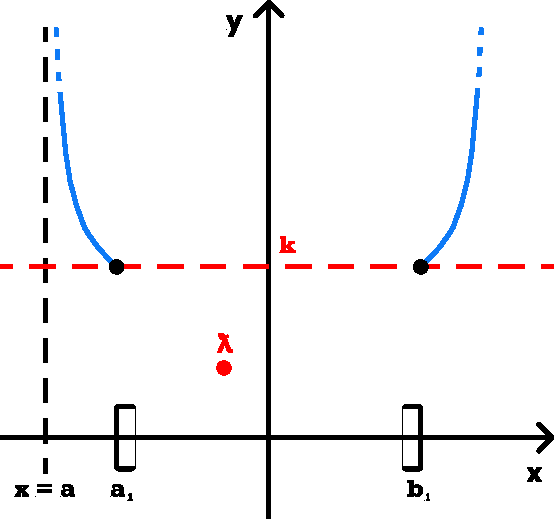
\includegraphics[width=0.9\linewidth]{./images/weierstrassThm.pdf}
\end{wrapfigure}

\noindent Allora $f$ ammette minimo (massimo) globale. \\

\noindent $\implies$ per il teorema di Weierstrass, $f$ è continua in $[a_1, b_1]$ e ammette minimo $\lambda$ in $(a, b)$ (perché al di fuori di $[a_1, b_1]$, $f > k$). In questo esempio però non possiamo dire nulla sul massimo dell'immagine.\\

\noindent\textbf{NB!} Esistono altre varianti del teorema in $[a, b)$ o in $(a, b]$.

\subsection{Teorema degli zeri}
Sia $f: [a, b] \xrightarrow{} \mathbb{R}$, $f$ continua in $[a, b]$ e $f(a)f(b) < 0$. Allora $\exists \Bar{x} \in (a, b) : f(\Bar{x}) = 0$.

\subsubsection{Dimostrazione - metodo dicotomico}
Supponiamo che $f(a) < 0 < f(b)$. Sia ora $c = \frac{a + b}{2}$. Calcoliamo $f(c)$:
\begin{enumerate}
  \item se $f(c) = 0 \implies$ la tesi è vera con $\Bar{x} = c$;
  \item se $f(c) < 0 \implies$ pongo $a_1 = c$, $b_1 = b$ e ho che $f(a_1) < 0 < f(b_1)$;
  \item se $f(c) > 0 \implies$ pongo $a_1 = a$, $b_1 = c$ e ho che $f(a_1) < 0 < f(b_1)$.
\end{enumerate}

\noindent Nei casi \textit{2.} e \textit{3.}, possiamo ripetere il procedimento su $[a_1, b_1]$: calcoliamo nuovamente $c_1 = \frac{a_1 + b_1}{2}$ e valutiamo $f(c_1)$.\\
Per induzione, definiamo $a_n, b_n$ con $a \leq a_n < b_n \leq b$ e $f(a_n) < 0 < f(b_n)$. Osserviamo che $b_1 - a_1 = \frac{b - a}{2}$; $b_2 - a_2 = \frac{b_1 - a_1}{2} = \frac{b - a}{4}$; $b_3 - a_3 = \frac{b_2 - a_2}{2} = \frac{b_1 - a_1}{4} = \frac{b - a}{8}$. In generale, $b_n - a_n = \frac{b - a}{2^n}$ con $n \geq 1$ (ovvero notiamo che viene ristretto sempre di più l'intervallo). Inoltre, per costruzione $a_n \leq a_{n + 1}$ (debolmente crescente) e $b_{n + 1} \leq b_n$ (debolmente decrescente).\\
Per il teorema delle funzioni monotone si ha che:
\begin{align*}
  & \lim_{n \to +\infty} a_n = l \in [a, b] \\
  & \lim_{n \to +\infty} b_n = m \in [a, b]
\end{align*}

\noindent (sia $l$ che $m$ appartengono a $[a, b]$ per il teorema del confronto dato che $a \leq a_n \leq b$ e $a \leq b_n \leq b$). Quindi $\lim_{n \to +\infty} (b_n - a_n) = m - l$. Ma sappiamo anche che $\lim_{n \to +\infty} (b_n - a_n) = \lim_{n \to +\infty} \frac{b - a}{2^n} = 0$. Ciò significa che $m = l$ per il teorema di unicità del limite.\\
Ricordiamo ora che $f(a_n) < 0 < f(b_n)$, ma $\lim_{n \to +\infty} f(a_n) = \lim_{n \to +\infty} f(b_n) = f(l)$ perché $f$ è continua in $[a, b]$.\\
D'altra parte, per il teorema del confronto, da $f(a_n) < 0$ segue che $\lim_{n \to +\infty} f(a_n) \leq 0 \implies f(l) \leq 0$ e, allo stesso modo, da $f(b_n) > 0$ segue che $\lim_{n \to +\infty} f(b_n) \geq 0 \implies f(l) \geq 0$. Pertanto $0 \leq f(l) \leq 0 \implies f(l) = 0$ e quindi, per la tesi, $\Bar{x} = l$.\\

\begin{wrapfigure}{r}{0.3\textwidth}
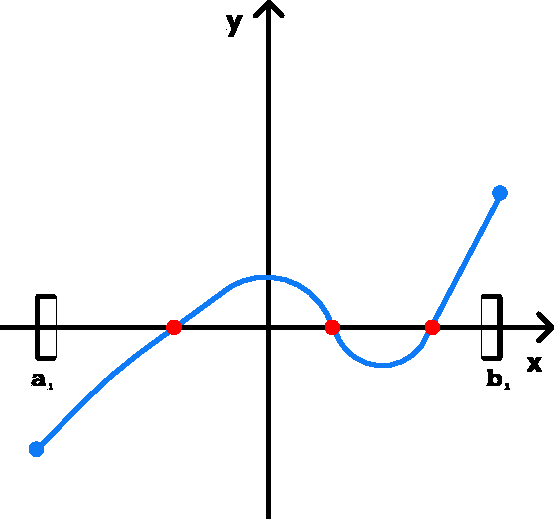
\includegraphics[width=0.9\linewidth]{./images/bolzanoThm.pdf}
\end{wrapfigure}

\noindent\textbf{NB!} Grazie alla monotonia di $a_n, b_n$, abbiamo che $l \in [a_n, b_n] \qquad \forall n \geq 1$. Quindi fissato un $\varepsilon > 0$ e scelto un $n \in \mathbb{N}$ tale per cui $\frac{b - a}{2^n} \ (= b_n - a_n) < \varepsilon$, possiamo approssimare il valore di $l$ a meno di $\varepsilon$.\\

\noindent\textbf{NB!} Può accadere che $f$ abbia più di un punto di azzeramento: 

\subsection{Teorema dei valori intermedi}
Sia $f: I \subset \mathbb{R} \xrightarrow{} \mathbb{R}$, $I$ intervallo, $f$ continua in $I$. Allora $Imm(f)$ è un intervallo.\\

\noindent\textbf{Osservazioni:}
\begin{enumerate}
  \item se $f$ è continua in $I$ con $I = [a, b]$, per il teorema di Weierstrass l'immagine ammette minimo e massimo: $min(Imm(f)) = \lambda \in \mathbb{R}$ e $max(Imm(f)) = \Lambda \in \mathbb{R}$. Contemporaneamente, per il teorema dei valori intermedi, $Imm(f)$ è invervallo. Si ha quindi che $Imm = [\lambda, \Lambda]$;
  \item il teorema degli zeri segue dal teorema di Weierstrass e da quello dei valori intermedi: se $f$ è continua in $I = [a, b]$ e $f(a) < 0 < f(b)$, siccome $f(a), f(b) \in Imm(f)$ e $Imm(f)$ è un intervallo, allora $[f(a), f(b)] \subset Imm(f)$. \\
  Dato che $f(a) < 0 < f(b) \implies 0 \in Imm(f) \implies \exists \Bar{x} \in [a, b] : f(\Bar{x}) = 0$;
  \item il teorema dei valori intermedi vale solo su intervalli. Ad esempio, preso $D_f: [0, 1] \cup [\frac{3}{2}, 3]$ (che non è un intervallo!) e la funzione:
  $$f(x) = \begin{cases}
    x \qquad se \ x \in [0, 1] \\
    2 \qquad se \ x \in [\frac{3}{2}, 3]
  \end{cases}$$ 
  notiamo che $f$ è continua in $D_f$ e $Imm(f) = [0, 1] \cup \{2\}$ che non è un intervallo!
  \item il teorema di Weierstrass vale su un'unione di intervalli disgiunti con gli estremi compresi.
\end{enumerate}

\subsection{Condizione necessaria di estremalità locale interna}
Sia $f: A \subset \mathbb{R} \xrightarrow{} \mathbb{R}$, $x_0 \in A$, $x_0$ interno ad $A$, $x_0$ punto di minimo (massimo) locale, $f$ derivabile in $x_0$. Allora $f'(x_0) = 0$.

\subsubsection{Dimostrazione della condizione necessaria di estremalità locale interna}
Sia $x_0$ punto di minimo locale, ovvero $\exists \delta_1 > 0$ tale che $f(x_0) \leq f(x) \qquad \forall x \in (x_0 - \delta_1, x_0 + \delta_1) \cap A$. Sappiamo poi che $x_0$ è interno ad $A$ quindi $\exists \delta_2 > 0$ tale che $(x_0 - \delta_2, x_0 + \delta_2) \subset A$. Sia quindi $\delta = min(\delta_1, \delta_2)$. \\
Consideriamo ora $x \in (x_0, x_0 + \delta)$ e abbiamo che:
\begin{equation*}
    f'(x_0) = \lim_{x \to x_0} \frac{f(x) - f(x_0)}{x - x_0} = \lim_{x \to x_0^+} \frac{f(x) - f(x_0)}{x - x_0} \geq 0
\end{equation*}

\noindent (dato che $f(x) - f(x_0) \geq 0$ per ipotesi, mentre $x - x_0 > 0$ perché $x \to x_0^+$).\\
Consideriamo ora $x \in (x_0 - \delta, x_0)$ e abbiamo che:
\begin{equation*}
    f'(x_0) = \lim_{x \to x_0} \frac{f(x) - f(x_0)}{x - x_0} = \lim_{x \to x_0^-} \frac{f(x) - f(x_0)}{x - x_0} \leq 0
\end{equation*}

\noindent (dato che $f(x) - f(x_0) \geq 0$ per ipotesi, mentre $x - x_0 < 0$ perché $x \to x_0^-$).\\
Pertanto $0 \leq f'(x_0) \leq 0 \implies f'(x_0) = 0$. \\

\noindent\textbf{NB!} Il "viceversa" è falso, ovvero avere la derivata che si annulla in $x_0$ non implica essere in presenza di un punto di massimo/minimo. Ad esempio, prendiamo $f(x) = x^3$ e calcoliamo la derivata nel punto $x_0 = 0$: $f'(x) = 3x^2 \implies f'(x_0) = 0$. La derivata si annulla, ma $f(x)$ è strettamente crescente per cui non possiede in realtà né massimi, né minimi.\\

\noindent\textbf{NB!} Esistono funzioni che non sono derivabili nei loro minimi: non si può quindi togliere la derivabilità dalle ipotesi del teorema. Ne è un esempio $f(x) = |x|$: $x_0 = 0$ è un punto di minimo globale, ma $\nexists f'(0)$.\\

%\noindent\textbf{NB!} $x_0$ deve essere interno. Ad esempio, presa $f(x) = x$ con $x \in [0, 1]$. Notiamo che $0$ è punto di minimo globale, $1$ è punto di massimo globale e $f'(x) = 1 \qquad \forall x \in [0, 1]$. \\ % da rivedere

\noindent\textbf{Def:} Sia $f: A \subset \mathbb{R} \xrightarrow{} \mathbb{R}$, $x_0 \in A$, $x_0$ interno ad $A$ e $f$ sia derivabile in $x_0$. Diremo che $x_0$ è \textbf{punto stazionario (critico) per $f$} se e solo se $f'(x_0) = 0$.

\subsection{Teorema di Rolle}
Sia $f: [a, b] \xrightarrow{} \mathbb{R}$, $f$ continua in $[a, b]$, $f$ derivabile in $(a, b)$ e $f(a) = f(b)$. Allora $\exists \Bar{x} \in (a, b) : f'(\Bar{x}) = 0$.

\subsubsection{Dimostrazione del teorema di Rolle}
Per il teorema di Weierstrass: $f$ ha punti di minimo globale e punti di massimo globale in $[a, b]$, ovvero $\exists x_1, x_2 \in [a, b] : f(x_1) \leq f(x) \leq f(x_2) \qquad \forall x \in [a, b]$.\\
Se $x_1 = a$ e $x_2 = b$ (o viceversa), dato che $f(a) = f(b)$ (dove $f(a)$ è il minimo globale e $f(b)$ è il massimo globale), allora $f(x) = f(a) \qquad \forall x \in [a, b] \implies f'(x) = 0 \qquad \forall x \in (a, b)$.\\
Se almeno uno tra $x_1$ e $x_2$ non è in un estremo di $[a, b]$: sia, ad esempio, $x_1 \in (a, b)$. Allora $x_1$ è interno ad $[a, b]$. Per la condizione necessaria di estremalità locale, si ha che $f'(x_1) = 0$. Nel caso di $x_2 \in (a, b)$ si replica lo stesso ragionamento.

\subsection{Teorema di Lagrange}
Sia $f: [a, b] \xrightarrow{} \mathbb{R}$, $f$ continua in $[a, b]$, $f$ derivabile in $(a, b)$. Allora $\exists \Bar{x} \in (a, b) : f(b) - f(a) = f'(\Bar{x})(b - a)$.

\subsubsection{Dimostrazione del teorema di Lagrange}
Sia $\varphi(x) = (f(x) - f(a))(b - a) - (f(b) - f(a))(x - a)$: $\varphi$ è continua in $[a, b]$ per composizione di funzioni continue, $\varphi$ è derivabile in $(a, b)$ per composizione di funzioni derivabili. Calcoliamo ora i valori di $\varphi(x)$ agli estremi del dominio:
\begin{equation*}
    \varphi(a) = 0 - 0 = 0 \qquad \qquad \varphi(b) = 0 - 0 = 0
\end{equation*}

\noindent Per il teorema di Rolle: $\exists \Bar{x} \in [a, b] : \varphi'(\Bar{x}) = 0$. Calcoliamo quindi la derivata di $\varphi(x)$:
\begin{equation*}
    \varphi'(x) = f'(x)(b - a) - (f(b) - f(a)) \qquad \forall x \in (a, b)
\end{equation*}

\noindent Sappiamo però che $\varphi'(\Bar{x}) = 0$, quindi $f'(\Bar{x})(b - a) - (f(b) - f(a)) = 0 \iff f'(\Bar{x})(b - a) = f(b) - f(a) \qquad \forall x \in (a, b)$. A livello grafico, significa traslare la retta secante $f(b)$ e $f(a)$ (vedi il link qui sotto). \\

\noindent\textbf{Link:} \href{https://www.geogebra.org/m/z9y24ehK}{Teorema di Lagrange - Interpretazione geometrica}.\\

\noindent\textbf{Corollario 1:} Sia $f: I \subset \mathbb{R} \xrightarrow{} \mathbb{R}$, $I$ intervallo, $f$ derivabile in $I$. Allora $f$ è costante in $I \iff f'(x) = 0 \qquad \forall x \in I$.\\

\noindent Dimostriamo ora il corollario qui sopra. L'implicazione ($\Rightarrow$) è ovvia. Passiamo quindi direttamente alla controimplicazione ($\Leftarrow$). Sia $x_0 \in I$ e sia $x \in I$ con $x \neq x_0$. Supponiamo inoltre che $x > x_0$. Allora prendiamo l'intervallo $[x_0, x] \subset I$ ($I$ intervallo).\\
Dato che $f$ è derivabile in $I$, allora significa che $f$ è continua in $I$ e in tutti i suoi sottoinsiemi, compreso $[x_0, x]$. Inoltre, $f$ è derivabile in $(x_0, x)$. Per il teorema di Lagrange: $\exists \Bar{x} \in [x_0, x] : f(x) - f(x_0) = f'(\Bar{x})(x - x_0) \qquad \forall x \in I \ (x > x_0)$. Ma $\Bar{x} \in (x_0, x) \subset I \implies f'(\Bar{x}) = 0$ per ipotesi. Ciò significa che $f(x) - f(x_0) = 0 \iff f(x) = f(x_0) \qquad \forall x \in I \ (x > x_0)$.\\
Prendiamo ora $x \in I, x < x_0$, abbiamo quindi preso l'intervallo $[x, x_0]$. Per gli stessi motivi enunciati precedentemente, $f$ è continua in $[x, x_0]$ e derivabile in $(x, x_0)$. Possiamo quindi applicare il teorema di Lagrange: $\exists \Bar{x} \in [x, x_0] : f(x_0) - f(x) = f'(\Bar{x})(x_0 - x) \qquad \forall x \in I \ (x < x_0)$. Ma $\Bar{x} \in [x, x_0] \subset I \implies f'(\Bar{x}) = 0$ per ipotesi. Ciò significa che $f(x_0) - f(x) = 0 \iff f(x_0) = f(x) \qquad \forall x \in I \ (x < x_0)$.\\
In conclusione, $f$ è costante in $I$.\\

\noindent\textbf{Teorema:} Sia $f: I \subset \mathbb{R} \xrightarrow{} \mathbb{R}$, $I$ intervallo, $f$ derivabile in $I$. Allora $f$ è debolmente crescente (decrescente) in $I$ se e solo se $f'(x) \underset{(\leq)}{\geq} 0 \qquad \forall x \in I$.\\

\noindent Dimostriamo il teorema qui sopra. Partiamo dall'implicazione ($\Rightarrow$). Sia $f$ debolmente crescente (decrescente) in $I$. Sia $x_0 \in I$, $x \in I$, $x > x_0$, allora $f(x) \underset{(\leq)}{\geq} f(x_0)$.\\
Consideriamo ora $f'(x_0)$:
\begin{equation*}
    f'(x_0) = \lim_{x \to x_0} \frac{f(x) - f(x_0)}{x - x_0} = \lim_{x \to x_0^+} \frac{f(x) - f(x_0)}{x - x_0} \underset{(\leq)}{\geq} 0
\end{equation*}

\noindent (dato che $f(x) - f(x_0) \underset{(\leq)}{\geq} 0$, mentre $x - x_0 > 0$ perché $x \to x_0^+$).

\noindent Allo stesso modo con $x_0 \in I, x_0 > x$ si ha che:
\begin{equation*}
    f'(x_0) = \lim_{x \to x_0} \frac{f(x) - f(x_0)}{x - x_0} = \lim_{x \to x_0^-} \frac{f(x) - f(x_0)}{x - x_0} \underset{(\leq)}{\geq} 0
\end{equation*}

\noindent (dato che $f(x) - f(x_0) \underset{(\geq)}{\leq} 0$, mentre $x - x_0 < 0$ perché $x \to x_0^-$).\\
Dimostriamo ora la controimplicazione ($\Leftarrow$). Per ipotesi $f'(x) \underset{(\leq)}{\geq} 0 \qquad \forall x \in I$.\\
Siano ora $x_1, x_2 \in I$ con $x_1 < x_2$. Dato che $f$ è derivabile in $I$, allora $f$ è continua in $I$ e in tutti i suoi sottoinsiemi, compreso $[x_1, x_2]$. Mentre $f$ è derivabile in $(x_1, x_2)$.\\
Per il teorema di Lagrange, $\exists \Bar{x} \in (x_1, x_2) \subset I$ tale che $f(x_2) - f(x_1) = f'(\Bar{x})(x_2 - x_1) \underset{(\leq)}{\geq} 0$ (dato che $(x_2 - x_1) > 0$ e $f'(\Bar{x}) \underset{(\leq)}{\geq} 0$). Ossia $f(x_2) - f(x_1) \underset{(\leq)}{\geq} 0 \iff f(x_2) \underset{(\leq)}{\geq} f(x_1) \implies f$ è debolmente crescente (decrescente) in $I$.\\

\noindent\textbf{Teorema:} Sia $f: I \subset \mathbb{R} \xrightarrow{} \mathbb{R}$, $I$ intervallo, $f$ derivabile in $I$. Se $f'(x) \underset{(<)}{>} 0 \qquad \forall x \in I$ allora $f$ è strettamente crescente (decrescente).\\

\noindent Dimostriamo il teorema qui sopra. Per ipotesi abbiamo che $f'(x) \underset{(<)}{>} 0 \qquad \forall x \in I$. Prendiamo ora $x_1, x_2 \in I$ con $x_1 < x_2 \implies [x_1, x_2] \subset I \implies f$ continua su $[x_1, x_2]$ e $f$ derivabile su $(x_1, x_2)$.\\
Per il teorema di Lagrange, si ha che $\exists \Bar{x} \in [x_1, x_2] : f(x_2) - f(x_1) = f'(\Bar{x})(x_2 - x_1) \underset{(<)}{>} 0$ (dato che $(x_2 - x_1) > 0$ e $f'(\Bar{x}) \underset{(<)}{>} 0$). Quindi si ha che $f(x_2) \underset{(<)}{>} f(x_1)$.

\subsection{Condizioni sufficienti di estremalità locale}
Sia $f: I \subset \mathbb{R} \xrightarrow{} \mathbb{R}$, $I$ intervallo, $x_0 \in I$, $x_0$ interno ad $I$, $f$ continua in $I$, $f$ derivabile in $I - \{x_0\}$. Allora:
\begin{enumerate}
    \item se $\exists \delta > 0$ tale che $f'(x) \geq 0$ per $x \in (x_0 - \delta, x_0)$ e $f'(x) \leq 0$ per $x \in (x_0, x_0 + \delta)$, segue che $x_0$ è punto di massimo locale;
    \item se $\exists \delta > 0$ tale che $f'(x) \leq 0$ per $x \in (x_0 - \delta, x_0)$ e $f'(x) \geq 0$ per $x \in (x_0, x_0 + \delta)$, segue che $x_0$ è punto di minimo locale;
\end{enumerate}

\noindent Dimostriamo ora il punto \textit{1.} qui sopra. Sia $x \in (x_0 - \delta, x_0) \subset I$. Consideriamo quindi $[x, x_0] \implies f$ è continua in $[x, x_0]$ e derivabile in $(x, x_0)$.\\
Per il teorema di Lagrange, $\exists \Bar{x} \in [x, x_0] : f(x_0) - f(x) = f'(\Bar{x})(x_0 - x) \geq 0$ (dato che $f'(\Bar{x}) \geq 0$ per ipotesi e $(x_0 - x) > 0$). Quindi $f(x_0) \geq f(x) \qquad \forall x \in (x_0 - \delta, x_0)$.\\
Sia ora $x \in (x_0, x_0 + \delta)$. Consideriamo quindi $[x_0, x] \implies f$ è continua in $[x_0, x]$ e derivabile in $(x_0, x)$. \\
Per il teorema di Lagrange, $\exists \Bar{x} \in [x_0, x] : f(x) - f(x_0) = f'(\Bar{x})(x - x_0) \leq 0$ (dato che $f'(\Bar{x}) \leq 0$ per ipotesi e $(x - x_0) > 0$). Quindi $f(x_0) \leq f(x) \qquad \forall x \in (x_0, x_0 + \delta)$.\\
In conclusione, $f(x) \leq f(x_0) \qquad \forall x \in (x_0 - \delta, x_0 + \delta)$.\\

\noindent\textbf{Def:} Sia $f: A \subset \mathbb{R} \xrightarrow{} \mathbb{R}$, $x_0 \in A$ è detto \textbf{punto di minimo (massimo) locale forte per $f$} se e solo se $\exists U_{x_0}$ intorno di $x_0$ tale che $f(x) \underset{(<)}{>} f(x_0) \qquad \forall x \in (U_{x_0} \cap A) - \{x_0\}$.

\subsection{Condizioni di estremalità del secondo ordine}
\textbf{Teorema: } Sia $I \subset \mathbb{R}$, $I$ intervallo, $f: I \xrightarrow{} \mathbb{R}$, $x_0 \in I$, $f$ derivabile in $I$ e $\exists f''(x_0)$. Allora:
\begin{enumerate}[label=\alph*)]
    \item se $f'(x_0) = 0$ e $f''(x_0) \underset{(<)}{>} 0$ si ha che $x_0$ è punto di minimo (massimo) locale forte (condizione sufficiente di estremalità);
    \item se $x_0$ è punto di minimo (massimo) locale, con $x_0$ interno ad $I$, allora $f'(x_0) = 0$ e $f''(x_0) \underset{(\leq)}{\geq} 0$ (condizione necessaria di estremalità).
\end{enumerate}

\subsubsection{Dimostrazione della condizione sufficiente di estremalità del secondo ordine}
Sia $f''(x_0) \underset{(<)}{>} 0$. Utilizziamo la formula di Taylor di ordine $2$, centrata in $x_0$, con resto di Peano:
\begin{equation*}
    f(x) = f(x_0) + f'(x_0)(x - x_0) + \frac{f''(x_0)}{2} \cdot (x - x_0)^2 + o((x - x_0)^2) \ per \ x \to x_0
\end{equation*}

\noindent $f'(x_0) = 0$ per ipotesi e, se $x \neq x_0$, abbiamo che:
\begin{equation*}
    \frac{f(x) - f(x_0)}{(x - x_0)^2} =  \frac{f''(x_0)}{2} + o(1) \ per \ x \to x_0
\end{equation*}

\noindent Quindi:
\begin{equation*}
    \lim_{x \to x_0} \frac{f(x) - f(x_0)}{(x - x_0)^2} = \frac{f''(x_0)}{2} \underset{(<)}{>} 0
\end{equation*}

\noindent Per il teorema di permanenza del segno, $\exists U_{x_0}$ intorno di $x_0$ tale che $\frac{f(x) - f(x_0)}{(x - x_0)^2} \underset{(<)}{>} 0 \qquad \forall x \in (U_{x_0} \cap A) - \{x_0\}$. \\
Dato che $(x - x_0)^2 > 0$ per $x \neq x_0$, allora $f(x) \underset{(<)}{>} f(x_0) \qquad \forall x \in (U_{x_0} \cap A) - \{x_0\}$, ovvero $x_0$ è punto di minimo (massimo) locale forte.

\subsubsection{Dimostrazione della condizione necessaria di estremalità del secondo ordine}
Per la condizione necessaria di estremalità locale del primo ordine si ha che $f'(x_0) = 0$. Sia ora $x_0$ punto di minimo locale. Se avessimo $f''(x_0) < 0$, allora potremmo applicare la condizione sufficiente di estremalità del secondo ordine (punto \textit{a)}). Per cui $x_0$ sarebbe punto di massimo locale forte, ovvero $\exists V_{x_0}$ intorno di $x_0 : f(x_0) \leq f(x) \qquad \forall x \in (V_{x_0} \cap A)$.\\
Se prendiamo però $x \in (V_{x_0} \cap U_{x_0}) \cap A$, allora $f(x) < f(x_0) \leq f(x)$ il che è chiaramente falso. \\
Dato che siamo giunti ad una contraddizione, significa che la supposizione di partenza $f''(x_0) < 0$ è falsa, ovvero in realtà si ha che $f''(x_0) > 0$.

\subsection{Teorema delle derivate successive}
Sia $n \in \mathbb{N}, n \geq 1, f \in C^{n - 1}(I), I$ intervallo, $x_0 \in I, x_0$ interno ad $I$ (sono le ipotesi necessarie per applicare Taylor). Supponiamo ora che $\exists f^{(n)}(x_0)$ e che $f^{(k)}(x_0) = 0$ per $k = 1, 2, ..., n - 1$ e che $f^{(n)}(x_0) \underset{(<)}{>} 0$. Allora:
\begin{enumerate}
    \item se $n$ è pari, si ha che $x_0$ è punto di minimo (massimo) locale forte a seconda che $f^{(n)}(x_0)$ sia positiva o negativa;
    \item se $n$ è dispari, $x_0$ non è né punto di massimo locale, né punto di minimo locale.
\end{enumerate}

\subsection{Periodicità}
\textbf{Def:} Sia $f: A \subset \mathbb{R} \xrightarrow{} \mathbb{R}$ e sia $T > 0$. Diremo che $T$ è un periodo per $f$ se e solo se $\forall x \in A$ si ha che $x + T \in A$ ed inoltre $f(x) = f(x + T)$.\\
Sia $p = min\{T > 0 : T \ periodo \ per \ T\}$, se esiste. $p$ è detto \textbf{minimo periodo di $f$}. Se $f$ ha minimo periodo $p$ è detta \textbf{periodica di periodo $p$} (oppure ha periodo $p$).\\

\noindent\textbf{Osservazioni:} 
\begin{enumerate}
    \item Le funzioni costanti ammettono $T$ reale positivo, ma non possiedono un minimo periodo (perché il minimo sarebbe $0$, ma i periodi sono esclusivamente positivi);
    \item Se $f$ è periodica, allora $D_f$ è illimitato e $f$ non è iniettiva (al contrario, se $D_f$ è limitato, allora $f$ non è periodica);
    \item Se $f$ ha periodo $p$, allora è sufficiente studiarla in $[x_0, x_0 + p] \cap D_f$, dove $x_0 \in D_f$.\\
    Inoltre, $\mathcal{G}(f)$ si ottiene traslando da $\mathcal{G}(f/[x_0, x_0 + p])$ mediante traslazione (la scrittura $f/[x_0, x_0 + p]$ significa prendere $f$ e restringere il suo dominio a $[x_0, x_0 + p]$);
    \item se $f$ ha periodo $p$, allora $f(ux)$ con $u \neq 0$ ha periodo $\frac{p}{|u|}$;
    \item se $f, g$ hanno periodo $p$, allora $f + g$, $f \cdot g$, $\frac{f}{g}$ con $g \neq 0$ hanno periodo minore o uguale a $p$ (ad esempio, $\sin(x)$ ha periodo $2\pi$, $\cos(x)$ ha periodo $2\pi$, ma $\tan(x) = \frac{\sin(x)}{\cos(x)}$ ha periodo $\pi$);
    \item se $f$ ha periodo $p$ e $g$ si può comporre con $f$, allora $g \circ f$ ha periodo minore o uguale a $p$.
\end{enumerate}

\subsection{Asintoti}
\textbf{Asintoto verticale - Def:} Sia $f: A \subset \mathbb{R} \xrightarrow{} \mathbb{R}$, $x_0 \in \mathbb{R}$ di accumulazione da destra (sinistra) per $A$. La retta di equazione $x = x_0$ è \textbf{asintoto verticale destro (sinistro) per $f$} se e solo se:
\begin{equation*}
    \lim_{\underset{\scriptstyle (x \to x_0^-)}{x \to x_0^+}} f(x) = \begin{cases}
        +\infty \\
        -\infty
    \end{cases}
\end{equation*}

\noindent Se $x = x_0$ è sia asintoto verticale destro che sinistro si dice asintoto verticale.\\

\noindent\textbf{Asintoto orizzontale - Def:} Sia $f: A \subset \mathbb{R} \xrightarrow{} \mathbb{R}$ e sia $+\infty \ (-\infty)$ punto di accumulazione per $A$. La retta di equazione $y = l$ è \textbf{asintoto orizzontale a $+\infty \ (-\infty)$ per $f$} se e solo se:
\begin{equation*}
    \lim_{\underset{\scriptstyle (x \to -\infty)}{x \to +\infty}} f(x) = l \in \mathbb{R}
\end{equation*}

\noindent\textbf{NB!} Una funzione continua su $\mathbb{R}$ che ammette asintoto orizzontale a $+\infty$ e a $-\infty$ è limitata.\\

\noindent\textbf{Asintoto obliquo - Def:} Sia $f: A \subset \mathbb{R} \xrightarrow{} \mathbb{R}$ e sia $+\infty \ (-\infty)$ un punto di accumulazione per $A$. Diremo che la retta di equazione $y = mx + n$, con $m, n \in \mathbb{R}$ e $m \neq 0$, è \textbf{asintoto obliquo a $+\infty \ (-\infty)$ per $f$} se e solo se:
\begin{equation*}
    \lim_{\underset{\scriptstyle (x \to -\infty)}{x \to +\infty}} (f(x) - (mx + n)) = 0
\end{equation*}

\noindent (la scrittura precedente può anche essere scritta come $f(x) = mx + n + o(1) \ per \ x \to +\infty \ (-\infty)$). Dalla definizione precedente segue che:
\begin{equation*}
    0 = \lim_{\underset{\scriptstyle (x \to -\infty)}{x \to +\infty}} \frac{f(x) - (mx + n)}{x} = \lim_{\underset{\scriptstyle (x \to -\infty)}{x \to +\infty}} \left(\frac{f(x)}{x} - m - \frac{n}{x}\right) \implies \lim_{\underset{\scriptstyle (x \to -\infty)}{x \to +\infty}} \frac{f(x)}{x} = m \in \mathbb{R} - \{0\}
\end{equation*}

\noindent Inoltre:
\begin{equation*}
    \lim_{\underset{\scriptstyle (x \to -\infty)}{x \to +\infty}} (f(x) - mx) = \lim_{\underset{\scriptstyle (x \to -\infty)}{x \to +\infty}} (f(x) - (mx + n) + n) = n \in \mathbb{R}
\end{equation*}

\noindent (dato che $f(x) - (mx + n) \to 0$ per la definizione di asintoto obliquo).

\subsection{Convessità}
\textbf{Def:} Sia $I \subset \mathbb{R}$ un intervallo e siano $x_1, x_2 \in I$ con $x_1 < x_2$. Diremo \textbf{combinazione convessa di $x_1, x_2$} la quantità $x(t) = (1 - t)x_1 + tx_2$ al variare di $t \in [0, 1]$ (la precedente quantità è costruita in modo che la somma tra i coefficienti di $x_1$ ($(1 - t)$) e $x_2$ ($t$) dia come risultato $1$).\\

\noindent\textbf{Def:} Sia $f: I \subset \mathbb{R} \xrightarrow{} \mathbb{R}$, $I$ intervallo. $f$ è \textbf{convessa in $I$} se e solo se $\forall x_1, x_2 \in I$ con $x_1 < x_2$ e $\forall t \in [0, 1]$ si ha che: $f(x(t)) \leq (1 - t)f(x_1) + tf(x_2)$.\\
Diremo che $f$ è \textbf{concava in $I$} se e solo se $(-f)$ è convessa.\\

\begin{wrapfigure}{l}{0.4\textwidth}
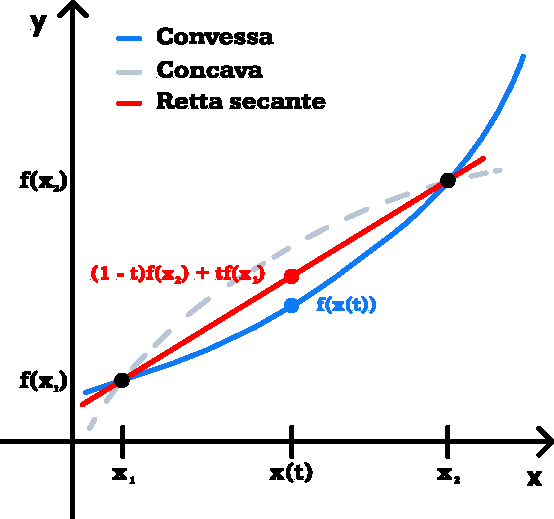
\includegraphics[width=0.9\linewidth]{./images/convexity.pdf}
\end{wrapfigure}

\noindent\textbf{Teorema:} Se $f$ è convessa in $I$ allora $f$ è continua nei punti interni a $I$. \\

\noindent\textbf{Teorema:} Sia $f: I \subset \mathbb{R} \xrightarrow{} \mathbb{R}$, derivabile in $I$, $I$ intervallo. Allora le seguenti sono condizioni equivalenti:
\begin{enumerate}[label=\alph*)]
    \item $f$ è convessa (concava in $I$); 
    \item $\forall x_0, x \in I$ si ha che $f(x) \underset{(\leq)}{\geq} f(x_0) + f'(x_0)(x - x_0)$ (ovvero $f$ "sta sopra" alle rette tangenti);
    \item $f'(x)$ è debolmente crescente (decrescente) in $I$.
\end{enumerate}

\noindent\textbf{Teorema:} Sia $f: I \subset \mathbb{R} \xrightarrow{} \mathbb{R}$ derivabile due volte in $I$, $I$ intervallo. Allora $f$ è convessa (concava) in $I \iff f'(x) \underset{(\leq)}{\geq} 0 \qquad \forall x \in I$. \\

\noindent\textbf{Punti di flesso - Def:} Sia $f: I \subset \mathbb{R} \xrightarrow{} \mathbb{R}, I$ intervallo. $x_0 \in I$ è \textbf{punto di flesso per $f$} se e solo se $\exists \delta > 0$ tale che $f$ sia convessa in $(x_0 - \delta, x_0)$ e $f$ sia concava in $(x_0, x_0 + \delta)$ o viceversa.\\

\noindent\textbf{Teorema:} Sia $f: I \subset \mathbb{R} \xrightarrow{} \mathbb{R}$, $I$ intervallo. Sia $f$ derivabile due volte in $I$ e sia $x_0$ un punto di flesso interno ad $I$. Allora $f''(x_0) = 0$.
\end{document}